% ----------------------------------
% Cap Análisis
% ----------------------------------
%	Incluye
%		Casos de uso
%
\documentclass[a4paper,oneside,11pt]{book}

\usepackage[spanish,activeacute]{babel}
\usepackage[utf8]{inputenc}
%\usepackage[T1]{fontenc}
\usepackage{tabulary}
\usepackage{graphicx}
\usepackage{color}
\usepackage{colortbl}
\usepackage{float}

\oddsidemargin=0.2cm
\headsep=1cm
\textheight=21cm
\textwidth=16cm

\setcounter{secnumdepth}{3}

\definecolor{gris}{gray}{0.80}
\definecolor{gris2}{gray}{0.90}
\definecolor{negro}{gray}{0}

% Personalizamos la separación entre párrafos...
\parskip=6pt

% Personalizamos el identado en la primera línea del nuevo párrafo...
\parindent=10pt

\begin{document}
	
\chapter{Casos de uso} % (fold)
	\label{cha:casos_de_uso}

% 
% Sec Tipos de usuarios
%
\section{Modelo de casos de uso} % (fold)
	\label{sec:modelo_casos_de_uso}
	
		En esencia, un caso de uso narra una historia estilizada sobre cómo interactúa un usuario final (que tiene cierto número de roles posibles) con el sistema en circunstancias específicas. La historia puede ser un texto narrativo, un lineamiento de tareas o interacciones, una descripción basada en un formato o una representación diagramática. Sin importar su forma, \textbf{un caso de uso ilustra el software o sistema desde el punto de vista del usuario final.}
		
		\medskip
		\fcolorbox{negro}{gris}{\parbox{15cm}{Los \textit{Casos de Uso} no son parte del diseño (cómo), sino parte del análisis (qué). De esta forma nos ayudan a describir qué es lo que es sistema debe hacer desde el punto de vista del usuario. Es decir, describen un uso del sistema y cómo éste interactúa con el usuario.}}
		
		\medskip		
		El primer paso para escribir un caso de uso es \textbf{definir un conjunto de <<actores>>.} que estarán involucrados en la historia. Los \textit{actores} son las distintas personas (o dispositivos) que usan el sistema o producto en el contexto de la función y comportamiento que va a describirse. Los actores representan los papeles que desempeñan las personas (o dispositivos) cuando opera el sistema. Con una definición más formal, un \textit{actor} es cualquier cosa que se comunique con el sistema o producto y que sea externo a éste. Todo actor tiene uno o más objetivos cuando utiliza el sistema.
		
		 En este documento nos centraremos en los diagramas UML y en la descripción formal de los casos de uso. La representación con diagramas facilita la comprensión. Cada caso de uso está representado por un óvalo. Por su parte, la descripción se hará de manera formal. Como cualquier otra forma de descripción escrita, un caso de uso tiene sus limitaciones, y si la descripción es poco clara, el caso de uso será confuso o ambiguo. Por ello, se intentará mostrar un nivel de detalle y precisión significativos para que la comprensión sea la mejor posible.
		
	
	\section{Diagramas de casos de uso} % (fold)
	\label{sub:diagramas_de_casos_de_uso}
	
		Los diagramas de casos de uso que forman la aplicación están agrupados principalmente en seis paquetes.
		\begin{itemize}
			\item \textit{Actores}. Principales personas que se comunican con el sistema.
			\item \textit{Actividades Generales}. Muestra todas las actividades que pueden los usuarios y para las cuales no es necesario estar registrado.
			\item \textit{Actividades de los médicos}. Todo lo referente a la funcionalidad que el médico espera del sistema.
			\item \textit{Actividades de los pacientes}. Todas aquellas actividades que pueden realizar los usuarios registrados con el rol de paciente.
			\item \textit{Gestión de fichas médicas}. Abarca todas las operaciones que pueden realizar los usuarios registrados, tanto médicos como pacientes, sobre las fichas médicas.
			\item \textit{Panel del Administrador}. Funcionalidades asociadas al Administrador del sistema.
		\end{itemize}
	
		\fbox{\parbox{15cm}{No todos los casos de uso serán implementados durante la primera iteración. En la documentación y descripción de los casos de uso que se trata en el siguiente apartado se verá de manera más detallada.}}
	
		\subsection{Actores} % (fold)
		\label{sec:actores}
			Podemos observar que existen tres tipos de actores principales (Figura \ref{fig:actores}), un usuario genérico, un administrador y un usuario registrado. De éste último heredan otros dos tipos de actores, los médicos y los pacientes.
			\begin{figure}[H]
			  \centering
			    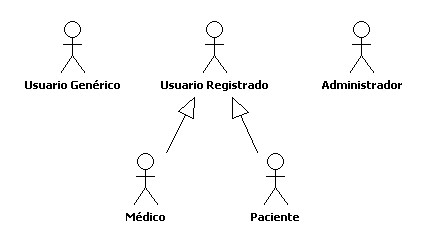
\includegraphics[width=10cm]{img/jpg/casos_uso/Actores.jpg}
			  \caption{Actores.}
			  \label{fig:actores}
			\end{figure}
			
			
		% section actores (end)
	
		\subsection{Actividades Generales} % (fold)
		\label{sec:actividades_generales}
		
			Las actividades generales son una serie de acciones que puede hacer un actor genérico del sistema, es decir, aquellos que no necesitan estar identificados en el sistema.
			\paragraph{Registro e información} % (fold)
			\label{par:registro_e_informacion}
				Un usuario genérico podrá registrarse como médico o como paciente. Una vez registrado deberá rellenar su información personal, y opcionalmente, adjuntar una foto para su perfil. (Figura \ref{fig:reg_inf}). Además, si es médico, deberá rellenar la información de su consulta.
				\begin{figure}[H]
				  \centering
				    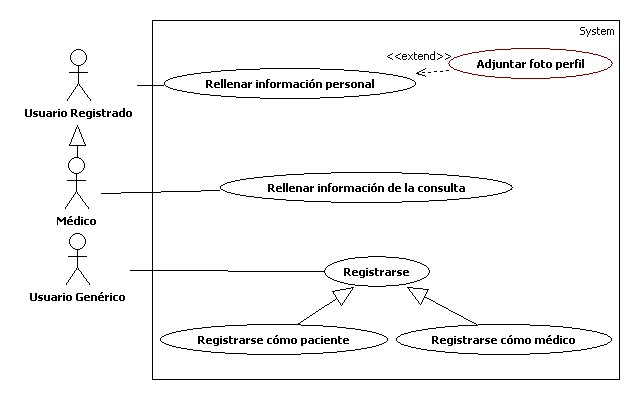
\includegraphics[width=14cm]{img/jpg/casos_uso/Registro_e_informacion.jpg}
				  \caption{Registro e información.}
				  \label{fig:reg_inf}
				\end{figure}
			% paragraph registro_e_información (end)
			
			\paragraph{Características generales} % (fold)
			\label{par:caracteristicas_generales}
				Las características generales (Figura \ref{fig:caracteristicas}) son una serie de acciones que puede realizar un actor genérico para ver diversa información de la aplicación o para interactuar con ella, en algunos casos.
							
			% paragraph características_generales (end)
		
			\paragraph{Acceso y Autentificación} % (fold)
			\label{par:acceso_y_autentificacion}
				Son funcionalidades que pueden realizar los actores registrados para iniciar o cerrar sesión (Figura \ref{fig:acceso}). Además, existe la posibilidad de no cerrar sesión. Otra función es la de recordar contraseña
				\begin{figure}[H]
				  \centering
				    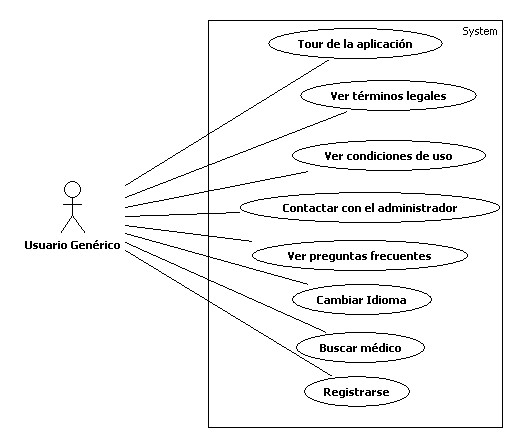
\includegraphics[width=12cm]{img/jpg/casos_uso/Generales.jpg}
				  \caption{Características Generales.}
				  \label{fig:caracteristicas}
				\end{figure}
				
				\begin{figure}[H]
				  \centering
				    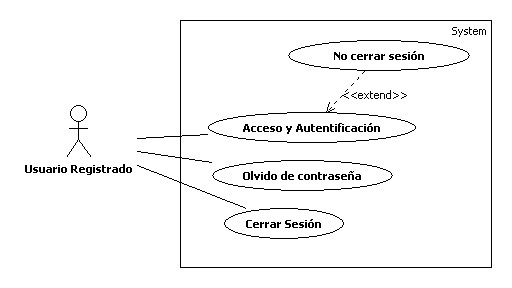
\includegraphics[width=12cm]{img/jpg/casos_uso/Acceso_y_Autentificacion.jpg}
				  \caption{Acceso y Autentificación.}
				  \label{fig:acceso}
				\end{figure}
			% paragraph acceso_y_autentificación (end)
			
		% section actividades_generales (end)
	
	
		\subsection{Actividades de los médicos} % (fold)
		\label{sec:actividades_de_los_medicos}
		
			Pretenden abordar todas las acciones que puede realizar un actor registrado identificado en el sistema con el rol de médico.
			\paragraph{Panel de Configuración de los médicos} % (fold)
			\label{par:panel_de_configuracion_de_los_medicos}
				Un médico tiene acceso a un panel de configuración (Figura \ref{fig:config_med}) desde el cual modificar los datos personales y de su consulta médica (Figura \ref{fig:config_med_datos}), modificar los datos de su cuenta (Figura \ref{fig:config_med_cuenta}), configurar su horario de disponibilidad, las notificaciones que recibirá en función de diversos sucesos y los motivos que incluirá en su facturas.
				
				Respecto a los datos, cabe destacar que podrá adjuntar, modificar o crear su propio curriculum, y una foto de su perfil. Respecto a la cuenta, que podrá cambiar su contraseña, su email, el idioma y darse de baja en el servicio cuando lo desee.
				
				Siempre que se modifiquen sus datos o la información de su cuenta, se almacerá la acción realizada en un historial del médico, que contendrá toda la información relevante de la que pueda ser interesante mantener un registro.
				\begin{figure}[H]
				  \centering
				    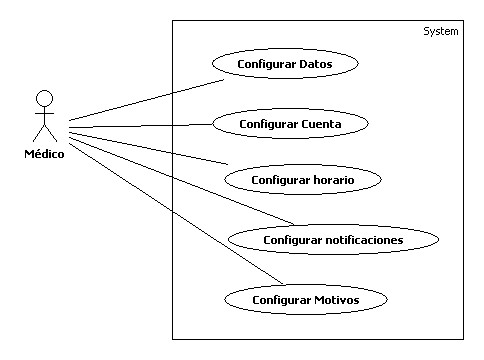
\includegraphics[width=12cm]{img/jpg/casos_uso/Configuracion_Medico.jpg}
				  \caption{Panel de configuración de los médicos.}
				  \label{fig:config_med}
				\end{figure}
				
				\begin{figure}[H]
				  \centering
				    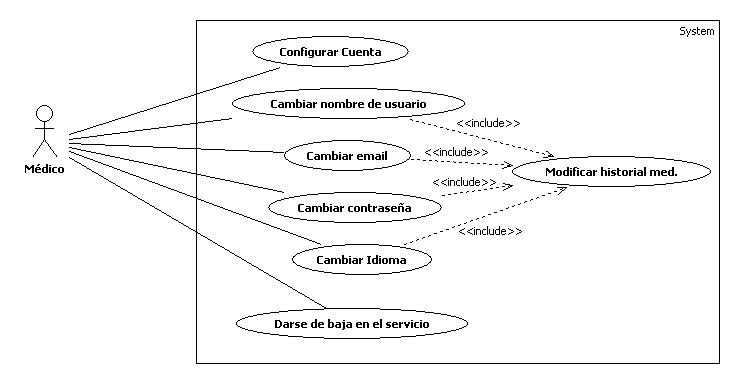
\includegraphics[width=15cm]{img/jpg/casos_uso/Configurar_Cuenta_Medico.jpg}
				  \caption{Configurar cuenta del médico.}
				  \label{fig:config_med_cuenta}
				\end{figure}
				
				\bigskip
				
				\begin{figure}[H]
				  \centering
				    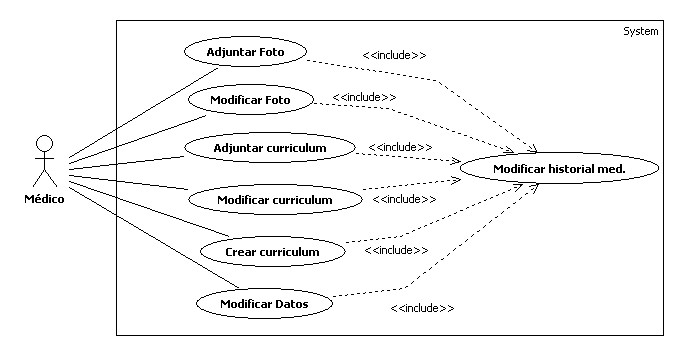
\includegraphics[width=15cm]{img/jpg/casos_uso/Configurar_Datos_Medico.jpg}
				  \caption{Configurar los datos del médico.}
				  \label{fig:config_med_datos}
				\end{figure}
			% paragraph panel_de_configuración_de_los_médicos (end)
		
			\bigskip
			\bigskip
			\paragraph{Gestión del Calendario del médico} % (fold)
			\label{par:gestion_del_calendario_del_medico}
			
				Un actor médico puede realizar una serie de acciones relacionadas con su calendario (Figura \ref{fig:cal_med}), entre ellas realizar la vista diaria, semanal o mensual de las citas que tiene concertadas. Desde todas las vistas podrá acceder a la vista de la ficha médica del paciente o anular una cita puntual (modificará el historial del médico y el del paciente). Por otro lado, debe configurar su horario de disponibilidad para que esté visible por los posibles pacientes potenciales y configurar las notificaciones que le llegarán al email. Por último, puede anular un día entero. La modificación de cualquiera de las tres últimas funcionalidades es relevante, y quedará registrada en el historial del médico.
				\begin{figure}[H]
				  \centering
				    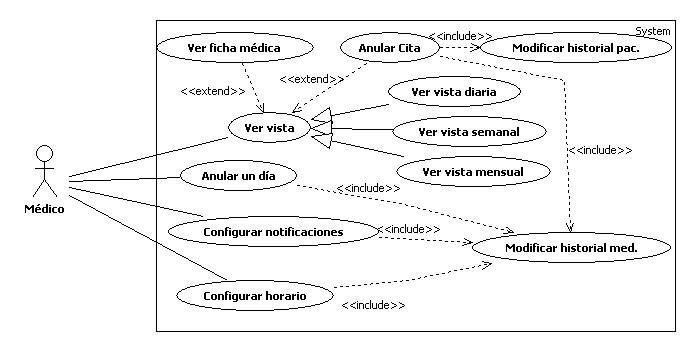
\includegraphics[width=14cm]{img/jpg/casos_uso/Gestion_calendario.jpg}
				  \caption{Gestión del Calendario del médico.}
				  \label{fig:cal_med}
				\end{figure}
			% paragraph gestión_del_calendario_del_médico (end)
		
			\paragraph{Gestión de pacientes} % (fold)
			\label{par:gestion_de_pacientes}
				Un actor médico puede ver una lista de todos sus pacientes o buscar pacientes en función de diversos filtros. Cuando haya encontrado al paciente deseado, podrá acceder a su ficha médica.
				\begin{figure}[H]
				  \centering
				    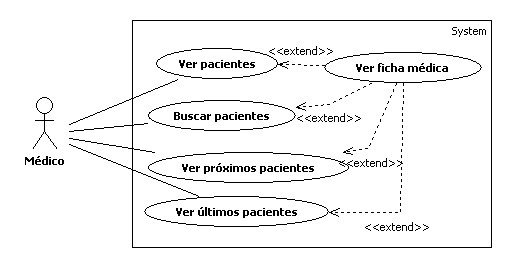
\includegraphics[width=10cm]{img/jpg/casos_uso/Gestion_Pacientes.jpg}
				  \caption{Gestión Pacientes del médico.}
				  \label{fig:pac_med}
				\end{figure}
			% paragraph gestión_de_pacientes (end)
		
			\paragraph{Gestión de estadísticas} % (fold)
			\label{par:gestion_de_estadisticas}
				Un actor médico puede ver una serie de estadísticas generales del último mes, del último año o de los últimos años. Además, puede ver estadísticas más concretas sobre pacientes, diagnósticos o beneficios(Figura \ref{fig:estad_med}). 
				
			% paragraph gestión_de_estadísticas (end)
			
			\paragraph{Gestión de Plantillas} % (fold)
			\label{par:gestion_de_plantillas}
				Siempre es muy útil que un actor médico pueda generar una serie de plantillas de diversos tipos (Figura \ref{fig:plan_med}). Con ellas ahorrará tiempo a la hora de escribir diagnósticos, tratamientos u otros documentos. La información referente a la creación, modificación o eliminación de plantillas es algo que quedará reflejado en el historial del médico.
				
			% paragraph gestión_de_plantillas (end)
			
			\paragraph{Administración y Gestión del Centro médico} % (fold)
			\label{par:administracion_y_gestion_del_centro_medico}
				
				(Figura \ref{fig:ad_ges_med}) Un médico puede anotar todos sus ingresos y sus gastos para ver un balance de la economía. También podrá buscar la factura que sea necesaria. Otra cosa que podrá administrar serán los votos recibidos por los distintos pacientes a los que ya haya visitado. Por último, podrá acceder al historial y realizar búsquedas mediante distintos filtros de toda la información relevante resultado de alguna acción de la aplicación. Lo relacionado a añadir ingresos o gastos actualizará el historial del médico. Además, siempre que se anote un ingreso, se generará una factura asociada.
				
				\begin{figure}[H]
				  \centering
				    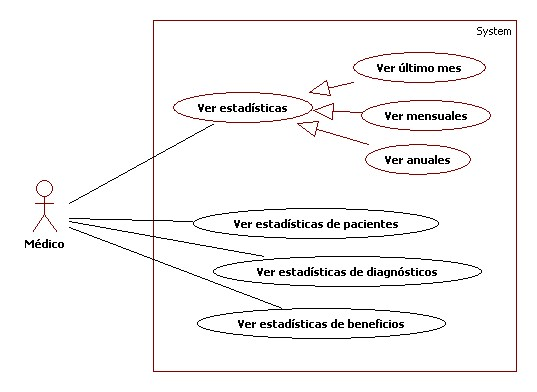
\includegraphics[width=12cm]{img/jpg/casos_uso/Estadisticas.jpg}
				  \caption{Gestión de Estadísticas de los médicos.}
				  \label{fig:estad_med}
				\end{figure}
				
				\begin{figure}[H]
				  \centering
				    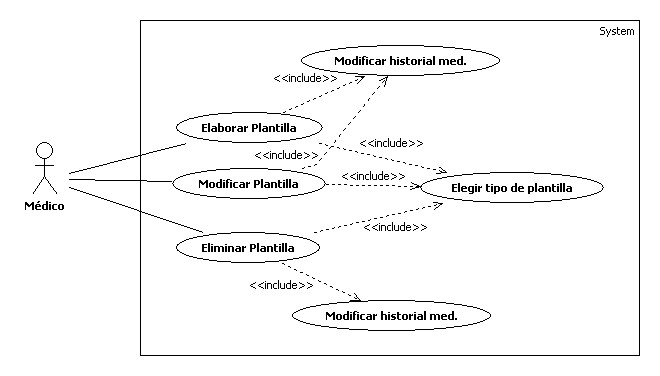
\includegraphics[width=14cm]{img/jpg/casos_uso/Gestion_plantillas.jpg}
				  \caption{Gestión de Plantillas de los médicos.}
				  \label{fig:plan_med}
				\end{figure}
				
				\begin{figure}[H]
				  \centering
				    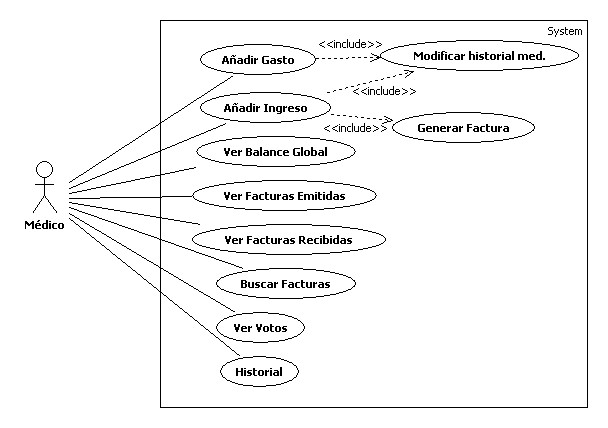
\includegraphics[width=14cm]{img/jpg/casos_uso/Administracion_y_Gestion.jpg}
				  \caption{Administración y Gestión del centro médico.}
				  \label{fig:ad_ges_med}
				\end{figure}
			% paragraph administración_y_gestión_del_centro_médico (end)
					
		% section actividades_de_los_médicos (end)
	
		\subsection{Actividades de los pacientes} % (fold)
		\label{sec:actividades_de_los_pacientes}
		Pretenden abordar todas las acciones que puede realizar un actor registrado identificado en el sistema con el rol de paciente.
			\paragraph{Calendario del Paciente} % (fold)
			\label{par:calendario_del_paciente}
				Un actor paciente puede realizar una serie de acciones relacionadas con su calendario (Figura \ref{fig:cal_pac}), entre ellas realizar la vista diaria, semanal o mensual de las citas que tiene concertadas. Desde todas las vistas podrá acceder a la información del médico o anular una cita puntual. Por otro lado, debe configurar las notificaciones que le llegarán al email. Siempre que anule una cita o que modifique la configuración de sus notificaciones, se registrarán los cambios en el historial del paciente.
				\begin{figure}[H]
				  \centering
				    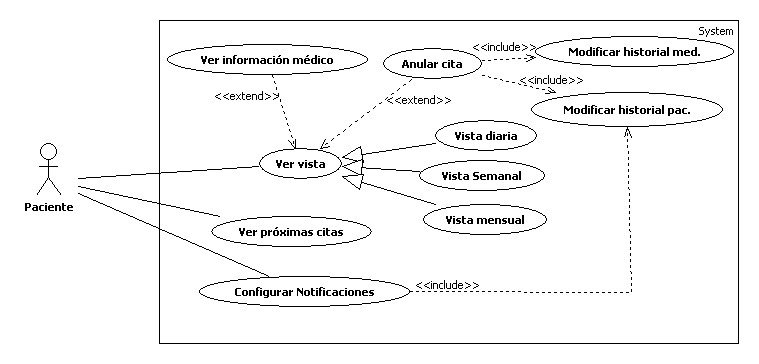
\includegraphics[width=14cm]{img/jpg/casos_uso/Calendario_del_paciente.jpg}
				  \caption{Calendario del Paciente.}
				  \label{fig:cal_pac}
				\end{figure}
			% paragraph calendario_del_paciente (end)
		
			\paragraph{Gestión de médicos del paciente} % (fold)
			\label{par:gestion_de_medicos_del_paciente}
			
				(Figura \ref{fig:med_pac}) Un actor paciente puede ver una lista con todos sus médicos o buscarlos según diversos filtros. Posee una serie de especialistas asignados a una lista de favoritos, para poder acceder a ellos más rápidamente. Una vez encontrado el médico deseado, podrá ver su horario y asignarse una cita, ver su información y añadirlo a sus favoritos. Además, una vez que haya tenido una cita con él, podrá votarlo y dejar su opinión. Lo relacionado a asignarse una cita, añadir médico favorito o votar médico quedará registrado en el historial del paciente por considerarse acciones relevantes.
				
			% paragraph gestión_de_médicos_del_paciente (end)
			
			\paragraph{Ficha médica} % (fold)
			\label{par:ficha_medica}
				
				Un paciente siempre podrá acceder a ver su ficha médica (Figura \ref{fig:ficha_pac}). Todas las actividades relacionadas con la ficha médica se tratan en el siguiente apartado.
				\begin{figure}[H]
				  \centering
				    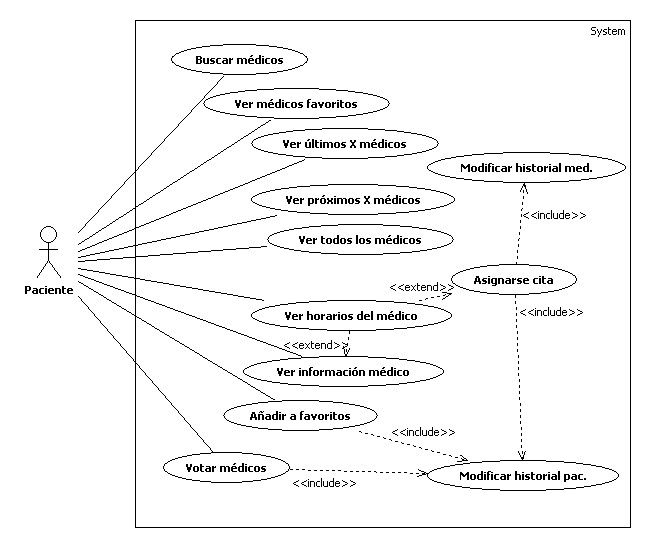
\includegraphics[width=14cm]{img/jpg/casos_uso/Gestion_medicos.jpg}
				  \caption{Gestión de médicos del paciente.}
				  \label{fig:med_pac}
				\end{figure}
				
				\begin{figure}[H]
				  \centering
				    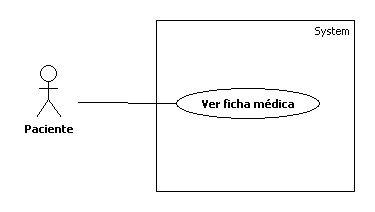
\includegraphics[width=10cm]{img/jpg/casos_uso/Ver_ficha_medica.jpg}
				  \caption{Ver ficha médica del paciente.}
				  \label{fig:ficha_pac}
				\end{figure}
			% paragraph ficha_médica (end)
			
			\paragraph{Panel de configuración del paciente} % (fold)
			\label{par:panel_de_configuracion_del_paciente}
				Un paciente tiene acceso a un panel de configuración (Figura \ref{fig:config_pac}) desde el cual modificar los datos personales (Figura \ref{fig:datos_pac}), modificar los datos de su cuenta (Figura \ref{fig:cuenta_pac}) y establecer las notificaciones que recibirá en función de diversos sucesos. Respecto a los datos, cabe destacar que podrá adjuntar o modificar una foto de su perfil. Respecto a la cuenta, que podrá cambiar su contraseña, su email, el idioma y darse de baja en el servicio cuando lo desee.
				
				Siempre que se modifiquen sus datos o la información de su cuenta, se almacerá la acción realizada en un historial del paciente, que contendrá toda la información relevante de la que pueda ser interesante mantener un registro.
				
				\begin{figure}[H]
				  \centering
				    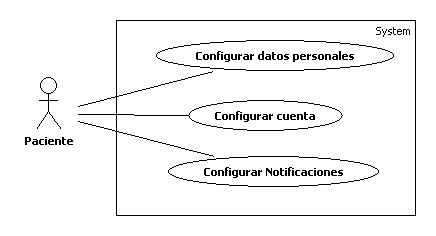
\includegraphics[width=10cm]{img/jpg/casos_uso/Configuracion_pacientes.jpg}
				  \caption{Panel de configuración del paciente.}
				  \label{fig:config_pac}
				\end{figure}
				
				\begin{figure}[H]
				  \centering
				    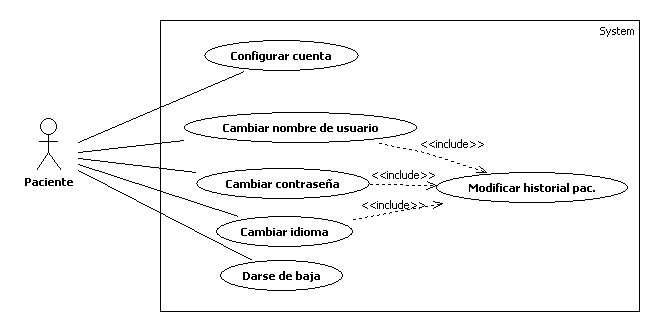
\includegraphics[width=14cm]{img/jpg/casos_uso/Cuenta.jpg}
				  \caption{Configuración de cuenta del paciente.}
				  \label{fig:cuenta_pac}
				\end{figure}
				
				\begin{figure}[H]
				  \centering
				    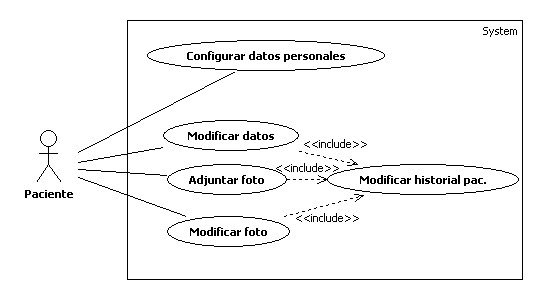
\includegraphics[width=12cm]{img/jpg/casos_uso/Datos.jpg}
				  \caption{Configuración de datos del paciente.}
				  \label{fig:datos_pac}
				\end{figure}
			% paragraph panel_de_configuración_del_paciente (end)
			
		
		% section actividades_de_los_pacientes (end)
	
		\subsection{Gestión de fichas médicas} % (fold)
		\label{sec:gestion_de_fichas_medicas}
			
			Los diagramas pretenden abarcar todo lo que un usuario registrado, tanto médico como paciente, podrá realizar con las fichas médicas.
			\paragraph{Información Personal} % (fold)
			\label{par:informacion_personal}
				Se muestra la información personal del paciente (Figura \ref{fig:infpers_fic}). Se podrán modificar los datos y adjuntar o modificar la foto del perfil.
				\begin{figure}[H]
				  \centering
				    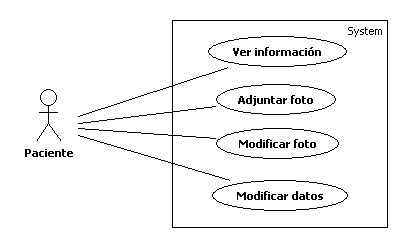
\includegraphics[width=11cm]{img/jpg/casos_uso/Informacion_personal.jpg}
				  \caption{Ficha médica. Información Personal.}
				  \label{fig:infpers_fic}
				\end{figure}
			% paragraph información_personal (end)
		
			\paragraph{Antecedentes} % (fold)
			\label{par:antecedentes}
				(Figura \ref{fig:ant_fic}) Los antecedentes de un paciente pueden ser de tres tipos, \textit{fisiológicos, familiares o personales}. Se podrán añadir o modificar antecedentes (quedará registrado en el historial de la ficha médica), y en futuras versiones, imprimir y exportar antecedentes también será una funcionalidad disponible.
				\begin{figure}[H]
				  \centering
				    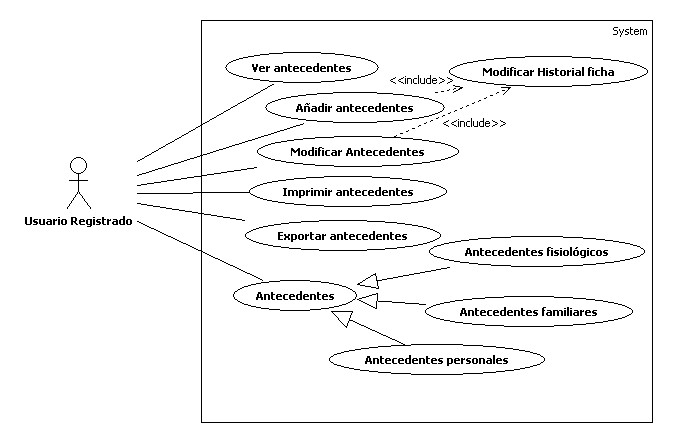
\includegraphics[width=14cm]{img/jpg/casos_uso/Antecedentes.jpg}
				  \caption{Ficha médica. Antecedentes.}
				  \label{fig:ant_fic}
				\end{figure}
			% paragraph antecedentes (end)
			
			\paragraph{Exploración} % (fold)
			\label{par:exploracion}
				(Figura \ref{fig:exp_fic}) Siempre que se añada o se modifique una exploración se modificará el historial de la ficha médica. Además, en futuras versiones se podrán imprimir y exportar las exploraciones.
				\begin{figure}[H]
				  \centering
				    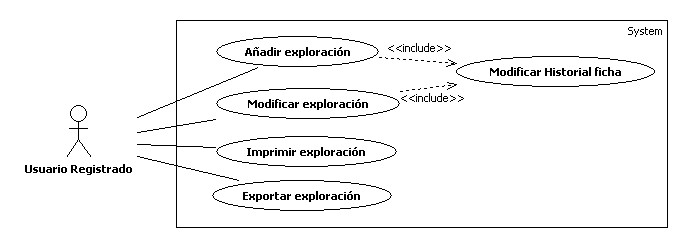
\includegraphics[width=14cm]{img/jpg/casos_uso/Exploracion.jpg}
				  \caption{Ficha médica. Exploración}
				  \label{fig:exp_fic}
				\end{figure}
			% paragraph exploración (end)
			
			\paragraph{Diagnósticos} % (fold)
				(Figura \ref{fig:diag_fic}) Cuando se añada o se modifique un diagnóstico, se modificará el historial de la ficha. Se podrá ver una lista con todos los diagnósticos y ver cada uno de ellos de manera más detallada(el último se ve así por defecto). Podrán imprimirse y exportarse.
			\label{par:diagnosticos}
				\begin{figure}[H]
				  \centering
				    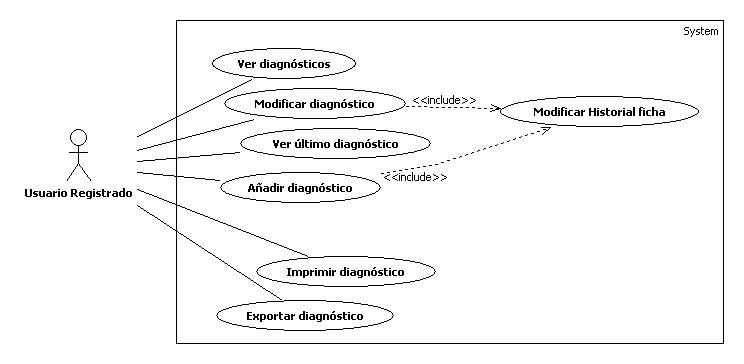
\includegraphics[width=14cm]{img/jpg/casos_uso/Diagnosticos.jpg}
				  \caption{Ficha médica. Diagnóstico.}
				  \label{fig:diag_fic}
				\end{figure}
			% paragraph diagnósticos (end)
			
			\paragraph{Tratamientos} % (fold)
			\label{par:tratamientos}
			(Figura \ref{fig:trat_fic}) Siempre que se añada o se modifique un tratamiento, se modificará el historial de la ficha médica. Se podrá ver una lista con todos los tratamientos anteriores y de forma más específica el tratamiento actual. Podrán imprimirse y exportarse.
				\begin{figure}[H]
				  \centering
				    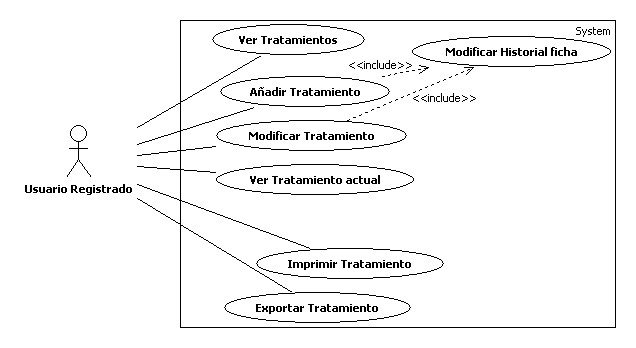
\includegraphics[width=13cm]{img/jpg/casos_uso/Tratamientos.jpg}
				  \caption{Ficha médica. Tratamiento.}
				  \label{fig:trat_fic}
				\end{figure}
			% paragraph tratamientos (end)
			
			\paragraph{Informes} % (fold)
			\label{par:informes}
				(Figura \ref{fig:inf_fic}) Siempre que se añada o se modifique un informe, se modificará el historial de la ficha médica. Se podrá ver una lista con todos los informes y ver cada uno de ellos de manera más detallada(el último se ve así por defecto). Podrán imprimirse y exportarse.
				\begin{figure}[H]
				  \centering
				    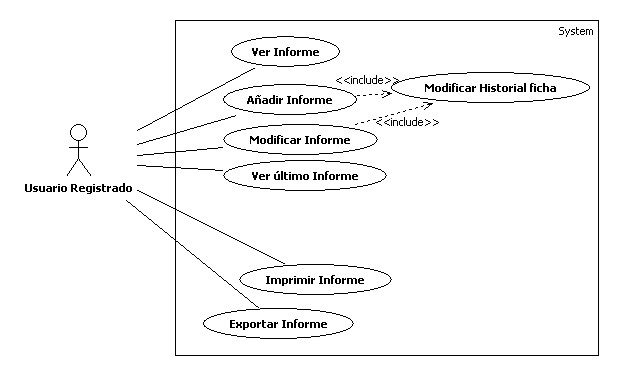
\includegraphics[width=14cm]{img/jpg/casos_uso/Informes.jpg}
				  \caption{Ficha médica. Informes.}
				  \label{fig:inf_fic}
				\end{figure}
			% paragraph informes (end)
			
			\paragraph{Observaciones} % (fold)
			\label{par:observaciones}
				(Figura \ref{fig:obs_fic}) Sólo accesible por el médico. Permite a éste ver, añadir o modificar las observaciones sobre un paciente. Las dos últimas funcionalidades modificarán, además, el historial de la ficha médica.
				\begin{figure}[H]
				  \centering
				    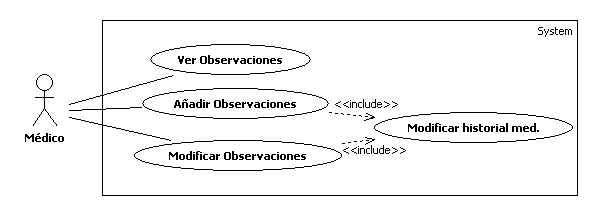
\includegraphics[width=14cm]{img/jpg/casos_uso/Observaciones.jpg}
				  \caption{Ficha médica. Observaciones.}
				  \label{fig:obs_fic}
				\end{figure}
			% paragraph observaciones (end)
			
			\paragraph{Historial de la ficha} % (fold)
			\label{par:historial_de_la_ficha}
				En el historial de la ficha médica se almacena toda la información que pueda resultar relevante cada vez que una acción en la aplicación realice una función sobre la información que contiene. Además, éstas acciones en las que se añada o modifique información importante, también quedarán registradas en la ficha del médico y en la ficha del paciente. Se podrán realizar búsquedas mediante diversos filtros en el historial de las fichas. Podrá imprimirse y exportarse. (Figura \ref{fig:hist_fic}).
				\begin{figure}[H]
				  \centering
				    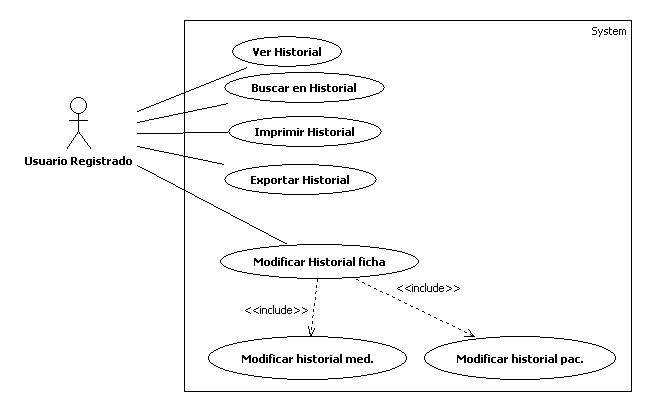
\includegraphics[width=14cm]{img/jpg/casos_uso/Historial_ficha.jpg}
				  \caption{Ficha médica. Historial de la Ficha.}
				  \label{fig:hist_fic}
				\end{figure}
			% paragraph historial_de_la_ficha (end)
			
			\paragraph{Pruebas} % (fold
			
				(Figura \ref{fig:pruebas_gestion_fic}) Se podrán ver pruebas y añadirlas (al insertar una nueva prueba en la aplicación, se modifica el historial de la ficha médica). El actor médico es el único que puede solicitar una nueva prueba. Podrán imprimirse y exportarse.
				
				Se pueden ver distintos tipos de pruebas (Figura \ref{fig:pruebas_ver_fic}) relacionadas con cada una de las posibles especialidades. Lo mismo ocurre con la opción de añadir pruebas (Figura \ref{fig:pruebas_add_fic}) y de solicitar pruebas (Figura \ref{fig:pruebas_sol_fic}). Sin embargo, esta última acción sólo podrán realizarla los actores médicos.
				
			\fbox{\parbox{15cm}{En una primera iteración, la aplicación se centrará sólo en las pruebas radiodiagnósticas y en los análisis.}}	
				
			\label{par:pruebas}
				\begin{figure}[H]
				  \centering
				    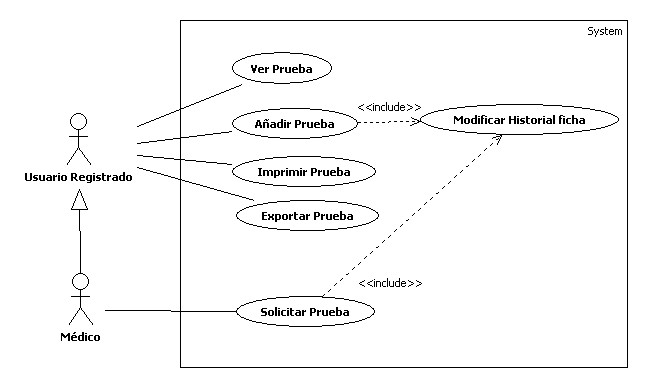
\includegraphics[width=13cm]{img/jpg/casos_uso/Gestion_pruebas.jpg}
				  \caption{Ficha médica. Pruebas. Gestión de Pruebas.}
				  \label{fig:pruebas_gestion_fic}
				\end{figure}
				
				\begin{figure}[H]
				  \centering
				    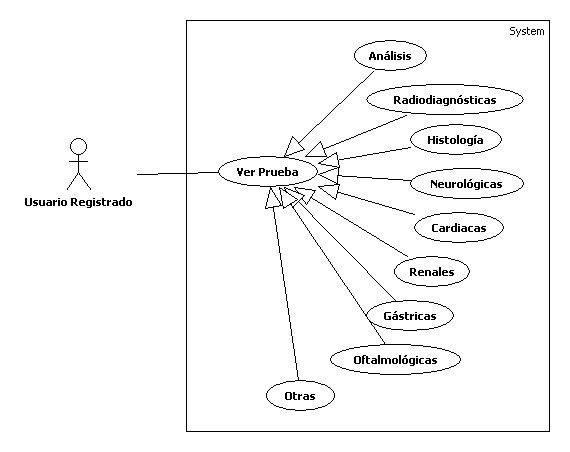
\includegraphics[width=10cm]{img/jpg/casos_uso/Ver_Prueba.jpg}
				  \caption{Ficha médica. Pruebas. Ver Prueba.}
				  \label{fig:pruebas_ver_fic}
				\end{figure}
				
				\begin{figure}[H]
				  \centering
				    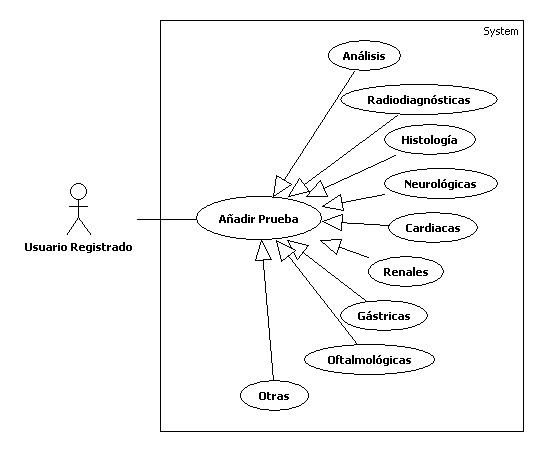
\includegraphics[width=10cm]{img/jpg/casos_uso/Add_Prueba.jpg}
				  \caption{Ficha médica. Pruebas. Añadir Prueba.}
				  \label{fig:pruebas_add_fic}
				\end{figure}
				
				\begin{figure}[H]
				  \centering
				    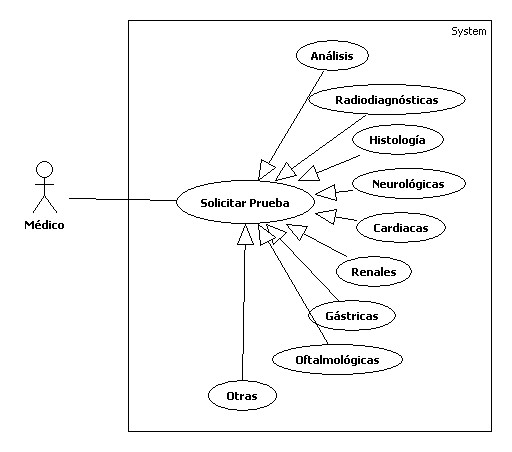
\includegraphics[width=10cm]{img/jpg/casos_uso/Solicitar_Prueba.jpg}
				  \caption{Ficha médica. Pruebas. Solicitar prueba.}
				  \label{fig:pruebas_sol_fic}
				\end{figure}
			% paragraph pruebas (end)
			
		% section gestión_de_fichas_médicas (end)
	
		\subsection{Panel del Administrador} % (fold)
		\label{sec:panel_del_administrador}
		
			El actor Administrador del sistema tiene una seria de funciones importantes relativas a la aplicación. 
			
			Entre ellas cabe destacar la de \textit{verificar médicos}, con la cuál da de alta a un médico en el sistema haciéndolo visible para el resto de usuarios de la aplicación. Operaciones similares son las de \textit{eliminar médicos, suspender médicos o reactivar médicos}. 
			
			Otras funciones son las de \textit{ver, contestar y eliminar} las preguntas de los usuarios. También podrá modificar fácilmente \textit{las condiciones de uso, los datos de contacto y los términos legales}. 
			
			Por último, podrá \textit{agregar a otro administrador}.
			
			\begin{figure}[H]
			  \centering
			    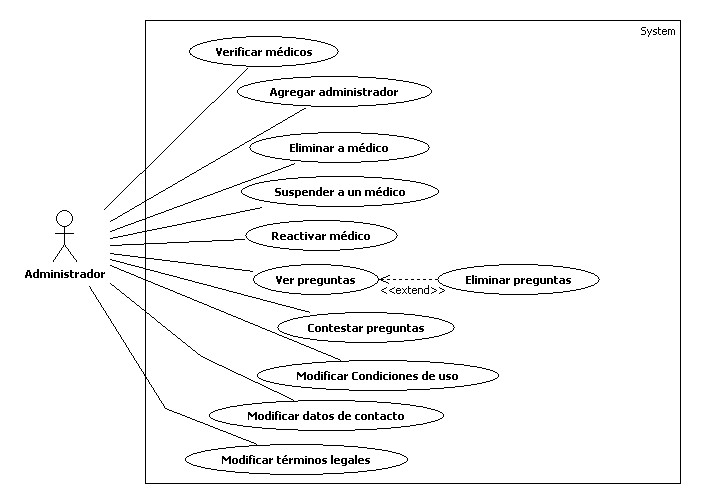
\includegraphics[width=15cm]{img/jpg/casos_uso/Panel_de_Administrador.jpg}
			  \caption{Panel del Administrador.}
			  \label{fig:panel_admin}
			\end{figure}
					
		% section panel_del_administrador (end)
	
	% subsection diagramas_de_casos_de_uso (end)
	\newpage
	\section{Descripción formal de los Casos de Uso} % (fold)
	\label{sub:descripcion_formal_de_los_casos_de_uso}
		
		La especificación de un caso de uso debe describir el modo en que un actor interactúa con el sistema. Es mucho más importante que los diagramas, de hecho, el 90 por ciento del contenido de los casos de uso está en dichas descripciones.
			
		\subsection{Estructura de la descripción} % (fold)
		\label{sub:estructura_de_la_descripcion}
		
			Para realizar la descripción formal de los casos de uso se van a utilizar unas tablas en las que se pretende abarcar toda la información necesaria para realizar dicha tarea. Los campos empleados serán los siguientes.
		
			\begin{itemize}
				\item \textbf{Identificador}. Cada caso de uso tendrá un ID único. La estructura será \textit{Categoría} + Número del caso de uso. Las categorías se agrupan de forma jerárquica en seis grandes grupos.
					\begin{itemize}
						\item \textit{ACT}. Actores.
						\item \textit{GAG}. Gestión de Actividades generales.
						\item \textit{GAM}. Gestión de Actividades de los médicos.
						\item \textit{GAP}. Gestión de Actividades de los pacientes.
						\item \textit{GFM}. Gestión de las Fichas médicas.
						\item \textit{GPA}. Gestión del Panel del Administrador.
					\end{itemize}
				
				\item \textbf{Nombre}. Todo caso de uso tendrá un nombre que refleja las tareas y funcionalidades que el usuario podrá llevar a cabo. Suele estar formado por un verbo que ejecute una acción y un sustantivo.

				\item \textbf{Historial}. Tiene los siguientes apartados.
					\begin{itemize}
						\item \textit{Fecha de creación}. Fecha en la que se documentó el caso de uso.
						\item \textit{Fecha de la última actualización}. Fecha en la que se realizó la última modificación en la descripción del caso de uso.
					\end{itemize}
					
				\item \textbf{Actores}. El nombre del actor que inició este caso de uso y cualquier otro actor que participe en su realización.  
			
				\item \textbf{Descripción}. Proporciona una breve descripción del caso de uso.
				
				\item \textbf{Precondición}. Describe lo que se sabe que es verdadero antes de que inicie el caso de uso. 
				
				\item \textbf{Postcondición}. Describe el estado del sistema al finalizar la ejecución del caso de uso.
				
				\item \textbf{Camino normal}. Proporcionar una descripción detallada de las acciones del usuario y las respuestas del sistema que se llevarán a cabo durante la ejecución del caso de uso en condiciones normales, es decir, si todo sucede como se esperaba. Esta secuencia de diálogo pretende alcanzar, en última instancia, el objetivo expuesto en el nombre y la descripción de casos de uso. Se hará mediante una lista numerada de las acciones realizadas por el actor, alternando con las respuestas proporcionadas por el sistema.
				
				\item \textbf{Camino alternativo}. Es un flujo alternativo al del camino normal, con diferencias en la secuencia de pasos que tienen lugar. 
				
				\item \textbf{Include}. Lista de otros casos de uso que se incluyen en éste. Funcionalidad común que aparece en múltiples casos de uso.
				
				\item \textbf{Extends}. 
				
				\item \textbf{Iteración}. Indica si el caso de uso se realizará en esta versión o en versiones posteriores.
		
			\end{itemize}
		
		% subsection estructura_de_la_descripción (end)
		
		\subsection{Descripción de los casos de uso} % (fold)
		\label{sub:descripcion_de_los_casos_de_uso}
		
			\subsubsection{Actores} % (fold)
			\label{sub:actores}
				Encontramos cinco tipos de actores.
				\begin{itemize}
					\item \textit{Usuario Genérico}. Un usuario genérico es aquel que puede acceder a secciones del servicio para las que no es necesario estar registrado, como por ejemplo, ver preguntas frecuentes, realizar un tour por la aplicación o ver si algún médico está en el sistema. Podrá darse de alta en cualquier momento que lo desee, tanto con el rol de médico cómo con el de paciente.
					\item \textit{Usuario Registrado}. Puede ser un médico o un paciente. A ellos está destinada la aplicación.
						\begin{itemize}
							\item \textit{Médico}. Un usuario médico es aquel que se ha identificado cómo tal. Realizará funciones propias de los médicos. La aplicación está destinada a ellos principalmente.
							\item \textit{Paciente}. Un usuario paciente es aquel que accede a la aplicación en busca de un médico. Sus funcionalidades están más limitadas.
						\end{itemize}
					\item \textit{Usuario Administrador}. Un usuario Administrador es el encargado de gestionar temas concernientes a la aplicación. Será el que se encargue de dar de alta a los médicos que contraten el servicio, de contestar a las preguntas de los usuarios, etcétera. No utilizará ninguna funcionalidad de las destinadas a médicos y pacientes.
					 
				\end{itemize}
			% paragraph actores (end)
			\newpage
			\subsubsection{Actividades Generales (GAG)} % (fold)
			\label{sub:actividades_generales_gag_}
			
				Una serie de acciones y funciones que pueden desarrollar los usuarios sin necesidad de estar registrados en el sistema. Además, lo referente al acceso y la autentificación por parte de usuarios registrados.
				\bigskip
			
				
				% Registrarse
				\begin{tabular}{|l|p{4cm}|p{4cm}|p{4cm}|}\hline
					\multicolumn{1}{|>{\columncolor{gris2}}l|}{Identificador} & \multicolumn{3}{|p{12cm}|}{GAG-01 (Figura \ref{fig:reg_inf})}	\\\hline
					\multicolumn{1}{|>{\columncolor{gris2}}l|}{Nombre} & \multicolumn{3}{|p{12cm}|}{Registrarse} \\\hline
					\multicolumn{1}{|>{\columncolor{gris2}}l|}{Fecha de creación} & 05/04/2011 & \multicolumn{1}{|>{\columncolor{gris2}}l|}{Fecha de actualización} & --- \\\hline
					\multicolumn{1}{|>{\columncolor{gris2}}l|}{Actor}  & \multicolumn{3}{|p{12cm}|}{Usuario Genérico} 	\\\hline			
					\multicolumn{4}{|>{\columncolor{gris2}}l|}{Descripción} \\\hline
					\multicolumn{4}{|p{16cm}|}{Un usuario genérico puede registrarse en el sistema. Cuando se registra, debe rellenar su información personal. Puede registrarse con el rol de médico o con el de paciente. En función del tipo de rol que vaya a desempeñar, el usuario que se registre deberá rellenar distinta información.}	\\\hline
					\multicolumn{1}{|>{\columncolor{gris2}}l|}{Precondición} & \multicolumn{3}{|p{12cm}|}{Que el usuario genérico esté en la página de registro.} \\\hline
					\multicolumn{4}{|>{\columncolor{gris2}}l|}{Camino normal} \\\hline
					\multicolumn{4}{|p{16cm}|}{Caso de uso abstracto}	\\\hline
					\multicolumn{4}{|>{\columncolor{gris2}}l|}{Camino alternativo} \\\hline
					\multicolumn{4}{|p{16cm}|}{---}	\\\hline
					\multicolumn{1}{|>{\columncolor{gris2}}l|}{Postcondición} & \multicolumn{3}{|p{12cm}|}{Se guardan los datos en la base de datos y el usuario puede ingresar al sistema.}  \\\hline
					\multicolumn{1}{|>{\columncolor{gris2}}l|}{Include} & \multicolumn{3}{|p{12cm}|}{---}  \\\hline
					\multicolumn{1}{|>{\columncolor{gris2}}l|}{Extend} & \multicolumn{3}{|p{12cm}|}{---}  \\\hline
					\multicolumn{1}{|>{\columncolor{gris2}}l|}{Iteración} & \multicolumn{3}{|p{12cm}|}{Primera}  \\\hline			
				\end{tabular}  \bigskip \bigskip
				
				% Registrarse como paciente
				\begin{tabular}{|l|p{4cm}|p{4cm}|p{4cm}|}\hline
					\multicolumn{1}{|>{\columncolor{gris2}}l|}{Identificador} & \multicolumn{3}{|p{12cm}|}{GAG-02 (Figura \ref{fig:reg_inf})}	\\\hline
					\multicolumn{1}{|>{\columncolor{gris2}}l|}{Nombre} & \multicolumn{3}{|p{12cm}|}{Registrarse cómo paciente} \\\hline
					\multicolumn{1}{|>{\columncolor{gris2}}l|}{Fecha de creación} & 05/04/2011 & \multicolumn{1}{|>{\columncolor{gris2}}l|}{Fecha de actualización} & 11/04/2011 \\\hline
					\multicolumn{1}{|>{\columncolor{gris2}}l|}{Actor}  & \multicolumn{3}{|p{12cm}|}{Usuario Genérico} 	\\\hline			
					\multicolumn{4}{|>{\columncolor{gris2}}l|}{Descripción} \\\hline
					\multicolumn{4}{|p{16cm}|}{Un usuario puede registrarse como paciente.}	\\\hline
					\multicolumn{1}{|>{\columncolor{gris2}}l|}{Precondición} & \multicolumn{3}{|p{12cm}|}{Que el usuario esté en la página de registro de pacientes.} \\\hline
					
					\multicolumn{4}{|>{\columncolor{gris2}}l|}{Camino normal} \\\hline
						\multicolumn{4}{|p{16cm}|}{1.- Hacer click en Registrar como paciente.} \\
						\multicolumn{4}{|p{16cm}|}{2.- Ingresar el email.} \\
						\multicolumn{4}{|p{16cm}|}{3.- El software valida que el email sea válido.} \\
						\multicolumn{4}{|p{16cm}|}{4.- Ingresar el nombre de usuario.} \\
						\multicolumn{4}{|p{16cm}|}{5.- El software valida que el nombre de usuario está disponible.} \\
						\multicolumn{4}{|p{16cm}|}{6.- Ingresar contraseña} \\
						\multicolumn{4}{|p{16cm}|}{7.- Confirmar contraseña.} \\
						\multicolumn{4}{|p{16cm}|}{8.- Darle al botón de aceptar.} \\
						\multicolumn{4}{|p{16cm}|}{9.- El software valida que la contraseña coincide y que es fuerte.} \\
						\multicolumn{4}{|p{16cm}|}{10.- El software permite que el usuario se registre.} \\
						\multicolumn{4}{|p{16cm}|}{11.- El paciente puede ingresar.} \\\hline
					
					\multicolumn{4}{|>{\columncolor{gris2}}l|}{Camino alternativo} \\\hline
						\multicolumn{4}{|p{16cm}|}{3.1.- El software muestra un mensaje de error si el email no es válido.} \\
						\multicolumn{4}{|p{16cm}|}{5.1.- El software muestra un mensaje de error si el nombre de usuario ya existe.} \\
						\multicolumn{4}{|p{16cm}|}{9.1.- El software muestra un mensaje de error si la contraseña no coincide.} \\\hline

					\multicolumn{1}{|>{\columncolor{gris2}}l|}{Postcondición} & \multicolumn{3}{|p{12cm}|}{Se guardan los datos en la base de datos y el paciente puede ingresar al sistema.}  \\\hline
					\multicolumn{1}{|>{\columncolor{gris2}}l|}{Include} & \multicolumn{3}{|p{12cm}|}{---}  \\\hline
					\multicolumn{1}{|>{\columncolor{gris2}}l|}{Extend} & \multicolumn{3}{|p{12cm}|}{---}  \\\hline
					\multicolumn{1}{|>{\columncolor{gris2}}l|}{Iteración} & \multicolumn{3}{|p{12cm}|}{Primera}  \\\hline			
				\end{tabular}  \bigskip \bigskip
				
				% Registrarse como médico
				\begin{tabular}{|l|p{4cm}|p{4cm}|p{4cm}|}\hline
					\multicolumn{1}{|>{\columncolor{gris2}}l|}{Identificador} & \multicolumn{3}{|p{12cm}|}{GAG-03 (Figura \ref{fig:reg_inf})}	\\\hline
					\multicolumn{1}{|>{\columncolor{gris2}}l|}{Nombre} & \multicolumn{3}{|p{12cm}|}{Registrarse cómo médico} \\\hline
					\multicolumn{1}{|>{\columncolor{gris2}}l|}{Fecha de creación} & 05/04/2011 & \multicolumn{1}{|>{\columncolor{gris2}}l|}{Fecha de actualización} & 11/04/2011 \\\hline
					\multicolumn{1}{|>{\columncolor{gris2}}l|}{Actor}  & \multicolumn{3}{|p{12cm}|}{Usuario Genérico} 	\\\hline			
					\multicolumn{4}{|>{\columncolor{gris2}}l|}{Descripción} \\\hline
					\multicolumn{4}{|p{16cm}|}{Un usuario puede registrarse cómo médico, lo cuál incluirá una serie de preguntas adicionales relacionadas con su consulta, especialidad, etcétera.}	\\\hline
					\multicolumn{1}{|>{\columncolor{gris2}}l|}{Precondición} & \multicolumn{3}{|p{12cm}|}{Que el usuario esté en la página de registro de médicos.} \\\hline
					\multicolumn{4}{|>{\columncolor{gris2}}l|}{Camino normal} \\\hline
						\multicolumn{4}{|p{16cm}|}{1.- Hacer click en Registrar como médico.} \\
						\multicolumn{4}{|p{16cm}|}{2.- Ingresar el email.} \\
						\multicolumn{4}{|p{16cm}|}{3.- El software valida que el email sea válido.} \\
						\multicolumn{4}{|p{16cm}|}{4.- Ingresar el nombre de usuario.} \\
						\multicolumn{4}{|p{16cm}|}{5.- El software valida que el nombre de usuario está disponible.} \\
						\multicolumn{4}{|p{16cm}|}{6.- Ingresar la especialidad entre las disponibles en una lista.} \\
						\multicolumn{4}{|p{16cm}|}{7.- Ingresar contraseña} \\
						\multicolumn{4}{|p{16cm}|}{8.- Confirmar contraseña.} \\
						\multicolumn{4}{|p{16cm}|}{9.- Darle al botón de aceptar.} \\
						\multicolumn{4}{|p{16cm}|}{10.- El software valida que la contraseña coincide y que es fuerte.} \\
						\multicolumn{4}{|p{16cm}|}{11.- El software permite que el usuario se registre.} \\
						\multicolumn{4}{|p{16cm}|}{12.- El médico puede ingresar.} \\\hline
					
					\multicolumn{4}{|>{\columncolor{gris2}}l|}{Camino alternativo} \\\hline
						\multicolumn{4}{|p{16cm}|}{3.1.- El software muestra un mensaje de error si el email no es válido.} \\
						\multicolumn{4}{|p{16cm}|}{5.1.- El software muestra un mensaje de error si el nombre de usuario ya existe.} \\
						\multicolumn{4}{|p{16cm}|}{9.1.- El software muestra un mensaje de error si la contraseña no coincide.} \\\hline

					\multicolumn{1}{|>{\columncolor{gris2}}l|}{Postcondición} & \multicolumn{3}{|p{12cm}|}{Se guardan los datos en la base de datos y el médico puede ingresar al sistema.}  \\\hline
					\multicolumn{1}{|>{\columncolor{gris2}}l|}{Include} & \multicolumn{3}{|p{12cm}|}{---}  \\\hline
					\multicolumn{1}{|>{\columncolor{gris2}}l|}{Extend} & \multicolumn{3}{|p{12cm}|}{---}  \\\hline
					\multicolumn{1}{|>{\columncolor{gris2}}l|}{Iteración} & \multicolumn{3}{|p{12cm}|}{Primera}  \\\hline			
				\end{tabular}  \bigskip \bigskip
				
				% Rellenar información personal
				\begin{tabular}{|l|p{4cm}|p{4cm}|p{4cm}|}\hline
					\multicolumn{1}{|>{\columncolor{gris2}}l|}{Identificador} & \multicolumn{3}{|p{12cm}|}{GAG-04 (Figura \ref{fig:reg_inf})}	\\\hline
					\multicolumn{1}{|>{\columncolor{gris2}}l|}{Nombre} & \multicolumn{3}{|p{12cm}|}{Rellenar información personal} \\\hline
					\multicolumn{1}{|>{\columncolor{gris2}}l|}{Fecha de creación} & 05/04/2011 & \multicolumn{1}{|>{\columncolor{gris2}}l|}{Fecha de actualización} & 11/04/2011 \\\hline
					\multicolumn{1}{|>{\columncolor{gris2}}l|}{Actor}  & \multicolumn{3}{|p{12cm}|}{Usuario Registrado} 	\\\hline			
					\multicolumn{4}{|>{\columncolor{gris2}}l|}{Descripción} \\\hline
					\multicolumn{4}{|p{16cm}|}{Un usuario debe rellenar toda su información personal después del registro. Además, si lo desea, puede adjuntar la foto de su perfil.}	\\\hline
					\multicolumn{1}{|>{\columncolor{gris2}}l|}{Precondición} & \multicolumn{3}{|p{12cm}|}{El usuario debe estar registrado y acceder por primera vez al sistema o estar en el panel de configuración de datos.} \\\hline					
					\multicolumn{4}{|>{\columncolor{gris2}}l|}{Camino normal} \\\hline
						\multicolumn{4}{|p{16cm}|}{1.- Ingresar Nombre y apellidos.} \\
						\multicolumn{4}{|p{16cm}|}{2.- Ingresar DNI.} \\
						\multicolumn{4}{|p{16cm}|}{3.- El software valida que el DNI sea válido.} \\
						\multicolumn{4}{|p{16cm}|}{4.- Ingresar el teléfono de contacto.} \\
						\multicolumn{4}{|p{16cm}|}{5.- Ingresar dirección.} \\
						\multicolumn{4}{|p{16cm}|}{6.- Si lo desea, adjuntar una foto para el perfil.} \\
						\multicolumn{4}{|p{16cm}|}{7.- Hacer click en guardar cambios.} \\
						\multicolumn{4}{|p{16cm}|}{8.- El software almacena los datos introducidos.} \\
						\multicolumn{4}{|p{16cm}|}{9.- Los datos podrán ser modificados en el futuro.}\\\hline
					
					\multicolumn{4}{|>{\columncolor{gris2}}l|}{Camino alternativo} \\\hline
						\multicolumn{4}{|p{16cm}|}{3.1.- El software muestra un mensaje de error si el DNI no es válido.} \\
						\multicolumn{4}{|p{16cm}|}{6.1.- El software muestra un mensaje de error si existió algún problema al almacenar la imagen.} \\
						\multicolumn{4}{|p{16cm}|}{8.1.- El software muestra un mensaje de error si se produjo algún fallo con la base de datos.} \\\hline
						
					\multicolumn{1}{|>{\columncolor{gris2}}l|}{Postcondición} & \multicolumn{3}{|p{12cm}|}{Los datos del usuario estarán almacenados en la BD y podrán ser modificados en el futuro.}  \\\hline
					\multicolumn{1}{|>{\columncolor{gris2}}l|}{Include} & \multicolumn{3}{|p{12cm}|}{---}  \\\hline
					\multicolumn{1}{|>{\columncolor{gris2}}l|}{Extend} & \multicolumn{3}{|p{12cm}|}{Adjuntar foto de perfil (GAG-06)}  \\\hline
					\multicolumn{1}{|>{\columncolor{gris2}}l|}{Iteración} & \multicolumn{3}{|p{12cm}|}{Primera}  \\\hline			
				\end{tabular}  \bigskip \bigskip
				
				% Rellenar información de la consulta
				\begin{tabular}{|l|p{4cm}|p{4cm}|p{4cm}|}\hline
					\multicolumn{1}{|>{\columncolor{gris2}}l|}{Identificador} & \multicolumn{3}{|p{12cm}|}{GAG-05 (Figura \ref{fig:reg_inf})}	\\\hline
					\multicolumn{1}{|>{\columncolor{gris2}}l|}{Nombre} & \multicolumn{3}{|p{12cm}|}{Rellenar información de la consulta médica} \\\hline
					\multicolumn{1}{|>{\columncolor{gris2}}l|}{Fecha de creación} & 05/04/2011 & \multicolumn{1}{|>{\columncolor{gris2}}l|}{Fecha de actualización} & 11/04/2011 \\\hline
					\multicolumn{1}{|>{\columncolor{gris2}}l|}{Actor}  & \multicolumn{3}{|p{12cm}|}{Médico} 	\\\hline			
					\multicolumn{4}{|>{\columncolor{gris2}}l|}{Descripción} \\\hline
					\multicolumn{4}{|p{16cm}|}{Un médico debe rellenar todos todos los datos referentes a la localización y el contacto de su consulta médica una vez se ha registrado.}	\\\hline
					\multicolumn{1}{|>{\columncolor{gris2}}l|}{Precondición} & \multicolumn{3}{|p{12cm}|}{El médico debe estar registrado como médico y acceder por primera vez al sistema o estar en el panel de configuración de datos de la consulta.} \\\hline							
					\multicolumn{4}{|>{\columncolor{gris2}}l|}{Camino normal} \\\hline
						\multicolumn{4}{|p{16cm}|}{1.- Ingresar Nombre del centro.} \\
						\multicolumn{4}{|p{16cm}|}{2.- Ingresar CIF.} \\
						\multicolumn{4}{|p{16cm}|}{3.- Ingresar datos de localización.} \\
						\multicolumn{4}{|p{16cm}|}{4.- Ingresar datos de contacto} \\
						\multicolumn{4}{|p{16cm}|}{5.- Si lo desea, puede adjuntar o crear un curriculum.} \\
						\multicolumn{4}{|p{16cm}|}{6.- Ingresar el número de cuenta en el que se realizarán los ingresos.} \\
						\multicolumn{4}{|p{16cm}|}{7.- Hacer click en guardar cambios.} \\
						\multicolumn{4}{|p{16cm}|}{8.- El software almacena los datos introducidos.} \\
						\multicolumn{4}{|p{16cm}|}{9.- Los datos podrán ser modificados en el futuro.}\\\hline
					
					\multicolumn{4}{|>{\columncolor{gris2}}l|}{Camino alternativo} \\\hline
						\multicolumn{4}{|p{16cm}|}{5.1.- El software muestra un mensaje de error si existió algún problema al adjuntar o crear un curriculum.} \\
						\multicolumn{4}{|p{16cm}|}{8.1.- El software muestra un mensaje de error si se produjo algún fallo con la base de datos.} \\\hline
											
					\multicolumn{1}{|>{\columncolor{gris2}}l|}{Postcondición} & \multicolumn{3}{|p{12cm}|}{Los datos de la consulta del médico estarán almacenados en la BD y podrán ser modificados en el futuro.}  \\\hline
					\multicolumn{1}{|>{\columncolor{gris2}}l|}{Include} & \multicolumn{3}{|p{12cm}|}{---}  \\\hline
					\multicolumn{1}{|>{\columncolor{gris2}}l|}{Extend} & \multicolumn{3}{|p{12cm}|}{Adjuntar curriculum(GAM-13), Crear curriculum(GAM-15)}  \\\hline
					\multicolumn{1}{|>{\columncolor{gris2}}l|}{Iteración} & \multicolumn{3}{|p{12cm}|}{Primera}  \\\hline			
				\end{tabular}  \bigskip \bigskip
				
				% Adjuntar foto del perfil
				\begin{tabular}{|l|p{4cm}|p{4cm}|p{4cm}|}\hline
					\multicolumn{1}{|>{\columncolor{gris2}}l|}{Identificador} & \multicolumn{3}{|p{12cm}|}{GAG-06 (Figura \ref{fig:reg_inf})}	\\\hline
					\multicolumn{1}{|>{\columncolor{gris2}}l|}{Nombre} & \multicolumn{3}{|p{12cm}|}{Adjuntar foto del perfil} \\\hline
					\multicolumn{1}{|>{\columncolor{gris2}}l|}{Fecha de creación} & 05/04/2011 & \multicolumn{1}{|>{\columncolor{gris2}}l|}{Fecha de actualización} & --- \\\hline
					\multicolumn{1}{|>{\columncolor{gris2}}l|}{Actor}  & \multicolumn{3}{|p{12cm}|}{Usuario Registrado} 	\\\hline			
					\multicolumn{4}{|>{\columncolor{gris2}}l|}{Descripción} \\\hline
					\multicolumn{4}{|p{16cm}|}{Permite adjuntar  una foto de perfil para que sea vista por otros usuarios.}	\\\hline
					\multicolumn{1}{|>{\columncolor{gris2}}l|}{Precondición} & \multicolumn{3}{|p{12cm}|}{Estar registrado y en las pantallas de rellenar información o de modificar datos.} \\\hline
					\multicolumn{4}{|>{\columncolor{gris2}}l|}{Camino normal} \\\hline
					\multicolumn{4}{|p{16cm}|}{---}	\\\hline
					\multicolumn{4}{|>{\columncolor{gris2}}l|}{Camino alternativo} \\\hline
					\multicolumn{4}{|p{16cm}|}{---}	\\\hline
					\multicolumn{1}{|>{\columncolor{gris2}}l|}{Postcondición} & \multicolumn{3}{|p{12cm}|}{El usuario tiene una foto de perfil que será visible por el resto de usuarios}  \\\hline
					\multicolumn{1}{|>{\columncolor{gris2}}l|}{Include} & \multicolumn{3}{|p{12cm}|}{---}  \\\hline
					\multicolumn{1}{|>{\columncolor{gris2}}l|}{Extend} & \multicolumn{3}{|p{12cm}|}{---}  \\\hline
					\multicolumn{1}{|>{\columncolor{gris2}}l|}{Iteración} & \multicolumn{3}{|p{12cm}|}{Segunda}  \\\hline			
				\end{tabular}  \bigskip \bigskip
				
				% Tour de la aplicación
				\begin{tabular}{|l|p{4cm}|p{4cm}|p{4cm}|}\hline
					\multicolumn{1}{|>{\columncolor{gris2}}l|}{Identificador} & \multicolumn{3}{|p{12cm}|}{GAG-07 (Figura \ref{fig:caracteristicas})}	\\\hline
					\multicolumn{1}{|>{\columncolor{gris2}}l|}{Nombre} & \multicolumn{3}{|p{12cm}|}{Realizar tour por la aplicación} \\\hline
					\multicolumn{1}{|>{\columncolor{gris2}}l|}{Fecha de creación} & 05/04/2011 & \multicolumn{1}{|>{\columncolor{gris2}}l|}{Fecha de actualización} & --- \\\hline
					\multicolumn{1}{|>{\columncolor{gris2}}l|}{Actor}  & \multicolumn{3}{|p{12cm}|}{Usuario Genérico y Usuario Registrado} 	\\\hline			
					\multicolumn{4}{|>{\columncolor{gris2}}l|}{Descripción} \\\hline
					\multicolumn{4}{|p{16cm}|}{Cualquier usuario genérico podrá hacer una visita guiada sobre las principales funcionalidades de la aplicación, tanto desde el punto de vista del médico cómo desde el punto de vista del paciente.}	\\\hline
					\multicolumn{1}{|>{\columncolor{gris2}}l|}{Precondición} & \multicolumn{3}{|p{12cm}|}{El usuario debe estar en la pantalla de Tour por la aplicación.} \\\hline
					\multicolumn{4}{|>{\columncolor{gris2}}l|}{Camino normal} \\\hline
					\multicolumn{4}{|p{16cm}|}{---}	\\\hline
					\multicolumn{4}{|>{\columncolor{gris2}}l|}{Camino alternativo} \\\hline
					\multicolumn{4}{|p{16cm}|}{---}	\\\hline
					\multicolumn{1}{|>{\columncolor{gris2}}l|}{Postcondición} & \multicolumn{3}{|p{12cm}|}{El usuario tendrá una idea de la información que le haya interesado sobre la aplicación.}  \\\hline
					\multicolumn{1}{|>{\columncolor{gris2}}l|}{Include} & \multicolumn{3}{|p{12cm}|}{---}  \\\hline
					\multicolumn{1}{|>{\columncolor{gris2}}l|}{Extend} & \multicolumn{3}{|p{12cm}|}{---}  \\\hline
					\multicolumn{1}{|>{\columncolor{gris2}}l|}{Iteración} & \multicolumn{3}{|p{12cm}|}{Segunda}  \\\hline			
				\end{tabular}  \bigskip \bigskip
				
				% Ver términos legales
				\begin{tabular}{|l|p{4cm}|p{4cm}|p{4cm}|}\hline
					\multicolumn{1}{|>{\columncolor{gris2}}l|}{Identificador} & \multicolumn{3}{|p{12cm}|}{GAG-08 (Figura \ref{fig:caracteristicas})}	\\\hline
					\multicolumn{1}{|>{\columncolor{gris2}}l|}{Nombre} & \multicolumn{3}{|p{12cm}|}{Ver términos legales} \\\hline
					\multicolumn{1}{|>{\columncolor{gris2}}l|}{Fecha de creación} & 05/04/2011 & \multicolumn{1}{|>{\columncolor{gris2}}l|}{Fecha de actualización} & 11/04/2011 \\\hline
					\multicolumn{1}{|>{\columncolor{gris2}}l|}{Actor}  & \multicolumn{3}{|p{12cm}|}{Usuario Genérico y Usuario Registrado} 	\\\hline			
					\multicolumn{4}{|>{\columncolor{gris2}}l|}{Descripción} \\\hline
					\multicolumn{4}{|p{16cm}|}{Cualquier usuario genérico ó registrado puede ver los términos legales y los detalles concernientes a la protección de datos.}	\\\hline
					\multicolumn{1}{|>{\columncolor{gris2}}l|}{Precondición} & \multicolumn{3}{|p{12cm}|}{El usuario debe hacer click en \textit{Ver términos legales}} \\\hline
					\multicolumn{4}{|>{\columncolor{gris2}}l|}{Camino normal} \\\hline
						\multicolumn{4}{|p{16cm}|}{1.- Hacer click en \textit{Ver términos legales}.} \\
						\multicolumn{4}{|p{16cm}|}{2.- Leer los términos legales.} \\
						\multicolumn{4}{|p{16cm}|}{3.- Hacer click en \textit{volver atrás}.} \\\hline
					
					\multicolumn{4}{|>{\columncolor{gris2}}l|}{Camino alternativo} \\\hline
						\multicolumn{4}{|p{16cm}|}{---} \\\hline

					\multicolumn{1}{|>{\columncolor{gris2}}l|}{Postcondición} & \multicolumn{3}{|p{12cm}|}{Se volverá a la pantalla inicial(si el usuario es genérico) o al tablero (si el usuario está registrado).}  \\\hline
					\multicolumn{1}{|>{\columncolor{gris2}}l|}{Include} & \multicolumn{3}{|p{12cm}|}{---}  \\\hline
					\multicolumn{1}{|>{\columncolor{gris2}}l|}{Extend} & \multicolumn{3}{|p{12cm}|}{---}  \\\hline
					\multicolumn{1}{|>{\columncolor{gris2}}l|}{Iteración} & \multicolumn{3}{|p{12cm}|}{Primera}  \\\hline			
				\end{tabular}  \bigskip \bigskip
				
				% Ver condiciones de uso
				\begin{tabular}{|l|p{4cm}|p{4cm}|p{4cm}|}\hline
					\multicolumn{1}{|>{\columncolor{gris2}}l|}{Identificador} & \multicolumn{3}{|p{12cm}|}{GAG-09 (Figura \ref{fig:caracteristicas})}	\\\hline
					\multicolumn{1}{|>{\columncolor{gris2}}l|}{Nombre} & \multicolumn{3}{|p{12cm}|}{Ver condiciones de uso} \\\hline
					\multicolumn{1}{|>{\columncolor{gris2}}l|}{Fecha de creación} & 05/04/2011 & \multicolumn{1}{|>{\columncolor{gris2}}l|}{Fecha de actualización} & 11/04/2011 \\\hline
					\multicolumn{1}{|>{\columncolor{gris2}}l|}{Actor}  & \multicolumn{3}{|p{12cm}|}{Usuario Genérico y Usuario Registrado} 	\\\hline			
					\multicolumn{4}{|>{\columncolor{gris2}}l|}{Descripción} \\\hline
					\multicolumn{4}{|p{16cm}|}{Cualquier usuario genérico ó registrado podrá ver cuales son las condiciones de uso.}	\\\hline
					\multicolumn{1}{|>{\columncolor{gris2}}l|}{Precondición} & \multicolumn{3}{|p{12cm}|}{El usuario debe hacer click en \textit{Ver condiciones de uso}} \\\hline
					\multicolumn{4}{|>{\columncolor{gris2}}l|}{Camino normal} \\\hline
						\multicolumn{4}{|p{16cm}|}{1.- Hacer click en \textit{Ver condiciones de uso}.} \\
						\multicolumn{4}{|p{16cm}|}{2.- Leer las condiciones de uso.} \\
						\multicolumn{4}{|p{16cm}|}{3.- Hacer click en \textit{Volver atrás}.} \\\hline
					
					\multicolumn{4}{|>{\columncolor{gris2}}l|}{Camino alternativo} \\\hline
						\multicolumn{4}{|p{16cm}|}{---} \\\hline
					
					\multicolumn{1}{|>{\columncolor{gris2}}l|}{Postcondición} & \multicolumn{3}{|p{12cm}|}{Se volverá a la pantalla inicial (si el usuario es genérico) o al tablero (si el usuario está registrado)}  \\\hline
					\multicolumn{1}{|>{\columncolor{gris2}}l|}{Include} & \multicolumn{3}{|p{12cm}|}{---}  \\\hline
					\multicolumn{1}{|>{\columncolor{gris2}}l|}{Extend} & \multicolumn{3}{|p{12cm}|}{---}  \\\hline
					\multicolumn{1}{|>{\columncolor{gris2}}l|}{Iteración} & \multicolumn{3}{|p{12cm}|}{Primera}  \\\hline			
				\end{tabular}  \bigskip \bigskip
				
				% Contactar con el administrador
				\begin{tabular}{|l|p{4cm}|p{4cm}|p{4cm}|}\hline
					\multicolumn{1}{|>{\columncolor{gris2}}l|}{Identificador} & \multicolumn{3}{|p{12cm}|}{GAG-10 (Figura \ref{fig:caracteristicas})}	\\\hline
					\multicolumn{1}{|>{\columncolor{gris2}}l|}{Nombre} & \multicolumn{3}{|p{12cm}|}{Contactar con el administrador} \\\hline
					\multicolumn{1}{|>{\columncolor{gris2}}l|}{Fecha de creación} & 05/04/2011 & \multicolumn{1}{|>{\columncolor{gris2}}l|}{Fecha de actualización} & --- \\\hline
					\multicolumn{1}{|>{\columncolor{gris2}}l|}{Actor}  & \multicolumn{3}{|p{12cm}|}{Usuario Genérico} 	\\\hline			
					\multicolumn{4}{|>{\columncolor{gris2}}l|}{Descripción} \\\hline
					\multicolumn{4}{|p{16cm}|}{En cualquier momento, cualquier usuario que lo desee podrá ponerse en contacto directamente con el administrador del sistema.}	\\\hline
					\multicolumn{1}{|>{\columncolor{gris2}}l|}{Precondición} & \multicolumn{3}{|p{12cm}|}{---} \\\hline
					\multicolumn{4}{|>{\columncolor{gris2}}l|}{Camino normal} \\\hline
					\multicolumn{4}{|p{16cm}|}{---}	\\\hline
					\multicolumn{4}{|>{\columncolor{gris2}}l|}{Camino alternativo} \\\hline
					\multicolumn{4}{|p{16cm}|}{---}	\\\hline
					\multicolumn{1}{|>{\columncolor{gris2}}l|}{Postcondición} & \multicolumn{3}{|p{12cm}|}{---}  \\\hline
					\multicolumn{1}{|>{\columncolor{gris2}}l|}{Include} & \multicolumn{3}{|p{12cm}|}{---}  \\\hline
					\multicolumn{1}{|>{\columncolor{gris2}}l|}{Extend} & \multicolumn{3}{|p{12cm}|}{---}  \\\hline
					\multicolumn{1}{|>{\columncolor{gris2}}l|}{Iteración} & \multicolumn{3}{|p{12cm}|}{Segunda}  \\\hline			
				\end{tabular}  \bigskip \bigskip
				
				% Ver preguntas frecuentes
				\begin{tabular}{|l|p{4cm}|p{4cm}|p{4cm}|}\hline
					\multicolumn{1}{|>{\columncolor{gris2}}l|}{Identificador} & \multicolumn{3}{|p{12cm}|}{GAG-11 (Figura \ref{fig:caracteristicas})}	\\\hline
					\multicolumn{1}{|>{\columncolor{gris2}}l|}{Nombre} & \multicolumn{3}{|p{12cm}|}{Ver preguntas frecuentes} \\\hline
					\multicolumn{1}{|>{\columncolor{gris2}}l|}{Fecha de creación} & 05/04/2011 & \multicolumn{1}{|>{\columncolor{gris2}}l|}{Fecha de actualización} & --- \\\hline
					\multicolumn{1}{|>{\columncolor{gris2}}l|}{Actor}  & \multicolumn{3}{|p{12cm}|}{Usuario Genérico} 	\\\hline			
					\multicolumn{4}{|>{\columncolor{gris2}}l|}{Descripción} \\\hline
					\multicolumn{4}{|p{16cm}|}{Se accederá a un apartado de preguntas frecuentes donde se resolverán la mayoría de las incógnitas genéricas sobre la aplicación.}	\\\hline
					\multicolumn{1}{|>{\columncolor{gris2}}l|}{Precondición} & \multicolumn{3}{|p{12cm}|}{---} \\\hline
					\multicolumn{4}{|>{\columncolor{gris2}}l|}{Camino normal} \\\hline
					\multicolumn{4}{|p{16cm}|}{---}	\\\hline
					\multicolumn{4}{|>{\columncolor{gris2}}l|}{Camino alternativo} \\\hline
					\multicolumn{4}{|p{16cm}|}{---}	\\\hline
					\multicolumn{1}{|>{\columncolor{gris2}}l|}{Postcondición} & \multicolumn{3}{|p{12cm}|}{---}  \\\hline
					\multicolumn{1}{|>{\columncolor{gris2}}l|}{Include} & \multicolumn{3}{|p{12cm}|}{---}  \\\hline
					\multicolumn{1}{|>{\columncolor{gris2}}l|}{Extend} & \multicolumn{3}{|p{12cm}|}{---}  \\\hline
					\multicolumn{1}{|>{\columncolor{gris2}}l|}{Iteración} & \multicolumn{3}{|p{12cm}|}{Segunda}  \\\hline			
				\end{tabular}  \bigskip \bigskip
				
				% Cambiar idioma
				\begin{tabular}{|l|p{4cm}|p{4cm}|p{4cm}|}\hline
					\multicolumn{1}{|>{\columncolor{gris2}}l|}{Identificador} & \multicolumn{3}{|p{12cm}|}{GAG-12 (Figura \ref{fig:caracteristicas})}	\\\hline
					\multicolumn{1}{|>{\columncolor{gris2}}l|}{Nombre} & \multicolumn{3}{|p{12cm}|}{Cambiar idioma} \\\hline
					\multicolumn{1}{|>{\columncolor{gris2}}l|}{Fecha de creación} & 05/04/2011 & \multicolumn{1}{|>{\columncolor{gris2}}l|}{Fecha de actualización} & --- \\\hline
					\multicolumn{1}{|>{\columncolor{gris2}}l|}{Actor}  & \multicolumn{3}{|p{12cm}|}{Usuario Genérico} 	\\\hline			
					\multicolumn{4}{|>{\columncolor{gris2}}l|}{Descripción} \\\hline
					\multicolumn{4}{|p{16cm}|}{Permite a un usuario genérico cambiar de idioma para ver el contenido de las secciones en las cuales no es necesario estar registrado. En idioma por defecto es el castellano.}	\\\hline
					\multicolumn{1}{|>{\columncolor{gris2}}l|}{Precondición} & \multicolumn{3}{|p{12cm}|}{---} \\\hline
					\multicolumn{4}{|>{\columncolor{gris2}}l|}{Camino normal} \\\hline
					\multicolumn{4}{|p{16cm}|}{---}	\\\hline
					\multicolumn{4}{|>{\columncolor{gris2}}l|}{Camino alternativo} \\\hline
					\multicolumn{4}{|p{16cm}|}{---}	\\\hline
					\multicolumn{1}{|>{\columncolor{gris2}}l|}{Postcondición} & \multicolumn{3}{|p{12cm}|}{---}  \\\hline
					\multicolumn{1}{|>{\columncolor{gris2}}l|}{Include} & \multicolumn{3}{|p{12cm}|}{---}  \\\hline
					\multicolumn{1}{|>{\columncolor{gris2}}l|}{Extend} & \multicolumn{3}{|p{12cm}|}{---}  \\\hline
					\multicolumn{1}{|>{\columncolor{gris2}}l|}{Iteración} & \multicolumn{3}{|p{12cm}|}{Posteriores}  \\\hline			
				\end{tabular}  \bigskip \bigskip
				
				% Buscar médico
				\begin{tabular}{|l|p{4cm}|p{4cm}|p{4cm}|}\hline
					\multicolumn{1}{|>{\columncolor{gris2}}l|}{Identificador} & \multicolumn{3}{|p{12cm}|}{GAG-13 (Figura \ref{fig:caracteristicas})}	\\\hline
					\multicolumn{1}{|>{\columncolor{gris2}}l|}{Nombre} & \multicolumn{3}{|p{12cm}|}{Buscar médico en la aplicación} \\\hline
					\multicolumn{1}{|>{\columncolor{gris2}}l|}{Fecha de creación} & 05/04/2011 & \multicolumn{1}{|>{\columncolor{gris2}}l|}{Fecha de actualización} & 11/04/2011 \\\hline
					\multicolumn{1}{|>{\columncolor{gris2}}l|}{Actor}  & \multicolumn{3}{|p{12cm}|}{Usuario Genérico} 	\\\hline			
					\multicolumn{4}{|>{\columncolor{gris2}}l|}{Descripción} \\\hline
					\multicolumn{4}{|p{16cm}|}{Cualquier usuario genérico podrá buscar un médico en la aplicación.}	\\\hline
					\multicolumn{1}{|>{\columncolor{gris2}}l|}{Precondición} & \multicolumn{3}{|p{12cm}|}{Hacer click en el botón \textit{Buscar médico} y estar en la pantalla habilitada para ello con los diversos filtros de búsqueda.} \\\hline
					\multicolumn{4}{|>{\columncolor{gris2}}l|}{Camino normal} \\\hline
						\multicolumn{4}{|p{16cm}|}{1.- Hacer click en \textit{Buscar médico}.} \\
						\multicolumn{4}{|p{16cm}|}{2.- Seleccionar filtro de búsqueda.} \\
						\multicolumn{4}{|p{16cm}|}{3.- Ingresar datos de búsqueda.} \\
						\multicolumn{4}{|p{16cm}|}{4.- Hacer click en \textit{Buscar}.} \\
						\multicolumn{4}{|p{16cm}|}{5.- El software realiza la búsqueda en el sistema con los datos introducidos.} \\
						\multicolumn{4}{|p{16cm}|}{6.- El software de vuelve una lista con los resultados obtenidos.} \\
						\multicolumn{4}{|p{16cm}|}{7.- El usuario hace click en \textit{Ver información} del médico que desee.} \\
						\multicolumn{4}{|p{16cm}|}{8.- El software busca la información y se la muestra al usuario.} \\
						\multicolumn{4}{|p{16cm}|}{9.- Darle al botón \textit{Atrás}.} \\
						\multicolumn{4}{|p{16cm}|}{10.- El software vuelve a mostrar la lista de los médicos encontrados.} \\\hline
					
					\multicolumn{4}{|>{\columncolor{gris2}}l|}{Camino alternativo} \\\hline
						\multicolumn{4}{|p{16cm}|}{5.1.- El software no encuentra resultados para la búsqueda.} \\
						\multicolumn{4}{|p{16cm}|}{5.2.- Se ofrece la posibilidad de \textit{Realizar una nueva búsqueda}.} \\\hline

					\multicolumn{1}{|>{\columncolor{gris2}}l|}{Postcondición} & \multicolumn{3}{|p{12cm}|}{Encontrar al médico deseado y ver su información.}  \\\hline
					\multicolumn{1}{|>{\columncolor{gris2}}l|}{Include} & \multicolumn{3}{|p{12cm}|}{---}  \\\hline
					\multicolumn{1}{|>{\columncolor{gris2}}l|}{Extend} & \multicolumn{3}{|p{12cm}|}{---}  \\\hline
					\multicolumn{1}{|>{\columncolor{gris2}}l|}{Iteración} & \multicolumn{3}{|p{12cm}|}{Primera}  \\\hline			
				\end{tabular}  \bigskip \bigskip
				
				% Acceso y autentificación
				\begin{tabular}{|l|p{4cm}|p{4cm}|p{4cm}|}\hline
					\multicolumn{1}{|>{\columncolor{gris2}}l|}{Identificador} & \multicolumn{3}{|p{12cm}|}{GAG-14 (Figura \ref{fig:acceso})}	\\\hline
					\multicolumn{1}{|>{\columncolor{gris2}}l|}{Nombre} & \multicolumn{3}{|p{12cm}|}{Acceso y autentificación} \\\hline
					\multicolumn{1}{|>{\columncolor{gris2}}l|}{Fecha de creación} & 05/04/2011 & \multicolumn{1}{|>{\columncolor{gris2}}l|}{Fecha de actualización} & 11/04/2011 \\\hline
					\multicolumn{1}{|>{\columncolor{gris2}}l|}{Actor}  & \multicolumn{3}{|p{12cm}|}{Usuario Registrado} 	\\\hline			
					\multicolumn{4}{|>{\columncolor{gris2}}l|}{Descripción} \\\hline
					\multicolumn{4}{|p{16cm}|}{Un usuario registrado debe introducir sus datos para identificarse y acceder a la aplicación. Además, se le facilitará la opción de no cerrar la sesión.}	\\\hline
					\multicolumn{1}{|>{\columncolor{gris2}}l|}{Precondición} & \multicolumn{3}{|p{12cm}|}{El usuario debe estar en la pantalla de \textit{Acceso y autentificación} tras haber hecho click en \textit{Iniciar sesión}} \\\hline
					\multicolumn{4}{|>{\columncolor{gris2}}l|}{Camino normal} \\\hline
						\multicolumn{4}{|p{16cm}|}{1.- Ingresar nombre de usuario ó email.} \\
						\multicolumn{4}{|p{16cm}|}{2.- Ingresar contraseña.} \\
						\multicolumn{4}{|p{16cm}|}{3.- Si se desea, seleccionar \textit{No cerrar sesión}.} \\
						\multicolumn{4}{|p{16cm}|}{4.- Hacer click en \textit{Iniciar sesión}.} \\
						\multicolumn{4}{|p{16cm}|}{5.- El software verifica que el usuario existe.} \\
						\multicolumn{4}{|p{16cm}|}{6.- El software verifica que la contraseña es correcta.} \\
						\multicolumn{4}{|p{16cm}|}{7.- El software almacena la información de que se debe recordar la contraseña para no cerrar sesión.} \\
						\multicolumn{4}{|p{16cm}|}{8.- El software identifica el rol del tipo de usuario.}\\
						\multicolumn{4}{|p{16cm}|}{9.- El usuario está autentificado.} \\
						\multicolumn{4}{|p{16cm}|}{10.- Se accede al tablero en función del tipo de usuario.}\\\hline
					
					\multicolumn{4}{|>{\columncolor{gris2}}l|}{Camino alternativo} \\\hline
						\multicolumn{4}{|p{16cm}|}{5.1.- El software muestra un mensaje de error si el usuario es incorrecto.} \\
						\multicolumn{4}{|p{16cm}|}{6.1.- El software muestra un mensaje de error si la contraseña es incorrecta.} \\\hline
						
					\multicolumn{1}{|>{\columncolor{gris2}}l|}{Postcondición} & \multicolumn{3}{|p{12cm}|}{El usuario está autentificado y en la pantalla de inicio que corresponda en función de su rol}  \\\hline
					\multicolumn{1}{|>{\columncolor{gris2}}l|}{Include} & \multicolumn{3}{|p{12cm}|}{---}  \\\hline
					\multicolumn{1}{|>{\columncolor{gris2}}l|}{Extend} & \multicolumn{3}{|p{12cm}|}{No cerrar sesión (GAG-15)}  \\\hline
					\multicolumn{1}{|>{\columncolor{gris2}}l|}{Iteración} & \multicolumn{3}{|p{12cm}|}{Primera}  \\\hline			
				\end{tabular}  \bigskip \bigskip
				
				% No cerrar sesión
				\begin{tabular}{|l|p{4cm}|p{4cm}|p{4cm}|}\hline
					\multicolumn{1}{|>{\columncolor{gris2}}l|}{Identificador} & \multicolumn{3}{|p{12cm}|}{GAG-15 (Figura \ref{fig:acceso})}	\\\hline
					\multicolumn{1}{|>{\columncolor{gris2}}l|}{Nombre} & \multicolumn{3}{|p{12cm}|}{No cerrar sesión} \\\hline
					\multicolumn{1}{|>{\columncolor{gris2}}l|}{Fecha de creación} & 05/04/2011 & \multicolumn{1}{|>{\columncolor{gris2}}l|}{Fecha de actualización} & --- \\\hline
					\multicolumn{1}{|>{\columncolor{gris2}}l|}{Actor}  & \multicolumn{3}{|p{12cm}|}{Usuario Registrado} 	\\\hline			
					\multicolumn{4}{|>{\columncolor{gris2}}l|}{Descripción} \\\hline
					\multicolumn{4}{|p{16cm}|}{Se recordará el nombre de usuario y la contraseña para no tener que introducirlo cada vez que se accede a la web de la aplicación.}	\\\hline
					\multicolumn{1}{|>{\columncolor{gris2}}l|}{Precondición} & \multicolumn{3}{|p{12cm}|}{---} \\\hline
					\multicolumn{4}{|>{\columncolor{gris2}}l|}{Camino normal} \\\hline
					\multicolumn{4}{|p{16cm}|}{---}	\\\hline
					\multicolumn{4}{|>{\columncolor{gris2}}l|}{Camino alternativo} \\\hline
					\multicolumn{4}{|p{16cm}|}{---}	\\\hline
					\multicolumn{1}{|>{\columncolor{gris2}}l|}{Postcondición} & \multicolumn{3}{|p{12cm}|}{---}  \\\hline
					\multicolumn{1}{|>{\columncolor{gris2}}l|}{Include} & \multicolumn{3}{|p{12cm}|}{---}  \\\hline
					\multicolumn{1}{|>{\columncolor{gris2}}l|}{Extend} & \multicolumn{3}{|p{12cm}|}{---}  \\\hline
					\multicolumn{1}{|>{\columncolor{gris2}}l|}{Iteración} & \multicolumn{3}{|p{12cm}|}{Segunda}  \\\hline			
				\end{tabular}  \bigskip \bigskip
				
				% Olvido de contraseña
				\begin{tabular}{|l|p{4cm}|p{4cm}|p{4cm}|}\hline
					\multicolumn{1}{|>{\columncolor{gris2}}l|}{Identificador} & \multicolumn{3}{|p{12cm}|}{GAG-16 (Figura \ref{fig:acceso})}	\\\hline
					\multicolumn{1}{|>{\columncolor{gris2}}l|}{Nombre} & \multicolumn{3}{|p{12cm}|}{Recordar la contraseña olvidada} \\\hline
					\multicolumn{1}{|>{\columncolor{gris2}}l|}{Fecha de creación} & 05/04/2011 & \multicolumn{1}{|>{\columncolor{gris2}}l|}{Fecha de actualización} & --- \\\hline
					\multicolumn{1}{|>{\columncolor{gris2}}l|}{Actor}  & \multicolumn{3}{|p{12cm}|}{Usuario Genérico} 	\\\hline			
					\multicolumn{4}{|>{\columncolor{gris2}}l|}{Descripción} \\\hline
					\multicolumn{4}{|p{16cm}|}{Si un usuario registrado olvida su contraseña, puede identificarse mediante su email y se le proporcionará una nueva.}	\\\hline
					\multicolumn{1}{|>{\columncolor{gris2}}l|}{Precondición} & \multicolumn{3}{|p{12cm}|}{---} \\\hline
					\multicolumn{4}{|>{\columncolor{gris2}}l|}{Camino normal} \\\hline
					\multicolumn{4}{|p{16cm}|}{---}	\\\hline
					\multicolumn{4}{|>{\columncolor{gris2}}l|}{Camino alternativo} \\\hline
					\multicolumn{4}{|p{16cm}|}{---}	\\\hline
					\multicolumn{1}{|>{\columncolor{gris2}}l|}{Postcondición} & \multicolumn{3}{|p{12cm}|}{---}  \\\hline
					\multicolumn{1}{|>{\columncolor{gris2}}l|}{Include} & \multicolumn{3}{|p{12cm}|}{---}  \\\hline
					\multicolumn{1}{|>{\columncolor{gris2}}l|}{Extend} & \multicolumn{3}{|p{12cm}|}{---}  \\\hline
					\multicolumn{1}{|>{\columncolor{gris2}}l|}{Iteración} & \multicolumn{3}{|p{12cm}|}{Segunda}  \\\hline			
				\end{tabular}  \bigskip \bigskip
				
				% Cerrar sesión
				\begin{tabular}{|l|p{4cm}|p{4cm}|p{4cm}|}\hline
					\multicolumn{1}{|>{\columncolor{gris2}}l|}{Identificador} & \multicolumn{3}{|p{12cm}|}{GAG-17 (Figura \ref{fig:acceso})}	\\\hline
					\multicolumn{1}{|>{\columncolor{gris2}}l|}{Nombre} & \multicolumn{3}{|p{12cm}|}{Cerrar sesion} \\\hline
					\multicolumn{1}{|>{\columncolor{gris2}}l|}{Fecha de creación} & 05/04/2011 & \multicolumn{1}{|>{\columncolor{gris2}}l|}{Fecha de actualización} & 11/04/2011 \\\hline
					\multicolumn{1}{|>{\columncolor{gris2}}l|}{Actor}  & \multicolumn{3}{|p{12cm}|}{Usuario Registrado} 	\\\hline			
					\multicolumn{4}{|>{\columncolor{gris2}}l|}{Descripción} \\\hline
					\multicolumn{4}{|p{16cm}|}{Un usuario registrado podrá cerrar su sesión en cualquier momento y salir de la aplicación.}	\\\hline
					\multicolumn{1}{|>{\columncolor{gris2}}l|}{Precondición} & \multicolumn{3}{|p{12cm}|}{El usuario debe estar identificado y con sesión iniciada} \\\hline
					\multicolumn{4}{|>{\columncolor{gris2}}l|}{Camino normal} \\\hline
						\multicolumn{4}{|p{16cm}|}{1.- Hacer click en \textit{Cerrar sesión}.} \\
						\multicolumn{4}{|p{16cm}|}{2.- El software cierra la sesión.} \\
						\multicolumn{4}{|p{16cm}|}{3.- El software muestra la pantalla principal de la aplicación para usuarios genéricos.} \\\hline
					
					\multicolumn{4}{|>{\columncolor{gris2}}l|}{Camino alternativo} \\\hline
						\multicolumn{4}{|p{16cm}|}{---} \\\hline
						
					\multicolumn{1}{|>{\columncolor{gris2}}l|}{Postcondición} & \multicolumn{3}{|p{12cm}|}{El usuario ya no tiene sesión iniciada y se vuelve a la pantalla principal de la aplicación para usuarios genéricos}  \\\hline
					\multicolumn{1}{|>{\columncolor{gris2}}l|}{Include} & \multicolumn{3}{|p{12cm}|}{---}  \\\hline
					\multicolumn{1}{|>{\columncolor{gris2}}l|}{Extend} & \multicolumn{3}{|p{12cm}|}{---}  \\\hline
					\multicolumn{1}{|>{\columncolor{gris2}}l|}{Iteración} & \multicolumn{3}{|p{12cm}|}{Primera}  \\\hline			
				\end{tabular}  \bigskip \bigskip	
			
			% paragraph actividades_generales_gag_ (end)
			
%%%%%%%%%%
%%%%%%%%%% -- Actividades de los médicos
%%%%%%%%%%		
			\newpage
			\subsubsection{Actividades de los médicos (GAM)} % (fold)
			\label{sub:actividades_de_los_medicos}
			Todo lo referente a la funcionalidad que el médico espera del sistema. Podemos encontrar casos de uso relacionados con el \textit{calendario, los pacientes, estadísticas, las plantillas, la administración y gestión de la consulta y su panel de configuración}.
				\newline
				\newline
				
				% Configuración de los datos
				\begin{tabular}{|l|p{4cm}|p{4cm}|p{4cm}|}\hline
					\multicolumn{1}{|>{\columncolor{gris2}}l|}{Identificador} & \multicolumn{3}{|p{12cm}|}{GAM-01 (Figura \ref{fig:config_med})}	\\\hline
					\multicolumn{1}{|>{\columncolor{gris2}}l|}{Nombre} & \multicolumn{3}{|p{12cm}|}{Configuración de los datos del médico} \\\hline
					\multicolumn{1}{|>{\columncolor{gris2}}l|}{Fecha de creación} & 05/04/2011 & \multicolumn{1}{|>{\columncolor{gris2}}l|}{Fecha de actualización} & --- \\\hline
					\multicolumn{1}{|>{\columncolor{gris2}}l|}{Actor}  & \multicolumn{3}{|p{12cm}|}{Médico} 	\\\hline			
					\multicolumn{4}{|>{\columncolor{gris2}}l|}{Descripción} \\\hline
					\multicolumn{4}{|p{16cm}|}{Un médico podrá configurar sus datos personales, los datos de localización y contacto del centro y otros.}	\\\hline
					\multicolumn{1}{|>{\columncolor{gris2}}l|}{Precondición} & \multicolumn{3}{|p{12cm}|}{Estar identificado como médico y en la ventana de configuración de los datos.} \\\hline
					\multicolumn{4}{|>{\columncolor{gris2}}l|}{Camino normal} \\\hline
						\multicolumn{4}{|p{16cm}|}{1.- Hacer click en \textit{Configurar datos}, desde el \textit{Panel de configuración}.} \\
						\multicolumn{4}{|p{16cm}|}{2.- Modificar datos personales.} \\
						\multicolumn{4}{|p{16cm}|}{3.- El software comprueba los datos personales.} \\
						\multicolumn{4}{|p{16cm}|}{4.- Modificar datos de contacto de la consulta médica.} \\
						\multicolumn{4}{|p{16cm}|}{5.- El software comprueba los datos de contacto.} \\
						\multicolumn{4}{|p{16cm}|}{6.- Modificar datos de localización de la consulta médica.} \\
						\multicolumn{4}{|p{16cm}|}{7.- El software comprueba los datos localización.} \\
						\multicolumn{4}{|p{16cm}|}{8.- Darle al botón \textit{Guardar}.} \\
						\multicolumn{4}{|p{16cm}|}{9.- El software almacena los datos en la base de datos.} \\
						\multicolumn{4}{|p{16cm}|}{10.- El software registra en el historial del médico que se han realizado cambios.} \\
						\multicolumn{4}{|p{16cm}|}{11.- El software actualiza la dirección del mapa.} \\
						\multicolumn{4}{|p{16cm}|}{12.- Se vuelve al \textit{Panel de configuración}.} \\\hline
					
					\multicolumn{4}{|>{\columncolor{gris2}}l|}{Camino alternativo} \\\hline
						\multicolumn{4}{|p{16cm}|}{3.1.- El software muestra un mensaje de error si falta algún dato obligatorio o alguno parece incompleto.} \\
						\multicolumn{4}{|p{16cm}|}{5.1.- El software muestra un mensaje de error si falta algún dato obligatorio o alguno parece incompleto.} \\
						\multicolumn{4}{|p{16cm}|}{7.1.- El software muestra un mensaje de error si falta algún dato obligatorio o alguno parece incompleto.} \\
						\multicolumn{4}{|p{16cm}|}{9.1.- El software muestra un mensaje de error si no se ha podido guardar la información en la base de datos.} \\\hline
					
					\multicolumn{1}{|>{\columncolor{gris2}}l|}{Postcondición} & \multicolumn{3}{|p{12cm}|}{Se modifican los datos del médico en la BD y se vuelve al \textit{Panel de configuración}}  \\\hline
					\multicolumn{1}{|>{\columncolor{gris2}}l|}{Include} & \multicolumn{3}{|p{12cm}|}{---}  \\\hline
					\multicolumn{1}{|>{\columncolor{gris2}}l|}{Extend} & \multicolumn{3}{|p{12cm}|}{---}  \\\hline
					\multicolumn{1}{|>{\columncolor{gris2}}l|}{Iteración} & \multicolumn{3}{|p{12cm}|}{Segunda}  \\\hline			
				\end{tabular}  \bigskip \bigskip
				
				% Configuración de la cuenta
				\begin{tabular}{|l|p{4cm}|p{4cm}|p{4cm}|}\hline
					\multicolumn{1}{|>{\columncolor{gris2}}l|}{Identificador} & \multicolumn{3}{|p{12cm}|}{GAM-02 (Figuras \ref{fig:config_med_cuenta}, \ref{fig:config_med})} 	\\\hline
					\multicolumn{1}{|>{\columncolor{gris2}}l|}{Nombre} & \multicolumn{3}{|p{12cm}|}{Configuración de la cuenta del médico}\\\hline
					\multicolumn{1}{|>{\columncolor{gris2}}l|}{Fecha de creación} & 05/04/2011 & \multicolumn{1}{|>{\columncolor{gris2}}l|}{Fecha de actualización} & --- \\\hline
					\multicolumn{1}{|>{\columncolor{gris2}}l|}{Actor}  & \multicolumn{3}{|p{12cm}|}{Médico} 	\\\hline			
					\multicolumn{4}{|>{\columncolor{gris2}}l|}{Descripción} \\\hline
					\multicolumn{4}{|p{16cm}|}{Un médico podrá realizar la configuración de su cuenta modificando, entre otros, el nombre de usuario y la contraseña.}	\\\hline
					\multicolumn{1}{|>{\columncolor{gris2}}l|}{Precondición} & \multicolumn{3}{|p{12cm}|}{Estar identificado como médico y en la ventana de configuración de la cuenta.} \\\hline
					\multicolumn{4}{|>{\columncolor{gris2}}l|}{Camino normal} \\\hline
						\multicolumn{4}{|p{16cm}|}{1.- Hacer click en \textit{Configurar Cuenta}, desde el \textit{Panel de configuración}.} \\
						\multicolumn{4}{|p{16cm}|}{2.- Hacer click en el tipo de dato que se desea modificar.} \\
						\multicolumn{4}{|p{16cm}|}{3.- Modificar el tipo de dato de la cuenta que se desee.} \\
						\multicolumn{4}{|p{16cm}|}{4.- El software comprueba la validez de los nuevos datos introducidos.} \\
						\multicolumn{4}{|p{16cm}|}{5.- El software almacena los datos en la base de datos.} \\
						\multicolumn{4}{|p{16cm}|}{6.- El software registra en el historial del médico que se han realizado cambios.} \\
						\multicolumn{4}{|p{16cm}|}{7.- Se vuelve al \textit{Panel de configuración}.} \\\hline
					
					\multicolumn{4}{|>{\columncolor{gris2}}l|}{Camino alternativo} \\\hline
						\multicolumn{4}{|p{16cm}|}{4.1.- El software muestra un mensaje de error si falta algún dato obligatorio o alguno parece incompleto.} \\
						\multicolumn{4}{|p{16cm}|}{6.1.- El software muestra un mensaje de error si no se ha podido guardar la información en la base de datos.} \\\hline
					
					\multicolumn{1}{|>{\columncolor{gris2}}l|}{Postcondición} & \multicolumn{3}{|p{12cm}|}{Se modifican los datos de la cuenta del médico en la BD y se vuelve al \textit{Panel de configuración}}  \\\hline
					\multicolumn{1}{|>{\columncolor{gris2}}l|}{Include} & \multicolumn{3}{|p{12cm}|}{---}  \\\hline
					\multicolumn{1}{|>{\columncolor{gris2}}l|}{Extend} & \multicolumn{3}{|p{12cm}|}{---}  \\\hline
					\multicolumn{1}{|>{\columncolor{gris2}}l|}{Iteración} & \multicolumn{3}{|p{12cm}|}{Segunda}  \\\hline			
				\end{tabular}  \bigskip \bigskip

				% Configuración del horario
				\begin{tabular}{|l|p{4cm}|p{4cm}|p{4cm}|}\hline
					\multicolumn{1}{|>{\columncolor{gris2}}l|}{Identificador} & \multicolumn{3}{|p{12cm}|}{GAM-03 (Figuras \ref{fig:config_med}, \ref{fig:cal_med})} 	\\\hline
					\multicolumn{1}{|>{\columncolor{gris2}}l|}{Nombre} & \multicolumn{3}{|p{12cm}|}{Configuración del horario del médico}\\\hline
					\multicolumn{1}{|>{\columncolor{gris2}}l|}{Fecha de creación} & 05/04/2011 & \multicolumn{1}{|>{\columncolor{gris2}}l|}{Fecha de actualización} & 11/04/2011 \\\hline
					\multicolumn{1}{|>{\columncolor{gris2}}l|}{Actor}  & \multicolumn{3}{|p{12cm}|}{Médico} 	\\\hline			
					\multicolumn{4}{|>{\columncolor{gris2}}l|}{Descripción} \\\hline
					\multicolumn{4}{|p{16cm}|}{El médico puede y debe configurar su horario de disponibilidad para que los pacientes interesados vean sus horas libres y se asignen citas. Se modificará el historial del médico.}	\\\hline
					\multicolumn{1}{|>{\columncolor{gris2}}l|}{Precondición} & \multicolumn{3}{|p{12cm}|}{Estar identificado como médico y en la ventana de configuración del horario.} \\\hline
					\multicolumn{4}{|>{\columncolor{gris2}}l|}{Camino normal} \\\hline
						\multicolumn{4}{|p{16cm}|}{1.- Hacer click en \textit{Configurar horario}, desde el calendario o desde el panel de configuración.} \\
						\multicolumn{4}{|p{16cm}|}{2.- Ingresar duración media de la consulta.} \\
						\multicolumn{4}{|p{16cm}|}{3.- Ingresar días laborables.} \\
						\multicolumn{4}{|p{16cm}|}{4.- Ingresar el turno y el rango horario.} \\
						\multicolumn{4}{|p{16cm}|}{5.- Ingresar el precio medio por consulta.} \\
						\multicolumn{4}{|p{16cm}|}{6.- El software comprueba que el precio esté dentro de un rango.} \\
						\multicolumn{4}{|p{16cm}|}{7.- Darle al botón \textit{Guardar}.} \\
						\multicolumn{4}{|p{16cm}|}{8.- El software valida los datos introducidos.} \\
						\multicolumn{4}{|p{16cm}|}{9.- El software almacena los datos de la nueva configuración en la base de datos.} \\
						\multicolumn{4}{|p{16cm}|}{10.- El software registra en el historial del médico que se han realizado cambios.} \\
						\multicolumn{4}{|p{16cm}|}{11.- Se vuelve a la \textit{Vista semanal}.} \\\hline
					
					\multicolumn{4}{|>{\columncolor{gris2}}l|}{Camino alternativo} \\\hline
						\multicolumn{4}{|p{16cm}|}{6.1.- El software muestra un mensaje de error si la cantidad introducida no está dentro de un rango.} \\
						\multicolumn{4}{|p{16cm}|}{8.1.- El software muestra un mensaje de error si algún dato es incoherente.} \\
						\multicolumn{4}{|p{16cm}|}{9.1.- El software muestra un mensaje de error si no se ha podido guardar la información en la base de datos.} \\\hline
					
					\multicolumn{1}{|>{\columncolor{gris2}}l|}{Postcondición} & \multicolumn{3}{|p{12cm}|}{Se modifica el horario de disponibilidad del médico en la BD y se vuelve a la \textit{Vista semanal}}  \\\hline
					\multicolumn{1}{|>{\columncolor{gris2}}l|}{Include} & \multicolumn{3}{|p{12cm}|}{Modificar el historial del médico (GAM-46)}  \\\hline
					\multicolumn{1}{|>{\columncolor{gris2}}l|}{Extend} & \multicolumn{3}{|p{12cm}|}{---}  \\\hline
					\multicolumn{1}{|>{\columncolor{gris2}}l|}{Iteración} & \multicolumn{3}{|p{12cm}|}{Primera}  \\\hline			
				\end{tabular}  \bigskip \bigskip

				% Configuración de las notificaciones
				\begin{tabular}{|l|p{4cm}|p{4cm}|p{4cm}|}\hline
					\multicolumn{1}{|>{\columncolor{gris2}}l|}{Identificador} & \multicolumn{3}{|p{12cm}|}{GAM-04 (Figuras \ref{fig:config_med}, \ref{fig:cal_med})} 	\\\hline
					\multicolumn{1}{|>{\columncolor{gris2}}l|}{Nombre} & \multicolumn{3}{|p{12cm}|}{Configuración de las notificaciones del médico}\\\hline
					\multicolumn{1}{|>{\columncolor{gris2}}l|}{Fecha de creación} & 05/04/2011 & \multicolumn{1}{|>{\columncolor{gris2}}l|}{Fecha de actualización} & --- \\\hline
					\multicolumn{1}{|>{\columncolor{gris2}}l|}{Actor}  & \multicolumn{3}{|p{12cm}|}{Médico} 	\\\hline			
					\multicolumn{4}{|>{\columncolor{gris2}}l|}{Descripción} \\\hline
					\multicolumn{4}{|p{16cm}|}{El médico puede configurar las notificaciones que recibirá al email en función de una serie de sucesos que ocurran en la aplicación. Se modificará el historial del médico.}	\\\hline
					\multicolumn{1}{|>{\columncolor{gris2}}l|}{Precondición} & \multicolumn{3}{|p{12cm}|}{---} \\\hline
					\multicolumn{4}{|>{\columncolor{gris2}}l|}{Camino normal} \\\hline
					\multicolumn{4}{|p{16cm}|}{---}	\\\hline
					\multicolumn{4}{|>{\columncolor{gris2}}l|}{Camino alternativo} \\\hline
					\multicolumn{4}{|p{16cm}|}{---}	\\\hline
					\multicolumn{1}{|>{\columncolor{gris2}}l|}{Postcondición} & \multicolumn{3}{|p{12cm}|}{---}  \\\hline
					\multicolumn{1}{|>{\columncolor{gris2}}l|}{Include} & \multicolumn{3}{|p{12cm}|}{Modificar el historial del médico (GAM-46)}  \\\hline
					\multicolumn{1}{|>{\columncolor{gris2}}l|}{Extend} & \multicolumn{3}{|p{12cm}|}{---}  \\\hline
					\multicolumn{1}{|>{\columncolor{gris2}}l|}{Iteración} & \multicolumn{3}{|p{12cm}|}{Segunda}  \\\hline			
				\end{tabular}  \bigskip \bigskip

				% Configuración de los motivos
				\begin{tabular}{|l|p{4cm}|p{4cm}|p{4cm}|}\hline
					\multicolumn{1}{|>{\columncolor{gris2}}l|}{Identificador} & \multicolumn{3}{|p{12cm}|}{GAM-05 (Figura \ref{fig:config_med})} 	\\\hline
					\multicolumn{1}{|>{\columncolor{gris2}}l|}{Nombre} & \multicolumn{3}{|p{12cm}|}{Configuración de los motivos}\\\hline
					\multicolumn{1}{|>{\columncolor{gris2}}l|}{Fecha de creación} & 05/04/2011 & \multicolumn{1}{|>{\columncolor{gris2}}l|}{Fecha de actualización} & --- \\\hline
					\multicolumn{1}{|>{\columncolor{gris2}}l|}{Actor}  & \multicolumn{3}{|p{12cm}|}{Médico} 	\\\hline			
					\multicolumn{4}{|>{\columncolor{gris2}}l|}{Descripción} \\\hline
					\multicolumn{4}{|p{16cm}|}{El médico puede y debe configurar los motivos que aparecerán a la hora de generar facturas. Se modificará el historial del médico.}	\\\hline
					\multicolumn{1}{|>{\columncolor{gris2}}l|}{Precondición} & \multicolumn{3}{|p{12cm}|}{---} \\\hline
					\multicolumn{4}{|>{\columncolor{gris2}}l|}{Camino normal} \\\hline
					\multicolumn{4}{|p{16cm}|}{---}	\\\hline
					\multicolumn{4}{|>{\columncolor{gris2}}l|}{Camino alternativo} \\\hline
					\multicolumn{4}{|p{16cm}|}{---}	\\\hline
					\multicolumn{1}{|>{\columncolor{gris2}}l|}{Postcondición} & \multicolumn{3}{|p{12cm}|}{---}  \\\hline
					\multicolumn{1}{|>{\columncolor{gris2}}l|}{Include} & \multicolumn{3}{|p{12cm}|}{Modificar el historial del médico (GAM-46)}  \\\hline
					\multicolumn{1}{|>{\columncolor{gris2}}l|}{Extend} & \multicolumn{3}{|p{12cm}|}{---}  \\\hline
					\multicolumn{1}{|>{\columncolor{gris2}}l|}{Iteración} & \multicolumn{3}{|p{12cm}|}{Segunda}  \\\hline			
				\end{tabular}  \bigskip \bigskip

				% Cambiar nombre de usuario
				\begin{tabular}{|l|p{4cm}|p{4cm}|p{4cm}|}\hline
					\multicolumn{1}{|>{\columncolor{gris2}}l|}{Identificador} & \multicolumn{3}{|p{12cm}|}{GAM-06 (Figura \ref{fig:config_med_cuenta})} 	\\\hline
					\multicolumn{1}{|>{\columncolor{gris2}}l|}{Nombre} & \multicolumn{3}{|p{12cm}|}{Cambiar el nombre de usuario del médico}\\\hline
					\multicolumn{1}{|>{\columncolor{gris2}}l|}{Fecha de creación} & 05/04/2011 & \multicolumn{1}{|>{\columncolor{gris2}}l|}{Fecha de actualización} & --- \\\hline
					\multicolumn{1}{|>{\columncolor{gris2}}l|}{Actor}  & \multicolumn{3}{|p{12cm}|}{Médico} 	\\\hline			
					\multicolumn{4}{|>{\columncolor{gris2}}l|}{Descripción} \\\hline
					\multicolumn{4}{|p{16cm}|}{El médico podrá cambiar su nombre de usuario. Se modificará el historial del médico.}	\\\hline
					\multicolumn{1}{|>{\columncolor{gris2}}l|}{Precondición} & \multicolumn{3}{|p{12cm}|}{Que el usuario esté identificado cómo médico y que vaya a \textit{Cambiar nombre de usuario}} \\\hline
					\multicolumn{4}{|>{\columncolor{gris2}}l|}{Camino normal} \\\hline
					\multicolumn{4}{|p{16cm}|}{---}	\\\hline
					\multicolumn{4}{|>{\columncolor{gris2}}l|}{Camino alternativo} \\\hline
					\multicolumn{4}{|p{16cm}|}{---}	\\\hline
					\multicolumn{1}{|>{\columncolor{gris2}}l|}{Postcondición} & \multicolumn{3}{|p{12cm}|}{Se actualiza el nombre de usuario del médico y se guarda en la base de datos}  \\\hline
					\multicolumn{1}{|>{\columncolor{gris2}}l|}{Include} & \multicolumn{3}{|p{12cm}|}{Modificar el historial del médico (GAM-46)}  \\\hline
					\multicolumn{1}{|>{\columncolor{gris2}}l|}{Extend} & \multicolumn{3}{|p{12cm}|}{---}  \\\hline
					\multicolumn{1}{|>{\columncolor{gris2}}l|}{Iteración} & \multicolumn{3}{|p{12cm}|}{Segunda}  \\\hline			
				\end{tabular}  \bigskip \bigskip

				% Cambiar email
				\begin{tabular}{|l|p{4cm}|p{4cm}|p{4cm}|}\hline
					\multicolumn{1}{|>{\columncolor{gris2}}l|}{Identificador} & \multicolumn{3}{|p{12cm}|}{GAM-07 (Figura \ref{fig:config_med_cuenta})} 	\\\hline
					\multicolumn{1}{|>{\columncolor{gris2}}l|}{Nombre} & \multicolumn{3}{|p{12cm}|}{Cambiar el email del médico}\\\hline
					\multicolumn{1}{|>{\columncolor{gris2}}l|}{Fecha de creación} & 05/04/2011 & \multicolumn{1}{|>{\columncolor{gris2}}l|}{Fecha de actualización} & --- \\\hline
					\multicolumn{1}{|>{\columncolor{gris2}}l|}{Actor}  & \multicolumn{3}{|p{12cm}|}{Médico} 	\\\hline			
					\multicolumn{4}{|>{\columncolor{gris2}}l|}{Descripción} \\\hline
					\multicolumn{4}{|p{16cm}|}{El médico puede cambiar su email. Se modificará el historial del médico.}	\\\hline
					\multicolumn{1}{|>{\columncolor{gris2}}l|}{Precondición} & \multicolumn{3}{|p{12cm}|}{Que el usuario haya ingresado cómo médico y vaya a \textit{Cambiar el email}} \\\hline
					\multicolumn{4}{|>{\columncolor{gris2}}l|}{Camino normal} \\\hline
					\multicolumn{4}{|p{16cm}|}{---}	\\\hline
					\multicolumn{4}{|>{\columncolor{gris2}}l|}{Camino alternativo} \\\hline
					\multicolumn{4}{|p{16cm}|}{---}	\\\hline
					\multicolumn{1}{|>{\columncolor{gris2}}l|}{Postcondición} & \multicolumn{3}{|p{12cm}|}{Se actualiza el email del médico y se guarda en la BD}  \\\hline
					\multicolumn{1}{|>{\columncolor{gris2}}l|}{Include} & \multicolumn{3}{|p{12cm}|}{Modificar el historial del médico (GAM-46)}  \\\hline
					\multicolumn{1}{|>{\columncolor{gris2}}l|}{Extend} & \multicolumn{3}{|p{12cm}|}{---}  \\\hline
					\multicolumn{1}{|>{\columncolor{gris2}}l|}{Iteración} & \multicolumn{3}{|p{12cm}|}{Segunda}  \\\hline			
				\end{tabular}  \bigskip \bigskip

				% Cambiar contraseña de acceso del médico
				\begin{tabular}{|l|p{4cm}|p{4cm}|p{4cm}|}\hline
					\multicolumn{1}{|>{\columncolor{gris2}}l|}{Identificador} & \multicolumn{3}{|p{12cm}|}{GAM-08 (Figura \ref{fig:config_med_cuenta})} 	\\\hline
					\multicolumn{1}{|>{\columncolor{gris2}}l|}{Nombre} & \multicolumn{3}{|p{12cm}|}{Cambiar la contraseña de acceso del médico}\\\hline
					\multicolumn{1}{|>{\columncolor{gris2}}l|}{Fecha de creación} & 05/04/2011 & \multicolumn{1}{|>{\columncolor{gris2}}l|}{Fecha de actualización} & 11/04/2011 \\\hline
					\multicolumn{1}{|>{\columncolor{gris2}}l|}{Actor}  & \multicolumn{3}{|p{12cm}|}{Médico} 	\\\hline			
					\multicolumn{4}{|>{\columncolor{gris2}}l|}{Descripción} \\\hline
					\multicolumn{4}{|p{16cm}|}{El médico puede cambiar su contraseña. Se modificará el historial del médico.}	\\\hline
					\multicolumn{1}{|>{\columncolor{gris2}}l|}{Precondición} & \multicolumn{3}{|p{12cm}|}{Que el médico haya iniciado sesión y vaya a \textit{Cambiar contraseña} en el panel de configuración de datos de la cuenta} \\\hline
					\multicolumn{4}{|>{\columncolor{gris2}}l|}{Camino normal} \\\hline
						\multicolumn{4}{|p{16cm}|}{1.- Ingresar contraseña actual.} \\
						\multicolumn{4}{|p{16cm}|}{2.- Ingresar nueva contraseña.} \\
						\multicolumn{4}{|p{16cm}|}{3.- Repetir nueva contraseña.} \\
						\multicolumn{4}{|p{16cm}|}{4.- Hacer click en \textit{Cambiar contraseña}.} \\
						\multicolumn{4}{|p{16cm}|}{5.- El software valida que la contraseña anterior sea correcta.} \\
						\multicolumn{4}{|p{16cm}|}{6.- El software valida que las nuevas contraseñas coinciden.} \\
						\multicolumn{4}{|p{16cm}|}{7.- El software valida que la nueva contraseña es fuerte.} \\
						\multicolumn{4}{|p{16cm}|}{8.- Se cambia la contraseña y se guardan los datos en la base de datos.} \\
						\multicolumn{4}{|p{16cm}|}{9.- Se almacenan los cambios producidos en el historial del médico.} \\\hline
					
					\multicolumn{4}{|>{\columncolor{gris2}}l|}{Camino alternativo} \\\hline
						\multicolumn{4}{|p{16cm}|}{5.1.- El software muestra un mensaje de error si la contraseña anterior no es correcta.} \\
						\multicolumn{4}{|p{16cm}|}{6.1.- El software muestra un mensaje de error si las contraseñas nuevas no coinciden.} \\
						\multicolumn{4}{|p{16cm}|}{7.1.- El software muestra un mensaje de error si la nueva contraseña no es fuerte.} \\\hline
					
					\multicolumn{1}{|>{\columncolor{gris2}}l|}{Postcondición} & \multicolumn{3}{|p{12cm}|}{Se actualiza la contraseña del usuario y se guarda en la BD.}  \\\hline
					\multicolumn{1}{|>{\columncolor{gris2}}l|}{Include} & \multicolumn{3}{|p{12cm}|}{Modificar el historial del médico (GAM-46)}  \\\hline
					\multicolumn{1}{|>{\columncolor{gris2}}l|}{Extend} & \multicolumn{3}{|p{12cm}|}{---}  \\\hline
					\multicolumn{1}{|>{\columncolor{gris2}}l|}{Iteración} & \multicolumn{3}{|p{12cm}|}{Primera}  \\\hline			
				\end{tabular}  \bigskip \bigskip

				% Cambiar el idioma
				\begin{tabular}{|l|p{4cm}|p{4cm}|p{4cm}|}\hline
					\multicolumn{1}{|>{\columncolor{gris2}}l|}{Identificador} & \multicolumn{3}{|p{12cm}|}{GAM-09 (Figura \ref{fig:config_med_cuenta})} 	\\\hline
					\multicolumn{1}{|>{\columncolor{gris2}}l|}{Nombre} & \multicolumn{3}{|p{12cm}|}{Cambiar el idioma del médico}\\\hline
					\multicolumn{1}{|>{\columncolor{gris2}}l|}{Fecha de creación} & 05/04/2011 & \multicolumn{1}{|>{\columncolor{gris2}}l|}{Fecha de actualización} & --- \\\hline
					\multicolumn{1}{|>{\columncolor{gris2}}l|}{Actor}  & \multicolumn{3}{|p{12cm}|}{Médico} 	\\\hline			
					\multicolumn{4}{|>{\columncolor{gris2}}l|}{Descripción} \\\hline
					\multicolumn{4}{|p{16cm}|}{El médico puede cambiar el idioma en el que aparecerá la aplicación. Se modificará el historial del médico.}	\\\hline
					\multicolumn{1}{|>{\columncolor{gris2}}l|}{Precondición} & \multicolumn{3}{|p{12cm}|}{Que el usuario esté registrado como médico y vaya a \textit{cambiar de idioma}} \\\hline
					\multicolumn{4}{|>{\columncolor{gris2}}l|}{Camino normal} \\\hline
					\multicolumn{4}{|p{16cm}|}{---}	\\\hline
					\multicolumn{4}{|>{\columncolor{gris2}}l|}{Camino alternativo} \\\hline
					\multicolumn{4}{|p{16cm}|}{---}	\\\hline
					\multicolumn{1}{|>{\columncolor{gris2}}l|}{Postcondición} & \multicolumn{3}{|p{12cm}|}{Se actualiza el idioma del médico y se guarda en la BD}  \\\hline
					\multicolumn{1}{|>{\columncolor{gris2}}l|}{Include} & \multicolumn{3}{|p{12cm}|}{Modificar el historial del médico (GAM-46)}  \\\hline
					\multicolumn{1}{|>{\columncolor{gris2}}l|}{Extend} & \multicolumn{3}{|p{12cm}|}{---}  \\\hline
					\multicolumn{1}{|>{\columncolor{gris2}}l|}{Iteración} & \multicolumn{3}{|p{12cm}|}{Posteriores}  \\\hline			
				\end{tabular}  \bigskip \bigskip

				% Darse de baja
				\begin{tabular}{|l|p{4cm}|p{4cm}|p{4cm}|}\hline
					\multicolumn{1}{|>{\columncolor{gris2}}l|}{Identificador} & \multicolumn{3}{|p{12cm}|}{GAM-10 (Figura \ref{fig:config_med_cuenta})} 	\\\hline
					\multicolumn{1}{|>{\columncolor{gris2}}l|}{Nombre} & \multicolumn{3}{|p{12cm}|}{Darse de baja en el servicio}\\\hline
					\multicolumn{1}{|>{\columncolor{gris2}}l|}{Fecha de creación} & 05/04/2011 & \multicolumn{1}{|>{\columncolor{gris2}}l|}{Fecha de actualización} & --- \\\hline
					\multicolumn{1}{|>{\columncolor{gris2}}l|}{Actor}  & \multicolumn{3}{|p{12cm}|}{Médico} 	\\\hline			
					\multicolumn{4}{|>{\columncolor{gris2}}l|}{Descripción} \\\hline
					\multicolumn{4}{|p{16cm}|}{El médico podrá darse de baja en el servicio.}	\\\hline
					\multicolumn{1}{|>{\columncolor{gris2}}l|}{Precondición} & \multicolumn{3}{|p{12cm}|}{---} \\\hline
					\multicolumn{4}{|>{\columncolor{gris2}}l|}{Camino normal} \\\hline
					\multicolumn{4}{|p{16cm}|}{---}	\\\hline
					\multicolumn{4}{|>{\columncolor{gris2}}l|}{Camino alternativo} \\\hline
					\multicolumn{4}{|p{16cm}|}{---}	\\\hline
					\multicolumn{1}{|>{\columncolor{gris2}}l|}{Postcondición} & \multicolumn{3}{|p{12cm}|}{---}  \\\hline
					\multicolumn{1}{|>{\columncolor{gris2}}l|}{Include} & \multicolumn{3}{|p{12cm}|}{---}  \\\hline
					\multicolumn{1}{|>{\columncolor{gris2}}l|}{Extend} & \multicolumn{3}{|p{12cm}|}{---}  \\\hline
					\multicolumn{1}{|>{\columncolor{gris2}}l|}{Iteración} & \multicolumn{3}{|p{12cm}|}{Segunda}  \\\hline			
				\end{tabular}  \bigskip \bigskip

				% Adjuntar foto
				\begin{tabular}{|l|p{4cm}|p{4cm}|p{4cm}|}\hline
					\multicolumn{1}{|>{\columncolor{gris2}}l|}{Identificador} & \multicolumn{3}{|p{12cm}|}{GAM-11 (Figura \ref{fig:config_med_datos})} 	\\\hline
					\multicolumn{1}{|>{\columncolor{gris2}}l|}{Nombre} & \multicolumn{3}{|p{12cm}|}{Adjuntar foto del perfil del médico}\\\hline
					\multicolumn{1}{|>{\columncolor{gris2}}l|}{Fecha de creación} & 05/04/2011 & \multicolumn{1}{|>{\columncolor{gris2}}l|}{Fecha de actualización} & --- \\\hline
					\multicolumn{1}{|>{\columncolor{gris2}}l|}{Actor}  & \multicolumn{3}{|p{12cm}|}{Médico} 	\\\hline			
					\multicolumn{4}{|>{\columncolor{gris2}}l|}{Descripción} \\\hline
					\multicolumn{4}{|p{16cm}|}{El médico puede adjuntar una foto. Se modificará el historial del médico.}	\\\hline
					\multicolumn{1}{|>{\columncolor{gris2}}l|}{Precondición} & \multicolumn{3}{|p{12cm}|}{Que el médico vaya a \textit{Adjuntar foto}.} \\\hline
					\multicolumn{4}{|>{\columncolor{gris2}}l|}{Camino normal} \\\hline
					\multicolumn{4}{|p{16cm}|}{---}	\\\hline
					\multicolumn{4}{|>{\columncolor{gris2}}l|}{Camino alternativo} \\\hline
					\multicolumn{4}{|p{16cm}|}{---}	\\\hline
					\multicolumn{1}{|>{\columncolor{gris2}}l|}{Postcondición} & \multicolumn{3}{|p{12cm}|}{Se adjunta la foto a la base de datos}  \\\hline
					\multicolumn{1}{|>{\columncolor{gris2}}l|}{Include} & \multicolumn{3}{|p{12cm}|}{Modificar el historial del médico (GAM-46)}  \\\hline
					\multicolumn{1}{|>{\columncolor{gris2}}l|}{Extend} & \multicolumn{3}{|p{12cm}|}{---}  \\\hline
					\multicolumn{1}{|>{\columncolor{gris2}}l|}{Iteración} & \multicolumn{3}{|p{12cm}|}{Segunda}  \\\hline			
				\end{tabular}  \bigskip \bigskip

				% Modificar foto
				\begin{tabular}{|l|p{4cm}|p{4cm}|p{4cm}|}\hline
					\multicolumn{1}{|>{\columncolor{gris2}}l|}{Identificador} & \multicolumn{3}{|p{12cm}|}{GAM-12 (Figura \ref{fig:config_med_datos})} 	\\\hline
					\multicolumn{1}{|>{\columncolor{gris2}}l|}{Nombre} & \multicolumn{3}{|p{12cm}|}{Modificar la foto del perfil del médico}\\\hline
					\multicolumn{1}{|>{\columncolor{gris2}}l|}{Fecha de creación} & 05/04/2011 & \multicolumn{1}{|>{\columncolor{gris2}}l|}{Fecha de actualización} & --- \\\hline
					\multicolumn{1}{|>{\columncolor{gris2}}l|}{Actor}  & \multicolumn{3}{|p{12cm}|}{Médico} 	\\\hline			
					\multicolumn{4}{|>{\columncolor{gris2}}l|}{Descripción} \\\hline
					\multicolumn{4}{|p{16cm}|}{El médico puede cambiar la foto de su perfil. Se modificará el historial del médico.}	\\\hline
					\multicolumn{1}{|>{\columncolor{gris2}}l|}{Precondición} & \multicolumn{3}{|p{12cm}|}{Que haya una foto previa adjuntada, que el usuario esté identificado cómo médico y que vaya a \textit{Modificar foto}} \\\hline
					\multicolumn{4}{|>{\columncolor{gris2}}l|}{Camino normal} \\\hline
					\multicolumn{4}{|p{16cm}|}{---}	\\\hline
					\multicolumn{4}{|>{\columncolor{gris2}}l|}{Camino alternativo} \\\hline
					\multicolumn{4}{|p{16cm}|}{---}	\\\hline
					\multicolumn{1}{|>{\columncolor{gris2}}l|}{Postcondición} & \multicolumn{3}{|p{12cm}|}{Se actualiza la foto del médico y se guarda en la BD}  \\\hline
					\multicolumn{1}{|>{\columncolor{gris2}}l|}{Include} & \multicolumn{3}{|p{12cm}|}{Modificar el historial del médico (GAM-46)}  \\\hline
					\multicolumn{1}{|>{\columncolor{gris2}}l|}{Extend} & \multicolumn{3}{|p{12cm}|}{---}  \\\hline
					\multicolumn{1}{|>{\columncolor{gris2}}l|}{Iteración} & \multicolumn{3}{|p{12cm}|}{Segunda}  \\\hline			
				\end{tabular}  \bigskip \bigskip

				% Adjuntar curriculum
				\begin{tabular}{|l|p{4cm}|p{4cm}|p{4cm}|}\hline
					\multicolumn{1}{|>{\columncolor{gris2}}l|}{Identificador} & \multicolumn{3}{|p{12cm}|}{GAM-13 (Figura \ref{fig:config_med_datos})} 	\\\hline
					\multicolumn{1}{|>{\columncolor{gris2}}l|}{Nombre} & \multicolumn{3}{|p{12cm}|}{Adjuntar curriculum}\\\hline
					\multicolumn{1}{|>{\columncolor{gris2}}l|}{Fecha de creación} & 05/04/2011 & \multicolumn{1}{|>{\columncolor{gris2}}l|}{Fecha de actualización} & --- \\\hline
					\multicolumn{1}{|>{\columncolor{gris2}}l|}{Actor}  & \multicolumn{3}{|p{12cm}|}{Médico} 	\\\hline			
					\multicolumn{4}{|>{\columncolor{gris2}}l|}{Descripción} \\\hline
					\multicolumn{4}{|p{16cm}|}{El médico podrá adjuntar su curriculum. Se modificará el historial del médico.}	\\\hline
					\multicolumn{1}{|>{\columncolor{gris2}}l|}{Precondición} & \multicolumn{3}{|p{12cm}|}{---} \\\hline
					\multicolumn{4}{|>{\columncolor{gris2}}l|}{Camino normal} \\\hline
					\multicolumn{4}{|p{16cm}|}{---}	\\\hline
					\multicolumn{4}{|>{\columncolor{gris2}}l|}{Camino alternativo} \\\hline
					\multicolumn{4}{|p{16cm}|}{---}	\\\hline
					\multicolumn{1}{|>{\columncolor{gris2}}l|}{Postcondición} & \multicolumn{3}{|p{12cm}|}{---}  \\\hline
					\multicolumn{1}{|>{\columncolor{gris2}}l|}{Include} & \multicolumn{3}{|p{12cm}|}{Modificar el historial del médico (GAM-46)}  \\\hline
					\multicolumn{1}{|>{\columncolor{gris2}}l|}{Extend} & \multicolumn{3}{|p{12cm}|}{---}  \\\hline
					\multicolumn{1}{|>{\columncolor{gris2}}l|}{Iteración} & \multicolumn{3}{|p{12cm}|}{Posteriores}  \\\hline			
				\end{tabular}  \bigskip \bigskip

				% Modificar curriculum
				\begin{tabular}{|l|p{4cm}|p{4cm}|p{4cm}|}\hline
					\multicolumn{1}{|>{\columncolor{gris2}}l|}{Identificador} & \multicolumn{3}{|p{12cm}|}{GAM-14 (Figura \ref{fig:config_med_datos})} 	\\\hline
					\multicolumn{1}{|>{\columncolor{gris2}}l|}{Nombre} & \multicolumn{3}{|p{12cm}|}{Modificar el curriculum}\\\hline
					\multicolumn{1}{|>{\columncolor{gris2}}l|}{Fecha de creación} & 05/04/2011 & \multicolumn{1}{|>{\columncolor{gris2}}l|}{Fecha de actualización} & --- \\\hline
					\multicolumn{1}{|>{\columncolor{gris2}}l|}{Actor}  & \multicolumn{3}{|p{12cm}|}{Médico} 	\\\hline			
					\multicolumn{4}{|>{\columncolor{gris2}}l|}{Descripción} \\\hline
					\multicolumn{4}{|p{16cm}|}{El médico podrá cambiar o modificar su curriculum en el momento que lo desee. Se modificará el historial del médico. }	\\\hline
					\multicolumn{1}{|>{\columncolor{gris2}}l|}{Precondición} & \multicolumn{3}{|p{12cm}|}{---} \\\hline
					\multicolumn{4}{|>{\columncolor{gris2}}l|}{Camino normal} \\\hline
					\multicolumn{4}{|p{16cm}|}{---}	\\\hline
					\multicolumn{4}{|>{\columncolor{gris2}}l|}{Camino alternativo} \\\hline
					\multicolumn{4}{|p{16cm}|}{---}	\\\hline
					\multicolumn{1}{|>{\columncolor{gris2}}l|}{Postcondición} & \multicolumn{3}{|p{12cm}|}{---}  \\\hline
					\multicolumn{1}{|>{\columncolor{gris2}}l|}{Include} & \multicolumn{3}{|p{12cm}|}{Modificar el historial del médico (GAM-46)}  \\\hline
					\multicolumn{1}{|>{\columncolor{gris2}}l|}{Extend} & \multicolumn{3}{|p{12cm}|}{---}  \\\hline
					\multicolumn{1}{|>{\columncolor{gris2}}l|}{Iteración} & \multicolumn{3}{|p{12cm}|}{Posteriores}  \\\hline			
				\end{tabular}  \bigskip \bigskip  \bigskip \bigskip


				% Crear curriculum
				\begin{tabular}{|l|p{4cm}|p{4cm}|p{4cm}|}\hline
					\multicolumn{1}{|>{\columncolor{gris2}}l|}{Identificador} & \multicolumn{3}{|p{12cm}|}{GAM-15 (Figura \ref{fig:config_med_datos})} 	\\\hline
					\multicolumn{1}{|>{\columncolor{gris2}}l|}{Nombre} & \multicolumn{3}{|p{12cm}|}{Crear un curriculum}\\\hline
					\multicolumn{1}{|>{\columncolor{gris2}}l|}{Fecha de creación} & 05/04/2011 & \multicolumn{1}{|>{\columncolor{gris2}}l|}{Fecha de actualización} & --- \\\hline
					\multicolumn{1}{|>{\columncolor{gris2}}l|}{Actor}  & \multicolumn{3}{|p{12cm}|}{Médico} 	\\\hline			
					\multicolumn{4}{|>{\columncolor{gris2}}l|}{Descripción} \\\hline
					\multicolumn{4}{|p{16cm}|}{Se posibilita la opción de que un médico cree su propio curriculum. Se modificará el historial del médico.}	\\\hline
					\multicolumn{1}{|>{\columncolor{gris2}}l|}{Precondición} & \multicolumn{3}{|p{12cm}|}{---} \\\hline
					\multicolumn{4}{|>{\columncolor{gris2}}l|}{Camino normal} \\\hline
					\multicolumn{4}{|p{16cm}|}{---}	\\\hline
					\multicolumn{4}{|>{\columncolor{gris2}}l|}{Camino alternativo} \\\hline
					\multicolumn{4}{|p{16cm}|}{---}	\\\hline
					\multicolumn{1}{|>{\columncolor{gris2}}l|}{Postcondición} & \multicolumn{3}{|p{12cm}|}{---}  \\\hline
					\multicolumn{1}{|>{\columncolor{gris2}}l|}{Include} & \multicolumn{3}{|p{12cm}|}{Modificar el historial del médico (GAM-46)}  \\\hline
					\multicolumn{1}{|>{\columncolor{gris2}}l|}{Extend} & \multicolumn{3}{|p{12cm}|}{---}  \\\hline
					\multicolumn{1}{|>{\columncolor{gris2}}l|}{Iteración} & \multicolumn{3}{|p{12cm}|}{Posteriores}  \\\hline			
				\end{tabular}  \bigskip \bigskip

				% Modificar los datos
				\begin{tabular}{|l|p{4cm}|p{4cm}|p{4cm}|}\hline
					\multicolumn{1}{|>{\columncolor{gris2}}l|}{Identificador} & \multicolumn{3}{|p{12cm}|}{GAM-16 (Figura \ref{fig:config_med_datos})} 	\\\hline
					\multicolumn{1}{|>{\columncolor{gris2}}l|}{Nombre} & \multicolumn{3}{|p{12cm}|}{Modificar los datos del médico y de la consulta}\\\hline
					\multicolumn{1}{|>{\columncolor{gris2}}l|}{Fecha de creación} & 05/04/2011 & \multicolumn{1}{|>{\columncolor{gris2}}l|}{Fecha de actualización} & 11/04/2011 \\\hline
					\multicolumn{1}{|>{\columncolor{gris2}}l|}{Actor}  & \multicolumn{3}{|p{12cm}|}{Médico} 	\\\hline			
					\multicolumn{4}{|>{\columncolor{gris2}}l|}{Descripción} \\\hline
					\multicolumn{4}{|p{16cm}|}{Un médico podrá modificar sus datos personales o los datos de localización y contacto de su consulta médica.}	\\\hline
					\multicolumn{1}{|>{\columncolor{gris2}}l|}{Precondición} & \multicolumn{3}{|p{12cm}|}{Que el usuario haya iniciado sesión cómo médico y que vaya a \textit{modificar los datos} en el panel de configuración} \\\hline
					\multicolumn{4}{|>{\columncolor{gris2}}l|}{Camino normal} \\\hline
						\multicolumn{4}{|p{16cm}|}{1.- Hacer click en \textit{Modificar los datos}.} \\
						\multicolumn{4}{|p{16cm}|}{2.- Se modifican los datos personales y de la consulta médica.} \\
						\multicolumn{4}{|p{16cm}|}{3.- Hacer click en \textit{Guardar cambios}.} \\
						\multicolumn{4}{|p{16cm}|}{4.- El software valida los datos de usuario.} \\
						\multicolumn{4}{|p{16cm}|}{5.- El software guarda los cambios en la base de datos.} \\
						\multicolumn{4}{|p{16cm}|}{6.- El software añade el suceso al historial del médico.} \\\hline
					
					\multicolumn{4}{|>{\columncolor{gris2}}l|}{Camino alternativo} \\\hline
						\multicolumn{4}{|p{16cm}|}{4.1.- El software muestra un mensaje de error si hay algún error en los datos introducidos.} \\
						\multicolumn{4}{|p{16cm}|}{5.1.- El software muestra un mensaje de error si no se han podido almacenar los cambios en la base de daos.}\\\hline
				
					\multicolumn{1}{|>{\columncolor{gris2}}l|}{Postcondición} & \multicolumn{3}{|p{12cm}|}{Se actualizan los datos y se guarda la información en la BD}  \\\hline
					\multicolumn{1}{|>{\columncolor{gris2}}l|}{Include} & \multicolumn{3}{|p{12cm}|}{Modificar el historial del médico (GAM-46)}  \\\hline
					\multicolumn{1}{|>{\columncolor{gris2}}l|}{Extend} & \multicolumn{3}{|p{12cm}|}{---}  \\\hline
					\multicolumn{1}{|>{\columncolor{gris2}}l|}{Iteración} & \multicolumn{3}{|p{12cm}|}{Primera}  \\\hline			
				\end{tabular}  \bigskip \bigskip

				% Ver vista
				\begin{tabular}{|l|p{4cm}|p{4cm}|p{4cm}|}\hline
					\multicolumn{1}{|>{\columncolor{gris2}}l|}{Identificador} & \multicolumn{3}{|p{12cm}|}{GAM-17 (Figura \ref{fig:cal_med})} 	\\\hline
					\multicolumn{1}{|>{\columncolor{gris2}}l|}{Nombre} & \multicolumn{3}{|p{12cm}|}{Ver vista del calendario del médico}\\\hline
					\multicolumn{1}{|>{\columncolor{gris2}}l|}{Fecha de creación} & 05/04/2011 & \multicolumn{1}{|>{\columncolor{gris2}}l|}{Fecha de actualización} & --- \\\hline
					\multicolumn{1}{|>{\columncolor{gris2}}l|}{Actor}  & \multicolumn{3}{|p{12cm}|}{Médico} 	\\\hline			
					\multicolumn{4}{|>{\columncolor{gris2}}l|}{Descripción} \\\hline
					\multicolumn{4}{|p{16cm}|}{Se ofrecen tres tipos de vista, diaria, semanal y mensual. Desde todas ellas se podrá ver la ficha médica del paciente que tenga concertada una cita o anular una cita puntual.}	\\\hline
					\multicolumn{1}{|>{\columncolor{gris2}}l|}{Precondición} & \multicolumn{3}{|p{12cm}|}{---} \\\hline
					\multicolumn{4}{|>{\columncolor{gris2}}l|}{Camino normal} \\\hline
					\multicolumn{4}{|p{16cm}|}{Caso de uso abstracto}	\\\hline
					\multicolumn{4}{|>{\columncolor{gris2}}l|}{Camino alternativo} \\\hline
					\multicolumn{4}{|p{16cm}|}{---}	\\\hline
					\multicolumn{1}{|>{\columncolor{gris2}}l|}{Postcondición} & \multicolumn{3}{|p{12cm}|}{---}  \\\hline
					\multicolumn{1}{|>{\columncolor{gris2}}l|}{Include} & \multicolumn{3}{|p{12cm}|}{---}  \\\hline
					\multicolumn{1}{|>{\columncolor{gris2}}l|}{Extend} & \multicolumn{3}{|p{12cm}|}{Ver ficha médica del paciente (GAM-21), Anular cita puntual (GAM-22)}  \\\hline
					\multicolumn{1}{|>{\columncolor{gris2}}l|}{Iteración} & \multicolumn{3}{|p{12cm}|}{---}  \\\hline			
				\end{tabular}  \bigskip \bigskip

				% Ver vista diaria
				\begin{tabular}{|l|p{4cm}|p{4cm}|p{4cm}|}\hline
					\multicolumn{1}{|>{\columncolor{gris2}}l|}{Identificador} & \multicolumn{3}{|p{12cm}|}{GAM-18 (Figura \ref{fig:cal_med})} 	\\\hline
					\multicolumn{1}{|>{\columncolor{gris2}}l|}{Nombre} & \multicolumn{3}{|p{12cm}|}{Ver vista diaria del médico}\\\hline
					\multicolumn{1}{|>{\columncolor{gris2}}l|}{Fecha de creación} & 05/04/2011 & \multicolumn{1}{|>{\columncolor{gris2}}l|}{Fecha de actualización} & --- \\\hline
					\multicolumn{1}{|>{\columncolor{gris2}}l|}{Actor}  & \multicolumn{3}{|p{12cm}|}{Médico} 	\\\hline			
					\multicolumn{4}{|>{\columncolor{gris2}}l|}{Descripción} \\\hline
					\multicolumn{4}{|p{16cm}|}{Ofrece una vista diaria de las citas previstas. El médico podrá ver la ficha médica de uno de los pacientes o anular una cita puntual.}	\\\hline
					\multicolumn{1}{|>{\columncolor{gris2}}l|}{Precondición} & \multicolumn{3}{|p{12cm}|}{---} \\\hline
					\multicolumn{4}{|>{\columncolor{gris2}}l|}{Camino normal} \\\hline
					\multicolumn{4}{|p{16cm}|}{---}	\\\hline
					\multicolumn{4}{|>{\columncolor{gris2}}l|}{Camino alternativo} \\\hline
					\multicolumn{4}{|p{16cm}|}{---}	\\\hline
					\multicolumn{1}{|>{\columncolor{gris2}}l|}{Postcondición} & \multicolumn{3}{|p{12cm}|}{---}  \\\hline
					\multicolumn{1}{|>{\columncolor{gris2}}l|}{Include} & \multicolumn{3}{|p{12cm}|}{---}  \\\hline
					\multicolumn{1}{|>{\columncolor{gris2}}l|}{Extend} & \multicolumn{3}{|p{12cm}|}{Ver ficha médica del paciente (GAM-21), Anular cita puntual (GAM-22)}  \\\hline
					\multicolumn{1}{|>{\columncolor{gris2}}l|}{Iteración} & \multicolumn{3}{|p{12cm}|}{Posteriores}  \\\hline			
				\end{tabular}  \bigskip \bigskip

				% Ver vista semanal
				\begin{tabular}{|l|p{4cm}|p{4cm}|p{4cm}|}\hline
					\multicolumn{1}{|>{\columncolor{gris2}}l|}{Identificador} & \multicolumn{3}{|p{12cm}|}{GAM-19 (Figura \ref{fig:cal_med})} 	\\\hline
					\multicolumn{1}{|>{\columncolor{gris2}}l|}{Nombre} & \multicolumn{3}{|p{12cm}|}{Ver vista semanal del médico}\\\hline
					\multicolumn{1}{|>{\columncolor{gris2}}l|}{Fecha de creación} & 05/04/2011 & \multicolumn{1}{|>{\columncolor{gris2}}l|}{Fecha de actualización} & 11/04/2011 \\\hline
					\multicolumn{1}{|>{\columncolor{gris2}}l|}{Actor}  & \multicolumn{3}{|p{12cm}|}{Médico} 	\\\hline			
					\multicolumn{4}{|>{\columncolor{gris2}}l|}{Descripción} \\\hline
					\multicolumn{4}{|p{16cm}|}{Se ofrece una vista semanal de las citas previstas. El médico podrá ver la ficha médica de un paciente o anular una cita puntual.}	\\\hline
					\multicolumn{1}{|>{\columncolor{gris2}}l|}{Precondición} & \multicolumn{3}{|p{12cm}|}{Que el usuario esté identificado cómo médico y que vaya a \textit{Ver vista diaria}} \\\hline
					\multicolumn{4}{|>{\columncolor{gris2}}l|}{Camino normal} \\\hline
						\multicolumn{4}{|p{16cm}|}{1.- El software lee de la base de datos la configuración el horario.} \\
						\multicolumn{4}{|p{16cm}|}{2.- El software muestra una vista de la semana divida en franjas horarias y colores en función de las horas de trabajo.} \\
						\multicolumn{4}{|p{16cm}|}{3.- El software lee de la base de datos las citas concertadas.} \\
						\multicolumn{4}{|p{16cm}|}{4.- El software muestra en la vista semanal las citas concertadas.} \\
						\multicolumn{4}{|p{16cm}|}{5.- Si lo desea, el médico puede ver la ficha médica de un paciente.} \\
						\multicolumn{4}{|p{16cm}|}{6.- Si lo desea, el médico puede anular una cita puntual.} \\\hline
					
					\multicolumn{4}{|>{\columncolor{gris2}}l|}{Camino alternativo} \\\hline
						\multicolumn{4}{|p{16cm}|}{1.1.- El software muestra un mensaje de error si no se ha realizado la configuración del horario de disponibilidad.} \\\hline
					
					\multicolumn{1}{|>{\columncolor{gris2}}l|}{Postcondición} & \multicolumn{3}{|p{12cm}|}{Se ve la vista semanal}  \\\hline
					\multicolumn{1}{|>{\columncolor{gris2}}l|}{Include} & \multicolumn{3}{|p{12cm}|}{---}  \\\hline
					\multicolumn{1}{|>{\columncolor{gris2}}l|}{Extend} & \multicolumn{3}{|p{12cm}|}{Ver ficha médica del paciente (GAM-21), Anular cita puntual (GAM-22)}  \\\hline
					\multicolumn{1}{|>{\columncolor{gris2}}l|}{Iteración} & \multicolumn{3}{|p{12cm}|}{Primera}  \\\hline			
				\end{tabular}  \bigskip \bigskip

				% Ver vista mensual
				\begin{tabular}{|l|p{4cm}|p{4cm}|p{4cm}|}\hline
					\multicolumn{1}{|>{\columncolor{gris2}}l|}{Identificador} & \multicolumn{3}{|p{12cm}|}{GAM-20 (Figura \ref{fig:cal_med})} 	\\\hline
					\multicolumn{1}{|>{\columncolor{gris2}}l|}{Nombre} & \multicolumn{3}{|p{12cm}|}{Ver vista mensual del médico}\\\hline
					\multicolumn{1}{|>{\columncolor{gris2}}l|}{Fecha de creación} & 05/04/2011 & \multicolumn{1}{|>{\columncolor{gris2}}l|}{Fecha de actualización} & --- \\\hline
					\multicolumn{1}{|>{\columncolor{gris2}}l|}{Actor}  & \multicolumn{3}{|p{12cm}|}{Médico} 	\\\hline			
					\multicolumn{4}{|>{\columncolor{gris2}}l|}{Descripción} \\\hline
					\multicolumn{4}{|p{16cm}|}{Se ofrece una vista mensual de las citas previstas. El médico podrá ver la ficha médica de un paciente o anular una cita puntual.}	\\\hline
					\multicolumn{1}{|>{\columncolor{gris2}}l|}{Precondición} & \multicolumn{3}{|p{12cm}|}{---} \\\hline
					\multicolumn{4}{|>{\columncolor{gris2}}l|}{Camino normal} \\\hline
					\multicolumn{4}{|p{16cm}|}{---}	\\\hline
					\multicolumn{4}{|>{\columncolor{gris2}}l|}{Camino alternativo} \\\hline
					\multicolumn{4}{|p{16cm}|}{---}	\\\hline
					\multicolumn{1}{|>{\columncolor{gris2}}l|}{Postcondición} & \multicolumn{3}{|p{12cm}|}{---}  \\\hline
					\multicolumn{1}{|>{\columncolor{gris2}}l|}{Include} & \multicolumn{3}{|p{12cm}|}{---}  \\\hline
					\multicolumn{1}{|>{\columncolor{gris2}}l|}{Extend} & \multicolumn{3}{|p{12cm}|}{Ver ficha médica del paciente (GAM-21), Anular cita puntual (GAM-22)}  \\\hline
					\multicolumn{1}{|>{\columncolor{gris2}}l|}{Iteración} & \multicolumn{3}{|p{12cm}|}{Posteriores}  \\\hline			
				\end{tabular}  \bigskip \bigskip

				% Ver ficha médica
				\begin{tabular}{|l|p{4cm}|p{4cm}|p{4cm}|}\hline
					\multicolumn{1}{|>{\columncolor{gris2}}l|}{Identificador} & \multicolumn{3}{|p{12cm}|}{GAM-21 (Figura \ref{fig:cal_med}, \ref{fig:pac_med})} 	\\\hline
					\multicolumn{1}{|>{\columncolor{gris2}}l|}{Nombre} & \multicolumn{3}{|p{12cm}|}{Ver ficha médica del paciente}\\\hline
					\multicolumn{1}{|>{\columncolor{gris2}}l|}{Fecha de creación} & 05/04/2011 & \multicolumn{1}{|>{\columncolor{gris2}}l|}{Fecha de actualización} & 11/04/2011 \\\hline
					\multicolumn{1}{|>{\columncolor{gris2}}l|}{Actor}  & \multicolumn{3}{|p{12cm}|}{Médico} 	\\\hline			
					\multicolumn{4}{|>{\columncolor{gris2}}l|}{Descripción} \\\hline
					\multicolumn{4}{|p{16cm}|}{Un médico podrá ver toda la información de un paciente que tenga asignado a su consulta. Esta acción se puede llevar a cabo bien desde cualquiera de las vistas del calendario, bien desde cualquiera de las búsquedas que realice de un paciente.}	\\\hline
					\multicolumn{1}{|>{\columncolor{gris2}}l|}{Precondición} & \multicolumn{3}{|p{12cm}|}{Que el médico haya seleccionado un paciente} \\\hline
					\multicolumn{4}{|>{\columncolor{gris2}}l|}{Camino normal} \\\hline
						\multicolumn{4}{|p{16cm}|}{1.- Seleccionar el paciente del que se desea ver su ficha médica.} \\
						\multicolumn{4}{|p{16cm}|}{2.- El software busca en la base de datos al paciente y todos sus datos.} \\
						\multicolumn{4}{|p{16cm}|}{3.- El software muestra al especialista la ficha médica del paciente.} \\\hline
					
					\multicolumn{4}{|>{\columncolor{gris2}}l|}{Camino alternativo} \\\hline
						\multicolumn{4}{|p{16cm}|}{2.1.- El software muestra un mensaje de error si no logra acceder a la información del paciente.} \\\hline
					
					\multicolumn{1}{|>{\columncolor{gris2}}l|}{Postcondición} & \multicolumn{3}{|p{12cm}|}{Se muestra la ficha médica del paciente}  \\\hline
					\multicolumn{1}{|>{\columncolor{gris2}}l|}{Include} & \multicolumn{3}{|p{12cm}|}{---}  \\\hline
					\multicolumn{1}{|>{\columncolor{gris2}}l|}{Extend} & \multicolumn{3}{|p{12cm}|}{---}  \\\hline
					\multicolumn{1}{|>{\columncolor{gris2}}l|}{Iteración} & \multicolumn{3}{|p{12cm}|}{Primera}  \\\hline			
				\end{tabular}  \bigskip \bigskip

				% Anular cita
				\begin{tabular}{|l|p{4cm}|p{4cm}|p{4cm}|}\hline
					\multicolumn{1}{|>{\columncolor{gris2}}l|}{Identificador} & \multicolumn{3}{|p{12cm}|}{GAM-22 (Figura \ref{fig:cal_med})} 	\\\hline
					\multicolumn{1}{|>{\columncolor{gris2}}l|}{Nombre} & \multicolumn{3}{|p{12cm}|}{Anular cita puntual}\\\hline
					\multicolumn{1}{|>{\columncolor{gris2}}l|}{Fecha de creación} & 05/04/2011 & \multicolumn{1}{|>{\columncolor{gris2}}l|}{Fecha de actualización} & 11/04/2011 \\\hline
					\multicolumn{1}{|>{\columncolor{gris2}}l|}{Actor}  & \multicolumn{3}{|p{12cm}|}{Médico} 	\\\hline			
					\multicolumn{4}{|>{\columncolor{gris2}}l|}{Descripción} \\\hline
					\multicolumn{4}{|p{16cm}|}{Desde cualquiera de las vistas, un médico podrá anular una cita puntual con un paciente. En este caso, se le notificará a ambos vía email. Aunque no aparece reflejado en el diagrama, también se modificará el historial del médico.}	\\\hline
					\multicolumn{1}{|>{\columncolor{gris2}}l|}{Precondición} & \multicolumn{3}{|p{12cm}|}{Que el médico haya seleccionado la cita que desea anular} \\\hline
					\multicolumn{4}{|>{\columncolor{gris2}}l|}{Camino normal} \\\hline
						\multicolumn{4}{|p{16cm}|}{1.- Seleccionar la cita que se desea anular.} \\
						\multicolumn{4}{|p{16cm}|}{2.- El software mostrará una ventana para introducir el mensaje que le llegará al cliente.} \\
						\multicolumn{4}{|p{16cm}|}{3.- Se introduce el mensaje o se selecciona el mensaje por defecto.} \\
						\multicolumn{4}{|p{16cm}|}{4.- Hacer click en \textit{Anular cita}.} \\
						\multicolumn{4}{|p{16cm}|}{5.- El software muestra una ventana de confirmación.} \\
						\multicolumn{4}{|p{16cm}|}{6.- El médico confirma.} \\
						\multicolumn{4}{|p{16cm}|}{7.- Se anula la cita.} \\
						\multicolumn{4}{|p{16cm}|}{8.- Se almacenan los cambios producidos en el historial del médico y del paciente.} \\
						\multicolumn{4}{|p{16cm}|}{9.- El software notifica al paciente vía email.} \\
					
					\multicolumn{4}{|>{\columncolor{gris2}}l|}{Camino alternativo} \\\hline
						\multicolumn{4}{|p{16cm}|}{6.1.- Si el médico no confirma se vuelve a la \textit{Vista semanal}.} \\\hline
					
					\multicolumn{1}{|>{\columncolor{gris2}}l|}{Postcondición} & \multicolumn{3}{|p{12cm}|}{Se anula la cita y se notifica al paciente}  \\\hline
					\multicolumn{1}{|>{\columncolor{gris2}}l|}{Include} & \multicolumn{3}{|p{12cm}|}{Modificar el historial del médico (GAM-46), Modificar el historial del paciente(GAP-26)}  \\\hline
					\multicolumn{1}{|>{\columncolor{gris2}}l|}{Extend} & \multicolumn{3}{|p{12cm}|}{---}  \\\hline
					\multicolumn{1}{|>{\columncolor{gris2}}l|}{Iteración} & \multicolumn{3}{|p{12cm}|}{Primera}  \\\hline			
				\end{tabular}  \bigskip \bigskip

				% Anular dia
				\begin{tabular}{|l|p{4cm}|p{4cm}|p{4cm}|}\hline
					\multicolumn{1}{|>{\columncolor{gris2}}l|}{Identificador} & \multicolumn{3}{|p{12cm}|}{GAM-23 (Figura \ref{fig:cal_med})} 	\\\hline
					\multicolumn{1}{|>{\columncolor{gris2}}l|}{Nombre} & \multicolumn{3}{|p{12cm}|}{Anular un día entero}\\\hline
					\multicolumn{1}{|>{\columncolor{gris2}}l|}{Fecha de creación} & 05/04/2011 & \multicolumn{1}{|>{\columncolor{gris2}}l|}{Fecha de actualización} & --- \\\hline
					\multicolumn{1}{|>{\columncolor{gris2}}l|}{Actor}  & \multicolumn{3}{|p{12cm}|}{Médico} 	\\\hline			
					\multicolumn{4}{|>{\columncolor{gris2}}l|}{Descripción} \\\hline
					\multicolumn{4}{|p{16cm}|}{Un médico podrá anular un día entero o un rango de días de consulta si lo desea. Además, podrá redactar el mensaje que recibirán vía email o seleccionar la opción de mandar un mensaje por defecto.}	\\\hline
					\multicolumn{1}{|>{\columncolor{gris2}}l|}{Precondición} & \multicolumn{3}{|p{12cm}|}{---} \\\hline
					\multicolumn{4}{|>{\columncolor{gris2}}l|}{Camino normal} \\\hline
					\multicolumn{4}{|p{16cm}|}{---}	\\\hline
					\multicolumn{4}{|>{\columncolor{gris2}}l|}{Camino alternativo} \\\hline
					\multicolumn{4}{|p{16cm}|}{---}	\\\hline
					\multicolumn{1}{|>{\columncolor{gris2}}l|}{Postcondición} & \multicolumn{3}{|p{12cm}|}{---}  \\\hline
					\multicolumn{1}{|>{\columncolor{gris2}}l|}{Include} & \multicolumn{3}{|p{12cm}|}{Modificar el historial del médico (GAM-46)}  \\\hline
					\multicolumn{1}{|>{\columncolor{gris2}}l|}{Extend} & \multicolumn{3}{|p{12cm}|}{---}  \\\hline
					\multicolumn{1}{|>{\columncolor{gris2}}l|}{Iteración} & \multicolumn{3}{|p{12cm}|}{Segunda}  \\\hline			
				\end{tabular}  \bigskip \bigskip

				% Ver pacientes
				\begin{tabular}{|l|p{4cm}|p{4cm}|p{4cm}|}\hline
					\multicolumn{1}{|>{\columncolor{gris2}}l|}{Identificador} & \multicolumn{3}{|p{12cm}|}{GAM-24 (Figura \ref{fig:pac_med})} 	\\\hline
					\multicolumn{1}{|>{\columncolor{gris2}}l|}{Nombre} & \multicolumn{3}{|p{12cm}|}{Ver todos los pacientes}\\\hline
					\multicolumn{1}{|>{\columncolor{gris2}}l|}{Fecha de creación} & 05/04/2011 & \multicolumn{1}{|>{\columncolor{gris2}}l|}{Fecha de actualización} & 11/04/2011 \\\hline
					\multicolumn{1}{|>{\columncolor{gris2}}l|}{Actor}  & \multicolumn{3}{|p{12cm}|}{Médico} 	\\\hline			
					\multicolumn{4}{|>{\columncolor{gris2}}l|}{Descripción} \\\hline
					\multicolumn{4}{|p{16cm}|}{Un médico podrá ver a todos sus pacientes. Una vez que haya localizado a uno concreto, podrá ver su ficha médica.}	\\\hline
					\multicolumn{1}{|>{\columncolor{gris2}}l|}{Precondición} & \multicolumn{3}{|p{12cm}|}{El usuario debe estar identificado cómo médico e ir a \textit{Ver pacientes}} \\\hline
					\multicolumn{4}{|>{\columncolor{gris2}}l|}{Camino normal} \\\hline
						\multicolumn{4}{|p{16cm}|}{1.- Hacer click en \textit{Ver pacientes}.} \\
						\multicolumn{4}{|p{16cm}|}{2.- El software muestra una lista con todos los pacientes del médico.} \\
						\multicolumn{4}{|p{16cm}|}{3.- Si lo desea, el médico puede ver la ficha del paciente.} \\\hline
					
					\multicolumn{4}{|>{\columncolor{gris2}}l|}{Camino alternativo} \\\hline
						\multicolumn{4}{|p{16cm}|}{2.1.- El software muestra un mensaje de error si no puede mostrar la lista de los pacientes.} \\
						\multicolumn{4}{|p{16cm}|}{2.2.- Si todavía no hay pacientes, el software muestra un mensaje notificándolo.} \\\hline
						
					\multicolumn{1}{|>{\columncolor{gris2}}l|}{Postcondición} & \multicolumn{3}{|p{12cm}|}{Se ve la lista con todos los pacientes}  \\\hline
					\multicolumn{1}{|>{\columncolor{gris2}}l|}{Include} & \multicolumn{3}{|p{12cm}|}{---}  \\\hline
					\multicolumn{1}{|>{\columncolor{gris2}}l|}{Extend} & \multicolumn{3}{|p{12cm}|}{Ver ficha médica del paciente (GAM-21)}  \\\hline
					\multicolumn{1}{|>{\columncolor{gris2}}l|}{Iteración} & \multicolumn{3}{|p{12cm}|}{Primera}  \\\hline			
				\end{tabular}  \bigskip \bigskip

				% Buscar pacientes
				\begin{tabular}{|l|p{4cm}|p{4cm}|p{4cm}|}\hline
					\multicolumn{1}{|>{\columncolor{gris2}}l|}{Identificador} & \multicolumn{3}{|p{12cm}|}{GAM-25 (Figura \ref{fig:pac_med})} 	\\\hline
					\multicolumn{1}{|>{\columncolor{gris2}}l|}{Nombre} & \multicolumn{3}{|p{12cm}|}{Buscar pacientes}\\\hline
					\multicolumn{1}{|>{\columncolor{gris2}}l|}{Fecha de creación} & 05/04/2011 & \multicolumn{1}{|>{\columncolor{gris2}}l|}{Fecha de actualización} & 11/04/2011 \\\hline
					\multicolumn{1}{|>{\columncolor{gris2}}l|}{Actor}  & \multicolumn{3}{|p{12cm}|}{Médico} 	\\\hline			
					\multicolumn{4}{|>{\columncolor{gris2}}l|}{Descripción} \\\hline
					\multicolumn{4}{|p{16cm}|}{Un médico podrá buscar al paciente que le interese en función de diversos filtros.}	\\\hline
					\multicolumn{1}{|>{\columncolor{gris2}}l|}{Precondición} & \multicolumn{3}{|p{12cm}|}{Que el médico vaya a \textit{Buscar pacientes}} \\\hline
					\multicolumn{4}{|>{\columncolor{gris2}}l|}{Camino normal} \\\hline
						\multicolumn{4}{|p{16cm}|}{1.- Hacer click el \textit{Buscar pacientes}.} \\
						\multicolumn{4}{|p{16cm}|}{2.- Seleccionar el filtro de búsqueda.} \\
						\multicolumn{4}{|p{16cm}|}{3.- Ingresar campos de búsqueda.} \\
						\multicolumn{4}{|p{16cm}|}{4.- Hacer click en \textit{Buscar}.} \\
						\multicolumn{4}{|p{16cm}|}{5.- El software busca los datos.} \\
						\multicolumn{4}{|p{16cm}|}{6.- El software muestra una lista con los resultados obtenidos.} \\
						\multicolumn{4}{|p{16cm}|}{7.- Si lo desea, el médico puede ver la ficha del paciente.} \\\hline
					
					\multicolumn{4}{|>{\columncolor{gris2}}l|}{Camino alternativo} \\\hline
						\multicolumn{4}{|p{16cm}|}{6.1.- El software muestra un mensaje de error si no hay resultados para la búsqueda.} \\\hline
						
					\multicolumn{1}{|>{\columncolor{gris2}}l|}{Postcondición} & \multicolumn{3}{|p{12cm}|}{Se encuentra el paciente deseado y se ve su ficha médica}  \\\hline
					\multicolumn{1}{|>{\columncolor{gris2}}l|}{Include} & \multicolumn{3}{|p{12cm}|}{---}  \\\hline
					\multicolumn{1}{|>{\columncolor{gris2}}l|}{Extend} & \multicolumn{3}{|p{12cm}|}{Ver ficha médica del paciente (GAM-21)}  \\\hline
					\multicolumn{1}{|>{\columncolor{gris2}}l|}{Iteración} & \multicolumn{3}{|p{12cm}|}{Primera}  \\\hline			
				\end{tabular}  \bigskip \bigskip

				% Ver próximos pacientes
				\begin{tabular}{|l|p{4cm}|p{4cm}|p{4cm}|}\hline
					\multicolumn{1}{|>{\columncolor{gris2}}l|}{Identificador} & \multicolumn{3}{|p{12cm}|}{GAM-26 (Figura \ref{fig:pac_med})} 	\\\hline
					\multicolumn{1}{|>{\columncolor{gris2}}l|}{Nombre} & \multicolumn{3}{|p{12cm}|}{Ver los próximos X pacientes}\\\hline
					\multicolumn{1}{|>{\columncolor{gris2}}l|}{Fecha de creación} & 05/04/2011 & \multicolumn{1}{|>{\columncolor{gris2}}l|}{Fecha de actualización} & --- \\\hline
					\multicolumn{1}{|>{\columncolor{gris2}}l|}{Actor}  & \multicolumn{3}{|p{12cm}|}{Médico} 	\\\hline			
					\multicolumn{4}{|>{\columncolor{gris2}}l|}{Descripción} \\\hline
					\multicolumn{4}{|p{16cm}|}{Un médico puede ver sus próximos X pacientes.}	\\\hline
					\multicolumn{1}{|>{\columncolor{gris2}}l|}{Precondición} & \multicolumn{3}{|p{12cm}|}{---} \\\hline
					\multicolumn{4}{|>{\columncolor{gris2}}l|}{Camino normal} \\\hline
					\multicolumn{4}{|p{16cm}|}{---}	\\\hline
					\multicolumn{4}{|>{\columncolor{gris2}}l|}{Camino alternativo} \\\hline
					\multicolumn{4}{|p{16cm}|}{---}	\\\hline
					\multicolumn{1}{|>{\columncolor{gris2}}l|}{Postcondición} & \multicolumn{3}{|p{12cm}|}{---}  \\\hline
					\multicolumn{1}{|>{\columncolor{gris2}}l|}{Include} & \multicolumn{3}{|p{12cm}|}{---}  \\\hline
					\multicolumn{1}{|>{\columncolor{gris2}}l|}{Extend} & \multicolumn{3}{|p{12cm}|}{Ver ficha médica del paciente (GAM-21)}  \\\hline
					\multicolumn{1}{|>{\columncolor{gris2}}l|}{Iteración} & \multicolumn{3}{|p{12cm}|}{Segunda}  \\\hline			
				\end{tabular}  \bigskip \bigskip

				% Ver últimos pacientes
				\begin{tabular}{|l|p{4cm}|p{4cm}|p{4cm}|}\hline
					\multicolumn{1}{|>{\columncolor{gris2}}l|}{Identificador} & \multicolumn{3}{|p{12cm}|}{GAM-27 (Figura \ref{fig:pac_med})} 	\\\hline
					\multicolumn{1}{|>{\columncolor{gris2}}l|}{Nombre} & \multicolumn{3}{|p{12cm}|}{Ver últimos X pacientes}\\\hline
					\multicolumn{1}{|>{\columncolor{gris2}}l|}{Fecha de creación} & 05/04/2011 & \multicolumn{1}{|>{\columncolor{gris2}}l|}{Fecha de actualización} & --- \\\hline
					\multicolumn{1}{|>{\columncolor{gris2}}l|}{Actor}  & \multicolumn{3}{|p{12cm}|}{Médico} 	\\\hline			
					\multicolumn{4}{|>{\columncolor{gris2}}l|}{Descripción} \\\hline
					\multicolumn{4}{|p{16cm}|}{Un médico puede ver sus últimos X pacientes.}	\\\hline
					\multicolumn{1}{|>{\columncolor{gris2}}l|}{Precondición} & \multicolumn{3}{|p{12cm}|}{---} \\\hline
					\multicolumn{4}{|>{\columncolor{gris2}}l|}{Camino normal} \\\hline
					\multicolumn{4}{|p{16cm}|}{---}	\\\hline
					\multicolumn{4}{|>{\columncolor{gris2}}l|}{Camino alternativo} \\\hline
					\multicolumn{4}{|p{16cm}|}{---}	\\\hline
					\multicolumn{1}{|>{\columncolor{gris2}}l|}{Postcondición} & \multicolumn{3}{|p{12cm}|}{---}  \\\hline
					\multicolumn{1}{|>{\columncolor{gris2}}l|}{Include} & \multicolumn{3}{|p{12cm}|}{---}  \\\hline
					\multicolumn{1}{|>{\columncolor{gris2}}l|}{Extend} & \multicolumn{3}{|p{12cm}|}{Ver ficha médica del paciente (GAM-21)}  \\\hline
					\multicolumn{1}{|>{\columncolor{gris2}}l|}{Iteración} & \multicolumn{3}{|p{12cm}|}{Segunda}  \\\hline			
				\end{tabular}  \bigskip \bigskip

				% Ver estadísiticas del último mes
				\begin{tabular}{|l|p{4cm}|p{4cm}|p{4cm}|}\hline
					\multicolumn{1}{|>{\columncolor{gris2}}l|}{Identificador} & \multicolumn{3}{|p{12cm}|}{GAM-28 (Figura \ref{fig:estad_med})} 	\\\hline
					\multicolumn{1}{|>{\columncolor{gris2}}l|}{Nombre} & \multicolumn{3}{|p{12cm}|}{Ver estadísticas del último mes}\\\hline
					\multicolumn{1}{|>{\columncolor{gris2}}l|}{Fecha de creación} & 05/04/2011 & \multicolumn{1}{|>{\columncolor{gris2}}l|}{Fecha de actualización} & --- \\\hline
					\multicolumn{1}{|>{\columncolor{gris2}}l|}{Actor}  & \multicolumn{3}{|p{12cm}|}{Médico} 	\\\hline			
					\multicolumn{4}{|>{\columncolor{gris2}}l|}{Descripción} \\\hline
					\multicolumn{4}{|p{16cm}|}{Se visulaizan una serie de estadísticas del último mes en función de los días.}	\\\hline
					\multicolumn{1}{|>{\columncolor{gris2}}l|}{Precondición} & \multicolumn{3}{|p{12cm}|}{---} \\\hline
					\multicolumn{4}{|>{\columncolor{gris2}}l|}{Camino normal} \\\hline
					\multicolumn{4}{|p{16cm}|}{---}	\\\hline
					\multicolumn{4}{|>{\columncolor{gris2}}l|}{Camino alternativo} \\\hline
					\multicolumn{4}{|p{16cm}|}{---}	\\\hline
					\multicolumn{1}{|>{\columncolor{gris2}}l|}{Postcondición} & \multicolumn{3}{|p{12cm}|}{---}  \\\hline
					\multicolumn{1}{|>{\columncolor{gris2}}l|}{Include} & \multicolumn{3}{|p{12cm}|}{---}  \\\hline
					\multicolumn{1}{|>{\columncolor{gris2}}l|}{Extend} & \multicolumn{3}{|p{12cm}|}{---}  \\\hline
					\multicolumn{1}{|>{\columncolor{gris2}}l|}{Iteración} & \multicolumn{3}{|p{12cm}|}{Segunda}  \\\hline			
				\end{tabular}  \bigskip \bigskip

				% Ver estadísticas mensuales
				\begin{tabular}{|l|p{4cm}|p{4cm}|p{4cm}|}\hline
					\multicolumn{1}{|>{\columncolor{gris2}}l|}{Identificador} & \multicolumn{3}{|p{12cm}|}{GAM-29 (Figura \ref{fig:estad_med})} 	\\\hline
					\multicolumn{1}{|>{\columncolor{gris2}}l|}{Nombre} & \multicolumn{3}{|p{12cm}|}{Ver estadísticas del último año (mensuales)}\\\hline
					\multicolumn{1}{|>{\columncolor{gris2}}l|}{Fecha de creación} & 05/04/2011 & \multicolumn{1}{|>{\columncolor{gris2}}l|}{Fecha de actualización} & --- \\\hline
					\multicolumn{1}{|>{\columncolor{gris2}}l|}{Actor}  & \multicolumn{3}{|p{12cm}|}{Médico} 	\\\hline			
					\multicolumn{4}{|>{\columncolor{gris2}}l|}{Descripción} \\\hline
					\multicolumn{4}{|p{16cm}|}{Se visualizan una serie de estadísticas del último año en función de los meses.}	\\\hline
					\multicolumn{1}{|>{\columncolor{gris2}}l|}{Precondición} & \multicolumn{3}{|p{12cm}|}{---} \\\hline
					\multicolumn{4}{|>{\columncolor{gris2}}l|}{Camino normal} \\\hline
					\multicolumn{4}{|p{16cm}|}{---}	\\\hline
					\multicolumn{4}{|>{\columncolor{gris2}}l|}{Camino alternativo} \\\hline
					\multicolumn{4}{|p{16cm}|}{---}	\\\hline
					\multicolumn{1}{|>{\columncolor{gris2}}l|}{Postcondición} & \multicolumn{3}{|p{12cm}|}{---}  \\\hline
					\multicolumn{1}{|>{\columncolor{gris2}}l|}{Include} & \multicolumn{3}{|p{12cm}|}{---}  \\\hline
					\multicolumn{1}{|>{\columncolor{gris2}}l|}{Extend} & \multicolumn{3}{|p{12cm}|}{---}  \\\hline
					\multicolumn{1}{|>{\columncolor{gris2}}l|}{Iteración} & \multicolumn{3}{|p{12cm}|}{Segunda}  \\\hline			
				\end{tabular}  \bigskip \bigskip

				% Ver estadísticas anulaes
				\begin{tabular}{|l|p{4cm}|p{4cm}|p{4cm}|}\hline
					\multicolumn{1}{|>{\columncolor{gris2}}l|}{Identificador} & \multicolumn{3}{|p{12cm}|}{GAM-30 (Figura \ref{fig:estad_med})} 	\\\hline
					\multicolumn{1}{|>{\columncolor{gris2}}l|}{Nombre} & \multicolumn{3}{|p{12cm}|}{Ver estadísticas de los últimos años (anuales)}\\\hline
					\multicolumn{1}{|>{\columncolor{gris2}}l|}{Fecha de creación} & 05/04/2011 & \multicolumn{1}{|>{\columncolor{gris2}}l|}{Fecha de actualización} & --- \\\hline
					\multicolumn{1}{|>{\columncolor{gris2}}l|}{Actor}  & \multicolumn{3}{|p{12cm}|}{Médico} 	\\\hline			
					\multicolumn{4}{|>{\columncolor{gris2}}l|}{Descripción} \\\hline
					\multicolumn{4}{|p{16cm}|}{Se visualizan una serie de estadísticas de los últimos años, en función de cada uno de los años.}	\\\hline
					\multicolumn{1}{|>{\columncolor{gris2}}l|}{Precondición} & \multicolumn{3}{|p{12cm}|}{---} \\\hline
					\multicolumn{4}{|>{\columncolor{gris2}}l|}{Camino normal} \\\hline
					\multicolumn{4}{|p{16cm}|}{---}	\\\hline
					\multicolumn{4}{|>{\columncolor{gris2}}l|}{Camino alternativo} \\\hline
					\multicolumn{4}{|p{16cm}|}{---}	\\\hline
					\multicolumn{1}{|>{\columncolor{gris2}}l|}{Postcondición} & \multicolumn{3}{|p{12cm}|}{---}  \\\hline
					\multicolumn{1}{|>{\columncolor{gris2}}l|}{Include} & \multicolumn{3}{|p{12cm}|}{---}  \\\hline
					\multicolumn{1}{|>{\columncolor{gris2}}l|}{Extend} & \multicolumn{3}{|p{12cm}|}{---}  \\\hline
					\multicolumn{1}{|>{\columncolor{gris2}}l|}{Iteración} & \multicolumn{3}{|p{12cm}|}{Segunda}  \\\hline			
				\end{tabular}  \bigskip \bigskip

				% Estadísticas pacientes
				\begin{tabular}{|l|p{4cm}|p{4cm}|p{4cm}|}\hline
					\multicolumn{1}{|>{\columncolor{gris2}}l|}{Identificador} & \multicolumn{3}{|p{12cm}|}{GAM-31 (Figura \ref{fig:estad_med})} 	\\\hline
					\multicolumn{1}{|>{\columncolor{gris2}}l|}{Nombre} & \multicolumn{3}{|p{12cm}|}{Ver estadísticas de pacientes}\\\hline
					\multicolumn{1}{|>{\columncolor{gris2}}l|}{Fecha de creación} & 05/04/2011 & \multicolumn{1}{|>{\columncolor{gris2}}l|}{Fecha de actualización} & --- \\\hline
					\multicolumn{1}{|>{\columncolor{gris2}}l|}{Actor}  & \multicolumn{3}{|p{12cm}|}{Médico} 	\\\hline			
					\multicolumn{4}{|>{\columncolor{gris2}}l|}{Descripción} \\\hline
					\multicolumn{4}{|p{16cm}|}{Muestra estadísticas en función de los pacientes.}	\\\hline
					\multicolumn{1}{|>{\columncolor{gris2}}l|}{Precondición} & \multicolumn{3}{|p{12cm}|}{---} \\\hline
					\multicolumn{4}{|>{\columncolor{gris2}}l|}{Camino normal} \\\hline
					\multicolumn{4}{|p{16cm}|}{---}	\\\hline
					\multicolumn{4}{|>{\columncolor{gris2}}l|}{Camino alternativo} \\\hline
					\multicolumn{4}{|p{16cm}|}{---}	\\\hline
					\multicolumn{1}{|>{\columncolor{gris2}}l|}{Postcondición} & \multicolumn{3}{|p{12cm}|}{---}  \\\hline
					\multicolumn{1}{|>{\columncolor{gris2}}l|}{Include} & \multicolumn{3}{|p{12cm}|}{---}  \\\hline
					\multicolumn{1}{|>{\columncolor{gris2}}l|}{Extend} & \multicolumn{3}{|p{12cm}|}{---}  \\\hline
					\multicolumn{1}{|>{\columncolor{gris2}}l|}{Iteración} & \multicolumn{3}{|p{12cm}|}{Posteriores}  \\\hline			
				\end{tabular}  \bigskip \bigskip

				% Ver estadísticas de diagnósticos
				\begin{tabular}{|l|p{4cm}|p{4cm}|p{4cm}|}\hline
					\multicolumn{1}{|>{\columncolor{gris2}}l|}{Identificador} & \multicolumn{3}{|p{12cm}|}{GAM-32 (Figura \ref{fig:estad_med})} 	\\\hline
					\multicolumn{1}{|>{\columncolor{gris2}}l|}{Nombre} & \multicolumn{3}{|p{12cm}|}{Ver estadísticas de diagnósticos}\\\hline
					\multicolumn{1}{|>{\columncolor{gris2}}l|}{Fecha de creación} & 05/04/2011 & \multicolumn{1}{|>{\columncolor{gris2}}l|}{Fecha de actualización} & --- \\\hline
					\multicolumn{1}{|>{\columncolor{gris2}}l|}{Actor}  & \multicolumn{3}{|p{12cm}|}{Médico} 	\\\hline			
					\multicolumn{4}{|>{\columncolor{gris2}}l|}{Descripción} \\\hline
					\multicolumn{4}{|p{16cm}|}{Muestra estadísticas en función de los diagnósticos.}	\\\hline
					\multicolumn{1}{|>{\columncolor{gris2}}l|}{Precondición} & \multicolumn{3}{|p{12cm}|}{---} \\\hline
					\multicolumn{4}{|>{\columncolor{gris2}}l|}{Camino normal} \\\hline
					\multicolumn{4}{|p{16cm}|}{---}	\\\hline
					\multicolumn{4}{|>{\columncolor{gris2}}l|}{Camino alternativo} \\\hline
					\multicolumn{4}{|p{16cm}|}{---}	\\\hline
					\multicolumn{1}{|>{\columncolor{gris2}}l|}{Postcondición} & \multicolumn{3}{|p{12cm}|}{---}  \\\hline
					\multicolumn{1}{|>{\columncolor{gris2}}l|}{Include} & \multicolumn{3}{|p{12cm}|}{---}  \\\hline
					\multicolumn{1}{|>{\columncolor{gris2}}l|}{Extend} & \multicolumn{3}{|p{12cm}|}{---}  \\\hline
					\multicolumn{1}{|>{\columncolor{gris2}}l|}{Iteración} & \multicolumn{3}{|p{12cm}|}{Posteriores}  \\\hline			
				\end{tabular}  \bigskip \bigskip

				% Ver estadísticas de beneficios
				\begin{tabular}{|l|p{4cm}|p{4cm}|p{4cm}|}\hline
					\multicolumn{1}{|>{\columncolor{gris2}}l|}{Identificador} & \multicolumn{3}{|p{12cm}|}{GAM-33 (Figura \ref{fig:estad_med})} 	\\\hline
					\multicolumn{1}{|>{\columncolor{gris2}}l|}{Nombre} & \multicolumn{3}{|p{12cm}|}{Ver estadísticas de beneficios}\\\hline
					\multicolumn{1}{|>{\columncolor{gris2}}l|}{Fecha de creación} & 05/04/2011 & \multicolumn{1}{|>{\columncolor{gris2}}l|}{Fecha de actualización} & --- \\\hline
					\multicolumn{1}{|>{\columncolor{gris2}}l|}{Actor}  & \multicolumn{3}{|p{12cm}|}{Médico} 	\\\hline			
					\multicolumn{4}{|>{\columncolor{gris2}}l|}{Descripción} \\\hline
					\multicolumn{4}{|p{16cm}|}{Muestra estadísticas en función de los beneficios.}	\\\hline
					\multicolumn{1}{|>{\columncolor{gris2}}l|}{Precondición} & \multicolumn{3}{|p{12cm}|}{---} \\\hline
					\multicolumn{4}{|>{\columncolor{gris2}}l|}{Camino normal} \\\hline
					\multicolumn{4}{|p{16cm}|}{---}	\\\hline
					\multicolumn{4}{|>{\columncolor{gris2}}l|}{Camino alternativo} \\\hline
					\multicolumn{4}{|p{16cm}|}{---}	\\\hline
					\multicolumn{1}{|>{\columncolor{gris2}}l|}{Postcondición} & \multicolumn{3}{|p{12cm}|}{---}  \\\hline
					\multicolumn{1}{|>{\columncolor{gris2}}l|}{Include} & \multicolumn{3}{|p{12cm}|}{---}  \\\hline
					\multicolumn{1}{|>{\columncolor{gris2}}l|}{Extend} & \multicolumn{3}{|p{12cm}|}{---}  \\\hline
					\multicolumn{1}{|>{\columncolor{gris2}}l|}{Iteración} & \multicolumn{3}{|p{12cm}|}{Posteriores}  \\\hline			
				\end{tabular}  \bigskip \bigskip

				% Elaborar plantillas 
				\begin{tabular}{|l|p{4cm}|p{4cm}|p{4cm}|}\hline
					\multicolumn{1}{|>{\columncolor{gris2}}l|}{Identificador} & \multicolumn{3}{|p{12cm}|}{GAM-34 (Figura \ref{fig:plan_med})} 	\\\hline
					\multicolumn{1}{|>{\columncolor{gris2}}l|}{Nombre} & \multicolumn{3}{|p{12cm}|}{Elaborar plantilla}\\\hline
					\multicolumn{1}{|>{\columncolor{gris2}}l|}{Fecha de creación} & 05/04/2011 & \multicolumn{1}{|>{\columncolor{gris2}}l|}{Fecha de actualización} & --- \\\hline
					\multicolumn{1}{|>{\columncolor{gris2}}l|}{Actor}  & \multicolumn{3}{|p{12cm}|}{Médico} 	\\\hline			
					\multicolumn{4}{|>{\columncolor{gris2}}l|}{Descripción} \\\hline
					\multicolumn{4}{|p{16cm}|}{Permite a un médico elaborar plantillas de distintos tipos de documentos, como informes, diagnósticos, tratamientos, recetas, etcétera. Se anotará en el historial del médico que ha elaborado una plantilla. }	\\\hline
					\multicolumn{1}{|>{\columncolor{gris2}}l|}{Precondición} & \multicolumn{3}{|p{12cm}|}{---} \\\hline
					\multicolumn{4}{|>{\columncolor{gris2}}l|}{Camino normal} \\\hline
					\multicolumn{4}{|p{16cm}|}{---}	\\\hline
					\multicolumn{4}{|>{\columncolor{gris2}}l|}{Camino alternativo} \\\hline
					\multicolumn{4}{|p{16cm}|}{---}	\\\hline
					\multicolumn{1}{|>{\columncolor{gris2}}l|}{Postcondición} & \multicolumn{3}{|p{12cm}|}{---}  \\\hline
					\multicolumn{1}{|>{\columncolor{gris2}}l|}{Include} & \multicolumn{3}{|p{12cm}|}{Modificar el historial del médico (GAM-46), Elegir tipo de plantilla (GAM-36)}  \\\hline
					\multicolumn{1}{|>{\columncolor{gris2}}l|}{Extend} & \multicolumn{3}{|p{12cm}|}{---}  \\\hline
					\multicolumn{1}{|>{\columncolor{gris2}}l|}{Iteración} & \multicolumn{3}{|p{12cm}|}{Posteriores}  \\\hline			
				\end{tabular}  \bigskip \bigskip

				% Modificar plantilla
				\begin{tabular}{|l|p{4cm}|p{4cm}|p{4cm}|}\hline
					\multicolumn{1}{|>{\columncolor{gris2}}l|}{Identificador} & \multicolumn{3}{|p{12cm}|}{GAM-35 (Figura \ref{fig:plan_med})} 	\\\hline
					\multicolumn{1}{|>{\columncolor{gris2}}l|}{Nombre} & \multicolumn{3}{|p{12cm}|}{Modificar plantilla}\\\hline
					\multicolumn{1}{|>{\columncolor{gris2}}l|}{Fecha de creación} & 05/04/2011 & \multicolumn{1}{|>{\columncolor{gris2}}l|}{Fecha de actualización} & --- \\\hline
					\multicolumn{1}{|>{\columncolor{gris2}}l|}{Actor}  & \multicolumn{3}{|p{12cm}|}{Médico} 	\\\hline			
					\multicolumn{4}{|>{\columncolor{gris2}}l|}{Descripción} \\\hline
					\multicolumn{4}{|p{16cm}|}{Permite a un médico modificar una plantilla ya creada del tipo seleccionado. Se anotará en el historial del médico que ha modificado una plantilla.}	\\\hline
					\multicolumn{1}{|>{\columncolor{gris2}}l|}{Precondición} & \multicolumn{3}{|p{12cm}|}{---} \\\hline
					\multicolumn{4}{|>{\columncolor{gris2}}l|}{Camino normal} \\\hline
					\multicolumn{4}{|p{16cm}|}{---}	\\\hline
					\multicolumn{4}{|>{\columncolor{gris2}}l|}{Camino alternativo} \\\hline
					\multicolumn{4}{|p{16cm}|}{---}	\\\hline
					\multicolumn{1}{|>{\columncolor{gris2}}l|}{Postcondición} & \multicolumn{3}{|p{12cm}|}{---}  \\\hline
					\multicolumn{1}{|>{\columncolor{gris2}}l|}{Include} & \multicolumn{3}{|p{12cm}|}{Modificar el historial del médico (GAM-46), Elegir tipo de plantilla (GAM-36)}  \\\hline
					\multicolumn{1}{|>{\columncolor{gris2}}l|}{Extend} & \multicolumn{3}{|p{12cm}|}{---}  \\\hline
					\multicolumn{1}{|>{\columncolor{gris2}}l|}{Iteración} & \multicolumn{3}{|p{12cm}|}{Posteriores}  \\\hline			
				\end{tabular}  \bigskip \bigskip

				% Eliminar plantilla
				\begin{tabular}{|l|p{4cm}|p{4cm}|p{4cm}|}\hline
					\multicolumn{1}{|>{\columncolor{gris2}}l|}{Identificador} & \multicolumn{3}{|p{12cm}|}{GAM-35 (Figura \ref{fig:plan_med})} 	\\\hline
					\multicolumn{1}{|>{\columncolor{gris2}}l|}{Nombre} & \multicolumn{3}{|p{12cm}|}{Eliminar plantilla}\\\hline
					\multicolumn{1}{|>{\columncolor{gris2}}l|}{Fecha de creación} & 05/04/2011 & \multicolumn{1}{|>{\columncolor{gris2}}l|}{Fecha de actualización} & --- \\\hline
					\multicolumn{1}{|>{\columncolor{gris2}}l|}{Actor}  & \multicolumn{3}{|p{12cm}|}{Médico} 	\\\hline			
					\multicolumn{4}{|>{\columncolor{gris2}}l|}{Descripción} \\\hline
					\multicolumn{4}{|p{16cm}|}{Permite a un médico eliminar una plantilla ya creada del tipo seleccionado. Se anotará en el historial del médico que ha eliminado una plantilla.}	\\\hline
					\multicolumn{1}{|>{\columncolor{gris2}}l|}{Precondición} & \multicolumn{3}{|p{12cm}|}{---} \\\hline
					\multicolumn{4}{|>{\columncolor{gris2}}l|}{Camino normal} \\\hline
					\multicolumn{4}{|p{16cm}|}{---}	\\\hline
					\multicolumn{4}{|>{\columncolor{gris2}}l|}{Camino alternativo} \\\hline
					\multicolumn{4}{|p{16cm}|}{---}	\\\hline
					\multicolumn{1}{|>{\columncolor{gris2}}l|}{Postcondición} & \multicolumn{3}{|p{12cm}|}{---}  \\\hline
					\multicolumn{1}{|>{\columncolor{gris2}}l|}{Include} & \multicolumn{3}{|p{12cm}|}{Modificar el historial del médico (GAM-46), Elegir tipo de plantilla (GAM-36)}  \\\hline
					\multicolumn{1}{|>{\columncolor{gris2}}l|}{Extend} & \multicolumn{3}{|p{12cm}|}{---}  \\\hline
					\multicolumn{1}{|>{\columncolor{gris2}}l|}{Iteración} & \multicolumn{3}{|p{12cm}|}{Posteriores}  \\\hline			
				\end{tabular}  \bigskip \bigskip

				% Elegir tipo de plantilla
				\begin{tabular}{|l|p{4cm}|p{4cm}|p{4cm}|}\hline
					\multicolumn{1}{|>{\columncolor{gris2}}l|}{Identificador} & \multicolumn{3}{|p{12cm}|}{GAM-36 (Figura \ref{fig:plan_med})} 	\\\hline
					\multicolumn{1}{|>{\columncolor{gris2}}l|}{Nombre} & \multicolumn{3}{|p{12cm}|}{Elegir tipo de plantilla}\\\hline
					\multicolumn{1}{|>{\columncolor{gris2}}l|}{Fecha de creación} & 05/04/2011 & \multicolumn{1}{|>{\columncolor{gris2}}l|}{Fecha de actualización} & --- \\\hline
					\multicolumn{1}{|>{\columncolor{gris2}}l|}{Actor}  & \multicolumn{3}{|p{12cm}|}{Médico} 	\\\hline			
					\multicolumn{4}{|>{\columncolor{gris2}}l|}{Descripción} \\\hline
					\multicolumn{4}{|p{16cm}|}{A la hora de elaborar, modificar o eliminar una plantilla, el médico debe seleccionar de que tipo es. Los posibles son: informes, diagnósticos, tratamientos, recetas, formulario de consultas y otros.}	\\\hline
					\multicolumn{1}{|>{\columncolor{gris2}}l|}{Precondición} & \multicolumn{3}{|p{12cm}|}{---} \\\hline
					\multicolumn{4}{|>{\columncolor{gris2}}l|}{Camino normal} \\\hline
					\multicolumn{4}{|p{16cm}|}{---}	\\\hline
					\multicolumn{4}{|>{\columncolor{gris2}}l|}{Camino alternativo} \\\hline
					\multicolumn{4}{|p{16cm}|}{---}	\\\hline
					\multicolumn{1}{|>{\columncolor{gris2}}l|}{Postcondición} & \multicolumn{3}{|p{12cm}|}{---}  \\\hline
					\multicolumn{1}{|>{\columncolor{gris2}}l|}{Include} & \multicolumn{3}{|p{12cm}|}{---}  \\\hline
					\multicolumn{1}{|>{\columncolor{gris2}}l|}{Extend} & \multicolumn{3}{|p{12cm}|}{---}  \\\hline
					\multicolumn{1}{|>{\columncolor{gris2}}l|}{Iteración} & \multicolumn{3}{|p{12cm}|}{Posteriores}  \\\hline			
				\end{tabular}  \bigskip \bigskip

				% Añadir gasto
				\begin{tabular}{|l|p{4cm}|p{4cm}|p{4cm}|}\hline
					\multicolumn{1}{|>{\columncolor{gris2}}l|}{Identificador} & \multicolumn{3}{|p{12cm}|}{GAM-37 (Figura \ref{fig:ad_ges_med})} 	\\\hline
					\multicolumn{1}{|>{\columncolor{gris2}}l|}{Nombre} & \multicolumn{3}{|p{12cm}|}{Añadir gastos}\\\hline
					\multicolumn{1}{|>{\columncolor{gris2}}l|}{Fecha de creación} & 05/04/2011 & \multicolumn{1}{|>{\columncolor{gris2}}l|}{Fecha de actualización} & --- \\\hline
					\multicolumn{1}{|>{\columncolor{gris2}}l|}{Actor}  & \multicolumn{3}{|p{12cm}|}{Médico} 	\\\hline			
					\multicolumn{4}{|>{\columncolor{gris2}}l|}{Descripción} \\\hline
					\multicolumn{4}{|p{16cm}|}{Cada vez que un médico realice un gasto (mantenimiento material, agual, luz, etcétera) deberá apuntarlo para gestionar  bien su contabilidad. Utilizará los motivos generados en el menú de configuración, aunque también podrá crear motivos al momento. Se modifica el historial del médico.}	\\\hline
					\multicolumn{1}{|>{\columncolor{gris2}}l|}{Precondición} & \multicolumn{3}{|p{12cm}|}{---} \\\hline
					\multicolumn{4}{|>{\columncolor{gris2}}l|}{Camino normal} \\\hline
					\multicolumn{4}{|p{16cm}|}{---}	\\\hline
					\multicolumn{4}{|>{\columncolor{gris2}}l|}{Camino alternativo} \\\hline
					\multicolumn{4}{|p{16cm}|}{---}	\\\hline
					\multicolumn{1}{|>{\columncolor{gris2}}l|}{Postcondición} & \multicolumn{3}{|p{12cm}|}{---}  \\\hline
					\multicolumn{1}{|>{\columncolor{gris2}}l|}{Include} & \multicolumn{3}{|p{12cm}|}{Modificar el historial del médico (GAM-46)}  \\\hline
					\multicolumn{1}{|>{\columncolor{gris2}}l|}{Extend} & \multicolumn{3}{|p{12cm}|}{---}  \\\hline
					\multicolumn{1}{|>{\columncolor{gris2}}l|}{Iteración} & \multicolumn{3}{|p{12cm}|}{Segunda}  \\\hline			
				\end{tabular}  \bigskip \bigskip

				% Añadir ingreso
				\begin{tabular}{|l|p{4cm}|p{4cm}|p{4cm}|}\hline
					\multicolumn{1}{|>{\columncolor{gris2}}l|}{Identificador} & \multicolumn{3}{|p{12cm}|}{GAM-38 (Figura \ref{fig:ad_ges_med})} 	\\\hline
					\multicolumn{1}{|>{\columncolor{gris2}}l|}{Nombre} & \multicolumn{3}{|p{12cm}|}{Añadir ingresos}\\\hline
					\multicolumn{1}{|>{\columncolor{gris2}}l|}{Fecha de creación} & 05/04/2011 & \multicolumn{1}{|>{\columncolor{gris2}}l|}{Fecha de actualización} & --- \\\hline
					\multicolumn{1}{|>{\columncolor{gris2}}l|}{Actor}  & \multicolumn{3}{|p{12cm}|}{Médico} 	\\\hline			
					\multicolumn{4}{|>{\columncolor{gris2}}l|}{Descripción} \\\hline
					\multicolumn{4}{|p{16cm}|}{Cada vez que un médico cobre una consulta o cualquier otro servicio, debe anotar el ingreso. Utilizará los motivos generados en el menú de configuración, aunque también podrá crear motivos al momento. En consecuencia siempre se generará una factura.}	\\\hline
					\multicolumn{1}{|>{\columncolor{gris2}}l|}{Precondición} & \multicolumn{3}{|p{12cm}|}{---} \\\hline
					\multicolumn{4}{|>{\columncolor{gris2}}l|}{Camino normal} \\\hline
					\multicolumn{4}{|p{16cm}|}{---}	\\\hline
					\multicolumn{4}{|>{\columncolor{gris2}}l|}{Camino alternativo} \\\hline
					\multicolumn{4}{|p{16cm}|}{---}	\\\hline
					\multicolumn{1}{|>{\columncolor{gris2}}l|}{Postcondición} & \multicolumn{3}{|p{12cm}|}{---}  \\\hline
					\multicolumn{1}{|>{\columncolor{gris2}}l|}{Include} & \multicolumn{3}{|p{12cm}|}{Modificar el historial del médico (GAM-46), Generar factura (GAM-45)}  \\\hline
					\multicolumn{1}{|>{\columncolor{gris2}}l|}{Extend} & \multicolumn{3}{|p{12cm}|}{---}  \\\hline
					\multicolumn{1}{|>{\columncolor{gris2}}l|}{Iteración} & \multicolumn{3}{|p{12cm}|}{Segunda}  \\\hline			
				\end{tabular}  \bigskip \bigskip

				% Ver balance global
				\begin{tabular}{|l|p{4cm}|p{4cm}|p{4cm}|}\hline
					\multicolumn{1}{|>{\columncolor{gris2}}l|}{Identificador} & \multicolumn{3}{|p{12cm}|}{GAM-39 (Figura \ref{fig:ad_ges_med})} 	\\\hline
					\multicolumn{1}{|>{\columncolor{gris2}}l|}{Nombre} & \multicolumn{3}{|p{12cm}|}{Ver balance global}\\\hline
					\multicolumn{1}{|>{\columncolor{gris2}}l|}{Fecha de creación} & 05/04/2011 & \multicolumn{1}{|>{\columncolor{gris2}}l|}{Fecha de actualización} & --- \\\hline
					\multicolumn{1}{|>{\columncolor{gris2}}l|}{Actor}  & \multicolumn{3}{|p{12cm}|}{Médico} 	\\\hline			
					\multicolumn{4}{|>{\columncolor{gris2}}l|}{Descripción} \\\hline
					\multicolumn{4}{|p{16cm}|}{XXX}	\\\hline
					\multicolumn{1}{|>{\columncolor{gris2}}l|}{Precondición} & \multicolumn{3}{|p{12cm}|}{---} \\\hline
					\multicolumn{4}{|>{\columncolor{gris2}}l|}{Camino normal} \\\hline
					\multicolumn{4}{|p{16cm}|}{---}	\\\hline
					\multicolumn{4}{|>{\columncolor{gris2}}l|}{Camino alternativo} \\\hline
					\multicolumn{4}{|p{16cm}|}{---}	\\\hline
					\multicolumn{1}{|>{\columncolor{gris2}}l|}{Postcondición} & \multicolumn{3}{|p{12cm}|}{---}  \\\hline
					\multicolumn{1}{|>{\columncolor{gris2}}l|}{Include} & \multicolumn{3}{|p{12cm}|}{---}  \\\hline
					\multicolumn{1}{|>{\columncolor{gris2}}l|}{Extend} & \multicolumn{3}{|p{12cm}|}{---}  \\\hline
					\multicolumn{1}{|>{\columncolor{gris2}}l|}{Iteración} & \multicolumn{3}{|p{12cm}|}{Segunda}  \\\hline			
				\end{tabular}  \bigskip \bigskip

				% Ver facturas emitidas
				\begin{tabular}{|l|p{4cm}|p{4cm}|p{4cm}|}\hline
					\multicolumn{1}{|>{\columncolor{gris2}}l|}{Identificador} & \multicolumn{3}{|p{12cm}|}{GAM-40 (Figura \ref{fig:ad_ges_med})} 	\\\hline
					\multicolumn{1}{|>{\columncolor{gris2}}l|}{Nombre} & \multicolumn{3}{|p{12cm}|}{Ver facturas emitidas}\\\hline
					\multicolumn{1}{|>{\columncolor{gris2}}l|}{Fecha de creación} & 05/04/2011 & \multicolumn{1}{|>{\columncolor{gris2}}l|}{Fecha de actualización} & --- \\\hline
					\multicolumn{1}{|>{\columncolor{gris2}}l|}{Actor}  & \multicolumn{3}{|p{12cm}|}{Médico} 	\\\hline			
					\multicolumn{4}{|>{\columncolor{gris2}}l|}{Descripción} \\\hline
					\multicolumn{4}{|p{16cm}|}{Permite al médico ver todas las facturas emitidas, es decir, las que ha generado. Tendrá filtros de búsqueda. Utilizará los motivos generados en el menú de configuración, aunque también podrá crear motivos al momento.}	\\\hline
					\multicolumn{1}{|>{\columncolor{gris2}}l|}{Precondición} & \multicolumn{3}{|p{12cm}|}{---} \\\hline
					\multicolumn{4}{|>{\columncolor{gris2}}l|}{Camino normal} \\\hline
					\multicolumn{4}{|p{16cm}|}{---}	\\\hline
					\multicolumn{4}{|>{\columncolor{gris2}}l|}{Camino alternativo} \\\hline
					\multicolumn{4}{|p{16cm}|}{---}	\\\hline
					\multicolumn{1}{|>{\columncolor{gris2}}l|}{Postcondición} & \multicolumn{3}{|p{12cm}|}{---}  \\\hline
					\multicolumn{1}{|>{\columncolor{gris2}}l|}{Include} & \multicolumn{3}{|p{12cm}|}{---}  \\\hline
					\multicolumn{1}{|>{\columncolor{gris2}}l|}{Extend} & \multicolumn{3}{|p{12cm}|}{---}  \\\hline
					\multicolumn{1}{|>{\columncolor{gris2}}l|}{Iteración} & \multicolumn{3}{|p{12cm}|}{Segunda}  \\\hline			
				\end{tabular}  \bigskip \bigskip

				% Ver facturas recibidas
				\begin{tabular}{|l|p{4cm}|p{4cm}|p{4cm}|}\hline
					\multicolumn{1}{|>{\columncolor{gris2}}l|}{Identificador} & \multicolumn{3}{|p{12cm}|}{GAM-41 (Figura \ref{fig:ad_ges_med})} 	\\\hline
					\multicolumn{1}{|>{\columncolor{gris2}}l|}{Nombre} & \multicolumn{3}{|p{12cm}|}{Ver facturas recibidas}\\\hline
					\multicolumn{1}{|>{\columncolor{gris2}}l|}{Fecha de creación} & 05/04/2011 & \multicolumn{1}{|>{\columncolor{gris2}}l|}{Fecha de actualización} & --- \\\hline
					\multicolumn{1}{|>{\columncolor{gris2}}l|}{Actor}  & \multicolumn{3}{|p{12cm}|}{Médico} 	\\\hline			
					\multicolumn{4}{|>{\columncolor{gris2}}l|}{Descripción} \\\hline
					\multicolumn{4}{|p{16cm}|}{Permite al médico ver todas las facturas recibidas, es decir, las que ha pagado. Tendrá filtros de búsqueda.}	\\\hline
					\multicolumn{1}{|>{\columncolor{gris2}}l|}{Precondición} & \multicolumn{3}{|p{12cm}|}{---} \\\hline
					\multicolumn{4}{|>{\columncolor{gris2}}l|}{Camino normal} \\\hline
					\multicolumn{4}{|p{16cm}|}{---}	\\\hline
					\multicolumn{4}{|>{\columncolor{gris2}}l|}{Camino alternativo} \\\hline
					\multicolumn{4}{|p{16cm}|}{---}	\\\hline
					\multicolumn{1}{|>{\columncolor{gris2}}l|}{Postcondición} & \multicolumn{3}{|p{12cm}|}{---}  \\\hline
					\multicolumn{1}{|>{\columncolor{gris2}}l|}{Include} & \multicolumn{3}{|p{12cm}|}{---}  \\\hline
					\multicolumn{1}{|>{\columncolor{gris2}}l|}{Extend} & \multicolumn{3}{|p{12cm}|}{---}  \\\hline
					\multicolumn{1}{|>{\columncolor{gris2}}l|}{Iteración} & \multicolumn{3}{|p{12cm}|}{Segunda}  \\\hline			
				\end{tabular}  \bigskip \bigskip

				% Buscar facturas
				\begin{tabular}{|l|p{4cm}|p{4cm}|p{4cm}|}\hline
					\multicolumn{1}{|>{\columncolor{gris2}}l|}{Identificador} & \multicolumn{3}{|p{12cm}|}{GAM-42 (Figura \ref{fig:ad_ges_med})} 	\\\hline
					\multicolumn{1}{|>{\columncolor{gris2}}l|}{Nombre} & \multicolumn{3}{|p{12cm}|}{Buscar facturas}\\\hline
					\multicolumn{1}{|>{\columncolor{gris2}}l|}{Fecha de creación} & 05/04/2011 & \multicolumn{1}{|>{\columncolor{gris2}}l|}{Fecha de actualización} & --- \\\hline
					\multicolumn{1}{|>{\columncolor{gris2}}l|}{Actor}  & \multicolumn{3}{|p{12cm}|}{Médico} 	\\\hline			
					\multicolumn{4}{|>{\columncolor{gris2}}l|}{Descripción} \\\hline
					\multicolumn{4}{|p{16cm}|}{Permite al médico buscar facturas en función de diferentes filtros de búsqueda.}	\\\hline
					\multicolumn{1}{|>{\columncolor{gris2}}l|}{Precondición} & \multicolumn{3}{|p{12cm}|}{---} \\\hline
					\multicolumn{4}{|>{\columncolor{gris2}}l|}{Camino normal} \\\hline
					\multicolumn{4}{|p{16cm}|}{---}	\\\hline
					\multicolumn{4}{|>{\columncolor{gris2}}l|}{Camino alternativo} \\\hline
					\multicolumn{4}{|p{16cm}|}{---}	\\\hline
					\multicolumn{1}{|>{\columncolor{gris2}}l|}{Postcondición} & \multicolumn{3}{|p{12cm}|}{---}  \\\hline
					\multicolumn{1}{|>{\columncolor{gris2}}l|}{Include} & \multicolumn{3}{|p{12cm}|}{---}  \\\hline
					\multicolumn{1}{|>{\columncolor{gris2}}l|}{Extend} & \multicolumn{3}{|p{12cm}|}{---}  \\\hline
					\multicolumn{1}{|>{\columncolor{gris2}}l|}{Iteración} & \multicolumn{3}{|p{12cm}|}{Segunda}  \\\hline			
				\end{tabular}  \bigskip \bigskip

				% Ver votos
				\begin{tabular}{|l|p{4cm}|p{4cm}|p{4cm}|}\hline
					\multicolumn{1}{|>{\columncolor{gris2}}l|}{Identificador} & \multicolumn{3}{|p{12cm}|}{GAM-43 (Figura \ref{fig:ad_ges_med})} 	\\\hline
					\multicolumn{1}{|>{\columncolor{gris2}}l|}{Nombre} & \multicolumn{3}{|p{12cm}|}{Ver votos}\\\hline
					\multicolumn{1}{|>{\columncolor{gris2}}l|}{Fecha de creación} & 05/04/2011 & \multicolumn{1}{|>{\columncolor{gris2}}l|}{Fecha de actualización} & --- \\\hline
					\multicolumn{1}{|>{\columncolor{gris2}}l|}{Actor}  & \multicolumn{3}{|p{12cm}|}{Médico} 	\\\hline			
					\multicolumn{4}{|>{\columncolor{gris2}}l|}{Descripción} \\\hline
					\multicolumn{4}{|p{16cm}|}{Permite al médico ver las valoraciones recibidas de los pacientes que ha tenido.}	\\\hline
					\multicolumn{1}{|>{\columncolor{gris2}}l|}{Precondición} & \multicolumn{3}{|p{12cm}|}{---} \\\hline
					\multicolumn{4}{|>{\columncolor{gris2}}l|}{Camino normal} \\\hline
					\multicolumn{4}{|p{16cm}|}{---}	\\\hline
					\multicolumn{4}{|>{\columncolor{gris2}}l|}{Camino alternativo} \\\hline
					\multicolumn{4}{|p{16cm}|}{---}	\\\hline
					\multicolumn{1}{|>{\columncolor{gris2}}l|}{Postcondición} & \multicolumn{3}{|p{12cm}|}{---}  \\\hline
					\multicolumn{1}{|>{\columncolor{gris2}}l|}{Include} & \multicolumn{3}{|p{12cm}|}{---}  \\\hline
					\multicolumn{1}{|>{\columncolor{gris2}}l|}{Extend} & \multicolumn{3}{|p{12cm}|}{---}  \\\hline
					\multicolumn{1}{|>{\columncolor{gris2}}l|}{Iteración} & \multicolumn{3}{|p{12cm}|}{Posteriores}  \\\hline			
				\end{tabular}  \bigskip \bigskip

				% Ver historial
				\begin{tabular}{|l|p{4cm}|p{4cm}|p{4cm}|}\hline
					\multicolumn{1}{|>{\columncolor{gris2}}l|}{Identificador} & \multicolumn{3}{|p{12cm}|}{GAM-44 (Figura \ref{fig:ad_ges_med})} 	\\\hline
					\multicolumn{1}{|>{\columncolor{gris2}}l|}{Nombre} & \multicolumn{3}{|p{12cm}|}{Ver historial del médico}\\\hline
					\multicolumn{1}{|>{\columncolor{gris2}}l|}{Fecha de creación} & 05/04/2011 & \multicolumn{1}{|>{\columncolor{gris2}}l|}{Fecha de actualización} & --- \\\hline
					\multicolumn{1}{|>{\columncolor{gris2}}l|}{Actor}  & \multicolumn{3}{|p{12cm}|}{Médico} 	\\\hline			
					\multicolumn{4}{|>{\columncolor{gris2}}l|}{Descripción} \\\hline
					\multicolumn{4}{|p{16cm}|}{Muestra el historial del médico, en el cuál se contemplan todas aquellas acciones que puedan ser interesantes y relevantes. Se le podrán aplicar filtros de visualización.}	\\\hline
					\multicolumn{1}{|>{\columncolor{gris2}}l|}{Precondición} & \multicolumn{3}{|p{12cm}|}{---} \\\hline
					\multicolumn{4}{|>{\columncolor{gris2}}l|}{Camino normal} \\\hline
					\multicolumn{4}{|p{16cm}|}{---}	\\\hline
					\multicolumn{4}{|>{\columncolor{gris2}}l|}{Camino alternativo} \\\hline
					\multicolumn{4}{|p{16cm}|}{---}	\\\hline
					\multicolumn{1}{|>{\columncolor{gris2}}l|}{Postcondición} & \multicolumn{3}{|p{12cm}|}{---}  \\\hline
					\multicolumn{1}{|>{\columncolor{gris2}}l|}{Include} & \multicolumn{3}{|p{12cm}|}{---}  \\\hline
					\multicolumn{1}{|>{\columncolor{gris2}}l|}{Extend} & \multicolumn{3}{|p{12cm}|}{---}  \\\hline
					\multicolumn{1}{|>{\columncolor{gris2}}l|}{Iteración} & \multicolumn{3}{|p{12cm}|}{Segunda}  \\\hline			
				\end{tabular}  \bigskip \bigskip

				% Generar factura
				\begin{tabular}{|l|p{4cm}|p{4cm}|p{4cm}|}\hline
					\multicolumn{1}{|>{\columncolor{gris2}}l|}{Identificador} & \multicolumn{3}{|p{12cm}|}{GAM-45 (Figura \ref{fig:ad_ges_med})} 	\\\hline
					\multicolumn{1}{|>{\columncolor{gris2}}l|}{Nombre} & \multicolumn{3}{|p{12cm}|}{Generar factura}\\\hline
					\multicolumn{1}{|>{\columncolor{gris2}}l|}{Fecha de creación} & 05/04/2011 & \multicolumn{1}{|>{\columncolor{gris2}}l|}{Fecha de actualización} & --- \\\hline
					\multicolumn{1}{|>{\columncolor{gris2}}l|}{Actor}  & \multicolumn{3}{|p{12cm}|}{Médico} 	\\\hline			
					\multicolumn{4}{|>{\columncolor{gris2}}l|}{Descripción} \\\hline
					\multicolumn{4}{|p{16cm}|}{Genera una factura tras recibir un ingreso.}	\\\hline
					\multicolumn{1}{|>{\columncolor{gris2}}l|}{Precondición} & \multicolumn{3}{|p{12cm}|}{---} \\\hline
					\multicolumn{4}{|>{\columncolor{gris2}}l|}{Camino normal} \\\hline
					\multicolumn{4}{|p{16cm}|}{---}	\\\hline
					\multicolumn{4}{|>{\columncolor{gris2}}l|}{Camino alternativo} \\\hline
					\multicolumn{4}{|p{16cm}|}{---}	\\\hline
					\multicolumn{1}{|>{\columncolor{gris2}}l|}{Postcondición} & \multicolumn{3}{|p{12cm}|}{---}  \\\hline
					\multicolumn{1}{|>{\columncolor{gris2}}l|}{Include} & \multicolumn{3}{|p{12cm}|}{---}  \\\hline
					\multicolumn{1}{|>{\columncolor{gris2}}l|}{Extend} & \multicolumn{3}{|p{12cm}|}{---}  \\\hline
					\multicolumn{1}{|>{\columncolor{gris2}}l|}{Iteración} & \multicolumn{3}{|p{12cm}|}{Segunda}  \\\hline			
				\end{tabular}  \bigskip \bigskip

				% Modificar el historial del médico
				\begin{tabular}{|l|p{4cm}|p{4cm}|p{4cm}|}\hline
					\multicolumn{1}{|>{\columncolor{gris2}}l|}{Identificador} & \multicolumn{3}{|p{12cm}|}{GAM-46 (Figuras \ref{fig:config_med_cuenta}, \ref{fig:config_med_datos}, \ref{fig:cal_med}, \ref{fig:plan_med}, \ref{fig:ad_ges_med})} 	\\\hline
					\multicolumn{1}{|>{\columncolor{gris2}}l|}{Nombre} & \multicolumn{3}{|p{12cm}|}{Modificar el historial del médico}\\\hline
					\multicolumn{1}{|>{\columncolor{gris2}}l|}{Fecha de creación} & 05/04/2011 & \multicolumn{1}{|>{\columncolor{gris2}}l|}{Fecha de actualización} & 11/04/2011 \\\hline
					\multicolumn{1}{|>{\columncolor{gris2}}l|}{Actor}  & \multicolumn{3}{|p{12cm}|}{Médico} 	\\\hline			
					\multicolumn{4}{|>{\columncolor{gris2}}l|}{Descripción} \\\hline
					\multicolumn{4}{|p{16cm}|}{Se añade nueva información al historial del médico. Es una nueva entrada en el log de todos los acontecimientos y acciones que puedan resultar relevantes para un médico y de los cuales sea interesante conocer la fecha exacta en las que se produjeron. }	\\\hline
					\multicolumn{1}{|>{\columncolor{gris2}}l|}{Precondición} & \multicolumn{3}{|p{12cm}|}{Se produce un evento relevante del que se puede necesitar conocer la fecha y hora exactas} \\\hline
					\multicolumn{4}{|>{\columncolor{gris2}}l|}{Camino normal} \\\hline
						\multicolumn{4}{|p{16cm}|}{1.- Se produce un evento relevante.} \\
						\multicolumn{4}{|p{16cm}|}{2.- El software almacena en la base de datos la fecha y hora, y el evento con alguna descripción.} \\\hline
					
					\multicolumn{4}{|>{\columncolor{gris2}}l|}{Camino alternativo} \\\hline
						\multicolumn{4}{|p{16cm}|}{2.1.- El software muestra un mensaje de error si no se ha podido almacenar la información en el historial.} \\\hline
						
					\multicolumn{1}{|>{\columncolor{gris2}}l|}{Postcondición} & \multicolumn{3}{|p{12cm}|}{Se almacena el evento en el historial del médico}  \\\hline
					\multicolumn{1}{|>{\columncolor{gris2}}l|}{Include} & \multicolumn{3}{|p{12cm}|}{---}  \\\hline
					\multicolumn{1}{|>{\columncolor{gris2}}l|}{Extend} & \multicolumn{3}{|p{12cm}|}{---}  \\\hline
					\multicolumn{1}{|>{\columncolor{gris2}}l|}{Iteración} & \multicolumn{3}{|p{12cm}|}{Primera}  \\\hline			
				\end{tabular}  \bigskip \bigskip

			% paragraph actividades_de_los_médicos (end)
%%%%%%%%%%
%%%%%%%%%% -- Actividades de los pacientes.
%%%%%%%%%%
			\newpage
			\subsubsection{Actividades de los pacientes (GAP)} % (fold)
			\label{sub:actividades_de_los_pacientes}
				Se detalla formalmente todo lo relacionado con las actividades de los pacientes, como pueden ser \textit{sus calendarios, sus médicos, su ficha médica y su configuración}.

				% Configuración de los datos personales
				\begin{tabular}{|l|p{4cm}|p{4cm}|p{4cm}|}\hline
					\multicolumn{1}{|>{\columncolor{gris2}}l|}{Identificador} & \multicolumn{3}{|p{12cm}|}{GAP-01 (Figuras \ref{fig:config_pac}, \ref{fig:datos_pac})} 	\\\hline
					\multicolumn{1}{|>{\columncolor{gris2}}l|}{Nombre} & \multicolumn{3}{|p{12cm}|}{Configurar datos personales del paciente}\\\hline
					\multicolumn{1}{|>{\columncolor{gris2}}l|}{Fecha de creación} & 05/04/2011 & \multicolumn{1}{|>{\columncolor{gris2}}l|}{Fecha de actualización} & --- \\\hline
					\multicolumn{1}{|>{\columncolor{gris2}}l|}{Actor}  & \multicolumn{3}{|p{12cm}|}{Paciente} 	\\\hline			
					\multicolumn{4}{|>{\columncolor{gris2}}l|}{Descripción} \\\hline
					\multicolumn{4}{|p{16cm}|}{Un paciente podrá configurar sus datos personales.}	\\\hline
					\multicolumn{1}{|>{\columncolor{gris2}}l|}{Precondición} & \multicolumn{3}{|p{12cm}|}{---} \\\hline
					\multicolumn{4}{|>{\columncolor{gris2}}l|}{Camino normal} \\\hline
					\multicolumn{4}{|p{16cm}|}{---}	\\\hline
					\multicolumn{4}{|>{\columncolor{gris2}}l|}{Camino alternativo} \\\hline
					\multicolumn{4}{|p{16cm}|}{---}	\\\hline
					\multicolumn{1}{|>{\columncolor{gris2}}l|}{Postcondición} & \multicolumn{3}{|p{12cm}|}{---}  \\\hline
					\multicolumn{1}{|>{\columncolor{gris2}}l|}{Include} & \multicolumn{3}{|p{12cm}|}{---}  \\\hline
					\multicolumn{1}{|>{\columncolor{gris2}}l|}{Extend} & \multicolumn{3}{|p{12cm}|}{---}  \\\hline
					\multicolumn{1}{|>{\columncolor{gris2}}l|}{Iteración} & \multicolumn{3}{|p{12cm}|}{Segunda}  \\\hline			
				\end{tabular}  \bigskip \bigskip

				% Configuración de la cuenta
				\begin{tabular}{|l|p{4cm}|p{4cm}|p{4cm}|}\hline
					\multicolumn{1}{|>{\columncolor{gris2}}l|}{Identificador} & \multicolumn{3}{|p{12cm}|}{GAP-02 (Figuras \ref{fig:config_pac}, \ref{fig:cuenta_pac})} 	\\\hline
					\multicolumn{1}{|>{\columncolor{gris2}}l|}{Nombre} & \multicolumn{3}{|p{12cm}|}{Configuración de la cuenta del paciente}\\\hline
					\multicolumn{1}{|>{\columncolor{gris2}}l|}{Fecha de creación} & 05/04/2011 & \multicolumn{1}{|>{\columncolor{gris2}}l|}{Fecha de actualización} & --- \\\hline
					\multicolumn{1}{|>{\columncolor{gris2}}l|}{Actor}  & \multicolumn{3}{|p{12cm}|}{Paciente} 	\\\hline			
					\multicolumn{4}{|>{\columncolor{gris2}}l|}{Descripción} \\\hline
					\multicolumn{4}{|p{16cm}|}{Un paciente puede modificar los datos de su cuenta, como pueden ser el email o la contraseña.}	\\\hline
					\multicolumn{1}{|>{\columncolor{gris2}}l|}{Precondición} & \multicolumn{3}{|p{12cm}|}{---} \\\hline
					\multicolumn{4}{|>{\columncolor{gris2}}l|}{Camino normal} \\\hline
					\multicolumn{4}{|p{16cm}|}{---}	\\\hline
					\multicolumn{4}{|>{\columncolor{gris2}}l|}{Camino alternativo} \\\hline
					\multicolumn{4}{|p{16cm}|}{---}	\\\hline
					\multicolumn{1}{|>{\columncolor{gris2}}l|}{Postcondición} & \multicolumn{3}{|p{12cm}|}{---}  \\\hline
					\multicolumn{1}{|>{\columncolor{gris2}}l|}{Include} & \multicolumn{3}{|p{12cm}|}{---}  \\\hline
					\multicolumn{1}{|>{\columncolor{gris2}}l|}{Extend} & \multicolumn{3}{|p{12cm}|}{---}  \\\hline
					\multicolumn{1}{|>{\columncolor{gris2}}l|}{Iteración} & \multicolumn{3}{|p{12cm}|}{Segunda}  \\\hline			
				\end{tabular}  \bigskip \bigskip

				% Configuración de las notificaciones
				\begin{tabular}{|l|p{4cm}|p{4cm}|p{4cm}|}\hline
					\multicolumn{1}{|>{\columncolor{gris2}}l|}{Identificador} & \multicolumn{3}{|p{12cm}|}{GAP-03 (Figuras \ref{fig:config_pac}, \ref{fig:cal_pac})} 	\\\hline
					\multicolumn{1}{|>{\columncolor{gris2}}l|}{Nombre} & \multicolumn{3}{|p{12cm}|}{Configuración de las notificaciones del paciente.}\\\hline
					\multicolumn{1}{|>{\columncolor{gris2}}l|}{Fecha de creación} & 05/04/2011 & \multicolumn{1}{|>{\columncolor{gris2}}l|}{Fecha de actualización} & --- \\\hline
					\multicolumn{1}{|>{\columncolor{gris2}}l|}{Actor}  & \multicolumn{3}{|p{12cm}|}{Paciente} 	\\\hline			
					\multicolumn{4}{|>{\columncolor{gris2}}l|}{Descripción} \\\hline
					\multicolumn{4}{|p{16cm}|}{El paciente puede configurar las notificaciones que recibirá al email en función de una serie de sucesos que ocurran en la aplicación. Se modifica además el historial del paciente.}	\\\hline
					\multicolumn{1}{|>{\columncolor{gris2}}l|}{Precondición} & \multicolumn{3}{|p{12cm}|}{---} \\\hline
					\multicolumn{4}{|>{\columncolor{gris2}}l|}{Camino normal} \\\hline
					\multicolumn{4}{|p{16cm}|}{---}	\\\hline
					\multicolumn{4}{|>{\columncolor{gris2}}l|}{Camino alternativo} \\\hline
					\multicolumn{4}{|p{16cm}|}{---}	\\\hline
					\multicolumn{1}{|>{\columncolor{gris2}}l|}{Postcondición} & \multicolumn{3}{|p{12cm}|}{---}  \\\hline
					\multicolumn{1}{|>{\columncolor{gris2}}l|}{Include} & \multicolumn{3}{|p{12cm}|}{Modificar el historial del paciente (GAP-26)}  \\\hline
					\multicolumn{1}{|>{\columncolor{gris2}}l|}{Extend} & \multicolumn{3}{|p{12cm}|}{---}  \\\hline
					\multicolumn{1}{|>{\columncolor{gris2}}l|}{Iteración} & \multicolumn{3}{|p{12cm}|}{Segunda}  \\\hline			
				\end{tabular}  \bigskip \bigskip

				% Cambiar nombre de usuario
				\begin{tabular}{|l|p{4cm}|p{4cm}|p{4cm}|}\hline
					\multicolumn{1}{|>{\columncolor{gris2}}l|}{Identificador} & \multicolumn{3}{|p{12cm}|}{GAP-04 (Figura \ref{fig:cuenta_pac})} 	\\\hline
					\multicolumn{1}{|>{\columncolor{gris2}}l|}{Nombre} & \multicolumn{3}{|p{12cm}|}{Cambiar nombre de usuario del paciente}\\\hline
					\multicolumn{1}{|>{\columncolor{gris2}}l|}{Fecha de creación} & 05/04/2011 & \multicolumn{1}{|>{\columncolor{gris2}}l|}{Fecha de actualización} & --- \\\hline
					\multicolumn{1}{|>{\columncolor{gris2}}l|}{Actor}  & \multicolumn{3}{|p{12cm}|}{Paciente} 	\\\hline			
					\multicolumn{4}{|>{\columncolor{gris2}}l|}{Descripción} \\\hline
					\multicolumn{4}{|p{16cm}|}{El paciente podrá cambiar su nombre de usuario. Se modificará el historial del paciente}	\\\hline
					\multicolumn{1}{|>{\columncolor{gris2}}l|}{Precondición} & \multicolumn{3}{|p{12cm}|}{Que el usuario esté identificado cómo paciente y que vaya a \textit{Cambiar nombre de usuario}} \\\hline
					\multicolumn{4}{|>{\columncolor{gris2}}l|}{Camino normal} \\\hline
					\multicolumn{4}{|p{16cm}|}{---}	\\\hline
					\multicolumn{4}{|>{\columncolor{gris2}}l|}{Camino alternativo} \\\hline
					\multicolumn{4}{|p{16cm}|}{---}	\\\hline
					\multicolumn{1}{|>{\columncolor{gris2}}l|}{Postcondición} & \multicolumn{3}{|p{12cm}|}{Se actualiza el nombre de usuario del paciente y se guarda en la base de datos}  \\\hline
					\multicolumn{1}{|>{\columncolor{gris2}}l|}{Include} & \multicolumn{3}{|p{12cm}|}{Modificar el historial del paciente (GAP-26)}  \\\hline
					\multicolumn{1}{|>{\columncolor{gris2}}l|}{Extend} & \multicolumn{3}{|p{12cm}|}{---}  \\\hline
					\multicolumn{1}{|>{\columncolor{gris2}}l|}{Iteración} & \multicolumn{3}{|p{12cm}|}{Segunda}  \\\hline			
				\end{tabular}  \bigskip \bigskip

				% Cambiar contraseña
				\begin{tabular}{|l|p{4cm}|p{4cm}|p{4cm}|}\hline
					\multicolumn{1}{|>{\columncolor{gris2}}l|}{Identificador} & \multicolumn{3}{|p{12cm}|}{GAP-05 (Figura \ref{fig:cuenta_pac})} 	\\\hline
					\multicolumn{1}{|>{\columncolor{gris2}}l|}{Nombre} & \multicolumn{3}{|p{12cm}|}{Cambiar contraseña}\\\hline
					\multicolumn{1}{|>{\columncolor{gris2}}l|}{Fecha de creación} & 05/04/2011 & \multicolumn{1}{|>{\columncolor{gris2}}l|}{Fecha de actualización} & 12/04/2011 \\\hline
					\multicolumn{1}{|>{\columncolor{gris2}}l|}{Actor}  & \multicolumn{3}{|p{12cm}|}{Paciente} 	\\\hline			
					\multicolumn{4}{|>{\columncolor{gris2}}l|}{Descripción} \\\hline
					\multicolumn{4}{|p{16cm}|}{El paciente puede cambiar su contraseña. Se modificará el historial del paciente.}	\\\hline
					\multicolumn{1}{|>{\columncolor{gris2}}l|}{Precondición} & \multicolumn{3}{|p{12cm}|}{Que el paciente haya iniciado sesión y vaya a \textit{Cambiar contraseña} en el panel de configuración de datos de la cuenta} \\\hline
					\multicolumn{4}{|>{\columncolor{gris2}}l|}{Camino normal} \\\hline
						\multicolumn{4}{|p{16cm}|}{1.- Ingresar contraseña actual.} \\
						\multicolumn{4}{|p{16cm}|}{2.- Ingresar nueva contraseña.} \\
						\multicolumn{4}{|p{16cm}|}{3.- Repetir nueva contraseña.} \\
						\multicolumn{4}{|p{16cm}|}{4.- Hacer click en \textit{Cambiar contraseña}.} \\
						\multicolumn{4}{|p{16cm}|}{5.- El software valida que la contraseña anterior sea correcta.} \\
						\multicolumn{4}{|p{16cm}|}{6.- El software valida que las nuevas contraseñas coinciden.} \\
						\multicolumn{4}{|p{16cm}|}{7.- El software valida que la nueva contraseña es fuerte.} \\
						\multicolumn{4}{|p{16cm}|}{8.- Se cambia la contraseña y se guardan los datos en la base de datos.} \\
						\multicolumn{4}{|p{16cm}|}{9.- Se almacenan los cambios producidos en el historial del paciente.} \\\hline
					
					\multicolumn{4}{|>{\columncolor{gris2}}l|}{Camino alternativo} \\\hline
						\multicolumn{4}{|p{16cm}|}{5.1.- El software muestra un mensaje de error si la contraseña anterior no es correcta.} \\
						\multicolumn{4}{|p{16cm}|}{6.1.- El software muestra un mensaje de error si las contraseñas nuevas no coinciden.} \\
						\multicolumn{4}{|p{16cm}|}{7.1.- El software muestra un mensaje de error si la nueva contraseña no es fuerte.} \\\hline
						
					\multicolumn{1}{|>{\columncolor{gris2}}l|}{Postcondición} & \multicolumn{3}{|p{12cm}|}{Se actualiza la contraseña del paciente y se guarda en la BD.}  \\\hline
					\multicolumn{1}{|>{\columncolor{gris2}}l|}{Include} & \multicolumn{3}{|p{12cm}|}{Modificar el historial del paciente (GAP-26)}  \\\hline
					\multicolumn{1}{|>{\columncolor{gris2}}l|}{Extend} & \multicolumn{3}{|p{12cm}|}{---}  \\\hline
					\multicolumn{1}{|>{\columncolor{gris2}}l|}{Iteración} & \multicolumn{3}{|p{12cm}|}{Primera}  \\\hline			
				\end{tabular}  \bigskip \bigskip

				% Cambiar idioma
				\begin{tabular}{|l|p{4cm}|p{4cm}|p{4cm}|}\hline
					\multicolumn{1}{|>{\columncolor{gris2}}l|}{Identificador} & \multicolumn{3}{|p{12cm}|}{GAP-06 (Figura \ref{fig:cuenta_pac})} 	\\\hline
					\multicolumn{1}{|>{\columncolor{gris2}}l|}{Nombre} & \multicolumn{3}{|p{12cm}|}{Cambiar el idioma}\\\hline
					\multicolumn{1}{|>{\columncolor{gris2}}l|}{Fecha de creación} & 05/04/2011 & \multicolumn{1}{|>{\columncolor{gris2}}l|}{Fecha de actualización} & --- \\\hline
					\multicolumn{1}{|>{\columncolor{gris2}}l|}{Actor}  & \multicolumn{3}{|p{12cm}|}{Paciente} 	\\\hline			
					\multicolumn{4}{|>{\columncolor{gris2}}l|}{Descripción} \\\hline
					\multicolumn{4}{|p{16cm}|}{El paciente puede cambiar su idioma. Se modificará el historial del paciente.}	\\\hline
					\multicolumn{1}{|>{\columncolor{gris2}}l|}{Precondición} & \multicolumn{3}{|p{12cm}|}{Que el usuario esté registrado como paciente y vaya a \textit{cambiar de idioma}} \\\hline
					\multicolumn{4}{|>{\columncolor{gris2}}l|}{Camino normal} \\\hline
					\multicolumn{4}{|p{16cm}|}{---}	\\\hline
					\multicolumn{4}{|>{\columncolor{gris2}}l|}{Camino alternativo} \\\hline
					\multicolumn{4}{|p{16cm}|}{---}	\\\hline
					\multicolumn{1}{|>{\columncolor{gris2}}l|}{Postcondición} & \multicolumn{3}{|p{12cm}|}{Se actualiza el idioma del médico y se guarda en la BD}  \\\hline
					\multicolumn{1}{|>{\columncolor{gris2}}l|}{Include} & \multicolumn{3}{|p{12cm}|}{Modificar el historial del paciente (GAP-26)}  \\\hline
					\multicolumn{1}{|>{\columncolor{gris2}}l|}{Extend} & \multicolumn{3}{|p{12cm}|}{---}  \\\hline
					\multicolumn{1}{|>{\columncolor{gris2}}l|}{Iteración} & \multicolumn{3}{|p{12cm}|}{Segunda}  \\\hline			
				\end{tabular}  \bigskip \bigskip

				% Darse de baja
				\begin{tabular}{|l|p{4cm}|p{4cm}|p{4cm}|}\hline
					\multicolumn{1}{|>{\columncolor{gris2}}l|}{Identificador} & \multicolumn{3}{|p{12cm}|}{GAP-07 (Figura \ref{fig:cuenta_pac})} 	\\\hline
					\multicolumn{1}{|>{\columncolor{gris2}}l|}{Nombre} & \multicolumn{3}{|p{12cm}|}{Darse de baja en el servicio}\\\hline
					\multicolumn{1}{|>{\columncolor{gris2}}l|}{Fecha de creación} & 05/04/2011 & \multicolumn{1}{|>{\columncolor{gris2}}l|}{Fecha de actualización} & 12/04/2011 \\\hline
					\multicolumn{1}{|>{\columncolor{gris2}}l|}{Actor}  & \multicolumn{3}{|p{12cm}|}{Paciente} 	\\\hline			
					\multicolumn{4}{|>{\columncolor{gris2}}l|}{Descripción} \\\hline
					\multicolumn{4}{|p{16cm}|}{El paciente puede darse de baja en el servicio.}	\\\hline
					\multicolumn{1}{|>{\columncolor{gris2}}l|}{Precondición} & \multicolumn{3}{|p{12cm}|}{Que el usuario esté registrado como paciente y vaya a \textit{Darse de baja}} \\\hline
					\multicolumn{4}{|>{\columncolor{gris2}}l|}{Camino normal} \\\hline
						\multicolumn{4}{|p{16cm}|}{1.- Hacer click en \textit{Darse de baja}.} \\
						\multicolumn{4}{|p{16cm}|}{2.- Ingresar la contraseña.} \\
						\multicolumn{4}{|p{16cm}|}{3.- Ingresar un comentario con el motivo.} \\
						\multicolumn{4}{|p{16cm}|}{4.- Darle a \textit{Darse de baja}.} \\
						\multicolumn{4}{|p{16cm}|}{5.- El software valida que la contraseña es correcta.} \\
						\multicolumn{4}{|p{16cm}|}{6.- El software muestra un mensaje de confirmación.} \\
						\multicolumn{4}{|p{16cm}|}{7.- El usuario confirma.} \\
						\multicolumn{4}{|p{16cm}|}{8.- Se elimina al usuario del sistema.} \\
						\multicolumn{4}{|p{16cm}|}{9.- Se elimina el historial del usuario del sistema.} \\\hline

					\multicolumn{4}{|>{\columncolor{gris2}}l|}{Camino alternativo} \\\hline
						\multicolumn{4}{|p{16cm}|}{5.1.- El software muestra un mensaje de error si la contraseña es incorrecta.} \\
						\multicolumn{4}{|p{16cm}|}{7.1.- El usuario no confirma y no se elimina del sistema.}  \\\hline
						
					\multicolumn{1}{|>{\columncolor{gris2}}l|}{Postcondición} & \multicolumn{3}{|p{12cm}|}{Se elimina el usuario y su historial del sistema}  \\\hline
					\multicolumn{1}{|>{\columncolor{gris2}}l|}{Include} & \multicolumn{3}{|p{12cm}|}{---}  \\\hline
					\multicolumn{1}{|>{\columncolor{gris2}}l|}{Extend} & \multicolumn{3}{|p{12cm}|}{---}  \\\hline
					\multicolumn{1}{|>{\columncolor{gris2}}l|}{Iteración} & \multicolumn{3}{|p{12cm}|}{Primera}  \\\hline			
				\end{tabular}  \bigskip \bigskip

				% Modificar datos
				\begin{tabular}{|l|p{4cm}|p{4cm}|p{4cm}|}\hline
					\multicolumn{1}{|>{\columncolor{gris2}}l|}{Identificador} & \multicolumn{3}{|p{12cm}|}{GAP-08 (Figura \ref{fig:datos_pac})} 	\\\hline
					\multicolumn{1}{|>{\columncolor{gris2}}l|}{Nombre} & \multicolumn{3}{|p{12cm}|}{Modificar los datos personales}\\\hline
					\multicolumn{1}{|>{\columncolor{gris2}}l|}{Fecha de creación} & 05/04/2011 & \multicolumn{1}{|>{\columncolor{gris2}}l|}{Fecha de actualización} & 12/04/2011 \\\hline
					\multicolumn{1}{|>{\columncolor{gris2}}l|}{Actor}  & \multicolumn{3}{|p{12cm}|}{Paciente} 	\\\hline			
					\multicolumn{4}{|>{\columncolor{gris2}}l|}{Descripción} \\\hline
					\multicolumn{4}{|p{16cm}|}{El paciente puede modificar sus datos personales. Se modificará el historial del paciente.}	\\\hline
					\multicolumn{1}{|>{\columncolor{gris2}}l|}{Precondición} & \multicolumn{3}{|p{12cm}|}{Que el usuario haya iniciado sesión cómo paciente y que vaya a \textit{modificar los datos} en el panel de configuración} \\\hline
					\multicolumn{4}{|>{\columncolor{gris2}}l|}{Camino normal} \\\hline
						\multicolumn{4}{|p{16cm}|}{1.- Hacer click en \textit{Modificar los datos}.} \\
						\multicolumn{4}{|p{16cm}|}{2.- Se modifican los datos personales.} \\
						\multicolumn{4}{|p{16cm}|}{3.- Hacer click en \textit{Guardar cambios}.} \\
						\multicolumn{4}{|p{16cm}|}{4.- El software valida los datos de usuario.} \\
						\multicolumn{4}{|p{16cm}|}{5.- El software guarda los cambios en la base de datos.} \\
						\multicolumn{4}{|p{16cm}|}{6.- El software añade el suceso al historial del paciente.} \\\hline
					
					\multicolumn{4}{|>{\columncolor{gris2}}l|}{Camino alternativo} \\\hline
						\multicolumn{4}{|p{16cm}|}{4.1.- El software muestra un mensaje de error si hay algún error en los datos introducidos.} \\
						\multicolumn{4}{|p{16cm}|}{5.1.- El software muestra un mensaje de error si no se han podido almacenar los cambios en la base de daos.}\\\hline
					
					\multicolumn{1}{|>{\columncolor{gris2}}l|}{Postcondición} & \multicolumn{3}{|p{12cm}|}{Se actualizan los datos y se guarda la información en la BD}  \\\hline
					\multicolumn{1}{|>{\columncolor{gris2}}l|}{Include} & \multicolumn{3}{|p{12cm}|}{Modificar el historial del paciente (GAP-26)}  \\\hline
					\multicolumn{1}{|>{\columncolor{gris2}}l|}{Extend} & \multicolumn{3}{|p{12cm}|}{---}  \\\hline
					\multicolumn{1}{|>{\columncolor{gris2}}l|}{Iteración} & \multicolumn{3}{|p{12cm}|}{XXX}  \\\hline			
				\end{tabular}  \bigskip \bigskip

				% Adjuntar foto
				\begin{tabular}{|l|p{4cm}|p{4cm}|p{4cm}|}\hline
					\multicolumn{1}{|>{\columncolor{gris2}}l|}{Identificador} & \multicolumn{3}{|p{12cm}|}{GAP-09 (Figura \ref{fig:datos_pac})} 	\\\hline
					\multicolumn{1}{|>{\columncolor{gris2}}l|}{Nombre} & \multicolumn{3}{|p{12cm}|}{Adjuntar foto del perfil}\\\hline
					\multicolumn{1}{|>{\columncolor{gris2}}l|}{Fecha de creación} & 05/04/2011 & \multicolumn{1}{|>{\columncolor{gris2}}l|}{Fecha de actualización} & --- \\\hline
					\multicolumn{1}{|>{\columncolor{gris2}}l|}{Actor}  & \multicolumn{3}{|p{12cm}|}{Paciente} 	\\\hline			
					\multicolumn{4}{|>{\columncolor{gris2}}l|}{Descripción} \\\hline
					\multicolumn{4}{|p{16cm}|}{El paciente puede adjuntar una foto para su perfil y así ser identificado por el resto de usuarios. Se modificará el historial del paciente.}	\\\hline
					\multicolumn{1}{|>{\columncolor{gris2}}l|}{Precondición} & \multicolumn{3}{|p{12cm}|}{Que el paciente vaya a \textit{Adjuntar foto}} \\\hline
					\multicolumn{4}{|>{\columncolor{gris2}}l|}{Camino normal} \\\hline
					\multicolumn{4}{|p{16cm}|}{---}	\\\hline
					\multicolumn{4}{|>{\columncolor{gris2}}l|}{Camino alternativo} \\\hline
					\multicolumn{4}{|p{16cm}|}{---}	\\\hline
					\multicolumn{1}{|>{\columncolor{gris2}}l|}{Postcondición} & \multicolumn{3}{|p{12cm}|}{Se adjunta la foto en la base de datos}  \\\hline
					\multicolumn{1}{|>{\columncolor{gris2}}l|}{Include} & \multicolumn{3}{|p{12cm}|}{Modificar el historial del paciente (GAP-26)}  \\\hline
					\multicolumn{1}{|>{\columncolor{gris2}}l|}{Extend} & \multicolumn{3}{|p{12cm}|}{---}  \\\hline
					\multicolumn{1}{|>{\columncolor{gris2}}l|}{Iteración} & \multicolumn{3}{|p{12cm}|}{Segunda}  \\\hline			
				\end{tabular}  \bigskip \bigskip

				% Modificar foto
				\begin{tabular}{|l|p{4cm}|p{4cm}|p{4cm}|}\hline
					\multicolumn{1}{|>{\columncolor{gris2}}l|}{Identificador} & \multicolumn{3}{|p{12cm}|}{GAP-10 (Figura \ref{fig:datos_pac})} 	\\\hline
					\multicolumn{1}{|>{\columncolor{gris2}}l|}{Nombre} & \multicolumn{3}{|p{12cm}|}{Modificar foto del perfil}\\\hline
					\multicolumn{1}{|>{\columncolor{gris2}}l|}{Fecha de creación} & 05/04/2011 & \multicolumn{1}{|>{\columncolor{gris2}}l|}{Fecha de actualización} & --- \\\hline
					\multicolumn{1}{|>{\columncolor{gris2}}l|}{Actor}  & \multicolumn{3}{|p{12cm}|}{Paciente} 	\\\hline			
					\multicolumn{4}{|>{\columncolor{gris2}}l|}{Descripción} \\\hline
					\multicolumn{4}{|p{16cm}|}{El paciente puede modificar su foto del perfil. Se modificará el historial del paciente.}	\\\hline
					\multicolumn{1}{|>{\columncolor{gris2}}l|}{Precondición} & \multicolumn{3}{|p{12cm}|}{Que haya una foto previa adjuntada, que el usuario esté identificado cómo paciente y que vaya a \textit{Modificar foto}} \\\hline
					\multicolumn{4}{|>{\columncolor{gris2}}l|}{Camino normal} \\\hline
					\multicolumn{4}{|p{16cm}|}{---}	\\\hline
					\multicolumn{4}{|>{\columncolor{gris2}}l|}{Camino alternativo} \\\hline
					\multicolumn{4}{|p{16cm}|}{---}	\\\hline
					\multicolumn{1}{|>{\columncolor{gris2}}l|}{Postcondición} & \multicolumn{3}{|p{12cm}|}{Se actualiza la foto del paciente y se guarda en la BD}  \\\hline
					\multicolumn{1}{|>{\columncolor{gris2}}l|}{Include} & \multicolumn{3}{|p{12cm}|}{Modificar el historial del paciente (GAP-26)}  \\\hline
					\multicolumn{1}{|>{\columncolor{gris2}}l|}{Extend} & \multicolumn{3}{|p{12cm}|}{---}  \\\hline
					\multicolumn{1}{|>{\columncolor{gris2}}l|}{Iteración} & \multicolumn{3}{|p{12cm}|}{Segunda}  \\\hline			
				\end{tabular}  \bigskip \bigskip

				% Ver vista
				\begin{tabular}{|l|p{4cm}|p{4cm}|p{4cm}|}\hline
					\multicolumn{1}{|>{\columncolor{gris2}}l|}{Identificador} & \multicolumn{3}{|p{12cm}|}{GAP-11 (Figura \ref{fig:cal_pac})} 	\\\hline
					\multicolumn{1}{|>{\columncolor{gris2}}l|}{Nombre} & \multicolumn{3}{|p{12cm}|}{Ver vista}\\\hline
					\multicolumn{1}{|>{\columncolor{gris2}}l|}{Fecha de creación} & 05/04/2011 & \multicolumn{1}{|>{\columncolor{gris2}}l|}{Fecha de actualización} & --- \\\hline
					\multicolumn{1}{|>{\columncolor{gris2}}l|}{Actor}  & \multicolumn{3}{|p{12cm}|}{Paciente} 	\\\hline			
					\multicolumn{4}{|>{\columncolor{gris2}}l|}{Descripción} \\\hline
					\multicolumn{4}{|p{16cm}|}{Un paciente puede tener distintos tipos de vistas de su calendario. En todas ellas puede ver la información asociada al médico con el que está citado o anular una cita puntual.}	\\\hline
					\multicolumn{1}{|>{\columncolor{gris2}}l|}{Precondición} & \multicolumn{3}{|p{12cm}|}{---} \\\hline
					\multicolumn{4}{|>{\columncolor{gris2}}l|}{Camino normal} \\\hline
					\multicolumn{4}{|p{16cm}|}{Caso de uso abstracto}	\\\hline
					\multicolumn{4}{|>{\columncolor{gris2}}l|}{Camino alternativo} \\\hline
					\multicolumn{4}{|p{16cm}|}{---}	\\\hline
					\multicolumn{1}{|>{\columncolor{gris2}}l|}{Postcondición} & \multicolumn{3}{|p{12cm}|}{---}  \\\hline
					\multicolumn{1}{|>{\columncolor{gris2}}l|}{Include} & \multicolumn{3}{|p{12cm}|}{---}  \\\hline
					\multicolumn{1}{|>{\columncolor{gris2}}l|}{Extend} & \multicolumn{3}{|p{12cm}|}{Ver información del médico (GAP-15), Anular cita puntual (GAP-16)}  \\\hline
					\multicolumn{1}{|>{\columncolor{gris2}}l|}{Iteración} & \multicolumn{3}{|p{12cm}|}{---}  \\\hline			
				\end{tabular}  \bigskip \bigskip

				% Ver vista diaria
				\begin{tabular}{|l|p{4cm}|p{4cm}|p{4cm}|}\hline
					\multicolumn{1}{|>{\columncolor{gris2}}l|}{Identificador} & \multicolumn{3}{|p{12cm}|}{GAP-12 (Figura \ref{fig:cal_pac})} 	\\\hline
					\multicolumn{1}{|>{\columncolor{gris2}}l|}{Nombre} & \multicolumn{3}{|p{12cm}|}{Ver vista diaria}\\\hline
					\multicolumn{1}{|>{\columncolor{gris2}}l|}{Fecha de creación} & 05/04/2011 & \multicolumn{1}{|>{\columncolor{gris2}}l|}{Fecha de actualización} & --- \\\hline
					\multicolumn{1}{|>{\columncolor{gris2}}l|}{Actor}  & \multicolumn{3}{|p{12cm}|}{Paciente} 	\\\hline			
					\multicolumn{4}{|>{\columncolor{gris2}}l|}{Descripción} \\\hline
					\multicolumn{4}{|p{16cm}|}{Se ofrece una vista diaria de las citas concertadas. Podrá ver la información del médico con el que tiene dicha cita o anularla.}	\\\hline
					\multicolumn{1}{|>{\columncolor{gris2}}l|}{Precondición} & \multicolumn{3}{|p{12cm}|}{---} \\\hline
					\multicolumn{4}{|>{\columncolor{gris2}}l|}{Camino normal} \\\hline
					\multicolumn{4}{|p{16cm}|}{---}	\\\hline
					\multicolumn{4}{|>{\columncolor{gris2}}l|}{Camino alternativo} \\\hline
					\multicolumn{4}{|p{16cm}|}{---}	\\\hline
					\multicolumn{1}{|>{\columncolor{gris2}}l|}{Postcondición} & \multicolumn{3}{|p{12cm}|}{---}  \\\hline
					\multicolumn{1}{|>{\columncolor{gris2}}l|}{Include} & \multicolumn{3}{|p{12cm}|}{---}  \\\hline
					\multicolumn{1}{|>{\columncolor{gris2}}l|}{Extend} & \multicolumn{3}{|p{12cm}|}{Ver información del médico (GAP-15), Anular cita puntual (GAP-16)}  \\\hline
					\multicolumn{1}{|>{\columncolor{gris2}}l|}{Iteración} & \multicolumn{3}{|p{12cm}|}{Posteriores}  \\\hline			
				\end{tabular}  \bigskip \bigskip

				% Ver vista semanal
				\begin{tabular}{|l|p{4cm}|p{4cm}|p{4cm}|}\hline
					\multicolumn{1}{|>{\columncolor{gris2}}l|}{Identificador} & \multicolumn{3}{|p{12cm}|}{GAP-13 (Figura \ref{fig:cal_pac})} 	\\\hline
					\multicolumn{1}{|>{\columncolor{gris2}}l|}{Nombre} & \multicolumn{3}{|p{12cm}|}{Ver vista semanal}\\\hline
					\multicolumn{1}{|>{\columncolor{gris2}}l|}{Fecha de creación} & 05/04/2011 & \multicolumn{1}{|>{\columncolor{gris2}}l|}{Fecha de actualización} & --- \\\hline
					\multicolumn{1}{|>{\columncolor{gris2}}l|}{Actor}  & \multicolumn{3}{|p{12cm}|}{Paciente} 	\\\hline			
					\multicolumn{4}{|>{\columncolor{gris2}}l|}{Descripción} \\\hline
					\multicolumn{4}{|p{16cm}|}{Se ofrece una vista semanal de las citas concertadas. Podrá ver la información del médico con el que tiene dicha cita o anularla.}	\\\hline
					\multicolumn{1}{|>{\columncolor{gris2}}l|}{Precondición} & \multicolumn{3}{|p{12cm}|}{Que el usuario esté identificado cómo paciente y que vaya a \textit{Ver vista diaria}} \\\hline
					\multicolumn{4}{|>{\columncolor{gris2}}l|}{Camino normal} \\\hline
						\multicolumn{4}{|p{16cm}|}{1.- El software muestra una vista de la semana divida en franjas horarias.} \\
						\multicolumn{4}{|p{16cm}|}{2.- El software lee de la base de datos las citas concertadas.} \\
						\multicolumn{4}{|p{16cm}|}{3.- El software muestra en la vista semanal las citas concertadas.} \\
						\multicolumn{4}{|p{16cm}|}{4.- Si lo desea, el paciente puede ver la información de un médico.} \\
						\multicolumn{4}{|p{16cm}|}{5.- Si lo desea, el paciente puede anular una cita puntual.} \\\hline
					
					\multicolumn{4}{|>{\columncolor{gris2}}l|}{Camino alternativo} \\\hline
						\multicolumn{4}{|p{16cm}|}{---} \\\hline
					
					\multicolumn{1}{|>{\columncolor{gris2}}l|}{Postcondición} & \multicolumn{3}{|p{12cm}|}{Se ve la vista semanal}  \\\hline
					\multicolumn{1}{|>{\columncolor{gris2}}l|}{Include} & \multicolumn{3}{|p{12cm}|}{---}  \\\hline
					\multicolumn{1}{|>{\columncolor{gris2}}l|}{Extend} & \multicolumn{3}{|p{12cm}|}{Ver información del médico (GAP-15), Anular cita puntual (GAP-16)}  \\\hline
					\multicolumn{1}{|>{\columncolor{gris2}}l|}{Iteración} & \multicolumn{3}{|p{12cm}|}{Primera}  \\\hline			
				\end{tabular}  \bigskip \bigskip

				% Ver vista mensual
				\begin{tabular}{|l|p{4cm}|p{4cm}|p{4cm}|}\hline
					\multicolumn{1}{|>{\columncolor{gris2}}l|}{Identificador} & \multicolumn{3}{|p{12cm}|}{GAP-14 (Figura \ref{fig:cal_pac})} 	\\\hline
					\multicolumn{1}{|>{\columncolor{gris2}}l|}{Nombre} & \multicolumn{3}{|p{12cm}|}{Ver vista mensual}\\\hline
					\multicolumn{1}{|>{\columncolor{gris2}}l|}{Fecha de creación} & 05/04/2011 & \multicolumn{1}{|>{\columncolor{gris2}}l|}{Fecha de actualización} & --- \\\hline
					\multicolumn{1}{|>{\columncolor{gris2}}l|}{Actor}  & \multicolumn{3}{|p{12cm}|}{Paciente} 	\\\hline			
					\multicolumn{4}{|>{\columncolor{gris2}}l|}{Descripción} \\\hline
					\multicolumn{4}{|p{16cm}|}{Se ofrece una vista mensual de las citas concertadas. Podrá ver la información del médico con el que tiene dicha cita o anularla.}	\\\hline
					\multicolumn{1}{|>{\columncolor{gris2}}l|}{Precondición} & \multicolumn{3}{|p{12cm}|}{---} \\\hline
					\multicolumn{4}{|>{\columncolor{gris2}}l|}{Camino normal} \\\hline
					\multicolumn{4}{|p{16cm}|}{---}	\\\hline
					\multicolumn{4}{|>{\columncolor{gris2}}l|}{Camino alternativo} \\\hline
					\multicolumn{4}{|p{16cm}|}{---}	\\\hline
					\multicolumn{1}{|>{\columncolor{gris2}}l|}{Postcondición} & \multicolumn{3}{|p{12cm}|}{---}  \\\hline
					\multicolumn{1}{|>{\columncolor{gris2}}l|}{Include} & \multicolumn{3}{|p{12cm}|}{---}  \\\hline
					\multicolumn{1}{|>{\columncolor{gris2}}l|}{Extend} & \multicolumn{3}{|p{12cm}|}{Ver información del médico (GAP-15), Anular cita puntual (GAP-16)}  \\\hline
					\multicolumn{1}{|>{\columncolor{gris2}}l|}{Iteración} & \multicolumn{3}{|p{12cm}|}{Posteriores}  \\\hline			
				\end{tabular}  \bigskip \bigskip

				% Ver información del médico
				\begin{tabular}{|l|p{4cm}|p{4cm}|p{4cm}|}\hline
					\multicolumn{1}{|>{\columncolor{gris2}}l|}{Identificador} & \multicolumn{3}{|p{12cm}|}{GAP-15 (Figura \ref{fig:cal_pac}, \ref{fig:med_pac})} 	\\\hline
					\multicolumn{1}{|>{\columncolor{gris2}}l|}{Nombre} & \multicolumn{3}{|p{12cm}|}{Ver información del médico}\\\hline
					\multicolumn{1}{|>{\columncolor{gris2}}l|}{Fecha de creación} & 05/04/2011 & \multicolumn{1}{|>{\columncolor{gris2}}l|}{Fecha de actualización} & 12/04/2011 \\\hline
					\multicolumn{1}{|>{\columncolor{gris2}}l|}{Actor}  & \multicolumn{3}{|p{12cm}|}{Paciente} 	\\\hline			
					\multicolumn{4}{|>{\columncolor{gris2}}l|}{Descripción} \\\hline
					\multicolumn{4}{|p{16cm}|}{Un paciente podrá ver una serie de datos sobre el médico seleccionado.}	\\\hline
					\multicolumn{1}{|>{\columncolor{gris2}}l|}{Precondición} & \multicolumn{3}{|p{12cm}|}{El usuaria debe estar identificado como paciente y saber de qué médico desea ver información.} \\\hline
					\multicolumn{4}{|>{\columncolor{gris2}}l|}{Camino normal} \\\hline
						\multicolumn{4}{|p{16cm}|}{1.- Hacer click en \textit{Ver información del médico}.} \\
						\multicolumn{4}{|p{16cm}|}{2.- El software muestra una lista con la información del médico.} \\
						\multicolumn{4}{|p{16cm}|}{3.- Si lo desea, el paciente puede asignarse hora.} \\\hline
					
					\multicolumn{4}{|>{\columncolor{gris2}}l|}{Camino alternativo} \\\hline
						\multicolumn{4}{|p{16cm}|}{2.1.- El software muestra un mensaje de error si no puede mostrar la información del médico.}  \\\hline
						
					\multicolumn{1}{|>{\columncolor{gris2}}l|}{Postcondición} & \multicolumn{3}{|p{12cm}|}{El paciente ve la información del médico y de su consulta}  \\\hline
					\multicolumn{1}{|>{\columncolor{gris2}}l|}{Include} & \multicolumn{3}{|p{12cm}|}{---}  \\\hline
					\multicolumn{1}{|>{\columncolor{gris2}}l|}{Extend} & \multicolumn{3}{|p{12cm}|}{Ver horarios del médico (GAP-22)}  \\\hline
					\multicolumn{1}{|>{\columncolor{gris2}}l|}{Iteración} & \multicolumn{3}{|p{12cm}|}{Primera}  \\\hline			
				\end{tabular}  \bigskip \bigskip

				% Anular cita
				\begin{tabular}{|l|p{4cm}|p{4cm}|p{4cm}|}\hline
					\multicolumn{1}{|>{\columncolor{gris2}}l|}{Identificador} & \multicolumn{3}{|p{12cm}|}{GAP-16 (Figura \ref{fig:cal_pac})} 	\\\hline
					\multicolumn{1}{|>{\columncolor{gris2}}l|}{Nombre} & \multicolumn{3}{|p{12cm}|}{Anular cita puntual}\\\hline
					\multicolumn{1}{|>{\columncolor{gris2}}l|}{Fecha de creación} & 05/04/2011 & \multicolumn{1}{|>{\columncolor{gris2}}l|}{Fecha de actualización} & 12/04/2011 \\\hline
					\multicolumn{1}{|>{\columncolor{gris2}}l|}{Actor}  & \multicolumn{3}{|p{12cm}|}{Paciente} 	\\\hline			
					\multicolumn{4}{|>{\columncolor{gris2}}l|}{Descripción} \\\hline
					\multicolumn{4}{|p{16cm}|}{Un paciente podrá anular una cita puntual con un médico. Se modificarán el historial del médico y el del paciente.}	\\\hline
					\multicolumn{1}{|>{\columncolor{gris2}}l|}{Precondición} & \multicolumn{3}{|p{12cm}|}{Que el paciente haya seleccionado la cita que desea anular} \\\hline
					\multicolumn{4}{|>{\columncolor{gris2}}l|}{Camino normal} \\\hline
						\multicolumn{4}{|p{16cm}|}{1.- Seleccionar la cita que se desea anular.} \\
						\multicolumn{4}{|p{16cm}|}{2.- Hacer click en \textit{Anular cita}.} \\
						\multicolumn{4}{|p{16cm}|}{3.- El software muestra una ventana de confirmación.} \\
						\multicolumn{4}{|p{16cm}|}{4.- El paciente confirma.} \\
						\multicolumn{4}{|p{16cm}|}{5.- Se anula la cita.} \\
						\multicolumn{4}{|p{16cm}|}{6.- Se almacenan los cambios producidos en el historial del médico y del paciente.} \\
						\multicolumn{4}{|p{16cm}|}{7.- El software notifica al paciente y al médico vía email.} \\
					
					\multicolumn{4}{|>{\columncolor{gris2}}l|}{Camino alternativo} \\\hline
						\multicolumn{4}{|p{16cm}|}{6.1.- Si el paciente no confirma se vuelve a la \textit{Vista semanal}.} \\\hline
						
					\multicolumn{1}{|>{\columncolor{gris2}}l|}{Postcondición} & \multicolumn{3}{|p{12cm}|}{Se anula la cita y se comunica al médico y al paciente}  \\\hline
					\multicolumn{1}{|>{\columncolor{gris2}}l|}{Include} & \multicolumn{3}{|p{12cm}|}{Modificar el historial del paciente (GAP-26), Modificar el historial del médico (GAM-46)}  \\\hline
					\multicolumn{1}{|>{\columncolor{gris2}}l|}{Extend} & \multicolumn{3}{|p{12cm}|}{---}  \\\hline
					\multicolumn{1}{|>{\columncolor{gris2}}l|}{Iteración} & \multicolumn{3}{|p{12cm}|}{Primera}  \\\hline			
				\end{tabular}  \bigskip \bigskip

				% Buscar médico
				\begin{tabular}{|l|p{4cm}|p{4cm}|p{4cm}|}\hline
					\multicolumn{1}{|>{\columncolor{gris2}}l|}{Identificador} & \multicolumn{3}{|p{12cm}|}{GAP-17 (Figura \ref{fig:med_pac})} 	\\\hline
					\multicolumn{1}{|>{\columncolor{gris2}}l|}{Nombre} & \multicolumn{3}{|p{12cm}|}{Buscar médico}\\\hline
					\multicolumn{1}{|>{\columncolor{gris2}}l|}{Fecha de creación} & 05/04/2011 & \multicolumn{1}{|>{\columncolor{gris2}}l|}{Fecha de actualización} & 12/04/2011 \\\hline
					\multicolumn{1}{|>{\columncolor{gris2}}l|}{Actor}  & \multicolumn{3}{|p{12cm}|}{Paciente} 	\\\hline			
					\multicolumn{4}{|>{\columncolor{gris2}}l|}{Descripción} \\\hline
					\multicolumn{4}{|p{16cm}|}{Un paciente podrá realizar la búsqueda de un médico en el sistema.}	\\\hline
					\multicolumn{1}{|>{\columncolor{gris2}}l|}{Precondición} & \multicolumn{3}{|p{12cm}|}{Que el usuario esté identificado como paciente y vaya a \textit{Buscar médico}} \\\hline
						\multicolumn{4}{|>{\columncolor{gris2}}l|}{Camino normal} \\\hline
							\multicolumn{4}{|p{16cm}|}{1.- Hacer click el \textit{Buscar médico}.} \\
							\multicolumn{4}{|p{16cm}|}{2.- Seleccionar el filtro de búsqueda.} \\
							\multicolumn{4}{|p{16cm}|}{3.- Ingresar campos de búsqueda.} \\
							\multicolumn{4}{|p{16cm}|}{4.- Hacer click en \textit{Buscar}.} \\
							\multicolumn{4}{|p{16cm}|}{5.- El software busca los datos.} \\
							\multicolumn{4}{|p{16cm}|}{6.- El software muestra una lista con los resultados obtenidos.} \\
							\multicolumn{4}{|p{16cm}|}{7.- Si lo desea, el paciente puede ver la información del médico.} \\
							\multicolumn{4}{|p{16cm}|}{8.- Si lo desea, el paciente puede ver los horarios del médico.} \\
							\multicolumn{4}{|p{16cm}|}{9.- Si lo desea, el paciente puede añadir el médico de sus favoritos.} \\
							\multicolumn{4}{|p{16cm}|}{10.- Si lo desea, el paciente puede eliminar el médico de sus favoritos.} \\\hline

						\multicolumn{4}{|>{\columncolor{gris2}}l|}{Camino alternativo} \\\hline
							\multicolumn{4}{|p{16cm}|}{6.1.- El software muestra un mensaje de error si no hay resultados para la búsqueda.} \\\hline
							
					\multicolumn{1}{|>{\columncolor{gris2}}l|}{Postcondición} & \multicolumn{3}{|p{12cm}|}{Se encuentra el médico deseado y se puede ver su información o su horario}  \\\hline
					\multicolumn{1}{|>{\columncolor{gris2}}l|}{Include} & \multicolumn{3}{|p{12cm}|}{---}  \\\hline
					\multicolumn{1}{|>{\columncolor{gris2}}l|}{Extend} & \multicolumn{3}{|p{12cm}|}{Ver información del médico (GAP-15), Ver horarios del médico (GAP-22), Añadir a favoritos (GAP-23), Eliminar de favoritos(GAP-28)}  \\\hline
					\multicolumn{1}{|>{\columncolor{gris2}}l|}{Iteración} & \multicolumn{3}{|p{12cm}|}{Primera}  \\\hline			
				\end{tabular}  \bigskip \bigskip

				% Ver médico favorito
				\begin{tabular}{|l|p{4cm}|p{4cm}|p{4cm}|}\hline
					\multicolumn{1}{|>{\columncolor{gris2}}l|}{Identificador} & \multicolumn{3}{|p{12cm}|}{GAP-18 (Figura \ref{fig:med_pac})} 	\\\hline
					\multicolumn{1}{|>{\columncolor{gris2}}l|}{Nombre} & \multicolumn{3}{|p{12cm}|}{Ver médicos favoritos}\\\hline
					\multicolumn{1}{|>{\columncolor{gris2}}l|}{Fecha de creación} & 05/04/2011 & \multicolumn{1}{|>{\columncolor{gris2}}l|}{Fecha de actualización} & --- \\\hline
					\multicolumn{1}{|>{\columncolor{gris2}}l|}{Actor}  & \multicolumn{3}{|p{12cm}|}{Paciente} 	\\\hline			
					\multicolumn{4}{|>{\columncolor{gris2}}l|}{Descripción} \\\hline
					\multicolumn{4}{|p{16cm}|}{Un paciente puede ver directamente una lista con sus médicos favoritos.}	\\\hline
					\multicolumn{1}{|>{\columncolor{gris2}}l|}{Precondición} & \multicolumn{3}{|p{12cm}|}{---} \\\hline
					\multicolumn{4}{|>{\columncolor{gris2}}l|}{Camino normal} \\\hline
					\multicolumn{4}{|p{16cm}|}{---}	\\\hline
					\multicolumn{4}{|>{\columncolor{gris2}}l|}{Camino alternativo} \\\hline
					\multicolumn{4}{|p{16cm}|}{---}	\\\hline
					\multicolumn{1}{|>{\columncolor{gris2}}l|}{Postcondición} & \multicolumn{3}{|p{12cm}|}{---}  \\\hline
					\multicolumn{1}{|>{\columncolor{gris2}}l|}{Include} & \multicolumn{3}{|p{12cm}|}{---}  \\\hline
					\multicolumn{1}{|>{\columncolor{gris2}}l|}{Extend} & \multicolumn{3}{|p{12cm}|}{Ver información del médico (GAP-15), Ver horarios del médico (GAP-22), Eliminar de favoritos (GAP-28)}  \\\hline
					\multicolumn{1}{|>{\columncolor{gris2}}l|}{Iteración} & \multicolumn{3}{|p{12cm}|}{Segunda}  \\\hline			
				\end{tabular}  \bigskip \bigskip

				% Ver último X médicos
				\begin{tabular}{|l|p{4cm}|p{4cm}|p{4cm}|}\hline
					\multicolumn{1}{|>{\columncolor{gris2}}l|}{Identificador} & \multicolumn{3}{|p{12cm}|}{GAP-19 (Figura \ref{fig:med_pac})} 	\\\hline
					\multicolumn{1}{|>{\columncolor{gris2}}l|}{Nombre} & \multicolumn{3}{|p{12cm}|}{Ver últimos X médicos}\\\hline
					\multicolumn{1}{|>{\columncolor{gris2}}l|}{Fecha de creación} & 05/04/2011 & \multicolumn{1}{|>{\columncolor{gris2}}l|}{Fecha de actualización} & --- \\\hline
					\multicolumn{1}{|>{\columncolor{gris2}}l|}{Actor}  & \multicolumn{3}{|p{12cm}|}{Paciente} 	\\\hline			
					\multicolumn{4}{|>{\columncolor{gris2}}l|}{Descripción} \\\hline
					\multicolumn{4}{|p{16cm}|}{Un paciente puede ver una lista con sus últimos X médicos.}	\\\hline
					\multicolumn{1}{|>{\columncolor{gris2}}l|}{Precondición} & \multicolumn{3}{|p{12cm}|}{---} \\\hline
					\multicolumn{4}{|>{\columncolor{gris2}}l|}{Camino normal} \\\hline
					\multicolumn{4}{|p{16cm}|}{---}	\\\hline
					\multicolumn{4}{|>{\columncolor{gris2}}l|}{Camino alternativo} \\\hline
					\multicolumn{4}{|p{16cm}|}{---}	\\\hline
					\multicolumn{1}{|>{\columncolor{gris2}}l|}{Postcondición} & \multicolumn{3}{|p{12cm}|}{---}  \\\hline
					\multicolumn{1}{|>{\columncolor{gris2}}l|}{Include} & \multicolumn{3}{|p{12cm}|}{---}  \\\hline
					\multicolumn{1}{|>{\columncolor{gris2}}l|}{Extend} & \multicolumn{3}{|p{12cm}|}{Ver información del médico (GAP-15), Ver horarios del médico (GAP-22), Añadir a favoritos (GAP-23), Eliminar de favoritos(GAP-28)}  \\\hline
					\multicolumn{1}{|>{\columncolor{gris2}}l|}{Iteración} & \multicolumn{3}{|p{12cm}|}{Segunda}  \\\hline			
				\end{tabular}  \bigskip \bigskip

				% Ver próximos X médicos
				\begin{tabular}{|l|p{4cm}|p{4cm}|p{4cm}|}\hline
					\multicolumn{1}{|>{\columncolor{gris2}}l|}{Identificador} & \multicolumn{3}{|p{12cm}|}{GAP-20 (Figura \ref{fig:med_pac})} 	\\\hline
					\multicolumn{1}{|>{\columncolor{gris2}}l|}{Nombre} & \multicolumn{3}{|p{12cm}|}{Ver próximos X médicos}\\\hline
					\multicolumn{1}{|>{\columncolor{gris2}}l|}{Fecha de creación} & 05/04/2011 & \multicolumn{1}{|>{\columncolor{gris2}}l|}{Fecha de actualización} & --- \\\hline
					\multicolumn{1}{|>{\columncolor{gris2}}l|}{Actor}  & \multicolumn{3}{|p{12cm}|}{Paciente} 	\\\hline			
					\multicolumn{4}{|>{\columncolor{gris2}}l|}{Descripción} \\\hline
					\multicolumn{4}{|p{16cm}|}{Un paciente puede ver una lista con sus próximos X médicos.}	\\\hline
					\multicolumn{1}{|>{\columncolor{gris2}}l|}{Precondición} & \multicolumn{3}{|p{12cm}|}{---} \\\hline
					\multicolumn{4}{|>{\columncolor{gris2}}l|}{Camino normal} \\\hline
					\multicolumn{4}{|p{16cm}|}{---}	\\\hline
					\multicolumn{4}{|>{\columncolor{gris2}}l|}{Camino alternativo} \\\hline
					\multicolumn{4}{|p{16cm}|}{---}	\\\hline
					\multicolumn{1}{|>{\columncolor{gris2}}l|}{Postcondición} & \multicolumn{3}{|p{12cm}|}{---}  \\\hline
					\multicolumn{1}{|>{\columncolor{gris2}}l|}{Include} & \multicolumn{3}{|p{12cm}|}{---}  \\\hline
					\multicolumn{1}{|>{\columncolor{gris2}}l|}{Extend} & \multicolumn{3}{|p{12cm}|}{Ver información del médico (GAP-15), Ver horarios del médico (GAP-22), Añadir a favoritos (GAP-23), Eliminar de favoritos(GAP-28)}  \\\hline
					\multicolumn{1}{|>{\columncolor{gris2}}l|}{Iteración} & \multicolumn{3}{|p{12cm}|}{Segunda}  \\\hline			
				\end{tabular}  \bigskip \bigskip

				% Ver todos los médicos
				\begin{tabular}{|l|p{4cm}|p{4cm}|p{4cm}|}\hline
					\multicolumn{1}{|>{\columncolor{gris2}}l|}{Identificador} & \multicolumn{3}{|p{12cm}|}{GAP-21 (Figura \ref{fig:med_pac})} 	\\\hline
					\multicolumn{1}{|>{\columncolor{gris2}}l|}{Nombre} & \multicolumn{3}{|p{12cm}|}{Ver todos los médicos}\\\hline
					\multicolumn{1}{|>{\columncolor{gris2}}l|}{Fecha de creación} & 05/04/2011 & \multicolumn{1}{|>{\columncolor{gris2}}l|}{Fecha de actualización} & 12/04/2011 \\\hline
					\multicolumn{1}{|>{\columncolor{gris2}}l|}{Actor}  & \multicolumn{3}{|p{12cm}|}{Paciente} 	\\\hline			
					\multicolumn{4}{|>{\columncolor{gris2}}l|}{Descripción} \\\hline
					\multicolumn{4}{|p{16cm}|}{Un paciente puede ver una lista con todos los médicos con los que ha tenido alguna cita.}	\\\hline
					\multicolumn{1}{|>{\columncolor{gris2}}l|}{Precondición} & \multicolumn{3}{|p{12cm}|}{El usuario debe estar identificado cómo médico e ir a \textit{Ver médicos}} \\\hline
					\multicolumn{4}{|>{\columncolor{gris2}}l|}{Camino normal} \\\hline
						\multicolumn{4}{|p{16cm}|}{1.- Hacer click en \textit{Ver médicos}.} \\
						\multicolumn{4}{|p{16cm}|}{2.- El software muestra una lista con todos los médicos del paciente.} \\
						\multicolumn{4}{|p{16cm}|}{3.- Si lo desea, el paciente puede ver la información del médico.} \\
						\multicolumn{4}{|p{16cm}|}{4.- Si lo desea, el paciente puede ver los horarios del médico.} \\
						\multicolumn{4}{|p{16cm}|}{5.- Si lo desea, el paciente puede añadir el médico de sus favoritos.} \\
						\multicolumn{4}{|p{16cm}|}{6.- Si lo desea, el paciente puede eliminar el médico de sus favoritos.} \\\hline
					
					\multicolumn{4}{|>{\columncolor{gris2}}l|}{Camino alternativo} \\\hline
						\multicolumn{4}{|p{16cm}|}{2.1.- El software muestra un mensaje de error si no puede mostrar la lista de los médicos.} \\
						\multicolumn{4}{|p{16cm}|}{2.2.- Si todavía no hay médicos, el software muestra un mensaje notificándolo.} \\\hline
						
					\multicolumn{1}{|>{\columncolor{gris2}}l|}{Postcondición} & \multicolumn{3}{|p{12cm}|}{Se ven todos los médicos}  \\\hline
					\multicolumn{1}{|>{\columncolor{gris2}}l|}{Include} & \multicolumn{3}{|p{12cm}|}{---}  \\\hline
					\multicolumn{1}{|>{\columncolor{gris2}}l|}{Extend} & \multicolumn{3}{|p{12cm}|}{Ver información del médico (GAP-15), Ver horarios del médico (GAP-22), Añadir a favoritos (GAP-23), Eliminar de favoritos(GAP-28)}  \\\hline
					\multicolumn{1}{|>{\columncolor{gris2}}l|}{Iteración} & \multicolumn{3}{|p{12cm}|}{Primera}  \\\hline			
				\end{tabular}  \bigskip \bigskip

				% Ver horarios del médico
				\begin{tabular}{|l|p{4cm}|p{4cm}|p{4cm}|}\hline
					\multicolumn{1}{|>{\columncolor{gris2}}l|}{Identificador} & \multicolumn{3}{|p{12cm}|}{GAP-22 (Figura \ref{fig:med_pac})} 	\\\hline
					\multicolumn{1}{|>{\columncolor{gris2}}l|}{Nombre} & \multicolumn{3}{|p{12cm}|}{Ver horarios del médico}\\\hline
					\multicolumn{1}{|>{\columncolor{gris2}}l|}{Fecha de creación} & 05/04/2011 & \multicolumn{1}{|>{\columncolor{gris2}}l|}{Fecha de actualización} & 12/04/2011 \\\hline
					\multicolumn{1}{|>{\columncolor{gris2}}l|}{Actor}  & \multicolumn{3}{|p{12cm}|}{Paciente} 	\\\hline			
					\multicolumn{4}{|>{\columncolor{gris2}}l|}{Descripción} \\\hline
					\multicolumn{4}{|p{16cm}|}{Una vez encontrado el médico deseado, un paciente puede ver su horario. A partir de ahí podrá asignarse una cita.}	\\\hline
					\multicolumn{1}{|>{\columncolor{gris2}}l|}{Precondición} & \multicolumn{3}{|p{12cm}|}{Que el usuario esté identificado como paciente y que haya seleccionado el médico deseado} \\\hline
					\multicolumn{4}{|>{\columncolor{gris2}}l|}{Camino normal} \\\hline
						\multicolumn{4}{|p{16cm}|}{1.- Seleccionar el médico deseado.} \\
						\multicolumn{4}{|p{16cm}|}{2.- Hacer click en \textit{Ver horarios del médico}.} \\
						\multicolumn{4}{|p{16cm}|}{3.- El software muestra una ventana con la vista semanal del horario del médico y sus horas disponibles.} \\
						\multicolumn{4}{|p{16cm}|}{4.- El paciente puede ver el horario del médico.} \\
						\multicolumn{4}{|p{16cm}|}{5.- Si lo desea, el paciente puede ver información del médico.} \\
						\multicolumn{4}{|p{16cm}|}{6.- Si lo desea, el paciente puede asignarse cita.} \\\hline

					\multicolumn{4}{|>{\columncolor{gris2}}l|}{Camino alternativo} \\\hline
						\multicolumn{4}{|p{16cm}|}{2.1.- El software muestra un mensaje de error si no hay ningún médico seleccionado.} \\
						\multicolumn{4}{|p{16cm}|}{3.1.- El software muestra un mensaje de error si no ha podido acceder al horario del médico.} \\\hline

					\multicolumn{1}{|>{\columncolor{gris2}}l|}{Postcondición} & \multicolumn{3}{|p{12cm}|}{El paciente ve los horarios del médico seleccionado}  \\\hline
					\multicolumn{1}{|>{\columncolor{gris2}}l|}{Include} & \multicolumn{3}{|p{12cm}|}{---}  \\\hline
					\multicolumn{1}{|>{\columncolor{gris2}}l|}{Extend} & \multicolumn{3}{|p{12cm}|}{Asignarse cita (GAP-25), Ver información del médico (GAP-15)}  \\\hline
					\multicolumn{1}{|>{\columncolor{gris2}}l|}{Iteración} & \multicolumn{3}{|p{12cm}|}{Primera}  \\\hline			
				\end{tabular}  \bigskip \bigskip

				% Añadir a favoritos
				\begin{tabular}{|l|p{4cm}|p{4cm}|p{4cm}|}\hline
					\multicolumn{1}{|>{\columncolor{gris2}}l|}{Identificador} & \multicolumn{3}{|p{12cm}|}{GAP-23 (Figura \ref{fig:med_pac})} 	\\\hline
					\multicolumn{1}{|>{\columncolor{gris2}}l|}{Nombre} & \multicolumn{3}{|p{12cm}|}{Añadir médico a favoritos}\\\hline
					\multicolumn{1}{|>{\columncolor{gris2}}l|}{Fecha de creación} & 05/04/2011 & \multicolumn{1}{|>{\columncolor{gris2}}l|}{Fecha de actualización} & --- \\\hline
					\multicolumn{1}{|>{\columncolor{gris2}}l|}{Actor}  & \multicolumn{3}{|p{12cm}|}{Paciente} 	\\\hline			
					\multicolumn{4}{|>{\columncolor{gris2}}l|}{Descripción} \\\hline
					\multicolumn{4}{|p{16cm}|}{Un paciente puede añadir a un médico a su lista de médicos favoritos. Se modificará el historial del paciente.}	\\\hline
					\multicolumn{1}{|>{\columncolor{gris2}}l|}{Precondición} & \multicolumn{3}{|p{12cm}|}{---} \\\hline
					\multicolumn{4}{|>{\columncolor{gris2}}l|}{Camino normal} \\\hline
					\multicolumn{4}{|p{16cm}|}{---}	\\\hline
					\multicolumn{4}{|>{\columncolor{gris2}}l|}{Camino alternativo} \\\hline
					\multicolumn{4}{|p{16cm}|}{---}	\\\hline
					\multicolumn{1}{|>{\columncolor{gris2}}l|}{Postcondición} & \multicolumn{3}{|p{12cm}|}{---}  \\\hline
					\multicolumn{1}{|>{\columncolor{gris2}}l|}{Include} & \multicolumn{3}{|p{12cm}|}{Modificar el historial del paciente (GAP-26)}  \\\hline
					\multicolumn{1}{|>{\columncolor{gris2}}l|}{Extend} & \multicolumn{3}{|p{12cm}|}{---}  \\\hline
					\multicolumn{1}{|>{\columncolor{gris2}}l|}{Iteración} & \multicolumn{3}{|p{12cm}|}{Segunda}  \\\hline			
				\end{tabular}  \bigskip \bigskip

				% Votar médicos
				\begin{tabular}{|l|p{4cm}|p{4cm}|p{4cm}|}\hline
					\multicolumn{1}{|>{\columncolor{gris2}}l|}{Identificador} & \multicolumn{3}{|p{12cm}|}{GAP-24 (Figura \ref{fig:med_pac})} 	\\\hline
					\multicolumn{1}{|>{\columncolor{gris2}}l|}{Nombre} & \multicolumn{3}{|p{12cm}|}{Votar médicos}\\\hline
					\multicolumn{1}{|>{\columncolor{gris2}}l|}{Fecha de creación} & 05/04/2011 & \multicolumn{1}{|>{\columncolor{gris2}}l|}{Fecha de actualización} & --- \\\hline
					\multicolumn{1}{|>{\columncolor{gris2}}l|}{Actor}  & \multicolumn{3}{|p{12cm}|}{Paciente} 	\\\hline			
					\multicolumn{4}{|>{\columncolor{gris2}}l|}{Descripción} \\\hline
					\multicolumn{4}{|p{16cm}|}{Un paciente podrá realizar votaciones sobre aquellos médicos con los que ha tenido alguna cita para compartirla con el resto de usuarios. Se modificará el historial del médico y el del paciente.}	\\\hline
					\multicolumn{1}{|>{\columncolor{gris2}}l|}{Precondición} & \multicolumn{3}{|p{12cm}|}{---} \\\hline
					\multicolumn{4}{|>{\columncolor{gris2}}l|}{Camino normal} \\\hline
					\multicolumn{4}{|p{16cm}|}{---}	\\\hline
					\multicolumn{4}{|>{\columncolor{gris2}}l|}{Camino alternativo} \\\hline
					\multicolumn{4}{|p{16cm}|}{---}	\\\hline
					\multicolumn{1}{|>{\columncolor{gris2}}l|}{Postcondición} & \multicolumn{3}{|p{12cm}|}{---}  \\\hline
					\multicolumn{1}{|>{\columncolor{gris2}}l|}{Include} & \multicolumn{3}{|p{12cm}|}{Modificar el historial del paciente (GAP-26), Modificar el historial del médico (GAM-46)}  \\\hline
					\multicolumn{1}{|>{\columncolor{gris2}}l|}{Extend} & \multicolumn{3}{|p{12cm}|}{---}  \\\hline
					\multicolumn{1}{|>{\columncolor{gris2}}l|}{Iteración} & \multicolumn{3}{|p{12cm}|}{Posteriores}  \\\hline			
				\end{tabular}  \bigskip \bigskip

				% Asignarse cita
				\begin{tabular}{|l|p{4cm}|p{4cm}|p{4cm}|}\hline
					\multicolumn{1}{|>{\columncolor{gris2}}l|}{Identificador} & \multicolumn{3}{|p{12cm}|}{GAP-25 (Figura \ref{fig:med_pac})} 	\\\hline
					\multicolumn{1}{|>{\columncolor{gris2}}l|}{Nombre} & \multicolumn{3}{|p{12cm}|}{Asignarse cita}\\\hline
					\multicolumn{1}{|>{\columncolor{gris2}}l|}{Fecha de creación} & 05/04/2011 & \multicolumn{1}{|>{\columncolor{gris2}}l|}{Fecha de actualización} & 12/04/2011 \\\hline
					\multicolumn{1}{|>{\columncolor{gris2}}l|}{Actor}  & \multicolumn{3}{|p{12cm}|}{Paciente} 	\\\hline			
					\multicolumn{4}{|>{\columncolor{gris2}}l|}{Descripción} \\\hline
					\multicolumn{4}{|p{16cm}|}{Un paciente puede asignarse una fecha y una hora con un médico, y así reservar una cita para una consulta. Se modificará el historial del médico y del paciente.}	\\\hline
					\multicolumn{1}{|>{\columncolor{gris2}}l|}{Precondición} & \multicolumn{3}{|p{12cm}|}{El usuario debe estar identificado como paciente, viendo el horario del médico y teniendo selecciona una hora.} \\\hline
					\multicolumn{4}{|>{\columncolor{gris2}}l|}{Camino normal} \\\hline
						\multicolumn{4}{|p{16cm}|}{1.- Seleccionar la hora deseada.} \\
						\multicolumn{4}{|p{16cm}|}{2.- Hacer click en \textit{Asignarme cita}.} \\
						\multicolumn{4}{|p{16cm}|}{3.- El software pone un cerrojo para que nadie más pueda asignarse cita en ese intervalo de tiempo.} \\
						\multicolumn{4}{|p{16cm}|}{4.- El software muestra un mensaje de confirmación.} \\
						\multicolumn{4}{|p{16cm}|}{5.- El usuario confirma.} \\
						\multicolumn{4}{|p{16cm}|}{6.- Se concerta la cita entre médico y paciente.} \\
						\multicolumn{4}{|p{16cm}|}{7.- El software modifica el historial del médico y del paciente.} \\
						\multicolumn{4}{|p{16cm}|}{8.- El software envía notificaciones a médicos y pacientes en caso de que las tengan activadas.} \\\hline

					\multicolumn{4}{|>{\columncolor{gris2}}l|}{Camino alternativo} \\\hline
						\multicolumn{4}{|p{16cm}|}{5.1.- El usuario no confirma.} \\
						\multicolumn{4}{|p{16cm}|}{5.2.- Se libera el cerrojo.} \\
						\multicolumn{4}{|p{16cm}|}{5.3.- Se vuelve a la vista del horario del médico.} \\
						\multicolumn{4}{|p{16cm}|}{8.1.- El software no envía notificaciones porque ningún usuario las tiene activadas.} \\\hline
						
					\multicolumn{1}{|>{\columncolor{gris2}}l|}{Postcondición} & \multicolumn{3}{|p{12cm}|}{Se concerta una cita entre médico y paciente}  \\\hline
					\multicolumn{1}{|>{\columncolor{gris2}}l|}{Include} & \multicolumn{3}{|p{12cm}|}{Modificar el historial del paciente (GAP-26), Modificar el historial del médico (GAM-46)}  \\\hline
					\multicolumn{1}{|>{\columncolor{gris2}}l|}{Extend} & \multicolumn{3}{|p{12cm}|}{---}  \\\hline
					\multicolumn{1}{|>{\columncolor{gris2}}l|}{Iteración} & \multicolumn{3}{|p{12cm}|}{Primera}  \\\hline			
				\end{tabular}  \bigskip \bigskip

				% Modificar el historial del paciente
				\begin{tabular}{|l|p{4cm}|p{4cm}|p{4cm}|}\hline
					\multicolumn{1}{|>{\columncolor{gris2}}l|}{Identificador} & \multicolumn{3}{|p{12cm}|}{GAP-26 (Figuras \ref{fig:cal_pac}, \ref{fig:med_pac}, \ref{fig:datos_pac}, \ref{fig:cuenta_pac}, \ref{fig:hist_fic})} 	\\\hline
					\multicolumn{1}{|>{\columncolor{gris2}}l|}{Nombre} & \multicolumn{3}{|p{12cm}|}{Modificar el historial del paciente}\\\hline
					\multicolumn{1}{|>{\columncolor{gris2}}l|}{Fecha de creación} & 05/04/2011 & \multicolumn{1}{|>{\columncolor{gris2}}l|}{Fecha de actualización} & 12/04/2011 \\\hline
					\multicolumn{1}{|>{\columncolor{gris2}}l|}{Actor}  & \multicolumn{3}{|p{12cm}|}{Paciente} 	\\\hline			
					\multicolumn{4}{|>{\columncolor{gris2}}l|}{Descripción} \\\hline
					\multicolumn{4}{|p{16cm}|}{Se añade nueva información al historial del paciente. Es una nueva entrada en el log de todos los acontecimientos y acciones que puedan resultar relevantes para un paciente y de los cuales sea interesante conocer la fecha exacta en las que se produjeron.}	\\\hline
					\multicolumn{1}{|>{\columncolor{gris2}}l|}{Precondición} & \multicolumn{3}{|p{12cm}|}{Se produce un evento relevante del que se puede necesitar conocer la fecha y hora exactas} \\\hline
					\multicolumn{4}{|>{\columncolor{gris2}}l|}{Camino normal} \\\hline
						\multicolumn{4}{|p{16cm}|}{1.- Se produce un evento relevante.} \\
						\multicolumn{4}{|p{16cm}|}{2.- El software almacena en la base de datos la fecha y hora, y el evento con alguna descripción.} \\\hline
					
					\multicolumn{4}{|>{\columncolor{gris2}}l|}{Camino alternativo} \\\hline
						\multicolumn{4}{|p{16cm}|}{2.1.- El software muestra un mensaje de error si no se ha podido almacenar la información en el historial.} \\\hline
						
					\multicolumn{1}{|>{\columncolor{gris2}}l|}{Postcondición} & \multicolumn{3}{|p{12cm}|}{Se almacena el evento en el historial del paciente}  \\\hline
					\multicolumn{1}{|>{\columncolor{gris2}}l|}{Include} & \multicolumn{3}{|p{12cm}|}{---}  \\\hline
					\multicolumn{1}{|>{\columncolor{gris2}}l|}{Extend} & \multicolumn{3}{|p{12cm}|}{---}  \\\hline
					\multicolumn{1}{|>{\columncolor{gris2}}l|}{Iteración} & \multicolumn{3}{|p{12cm}|}{Primera}  \\\hline			
				\end{tabular}  \bigskip \bigskip

				% Ver ficha médica
				\begin{tabular}{|l|p{4cm}|p{4cm}|p{4cm}|}\hline
					\multicolumn{1}{|>{\columncolor{gris2}}l|}{Identificador} & \multicolumn{3}{|p{12cm}|}{GAP-27 (Figura \ref{fig:ficha_pac})} 	\\\hline
					\multicolumn{1}{|>{\columncolor{gris2}}l|}{Nombre} & \multicolumn{3}{|p{12cm}|}{Ver ficha médica}\\\hline
					\multicolumn{1}{|>{\columncolor{gris2}}l|}{Fecha de creación} & 05/04/2011 & \multicolumn{1}{|>{\columncolor{gris2}}l|}{Fecha de actualización} & --- \\\hline
					\multicolumn{1}{|>{\columncolor{gris2}}l|}{Actor}  & \multicolumn{3}{|p{12cm}|}{Paciente} 	\\\hline			
					\multicolumn{4}{|>{\columncolor{gris2}}l|}{Descripción} \\\hline
					\multicolumn{4}{|p{16cm}|}{El paciente podrá ver todo lo concerniente a su ficha médica.}	\\\hline
					\multicolumn{1}{|>{\columncolor{gris2}}l|}{Precondición} & \multicolumn{3}{|p{12cm}|}{El usuario identificado como paciente va a \textit{Ver ficha médica}} \\\hline
					\multicolumn{4}{|>{\columncolor{gris2}}l|}{Camino normal} \\\hline
						\multicolumn{4}{|p{16cm}|}{1.- Seleccionar \textit{Ver ficha médica}.} \\
						\multicolumn{4}{|p{16cm}|}{2.- El software busca en la base de datos del paciente todos sus datos.} \\
						\multicolumn{4}{|p{16cm}|}{3.- El software muestra la ficha médica del paciente.} \\\hline
					
					\multicolumn{4}{|>{\columncolor{gris2}}l|}{Camino alternativo} \\\hline
						\multicolumn{4}{|p{16cm}|}{2.1.- El software muestra un mensaje de error si no logra acceder a la información del paciente.} \\\hline
					
					\multicolumn{1}{|>{\columncolor{gris2}}l|}{Postcondición} & \multicolumn{3}{|p{12cm}|}{Se muestra la ficha médica del paciente}  \\\hline
					\multicolumn{1}{|>{\columncolor{gris2}}l|}{Include} & \multicolumn{3}{|p{12cm}|}{---}  \\\hline
					\multicolumn{1}{|>{\columncolor{gris2}}l|}{Extend} & \multicolumn{3}{|p{12cm}|}{---}  \\\hline
					\multicolumn{1}{|>{\columncolor{gris2}}l|}{Iteración} & \multicolumn{3}{|p{12cm}|}{Primera}  \\\hline			
				\end{tabular}  \bigskip \bigskip
				
				% Eliminar de favoritos
				\begin{tabular}{|l|p{4cm}|p{4cm}|p{4cm}|}\hline
					\multicolumn{1}{|>{\columncolor{gris2}}l|}{Identificador} & \multicolumn{3}{|p{12cm}|}{GAP-28} 	\\\hline
					\multicolumn{1}{|>{\columncolor{gris2}}l|}{Nombre} & \multicolumn{3}{|p{12cm}|}{Eliminar médico de favoritos}\\\hline
					\multicolumn{1}{|>{\columncolor{gris2}}l|}{Fecha de creación} & 12/04/2011 & \multicolumn{1}{|>{\columncolor{gris2}}l|}{Fecha de actualización} & --- \\\hline
					\multicolumn{1}{|>{\columncolor{gris2}}l|}{Actor}  & \multicolumn{3}{|p{12cm}|}{Paciente} 	\\\hline			
					\multicolumn{4}{|>{\columncolor{gris2}}l|}{Descripción} \\\hline
					\multicolumn{4}{|p{16cm}|}{El paciente podrá eliminar un médico de su lista de médicos favoritos.}	\\\hline
					\multicolumn{1}{|>{\columncolor{gris2}}l|}{Precondición} & \multicolumn{3}{|p{12cm}|}{---} \\\hline
					\multicolumn{4}{|>{\columncolor{gris2}}l|}{Camino normal} \\\hline
					\multicolumn{4}{|p{16cm}|}{---}	\\\hline
					\multicolumn{4}{|>{\columncolor{gris2}}l|}{Camino alternativo} \\\hline
					\multicolumn{4}{|p{16cm}|}{---}	\\\hline
					\multicolumn{1}{|>{\columncolor{gris2}}l|}{Postcondición} & \multicolumn{3}{|p{12cm}|}{---}  \\\hline
					\multicolumn{1}{|>{\columncolor{gris2}}l|}{Include} & \multicolumn{3}{|p{12cm}|}{Modificar el historial del paciente (GAP-26)}  \\\hline
					\multicolumn{1}{|>{\columncolor{gris2}}l|}{Extend} & \multicolumn{3}{|p{12cm}|}{---}  \\\hline
					\multicolumn{1}{|>{\columncolor{gris2}}l|}{Iteración} & \multicolumn{3}{|p{12cm}|}{Segunda}  \\\hline			
				\end{tabular}  \bigskip \bigskip
				

			% paragraph actividades_de_los_pacientes (end)

%%%%%%%%%%
%%%%%%%%%% -- Gestión de fichas médicas.
%%%%%%%%%%			
			\newpage
			\subsubsection{Gestión de fichas médicas (GFM)} % (fold)
			\label{sub:gestion_de_fichas_medicas}
				Se detallan todos los casos de uso referentes a las fichas médicas, con las funcionalidades que hacen referencia a \textit{la información personal del paciente, los antecedentes, la exploración clínica, los diagnósticos, los tratamientos, los informes, las observaciones, el historial y las pruebas.}
				% Ver información personal
				\begin{tabular}{|l|p{4cm}|p{4cm}|p{4cm}|}\hline
					\multicolumn{1}{|>{\columncolor{gris2}}l|}{Identificador} & \multicolumn{3}{|p{12cm}|}{GFM-01 (Figura \ref{fig:infpers_fic})} 	\\\hline
					\multicolumn{1}{|>{\columncolor{gris2}}l|}{Nombre} & \multicolumn{3}{|p{12cm}|}{Ver información personal}\\\hline
					\multicolumn{1}{|>{\columncolor{gris2}}l|}{Fecha de creación} & 05/04/2011 & \multicolumn{1}{|>{\columncolor{gris2}}l|}{Fecha de actualización} & 12/04/2011 \\\hline
					\multicolumn{1}{|>{\columncolor{gris2}}l|}{Actor}  & \multicolumn{3}{|p{12cm}|}{Usuario registrado (Médico,Paciente)} 	\\\hline			
					\multicolumn{4}{|>{\columncolor{gris2}}l|}{Descripción} \\\hline
					\multicolumn{4}{|p{16cm}|}{Muestra la información personal del paciente y sus datos de contacto.}	\\\hline
					\multicolumn{1}{|>{\columncolor{gris2}}l|}{Precondición} & \multicolumn{3}{|p{12cm}|}{Ser el propio paciente o ser un médico que ya ha visitado o va a visitar a un paciente} \\\hline
					\multicolumn{4}{|>{\columncolor{gris2}}l|}{Camino normal} \\\hline
						\multicolumn{4}{|p{16cm}|}{1.- Seleccionar \textit{Ver información personal}.} \\
						\multicolumn{4}{|p{16cm}|}{2.- El software busca en la base de datos la información personal del paciente.} \\
						\multicolumn{4}{|p{16cm}|}{3.- El software muestra la información personal del paciente.} \\\hline
					
					\multicolumn{4}{|>{\columncolor{gris2}}l|}{Camino alternativo} \\\hline
						\multicolumn{4}{|p{16cm}|}{2.1.- El software muestra un mensaje de error si no logra acceder a la información del paciente.} \\\hline
					
					\multicolumn{1}{|>{\columncolor{gris2}}l|}{Postcondición} & \multicolumn{3}{|p{12cm}|}{Se muestran los datos personales del paciente}  \\\hline
					\multicolumn{1}{|>{\columncolor{gris2}}l|}{Include} & \multicolumn{3}{|p{12cm}|}{---}  \\\hline
					\multicolumn{1}{|>{\columncolor{gris2}}l|}{Extend} & \multicolumn{3}{|p{12cm}|}{Adjuntar foto (GFM-02), Modificar foto (GFM-03), Modificar datos (GFM-04)}  \\\hline
					\multicolumn{1}{|>{\columncolor{gris2}}l|}{Iteración} & \multicolumn{3}{|p{12cm}|}{Primera}  \\\hline			
				\end{tabular}  \bigskip \bigskip
			
				% Adjuntar foto
				\begin{tabular}{|l|p{4cm}|p{4cm}|p{4cm}|}\hline
					\multicolumn{1}{|>{\columncolor{gris2}}l|}{Identificador} & \multicolumn{3}{|p{12cm}|}{GFM-02 (Figura \ref{fig:infpers_fic})} 	\\\hline
					\multicolumn{1}{|>{\columncolor{gris2}}l|}{Nombre} & \multicolumn{3}{|p{12cm}|}{Adjuntar foto del perfil del paciente}\\\hline
					\multicolumn{1}{|>{\columncolor{gris2}}l|}{Fecha de creación} & 05/04/2011 & \multicolumn{1}{|>{\columncolor{gris2}}l|}{Fecha de actualización} & --- \\\hline
					\multicolumn{1}{|>{\columncolor{gris2}}l|}{Actor}  & \multicolumn{3}{|p{12cm}|}{Usuario registrado (Médico,Paciente)} 	\\\hline			
					\multicolumn{4}{|>{\columncolor{gris2}}l|}{Descripción} \\\hline
					\multicolumn{4}{|p{16cm}|}{Permite añadir una foto a la ficha médica del paciente.}	\\\hline
					\multicolumn{1}{|>{\columncolor{gris2}}l|}{Precondición} & \multicolumn{3}{|p{12cm}|}{---} \\\hline
					\multicolumn{4}{|>{\columncolor{gris2}}l|}{Camino normal} \\\hline
					\multicolumn{4}{|p{16cm}|}{---}	\\\hline
					\multicolumn{4}{|>{\columncolor{gris2}}l|}{Camino alternativo} \\\hline
					\multicolumn{4}{|p{16cm}|}{---}	\\\hline
					\multicolumn{1}{|>{\columncolor{gris2}}l|}{Postcondición} & \multicolumn{3}{|p{12cm}|}{---}  \\\hline
					\multicolumn{1}{|>{\columncolor{gris2}}l|}{Include} & \multicolumn{3}{|p{12cm}|}{---}  \\\hline
					\multicolumn{1}{|>{\columncolor{gris2}}l|}{Extend} & \multicolumn{3}{|p{12cm}|}{---}  \\\hline
					\multicolumn{1}{|>{\columncolor{gris2}}l|}{Iteración} & \multicolumn{3}{|p{12cm}|}{Posteriores}  \\\hline			
				\end{tabular}  \bigskip \bigskip
			
				% Modificiar foto
				\begin{tabular}{|l|p{4cm}|p{4cm}|p{4cm}|}\hline
					\multicolumn{1}{|>{\columncolor{gris2}}l|}{Identificador} & \multicolumn{3}{|p{12cm}|}{GFM-03 (Figura \ref{fig:infpers_fic})} 	\\\hline
					\multicolumn{1}{|>{\columncolor{gris2}}l|}{Nombre} & \multicolumn{3}{|p{12cm}|}{Modificar foto del perfil del paciente}\\\hline
					\multicolumn{1}{|>{\columncolor{gris2}}l|}{Fecha de creación} & 05/04/2011 & \multicolumn{1}{|>{\columncolor{gris2}}l|}{Fecha de actualización} & --- \\\hline
					\multicolumn{1}{|>{\columncolor{gris2}}l|}{Actor}  & \multicolumn{3}{|p{12cm}|}{Usuario registrado (Médico,Paciente)} 	\\\hline			
					\multicolumn{4}{|>{\columncolor{gris2}}l|}{Descripción} \\\hline
					\multicolumn{4}{|p{16cm}|}{Permite cambiar la foto de la ficha médica del paciente.}	\\\hline
					\multicolumn{1}{|>{\columncolor{gris2}}l|}{Precondición} & \multicolumn{3}{|p{12cm}|}{---} \\\hline
					\multicolumn{4}{|>{\columncolor{gris2}}l|}{Camino normal} \\\hline
					\multicolumn{4}{|p{16cm}|}{---}	\\\hline
					\multicolumn{4}{|>{\columncolor{gris2}}l|}{Camino alternativo} \\\hline
					\multicolumn{4}{|p{16cm}|}{---}	\\\hline
					\multicolumn{1}{|>{\columncolor{gris2}}l|}{Postcondición} & \multicolumn{3}{|p{12cm}|}{---}  \\\hline
					\multicolumn{1}{|>{\columncolor{gris2}}l|}{Include} & \multicolumn{3}{|p{12cm}|}{---}  \\\hline
					\multicolumn{1}{|>{\columncolor{gris2}}l|}{Extend} & \multicolumn{3}{|p{12cm}|}{---}  \\\hline
					\multicolumn{1}{|>{\columncolor{gris2}}l|}{Iteración} & \multicolumn{3}{|p{12cm}|}{Posteriores}  \\\hline			
				\end{tabular}  \bigskip \bigskip
			
				% Modificar datos
				\begin{tabular}{|l|p{4cm}|p{4cm}|p{4cm}|}\hline
					\multicolumn{1}{|>{\columncolor{gris2}}l|}{Identificador} & \multicolumn{3}{|p{12cm}|}{GFM-04 (Figura \ref{fig:infpers_fic})} 	\\\hline
					\multicolumn{1}{|>{\columncolor{gris2}}l|}{Nombre} & \multicolumn{3}{|p{12cm}|}{Modificar datos personales del paciente}\\\hline
					\multicolumn{1}{|>{\columncolor{gris2}}l|}{Fecha de creación} & 05/04/2011 & \multicolumn{1}{|>{\columncolor{gris2}}l|}{Fecha de actualización} & --- \\\hline
					\multicolumn{1}{|>{\columncolor{gris2}}l|}{Actor}  & \multicolumn{3}{|p{12cm}|}{Usuario registrado (Médico,Paciente)} 	\\\hline			
					\multicolumn{4}{|>{\columncolor{gris2}}l|}{Descripción} \\\hline
					\multicolumn{4}{|p{16cm}|}{Permite modificar los datos del paciente.}	\\\hline
					\multicolumn{1}{|>{\columncolor{gris2}}l|}{Precondición} & \multicolumn{3}{|p{12cm}|}{---} \\\hline
					\multicolumn{4}{|>{\columncolor{gris2}}l|}{Camino normal} \\\hline
					\multicolumn{4}{|p{16cm}|}{---}	\\\hline
					\multicolumn{4}{|>{\columncolor{gris2}}l|}{Camino alternativo} \\\hline
					\multicolumn{4}{|p{16cm}|}{---}	\\\hline
					\multicolumn{1}{|>{\columncolor{gris2}}l|}{Postcondición} & \multicolumn{3}{|p{12cm}|}{---}  \\\hline
					\multicolumn{1}{|>{\columncolor{gris2}}l|}{Include} & \multicolumn{3}{|p{12cm}|}{---}  \\\hline
					\multicolumn{1}{|>{\columncolor{gris2}}l|}{Extend} & \multicolumn{3}{|p{12cm}|}{---}  \\\hline
					\multicolumn{1}{|>{\columncolor{gris2}}l|}{Iteración} & \multicolumn{3}{|p{12cm}|}{Segunda}  \\\hline			
				\end{tabular}  \bigskip \bigskip
			
				% Ver antecedentes fisiológicos
				\begin{tabular}{|l|p{4cm}|p{4cm}|p{4cm}|}\hline
					\multicolumn{1}{|>{\columncolor{gris2}}l|}{Identificador} & \multicolumn{3}{|p{12cm}|}{GFM-05 (Figura \ref{fig:ant_fic})} 	\\\hline
					\multicolumn{1}{|>{\columncolor{gris2}}l|}{Nombre} & \multicolumn{3}{|p{12cm}|}{Ver antecedentes fisiológicos}\\\hline
					\multicolumn{1}{|>{\columncolor{gris2}}l|}{Fecha de creación} & 05/04/2011 & \multicolumn{1}{|>{\columncolor{gris2}}l|}{Fecha de actualización} & 12/04/2011 \\\hline
					\multicolumn{1}{|>{\columncolor{gris2}}l|}{Actor}  & \multicolumn{3}{|p{12cm}|}{Usuario registrado (Médico,Paciente)} 	\\\hline			
					\multicolumn{4}{|>{\columncolor{gris2}}l|}{Descripción} \\\hline
					\multicolumn{4}{|p{16cm}|}{Se muestran los antecedentes fisiológicos del paciente. Una serie de preguntas sobre alergias, alcohol, café, tabaco, drogas, etcétera.}	\\\hline
					\multicolumn{1}{|>{\columncolor{gris2}}l|}{Precondición} & \multicolumn{3}{|p{12cm}|}{Estar identificado cómo paciente o cómo médico que ya ha visitado antes o va a visitar al paciente en concreto} \\\hline
					\multicolumn{4}{|>{\columncolor{gris2}}l|}{Camino normal} \\\hline
						\multicolumn{4}{|p{16cm}|}{1.- Seleccionar \textit{Ver antecedentes fisiológicos}.} \\
						\multicolumn{4}{|p{16cm}|}{2.- El software busca en la base de datos del paciente sus antecedentes fisiológicos.} \\
						\multicolumn{4}{|p{16cm}|}{3.- El software muestra los antecedentes fisiológicos del paciente.} \\\hline
					
					\multicolumn{4}{|>{\columncolor{gris2}}l|}{Camino alternativo} \\\hline
						\multicolumn{4}{|p{16cm}|}{2.1.- El software muestra un mensaje de notificando que no existen antecedentes fisiológicos.} \\\hline
					
					\multicolumn{1}{|>{\columncolor{gris2}}l|}{Postcondición} & \multicolumn{3}{|p{12cm}|}{Se ven los antecedentes fisiológicos del paciente}  \\\hline
					\multicolumn{1}{|>{\columncolor{gris2}}l|}{Include} & \multicolumn{3}{|p{12cm}|}{---}  \\\hline
					\multicolumn{1}{|>{\columncolor{gris2}}l|}{Extend} & \multicolumn{3}{|p{12cm}|}{---}  \\\hline
					\multicolumn{1}{|>{\columncolor{gris2}}l|}{Iteración} & \multicolumn{3}{|p{12cm}|}{Primera}  \\\hline			
				\end{tabular}  \bigskip \bigskip
			
				% Ver antecedentes familiares
				\begin{tabular}{|l|p{4cm}|p{4cm}|p{4cm}|}\hline
					\multicolumn{1}{|>{\columncolor{gris2}}l|}{Identificador} & \multicolumn{3}{|p{12cm}|}{GFM-06 (Figura \ref{fig:ant_fic})} 	\\\hline
					\multicolumn{1}{|>{\columncolor{gris2}}l|}{Nombre} & \multicolumn{3}{|p{12cm}|}{Ver antecedentes familiares}\\\hline
					\multicolumn{1}{|>{\columncolor{gris2}}l|}{Fecha de creación} & 05/04/2011 & \multicolumn{1}{|>{\columncolor{gris2}}l|}{Fecha de actualización} & 12/04/2011 \\\hline
					\multicolumn{1}{|>{\columncolor{gris2}}l|}{Actor}  & \multicolumn{3}{|p{12cm}|}{Usuario registrado (Médico,Paciente)} 	\\\hline			
					\multicolumn{4}{|>{\columncolor{gris2}}l|}{Descripción} \\\hline
					\multicolumn{4}{|p{16cm}|}{Se muestran los antecedentes familiares del paciente. Son importantes por las posibles enfermedades genéticas.}	\\\hline
					\multicolumn{1}{|>{\columncolor{gris2}}l|}{Precondición} & \multicolumn{3}{|p{12cm}|}{Estar identificado cómo paciente o cómo médico que ya ha visitado antes o va a visitar al paciente en concreto} \\\hline
					\multicolumn{4}{|>{\columncolor{gris2}}l|}{Camino normal} \\\hline
						\multicolumn{4}{|p{16cm}|}{1.- Seleccionar \textit{Ver antecedentes familiars}.} \\
						\multicolumn{4}{|p{16cm}|}{2.- El software busca en la base de datos del paciente sus antecedentes familiares.} \\
						\multicolumn{4}{|p{16cm}|}{3.- El software muestra los antecedentes familiares del paciente.} \\\hline
					
					\multicolumn{4}{|>{\columncolor{gris2}}l|}{Camino alternativo} \\\hline
						\multicolumn{4}{|p{16cm}|}{2.1.- El software muestra un mensaje de notificando que no existen antecedentes familiares.} \\\hline
						
					\multicolumn{1}{|>{\columncolor{gris2}}l|}{Postcondición} & \multicolumn{3}{|p{12cm}|}{Se ven los antecedentes familiares del paciente}  \\\hline
					\multicolumn{1}{|>{\columncolor{gris2}}l|}{Include} & \multicolumn{3}{|p{12cm}|}{---}  \\\hline
					\multicolumn{1}{|>{\columncolor{gris2}}l|}{Extend} & \multicolumn{3}{|p{12cm}|}{---}  \\\hline
					\multicolumn{1}{|>{\columncolor{gris2}}l|}{Iteración} & \multicolumn{3}{|p{12cm}|}{Primera}  \\\hline			
				\end{tabular}  \bigskip \bigskip
			
				% Ver antecedentes personales
				\begin{tabular}{|l|p{4cm}|p{4cm}|p{4cm}|}\hline
					\multicolumn{1}{|>{\columncolor{gris2}}l|}{Identificador} & \multicolumn{3}{|p{12cm}|}{GFM-07 (Figura \ref{fig:ant_fic})} 	\\\hline
					\multicolumn{1}{|>{\columncolor{gris2}}l|}{Nombre} & \multicolumn{3}{|p{12cm}|}{Ver antecedentes personales}\\\hline
					\multicolumn{1}{|>{\columncolor{gris2}}l|}{Fecha de creación} & 05/04/2011 & \multicolumn{1}{|>{\columncolor{gris2}}l|}{Fecha de actualización} & 12/04/2011 \\\hline
					\multicolumn{1}{|>{\columncolor{gris2}}l|}{Actor}  & \multicolumn{3}{|p{12cm}|}{Usuario registrado (Médico,Paciente)} 	\\\hline			
					\multicolumn{4}{|>{\columncolor{gris2}}l|}{Descripción} \\\hline
					\multicolumn{4}{|p{16cm}|}{Se muestran los antecedentes personales del paciente, que son las enfermedades y operaciones quirúrgicas que haya tenido.}	\\\hline
					\multicolumn{1}{|>{\columncolor{gris2}}l|}{Precondición} & \multicolumn{3}{|p{12cm}|}{Estar identificado cómo paciente o cómo médico que ya ha visitado antes o va a visitar al paciente en concreto} \\\hline
					\multicolumn{4}{|>{\columncolor{gris2}}l|}{Camino normal} \\\hline
						\multicolumn{4}{|p{16cm}|}{1.- Seleccionar \textit{Ver antecedentes personales}.} \\
						\multicolumn{4}{|p{16cm}|}{2.- El software busca en la base de datos del paciente sus antecedentes personales.} \\
						\multicolumn{4}{|p{16cm}|}{3.- El software muestra los antecedentes personales del paciente.} \\\hline
					
					\multicolumn{4}{|>{\columncolor{gris2}}l|}{Camino alternativo} \\\hline
						\multicolumn{4}{|p{16cm}|}{2.1.- El software muestra un mensaje de notificando que no existen antecedentes personales.} \\\hline
						
					\multicolumn{1}{|>{\columncolor{gris2}}l|}{Postcondición} & \multicolumn{3}{|p{12cm}|}{Se ven los antecedentes personales del paciente}  \\\hline
					\multicolumn{1}{|>{\columncolor{gris2}}l|}{Include} & \multicolumn{3}{|p{12cm}|}{---}  \\\hline
					\multicolumn{1}{|>{\columncolor{gris2}}l|}{Extend} & \multicolumn{3}{|p{12cm}|}{---}  \\\hline
					\multicolumn{1}{|>{\columncolor{gris2}}l|}{Iteración} & \multicolumn{3}{|p{12cm}|}{Primera}  \\\hline			
				\end{tabular}  \bigskip \bigskip
			
				% Añadir antecedentes
				\begin{tabular}{|l|p{4cm}|p{4cm}|p{4cm}|}\hline
					\multicolumn{1}{|>{\columncolor{gris2}}l|}{Identificador} & \multicolumn{3}{|p{12cm}|}{GFM-08 (Figura \ref{fig:ant_fic})} 	\\\hline
					\multicolumn{1}{|>{\columncolor{gris2}}l|}{Nombre} & \multicolumn{3}{|p{12cm}|}{Añadir antecedentes}\\\hline
					\multicolumn{1}{|>{\columncolor{gris2}}l|}{Fecha de creación} & 05/04/2011 & \multicolumn{1}{|>{\columncolor{gris2}}l|}{Fecha de actualización} & 12/04/2011 \\\hline
					\multicolumn{1}{|>{\columncolor{gris2}}l|}{Actor}  & \multicolumn{3}{|p{12cm}|}{Usuario registrado (Médico,Paciente)} 	\\\hline			
					\multicolumn{4}{|>{\columncolor{gris2}}l|}{Descripción} \\\hline
					\multicolumn{4}{|p{16cm}|}{Se podrá añadir un nuevo antecedente a cualquiera de los tres tipos posibles. Se modificará el historial de la ficha médica.}	\\\hline
					\multicolumn{1}{|>{\columncolor{gris2}}l|}{Precondición} & \multicolumn{3}{|p{12cm}|}{Estar identificado cómo paciente o cómo médico que ya ha visitado antes o va a visitar al paciente en concreto} \\\hline
					\multicolumn{4}{|>{\columncolor{gris2}}l|}{Camino normal} \\\hline
						\multicolumn{4}{|p{16cm}|}{1.- Seleccionar \textit{Añadir antecedentes}.} \\
						\multicolumn{4}{|p{16cm}|}{2.- El software muestra una ventana con un formulario.} \\
						\multicolumn{4}{|p{16cm}|}{3.- Rellenar el formulario.} \\
						\multicolumn{4}{|p{16cm}|}{4.- Hacer click en \textit{Guardar}.} \\
						\multicolumn{4}{|p{16cm}|}{5.- El software valida el formulario.} \\
						\multicolumn{4}{|p{16cm}|}{6.- El software guarda en la base de datos los cambios.} \\
						\multicolumn{4}{|p{16cm}|}{7.- El software modifica el historial de la ficha médica.} \\
						\multicolumn{4}{|p{16cm}|}{8.- El software muestra al usuario el antecedente añadido.} \\\hline
					
					\multicolumn{4}{|>{\columncolor{gris2}}l|}{Camino alternativo} \\\hline
						\multicolumn{4}{|p{16cm}|}{5.1.- El software muestra un mensaje de error si no se valida el formulario} \\
						\multicolumn{4}{|p{16cm}|}{6.1.- El software muestra un mensaje de error si no ha podido guardar los datos.} \\\hline
						
					\multicolumn{1}{|>{\columncolor{gris2}}l|}{Postcondición} & \multicolumn{3}{|p{12cm}|}{Se añaden antecedentes del tipo concreto a la base de datos}  \\\hline
					\multicolumn{1}{|>{\columncolor{gris2}}l|}{Include} & \multicolumn{3}{|p{12cm}|}{Modificar el historial de la ficha médica (GFM-30)}  \\\hline
					\multicolumn{1}{|>{\columncolor{gris2}}l|}{Extend} & \multicolumn{3}{|p{12cm}|}{---}  \\\hline
					\multicolumn{1}{|>{\columncolor{gris2}}l|}{Iteración} & \multicolumn{3}{|p{12cm}|}{Primera}  \\\hline			
				\end{tabular}  \bigskip \bigskip
			
				% Modificar antecedentes
				\begin{tabular}{|l|p{4cm}|p{4cm}|p{4cm}|}\hline
					\multicolumn{1}{|>{\columncolor{gris2}}l|}{Identificador} & \multicolumn{3}{|p{12cm}|}{GFM-09 (Figura \ref{fig:ant_fic})} 	\\\hline
					\multicolumn{1}{|>{\columncolor{gris2}}l|}{Nombre} & \multicolumn{3}{|p{12cm}|}{Modificar antecedentes}\\\hline
					\multicolumn{1}{|>{\columncolor{gris2}}l|}{Fecha de creación} & 05/04/2011 & \multicolumn{1}{|>{\columncolor{gris2}}l|}{Fecha de actualización} & 12/04/2011 \\\hline
					\multicolumn{1}{|>{\columncolor{gris2}}l|}{Actor}  & \multicolumn{3}{|p{12cm}|}{Usuario registrado (Médico,Paciente)} 	\\\hline			
					\multicolumn{4}{|>{\columncolor{gris2}}l|}{Descripción} \\\hline
					\multicolumn{4}{|p{16cm}|}{Se podrán modificar los antecedentes de cualquiera de los tres tipos posibles. Se modificará el historial de la ficha médica.}	\\\hline
					\multicolumn{1}{|>{\columncolor{gris2}}l|}{Precondición} & \multicolumn{3}{|p{12cm}|}{Que haya antecedentes previos añadidos, que esté seleccionado el antecedente deseado y que el usuario sea el propio paciente o un médico que ya lo haya visitado o vaya a visitarlo} \\\hline
					\multicolumn{4}{|>{\columncolor{gris2}}l|}{Camino normal} \\\hline
						\multicolumn{4}{|p{16cm}|}{1.- Seleccionar el antecedente deseado.} \\
						\multicolumn{4}{|p{16cm}|}{2.- Hacer click en \textit{Modificar antecedente}.} \\
						\multicolumn{4}{|p{16cm}|}{3.- Rellenar el formulario.} \\
						\multicolumn{4}{|p{16cm}|}{4.- Hacer click en \textit{Guardar}.} \\
						\multicolumn{4}{|p{16cm}|}{5.- El software valida el formulario.} \\
						\multicolumn{4}{|p{16cm}|}{6.- El software guarda en la base de datos los cambios.} \\
						\multicolumn{4}{|p{16cm}|}{7.- El software modifica el historial de la ficha médica.} \\
						\multicolumn{4}{|p{16cm}|}{8.- El software muestra al usuario el antecedente modificado.} \\\hline
					
					\multicolumn{4}{|>{\columncolor{gris2}}l|}{Camino alternativo} \\\hline
						\multicolumn{4}{|p{16cm}|}{5.1.- El software muestra un mensaje de error si no se valida el formulario} \\
						\multicolumn{4}{|p{16cm}|}{6.1.- El software muestra un mensaje de error si no ha podido guardar los datos.} \\\hline
						
					\multicolumn{1}{|>{\columncolor{gris2}}l|}{Postcondición} & \multicolumn{3}{|p{12cm}|}{Se modifican y actualizan los antecedentes y se guardan en la BD}  \\\hline
					\multicolumn{1}{|>{\columncolor{gris2}}l|}{Include} & \multicolumn{3}{|p{12cm}|}{Modificar el historial de la ficha médica (GFM-30)}  \\\hline
					\multicolumn{1}{|>{\columncolor{gris2}}l|}{Extend} & \multicolumn{3}{|p{12cm}|}{---}  \\\hline
					\multicolumn{1}{|>{\columncolor{gris2}}l|}{Iteración} & \multicolumn{3}{|p{12cm}|}{Primera}  \\\hline			
				\end{tabular}  \bigskip \bigskip
			
				% Ver exploración
				\begin{tabular}{|l|p{4cm}|p{4cm}|p{4cm}|}\hline
					\multicolumn{1}{|>{\columncolor{gris2}}l|}{Identificador} & \multicolumn{3}{|p{12cm}|}{GFM-10 (Figura \ref{fig:exp_fic})} 	\\\hline
					\multicolumn{1}{|>{\columncolor{gris2}}l|}{Nombre} & \multicolumn{3}{|p{12cm}|}{Ver exploración}\\\hline
					\multicolumn{1}{|>{\columncolor{gris2}}l|}{Fecha de creación} & 05/04/2011 & \multicolumn{1}{|>{\columncolor{gris2}}l|}{Fecha de actualización} & 12/04/2011 \\\hline
					\multicolumn{1}{|>{\columncolor{gris2}}l|}{Actor}  & \multicolumn{3}{|p{12cm}|}{Usuario registrado (Médico,Paciente)} 	\\\hline			
					\multicolumn{4}{|>{\columncolor{gris2}}l|}{Descripción} \\\hline
					\multicolumn{4}{|p{16cm}|}{Se podrá ver en su totalidad la exploración seleccionada.}	\\\hline
					\multicolumn{1}{|>{\columncolor{gris2}}l|}{Precondición} & \multicolumn{3}{|p{12cm}|}{Estar identificado cómo paciente o cómo médico que ya ha visitado antes o va a visitar al paciente en concreto y tener seleccionada la exploración} \\\hline
					\multicolumn{4}{|>{\columncolor{gris2}}l|}{Camino normal} \\\hline
						\multicolumn{4}{|p{16cm}|}{1.- Seleccionar \textit{Ver exploración}.} \\
						\multicolumn{4}{|p{16cm}|}{2.- El software busca en la base de datos del paciente la exploración.} \\
						\multicolumn{4}{|p{16cm}|}{3.- El software muestra la exploración del paciente.} \\\hline
					
					\multicolumn{4}{|>{\columncolor{gris2}}l|}{Camino alternativo} \\\hline
						\multicolumn{4}{|p{16cm}|}{1.1.- El software muestra un mensaje notificando que no existen exploraciones.} \\\hline
					
					\multicolumn{1}{|>{\columncolor{gris2}}l|}{Postcondición} & \multicolumn{3}{|p{12cm}|}{Se ve la exploración}  \\\hline
					\multicolumn{1}{|>{\columncolor{gris2}}l|}{Include} & \multicolumn{3}{|p{12cm}|}{---}  \\\hline
					\multicolumn{1}{|>{\columncolor{gris2}}l|}{Extend} & \multicolumn{3}{|p{12cm}|}{---}  \\\hline
					\multicolumn{1}{|>{\columncolor{gris2}}l|}{Iteración} & \multicolumn{3}{|p{12cm}|}{Segunda}  \\\hline			
				\end{tabular}  \bigskip \bigskip
			
				% Añadir exploración
				\begin{tabular}{|l|p{4cm}|p{4cm}|p{4cm}|}\hline
					\multicolumn{1}{|>{\columncolor{gris2}}l|}{Identificador} & \multicolumn{3}{|p{12cm}|}{GFM-11 (Figura \ref{fig:exp_fic})} 	\\\hline
					\multicolumn{1}{|>{\columncolor{gris2}}l|}{Nombre} & \multicolumn{3}{|p{12cm}|}{Añadir exploración}\\\hline
					\multicolumn{1}{|>{\columncolor{gris2}}l|}{Fecha de creación} & 05/04/2011 & \multicolumn{1}{|>{\columncolor{gris2}}l|}{Fecha de actualización} & 12/04/2011 \\\hline
					\multicolumn{1}{|>{\columncolor{gris2}}l|}{Actor}  & \multicolumn{3}{|p{12cm}|}{Usuario registrado (Médico,Paciente)} 	\\\hline			
					\multicolumn{4}{|>{\columncolor{gris2}}l|}{Descripción} \\\hline
					\multicolumn{4}{|p{16cm}|}{Se podrá añadir una nueva exploración clínica. Se modificará el historial de la ficha médica.}	\\\hline
					\multicolumn{1}{|>{\columncolor{gris2}}l|}{Precondición} & \multicolumn{3}{|p{12cm}|}{Estar identificado cómo paciente o cómo médico que ya ha visitado antes o va a visitar al paciente en concreto} \\\hline
					\multicolumn{4}{|>{\columncolor{gris2}}l|}{Camino normal} \\\hline
						\multicolumn{4}{|p{16cm}|}{1.- Seleccionar \textit{Añadir exploración}.} \\
						\multicolumn{4}{|p{16cm}|}{2.- El software muestra una ventana con un formulario.} \\
						\multicolumn{4}{|p{16cm}|}{3.- Rellenar el formulario.} \\
						\multicolumn{4}{|p{16cm}|}{4.- Hacer click en \textit{Guardar}.} \\
						\multicolumn{4}{|p{16cm}|}{5.- El software valida el formulario.} \\
						\multicolumn{4}{|p{16cm}|}{6.- El software guarda en la base de datos los cambios.} \\
						\multicolumn{4}{|p{16cm}|}{7.- El software modifica el historial de la ficha médica.} \\
						\multicolumn{4}{|p{16cm}|}{8.- El software muestra al usuario la exploración añadida.} \\\hline
					
					\multicolumn{4}{|>{\columncolor{gris2}}l|}{Camino alternativo} \\\hline
						\multicolumn{4}{|p{16cm}|}{5.1.- El software muestra un mensaje de error si no se valida el formulario} \\
						\multicolumn{4}{|p{16cm}|}{6.1.- El software muestra un mensaje de error si no ha podido guardar los datos.} \\\hline
						
					\multicolumn{1}{|>{\columncolor{gris2}}l|}{Postcondición} & \multicolumn{3}{|p{12cm}|}{Se añaden las exploraciones a la base de datos y se muestra al usuario la exploración añadida}  \\\hline
					\multicolumn{1}{|>{\columncolor{gris2}}l|}{Include} & \multicolumn{3}{|p{12cm}|}{Modificar el historial de la ficha médica (GFM-30)}  \\\hline
					\multicolumn{1}{|>{\columncolor{gris2}}l|}{Extend} & \multicolumn{3}{|p{12cm}|}{---}  \\\hline
					\multicolumn{1}{|>{\columncolor{gris2}}l|}{Iteración} & \multicolumn{3}{|p{12cm}|}{Segunda}  \\\hline			
				\end{tabular}  \bigskip \bigskip
			
				% Modificar exploración
				\begin{tabular}{|l|p{4cm}|p{4cm}|p{4cm}|}\hline
					\multicolumn{1}{|>{\columncolor{gris2}}l|}{Identificador} & \multicolumn{3}{|p{12cm}|}{GFM-12 (Figura \ref{fig:exp_fic})} 	\\\hline
					\multicolumn{1}{|>{\columncolor{gris2}}l|}{Nombre} & \multicolumn{3}{|p{12cm}|}{Modificar exploración}\\\hline
					\multicolumn{1}{|>{\columncolor{gris2}}l|}{Fecha de creación} & 05/04/2011 & \multicolumn{1}{|>{\columncolor{gris2}}l|}{Fecha de actualización} & 12/04/2011 \\\hline
					\multicolumn{1}{|>{\columncolor{gris2}}l|}{Actor}  & \multicolumn{3}{|p{12cm}|}{Usuario registrado (Médico,Paciente)} 	\\\hline			
					\multicolumn{4}{|>{\columncolor{gris2}}l|}{Descripción} \\\hline
					\multicolumn{4}{|p{16cm}|}{Se podrán modificar los datos de una exploración. Se modificará el historial de la ficha médica.}	\\\hline
					\multicolumn{1}{|>{\columncolor{gris2}}l|}{Precondición} & \multicolumn{3}{|p{12cm}|}{Que haya exploraciones previas añadidas, que esté seleccionado la exploración deseado y que el usuario sea el propio paciente o un médico que ya lo haya visitado o vaya a visitarlo} \\\hline
					\multicolumn{4}{|>{\columncolor{gris2}}l|}{Camino normal} \\\hline
						\multicolumn{4}{|p{16cm}|}{1.- Seleccionar la exploración deseada.} \\
						\multicolumn{4}{|p{16cm}|}{2.- Hacer click en \textit{Modificar exploración}.} \\
						\multicolumn{4}{|p{16cm}|}{3.- Rellenar el formulario.} \\
						\multicolumn{4}{|p{16cm}|}{4.- Hacer click en \textit{Guardar}.} \\
						\multicolumn{4}{|p{16cm}|}{5.- El software valida el formulario.} \\
						\multicolumn{4}{|p{16cm}|}{6.- El software guarda en la base de datos los cambios.} \\
						\multicolumn{4}{|p{16cm}|}{7.- El software modifica el historial de la ficha médica.} \\
						\multicolumn{4}{|p{16cm}|}{8.- El software muestra al usuario la exploración modificada.} \\\hline
					
					\multicolumn{4}{|>{\columncolor{gris2}}l|}{Camino alternativo} \\\hline
						\multicolumn{4}{|p{16cm}|}{5.1.- El software muestra un mensaje de error si no se valida el formulario} \\
						\multicolumn{4}{|p{16cm}|}{6.1.- El software muestra un mensaje de error si no ha podido guardar los datos.} \\\hline
						
					\multicolumn{1}{|>{\columncolor{gris2}}l|}{Postcondición} & \multicolumn{3}{|p{12cm}|}{Se modifican y actualizan las exploraciones y se guardan en la BD}  \\\hline
					\multicolumn{1}{|>{\columncolor{gris2}}l|}{Include} & \multicolumn{3}{|p{12cm}|}{Modificar el historial de la ficha médica (GFM-30)}  \\\hline
					\multicolumn{1}{|>{\columncolor{gris2}}l|}{Extend} & \multicolumn{3}{|p{12cm}|}{---}  \\\hline
					\multicolumn{1}{|>{\columncolor{gris2}}l|}{Iteración} & \multicolumn{3}{|p{12cm}|}{Segunda}  \\\hline			
				\end{tabular}  \bigskip \bigskip
			
				% Ver diagnóstico
				\begin{tabular}{|l|p{4cm}|p{4cm}|p{4cm}|}\hline
					\multicolumn{1}{|>{\columncolor{gris2}}l|}{Identificador} & \multicolumn{3}{|p{12cm}|}{GFM-13 (Figura \ref{fig:diag_fic})} 	\\\hline
					\multicolumn{1}{|>{\columncolor{gris2}}l|}{Nombre} & \multicolumn{3}{|p{12cm}|}{Ver diagnóstico}\\\hline
					\multicolumn{1}{|>{\columncolor{gris2}}l|}{Fecha de creación} & 05/04/2011 & \multicolumn{1}{|>{\columncolor{gris2}}l|}{Fecha de actualización} & 12/04/2011 \\\hline
					\multicolumn{1}{|>{\columncolor{gris2}}l|}{Actor}  & \multicolumn{3}{|p{12cm}|}{Usuario registrado (Médico,Paciente)} 	\\\hline			
					\multicolumn{4}{|>{\columncolor{gris2}}l|}{Descripción} \\\hline
					\multicolumn{4}{|p{16cm}|}{Una vez seleccionado el diagnóstico que se desea, éste se puede ver de manera detallada.}	\\\hline
					\multicolumn{1}{|>{\columncolor{gris2}}l|}{Precondición} & \multicolumn{3}{|p{12cm}|}{Estar identificado cómo paciente o cómo médico que ya ha visitado antes o va a visitar al paciente en concreto y tener seleccionado el diagnóstico} \\\hline
					\multicolumn{4}{|>{\columncolor{gris2}}l|}{Camino normal} \\\hline
						\multicolumn{4}{|p{16cm}|}{1.- Seleccionar \textit{Ver diagnóstico}.} \\
						\multicolumn{4}{|p{16cm}|}{2.- El software busca en la base de datos del paciente el diagnóstico.} \\
						\multicolumn{4}{|p{16cm}|}{3.- El software muestra el diagnóstico del paciente.} \\\hline
					
					\multicolumn{4}{|>{\columncolor{gris2}}l|}{Camino alternativo} \\\hline
						\multicolumn{4}{|p{16cm}|}{1.1.- El software muestra un mensaje notificando que no existen diagnósticos.} \\\hline
						
					\multicolumn{1}{|>{\columncolor{gris2}}l|}{Postcondición} & \multicolumn{3}{|p{12cm}|}{Se ve el diagnóstico}  \\\hline
					\multicolumn{1}{|>{\columncolor{gris2}}l|}{Include} & \multicolumn{3}{|p{12cm}|}{---}  \\\hline
					\multicolumn{1}{|>{\columncolor{gris2}}l|}{Extend} & \multicolumn{3}{|p{12cm}|}{---}  \\\hline
					\multicolumn{1}{|>{\columncolor{gris2}}l|}{Iteración} & \multicolumn{3}{|p{12cm}|}{Primera}  \\\hline			
				\end{tabular}  \bigskip \bigskip
			
				% Añadir diagnóstico
				\begin{tabular}{|l|p{4cm}|p{4cm}|p{4cm}|}\hline
					\multicolumn{1}{|>{\columncolor{gris2}}l|}{Identificador} & \multicolumn{3}{|p{12cm}|}{GFM-14 (Figura \ref{fig:diag_fic})} 	\\\hline
					\multicolumn{1}{|>{\columncolor{gris2}}l|}{Nombre} & \multicolumn{3}{|p{12cm}|}{Añadir diagnóstico}\\\hline
					\multicolumn{1}{|>{\columncolor{gris2}}l|}{Fecha de creación} & 05/04/2011 & \multicolumn{1}{|>{\columncolor{gris2}}l|}{Fecha de actualización} & 12/04/2011 \\\hline
					\multicolumn{1}{|>{\columncolor{gris2}}l|}{Actor}  & \multicolumn{3}{|p{12cm}|}{Usuario registrado (Médico,Paciente)} 	\\\hline			
					\multicolumn{4}{|>{\columncolor{gris2}}l|}{Descripción} \\\hline
					\multicolumn{4}{|p{16cm}|}{Permite añadir un nuevo diagnóstico. Se modificará el historial de la ficha médica.}	\\\hline
					\multicolumn{1}{|>{\columncolor{gris2}}l|}{Precondición} & \multicolumn{3}{|p{12cm}|}{Estar identificado cómo paciente o cómo médico que ya ha visitado antes o va a visitar al paciente en concreto} \\\hline
					\multicolumn{4}{|>{\columncolor{gris2}}l|}{Camino normal} \\\hline
						\multicolumn{4}{|p{16cm}|}{1.- Seleccionar \textit{Añadir diagnósticos}.} \\
						\multicolumn{4}{|p{16cm}|}{2.- El software muestra una ventana con un formulario.} \\
						\multicolumn{4}{|p{16cm}|}{3.- Rellenar el formulario.} \\
						\multicolumn{4}{|p{16cm}|}{4.- Hacer click en \textit{Guardar}.} \\
						\multicolumn{4}{|p{16cm}|}{5.- El software valida el formulario.} \\
						\multicolumn{4}{|p{16cm}|}{6.- El software guarda en la base de datos los cambios.} \\
						\multicolumn{4}{|p{16cm}|}{7.- El software modifica el historial de la ficha médica.} \\
						\multicolumn{4}{|p{16cm}|}{8.- El software muestra al usuario el diagnóstico añadido.} \\\hline
					
					\multicolumn{4}{|>{\columncolor{gris2}}l|}{Camino alternativo} \\\hline
						\multicolumn{4}{|p{16cm}|}{5.1.- El software muestra un mensaje de error si no se valida el formulario} \\
						\multicolumn{4}{|p{16cm}|}{6.1.- El software muestra un mensaje de error si no ha podido guardar los datos.} \\\hline
						
					\multicolumn{1}{|>{\columncolor{gris2}}l|}{Postcondición} & \multicolumn{3}{|p{12cm}|}{Se añaden los diagnósticos a la base de datos y se muestra al usuario el diagnóstico añadido}  \\\hline
					\multicolumn{1}{|>{\columncolor{gris2}}l|}{Include} & \multicolumn{3}{|p{12cm}|}{Modificar el historial de la ficha médica (GFM-30)}  \\\hline
					\multicolumn{1}{|>{\columncolor{gris2}}l|}{Extend} & \multicolumn{3}{|p{12cm}|}{---}  \\\hline
					\multicolumn{1}{|>{\columncolor{gris2}}l|}{Iteración} & \multicolumn{3}{|p{12cm}|}{Primera}  \\\hline			
				\end{tabular}  \bigskip \bigskip
			
				% Modificar diagnóstico
				\begin{tabular}{|l|p{4cm}|p{4cm}|p{4cm}|}\hline
					\multicolumn{1}{|>{\columncolor{gris2}}l|}{Identificador} & \multicolumn{3}{|p{12cm}|}{GFM-15 (Figura \ref{fig:diag_fic})} 	\\\hline
					\multicolumn{1}{|>{\columncolor{gris2}}l|}{Nombre} & \multicolumn{3}{|p{12cm}|}{Modificar diagnóstico}\\\hline
					\multicolumn{1}{|>{\columncolor{gris2}}l|}{Fecha de creación} & 05/04/2011 & \multicolumn{1}{|>{\columncolor{gris2}}l|}{Fecha de actualización} & 12/04/2011 \\\hline
					\multicolumn{1}{|>{\columncolor{gris2}}l|}{Actor}  & \multicolumn{3}{|p{12cm}|}{Usuario registrado (Médico,Paciente)} 	\\\hline			
					\multicolumn{4}{|>{\columncolor{gris2}}l|}{Descripción} \\\hline
					\multicolumn{4}{|p{16cm}|}{Se podrá modificar un diagnóstico. Se modificará el historial de la ficha médica.}	\\\hline
					\multicolumn{1}{|>{\columncolor{gris2}}l|}{Precondición} & \multicolumn{3}{|p{12cm}|}{Que haya diagnósticos previos añadidos, que esté seleccionado el diagnóstico deseado y que el usuario sea el propio paciente o un médico que ya lo haya visitado o vaya a visitarlo} \\\hline
					\multicolumn{4}{|>{\columncolor{gris2}}l|}{Camino normal} \\\hline
						\multicolumn{4}{|p{16cm}|}{1.- Seleccionar el diagnóstico deseado.} \\
						\multicolumn{4}{|p{16cm}|}{2.- Hacer click en \textit{Modificar diagnóstico}.} \\
						\multicolumn{4}{|p{16cm}|}{3.- Rellenar el formulario.} \\
						\multicolumn{4}{|p{16cm}|}{4.- Hacer click en \textit{Guardar}.} \\
						\multicolumn{4}{|p{16cm}|}{5.- El software valida el formulario.} \\
						\multicolumn{4}{|p{16cm}|}{6.- El software guarda en la base de datos los cambios.} \\
						\multicolumn{4}{|p{16cm}|}{7.- El software modifica el historial de la ficha médica.} \\
						\multicolumn{4}{|p{16cm}|}{8.- El software muestra al usuario el diagnóstico modificado.} \\\hline
					
					\multicolumn{4}{|>{\columncolor{gris2}}l|}{Camino alternativo} \\\hline
						\multicolumn{4}{|p{16cm}|}{5.1.- El software muestra un mensaje de error si no se valida el formulario} \\
						\multicolumn{4}{|p{16cm}|}{6.1.- El software muestra un mensaje de error si no ha podido guardar los datos.} \\\hline
						
					\multicolumn{1}{|>{\columncolor{gris2}}l|}{Postcondición} & \multicolumn{3}{|p{12cm}|}{Se modifican y actualizan los diagnósticos y se guardan en la BD}  \\\hline
					\multicolumn{1}{|>{\columncolor{gris2}}l|}{Include} & \multicolumn{3}{|p{12cm}|}{Modificar el historial de la ficha médica (GFM-30)}  \\\hline
					\multicolumn{1}{|>{\columncolor{gris2}}l|}{Extend} & \multicolumn{3}{|p{12cm}|}{---}  \\\hline
					\multicolumn{1}{|>{\columncolor{gris2}}l|}{Iteración} & \multicolumn{3}{|p{12cm}|}{Primera}  \\\hline			
				\end{tabular}  \bigskip \bigskip
			
				% Ver último diagnóstico
				\begin{tabular}{|l|p{4cm}|p{4cm}|p{4cm}|}\hline
					\multicolumn{1}{|>{\columncolor{gris2}}l|}{Identificador} & \multicolumn{3}{|p{12cm}|}{GFM-16 (Figura \ref{fig:diag_fic})} 	\\\hline
					\multicolumn{1}{|>{\columncolor{gris2}}l|}{Nombre} & \multicolumn{3}{|p{12cm}|}{Ver último diagnóstico}\\\hline
					\multicolumn{1}{|>{\columncolor{gris2}}l|}{Fecha de creación} & 05/04/2011 & \multicolumn{1}{|>{\columncolor{gris2}}l|}{Fecha de actualización} & 12/04/2011 \\\hline
					\multicolumn{1}{|>{\columncolor{gris2}}l|}{Actor}  & \multicolumn{3}{|p{12cm}|}{Usuario registrado (Médico,Paciente)} 	\\\hline			
					\multicolumn{4}{|>{\columncolor{gris2}}l|}{Descripción} \\\hline
					\multicolumn{4}{|p{16cm}|}{Se tiene acceso rápido al último diagnóstico recibido por un paciente.}	\\\hline
					\multicolumn{1}{|>{\columncolor{gris2}}l|}{Precondición} & \multicolumn{3}{|p{12cm}|}{---} \\\hline
					\multicolumn{4}{|>{\columncolor{gris2}}l|}{Camino normal} \\\hline
					\multicolumn{4}{|p{16cm}|}{---}	\\\hline
					\multicolumn{4}{|>{\columncolor{gris2}}l|}{Camino alternativo} \\\hline
					\multicolumn{4}{|p{16cm}|}{---}	\\\hline
					\multicolumn{1}{|>{\columncolor{gris2}}l|}{Postcondición} & \multicolumn{3}{|p{12cm}|}{---}  \\\hline
					\multicolumn{1}{|>{\columncolor{gris2}}l|}{Include} & \multicolumn{3}{|p{12cm}|}{---}  \\\hline
					\multicolumn{1}{|>{\columncolor{gris2}}l|}{Extend} & \multicolumn{3}{|p{12cm}|}{---}  \\\hline
					\multicolumn{1}{|>{\columncolor{gris2}}l|}{Iteración} & \multicolumn{3}{|p{12cm}|}{Segunda}  \\\hline			
				\end{tabular}  \bigskip \bigskip
			
				% Ver tratamientos
				\begin{tabular}{|l|p{4cm}|p{4cm}|p{4cm}|}\hline
					\multicolumn{1}{|>{\columncolor{gris2}}l|}{Identificador} & \multicolumn{3}{|p{12cm}|}{GFM-17 (Figura \ref{fig:trat_fic})} 	\\\hline
					\multicolumn{1}{|>{\columncolor{gris2}}l|}{Nombre} & \multicolumn{3}{|p{12cm}|}{Ver tratamiento}\\\hline
					\multicolumn{1}{|>{\columncolor{gris2}}l|}{Fecha de creación} & 05/04/2011 & \multicolumn{1}{|>{\columncolor{gris2}}l|}{Fecha de actualización} & 12/04/2011 \\\hline
					\multicolumn{1}{|>{\columncolor{gris2}}l|}{Actor}  & \multicolumn{3}{|p{12cm}|}{Usuario registrado (Médico,Paciente)} 	\\\hline			
					\multicolumn{4}{|>{\columncolor{gris2}}l|}{Descripción} \\\hline
					\multicolumn{4}{|p{16cm}|}{Se puede ver una lista con todos los tratamientos que ha tenido un paciente.}	\\\hline
					\multicolumn{1}{|>{\columncolor{gris2}}l|}{Precondición} & \multicolumn{3}{|p{12cm}|}{Estar identificado cómo paciente o cómo médico que ya ha visitado antes o va a visitar al paciente en concreto y tener seleccionado el tratamiento} \\\hline
					\multicolumn{4}{|>{\columncolor{gris2}}l|}{Camino normal} \\\hline
						\multicolumn{4}{|p{16cm}|}{1.- Seleccionar \textit{Ver tratamiento}.} \\
						\multicolumn{4}{|p{16cm}|}{2.- El software busca en la base de datos del paciente el tratamiento.} \\
						\multicolumn{4}{|p{16cm}|}{3.- El software muestra el tratamiento del paciente.} \\\hline
					
					\multicolumn{4}{|>{\columncolor{gris2}}l|}{Camino alternativo} \\\hline
						\multicolumn{4}{|p{16cm}|}{1.1.- El software muestra un mensaje notificando que no existen tratamientos.} \\\hline
						
					\multicolumn{1}{|>{\columncolor{gris2}}l|}{Postcondición} & \multicolumn{3}{|p{12cm}|}{Se ve el tratamiento}  \\\hline
					\multicolumn{1}{|>{\columncolor{gris2}}l|}{Include} & \multicolumn{3}{|p{12cm}|}{---}  \\\hline
					\multicolumn{1}{|>{\columncolor{gris2}}l|}{Extend} & \multicolumn{3}{|p{12cm}|}{---}  \\\hline
					\multicolumn{1}{|>{\columncolor{gris2}}l|}{Iteración} & \multicolumn{3}{|p{12cm}|}{Primera}  \\\hline			
				\end{tabular}  \bigskip \bigskip
			
				% Añadir tratamientos
				\begin{tabular}{|l|p{4cm}|p{4cm}|p{4cm}|}\hline
					\multicolumn{1}{|>{\columncolor{gris2}}l|}{Identificador} & \multicolumn{3}{|p{12cm}|}{GFM-18 (Figura \ref{fig:trat_fic})} 	\\\hline
					\multicolumn{1}{|>{\columncolor{gris2}}l|}{Nombre} & \multicolumn{3}{|p{12cm}|}{Añadir nuevo tratamiento}\\\hline
					\multicolumn{1}{|>{\columncolor{gris2}}l|}{Fecha de creación} & 05/04/2011 & \multicolumn{1}{|>{\columncolor{gris2}}l|}{Fecha de actualización} & 12/04/2011 \\\hline
					\multicolumn{1}{|>{\columncolor{gris2}}l|}{Actor}  & \multicolumn{3}{|p{12cm}|}{Usuario registrado (Médico,Paciente)} 	\\\hline			
					\multicolumn{4}{|>{\columncolor{gris2}}l|}{Descripción} \\\hline
					\multicolumn{4}{|p{16cm}|}{Se puede añadir un tratamiento al actual. Se modificará el historial de la ficha médica.}	\\\hline
					\multicolumn{1}{|>{\columncolor{gris2}}l|}{Precondición} & \multicolumn{3}{|p{12cm}|}{Estar identificado cómo paciente o cómo médico que ya ha visitado antes o va a visitar al paciente en concreto} \\\hline
					\multicolumn{4}{|>{\columncolor{gris2}}l|}{Camino normal} \\\hline
						\multicolumn{4}{|p{16cm}|}{1.- Seleccionar \textit{Añadir tratamientos}.} \\
						\multicolumn{4}{|p{16cm}|}{2.- El software muestra una ventana con un formulario.} \\
						\multicolumn{4}{|p{16cm}|}{3.- Rellenar el formulario.} \\
						\multicolumn{4}{|p{16cm}|}{4.- Hacer click en \textit{Guardar}.} \\
						\multicolumn{4}{|p{16cm}|}{5.- El software valida el formulario.} \\
						\multicolumn{4}{|p{16cm}|}{6.- El software guarda en la base de datos los cambios.} \\
						\multicolumn{4}{|p{16cm}|}{7.- El software modifica el historial de la ficha médica.} \\
						\multicolumn{4}{|p{16cm}|}{8.- El software muestra al usuario el tratamiento añadido.} \\\hline
					
					\multicolumn{4}{|>{\columncolor{gris2}}l|}{Camino alternativo} \\\hline
						\multicolumn{4}{|p{16cm}|}{5.1.- El software muestra un mensaje de error si no se valida el formulario} \\
						\multicolumn{4}{|p{16cm}|}{6.1.- El software muestra un mensaje de error si no ha podido guardar los datos.} \\\hline
						
					\multicolumn{1}{|>{\columncolor{gris2}}l|}{Postcondición} & \multicolumn{3}{|p{12cm}|}{Se añaden los tratamientos a la base de datos y se muestra al usuario el tratamiento añadido}  \\\hline
					\multicolumn{1}{|>{\columncolor{gris2}}l|}{Include} & \multicolumn{3}{|p{12cm}|}{Modificar el historial de la ficha médica (GFM-30)}  \\\hline
					\multicolumn{1}{|>{\columncolor{gris2}}l|}{Extend} & \multicolumn{3}{|p{12cm}|}{---}  \\\hline
					\multicolumn{1}{|>{\columncolor{gris2}}l|}{Iteración} & \multicolumn{3}{|p{12cm}|}{Primera}  \\\hline			
				\end{tabular}  \bigskip \bigskip
			
				% Modificar tratamiento
				\begin{tabular}{|l|p{4cm}|p{4cm}|p{4cm}|}\hline
					\multicolumn{1}{|>{\columncolor{gris2}}l|}{Identificador} & \multicolumn{3}{|p{12cm}|}{GFM-19 (Figura \ref{fig:trat_fic})} 	\\\hline
					\multicolumn{1}{|>{\columncolor{gris2}}l|}{Nombre} & \multicolumn{3}{|p{12cm}|}{Modificar tratamiento actual}\\\hline
					\multicolumn{1}{|>{\columncolor{gris2}}l|}{Fecha de creación} & 05/04/2011 & \multicolumn{1}{|>{\columncolor{gris2}}l|}{Fecha de actualización} & 12/04/2011 \\\hline
					\multicolumn{1}{|>{\columncolor{gris2}}l|}{Actor}  & \multicolumn{3}{|p{12cm}|}{Usuario registrado (Médico,Paciente)} 	\\\hline			
					\multicolumn{4}{|>{\columncolor{gris2}}l|}{Descripción} \\\hline
					\multicolumn{4}{|p{16cm}|}{Se puede modificar un tratamiento. Se modificará el historial de la ficha médica.}	\\\hline
					\multicolumn{1}{|>{\columncolor{gris2}}l|}{Precondición} & \multicolumn{3}{|p{12cm}|}{Que haya tratamientos previos añadidos, que esté seleccionado el tratamiento deseado y que el usuario sea el propio paciente o un médico que ya lo haya visitado o vaya a visitarlo} \\\hline
					\multicolumn{4}{|>{\columncolor{gris2}}l|}{Camino normal} \\\hline
						\multicolumn{4}{|p{16cm}|}{1.- Seleccionar el tratamiento deseado.} \\
						\multicolumn{4}{|p{16cm}|}{2.- Hacer click en \textit{Modificar tratamiento}.} \\
						\multicolumn{4}{|p{16cm}|}{3.- Rellenar el formulario.} \\
						\multicolumn{4}{|p{16cm}|}{4.- Hacer click en \textit{Guardar}.} \\
						\multicolumn{4}{|p{16cm}|}{5.- El software valida el formulario.} \\
						\multicolumn{4}{|p{16cm}|}{6.- El software guarda en la base de datos los cambios.} \\
						\multicolumn{4}{|p{16cm}|}{7.- El software modifica el historial de la ficha médica.} \\
						\multicolumn{4}{|p{16cm}|}{8.- El software muestra al usuario el tratamiento modificado.} \\\hline
					
					\multicolumn{4}{|>{\columncolor{gris2}}l|}{Camino alternativo} \\\hline
						\multicolumn{4}{|p{16cm}|}{5.1.- El software muestra un mensaje de error si no se valida el formulario} \\
						\multicolumn{4}{|p{16cm}|}{6.1.- El software muestra un mensaje de error si no ha podido guardar los datos.} \\\hline
						
					\multicolumn{1}{|>{\columncolor{gris2}}l|}{Postcondición} & \multicolumn{3}{|p{12cm}|}{Se modifican y actualizan los tratamientos y se guardan en la BD}  \\\hline
					\multicolumn{1}{|>{\columncolor{gris2}}l|}{Include} & \multicolumn{3}{|p{12cm}|}{Modificar el historial de la ficha médica (GFM-30)}  \\\hline
					\multicolumn{1}{|>{\columncolor{gris2}}l|}{Extend} & \multicolumn{3}{|p{12cm}|}{---}  \\\hline
					\multicolumn{1}{|>{\columncolor{gris2}}l|}{Iteración} & \multicolumn{3}{|p{12cm}|}{Primera}  \\\hline			
				\end{tabular}  \bigskip \bigskip
			
				% Ver tratamiento actual
				\begin{tabular}{|l|p{4cm}|p{4cm}|p{4cm}|}\hline
					\multicolumn{1}{|>{\columncolor{gris2}}l|}{Identificador} & \multicolumn{3}{|p{12cm}|}{GFM-20 (Figura \ref{fig:trat_fic})} 	\\\hline
					\multicolumn{1}{|>{\columncolor{gris2}}l|}{Nombre} & \multicolumn{3}{|p{12cm}|}{Ver tratamiento actual}\\\hline
					\multicolumn{1}{|>{\columncolor{gris2}}l|}{Fecha de creación} & 05/04/2011 & \multicolumn{1}{|>{\columncolor{gris2}}l|}{Fecha de actualización} & --- \\\hline
					\multicolumn{1}{|>{\columncolor{gris2}}l|}{Actor}  & \multicolumn{3}{|p{12cm}|}{Usuario registrado (Médico,Paciente)} 	\\\hline			
					\multicolumn{4}{|>{\columncolor{gris2}}l|}{Descripción} \\\hline
					\multicolumn{4}{|p{16cm}|}{Se muestra de manera detallada el tratamiento actual.}	\\\hline
					\multicolumn{1}{|>{\columncolor{gris2}}l|}{Precondición} & \multicolumn{3}{|p{12cm}|}{---} \\\hline
					\multicolumn{4}{|>{\columncolor{gris2}}l|}{Camino normal} \\\hline
					\multicolumn{4}{|p{16cm}|}{---}	\\\hline
					\multicolumn{4}{|>{\columncolor{gris2}}l|}{Camino alternativo} \\\hline
					\multicolumn{4}{|p{16cm}|}{---}	\\\hline
					\multicolumn{1}{|>{\columncolor{gris2}}l|}{Postcondición} & \multicolumn{3}{|p{12cm}|}{Se ve el tratamiento actual}  \\\hline
					\multicolumn{1}{|>{\columncolor{gris2}}l|}{Include} & \multicolumn{3}{|p{12cm}|}{---}  \\\hline
					\multicolumn{1}{|>{\columncolor{gris2}}l|}{Extend} & \multicolumn{3}{|p{12cm}|}{---}  \\\hline
					\multicolumn{1}{|>{\columncolor{gris2}}l|}{Iteración} & \multicolumn{3}{|p{12cm}|}{Primera}  \\\hline			
				\end{tabular}  \bigskip \bigskip
			
				% Ver informe
				\begin{tabular}{|l|p{4cm}|p{4cm}|p{4cm}|}\hline
					\multicolumn{1}{|>{\columncolor{gris2}}l|}{Identificador} & \multicolumn{3}{|p{12cm}|}{GFM-21 (Figura \ref{fig:inf_fic})} 	\\\hline
					\multicolumn{1}{|>{\columncolor{gris2}}l|}{Nombre} & \multicolumn{3}{|p{12cm}|}{Ver informe}\\\hline
					\multicolumn{1}{|>{\columncolor{gris2}}l|}{Fecha de creación} & 05/04/2011 & \multicolumn{1}{|>{\columncolor{gris2}}l|}{Fecha de actualización} & --- \\\hline
					\multicolumn{1}{|>{\columncolor{gris2}}l|}{Actor}  & \multicolumn{3}{|p{12cm}|}{Usuario registrado (Médico,Paciente)} 	\\\hline			
					\multicolumn{4}{|>{\columncolor{gris2}}l|}{Descripción} \\\hline
					\multicolumn{4}{|p{16cm}|}{Permite ver un informe de manera detallada.}	\\\hline
					\multicolumn{1}{|>{\columncolor{gris2}}l|}{Precondición} & \multicolumn{3}{|p{12cm}|}{Estar identificado cómo paciente o cómo médico que ya ha visitado antes o va a visitar al paciente en concreto y tener seleccionado el informe} \\\hline
					\multicolumn{4}{|>{\columncolor{gris2}}l|}{Camino normal} \\\hline
						\multicolumn{4}{|p{16cm}|}{1.- Seleccionar \textit{Ver informe}.} \\
						\multicolumn{4}{|p{16cm}|}{2.- El software busca en la base de datos del paciente el informe.} \\
						\multicolumn{4}{|p{16cm}|}{3.- El software muestra el informe del paciente.} \\\hline
					
					\multicolumn{4}{|>{\columncolor{gris2}}l|}{Camino alternativo} \\\hline
						\multicolumn{4}{|p{16cm}|}{1.1.- El software muestra un mensaje notificando que no existen informes.} \\\hline
						
					\multicolumn{1}{|>{\columncolor{gris2}}l|}{Postcondición} & \multicolumn{3}{|p{12cm}|}{Se ve el informe.}  \\\hline
					\multicolumn{1}{|>{\columncolor{gris2}}l|}{Include} & \multicolumn{3}{|p{12cm}|}{---}  \\\hline
					\multicolumn{1}{|>{\columncolor{gris2}}l|}{Extend} & \multicolumn{3}{|p{12cm}|}{---}  \\\hline
					\multicolumn{1}{|>{\columncolor{gris2}}l|}{Iteración} & \multicolumn{3}{|p{12cm}|}{Segunda}  \\\hline			
				\end{tabular}  \bigskip \bigskip
			
				% Añadir informe
				\begin{tabular}{|l|p{4cm}|p{4cm}|p{4cm}|}\hline
					\multicolumn{1}{|>{\columncolor{gris2}}l|}{Identificador} & \multicolumn{3}{|p{12cm}|}{GFM-22 (Figura \ref{fig:inf_fic})} 	\\\hline
					\multicolumn{1}{|>{\columncolor{gris2}}l|}{Nombre} & \multicolumn{3}{|p{12cm}|}{Añadir informe}\\\hline
					\multicolumn{1}{|>{\columncolor{gris2}}l|}{Fecha de creación} & 05/04/2011 & \multicolumn{1}{|>{\columncolor{gris2}}l|}{Fecha de actualización} & --- \\\hline
					\multicolumn{1}{|>{\columncolor{gris2}}l|}{Actor}  & \multicolumn{3}{|p{12cm}|}{Usuario registrado (Médico,Paciente)} 	\\\hline			
					\multicolumn{4}{|>{\columncolor{gris2}}l|}{Descripción} \\\hline
					\multicolumn{4}{|p{16cm}|}{Permite añadir un nuevo informe. Se modificará el historial de la ficha médica.}	\\\hline
					\multicolumn{1}{|>{\columncolor{gris2}}l|}{Precondición} & \multicolumn{3}{|p{12cm}|}{Estar identificado cómo paciente o cómo médico que ya ha visitado antes o va a visitar al paciente en concreto} \\\hline
					\multicolumn{4}{|>{\columncolor{gris2}}l|}{Camino normal} \\\hline
						\multicolumn{4}{|p{16cm}|}{1.- Seleccionar \textit{Añadir informe}.} \\
						\multicolumn{4}{|p{16cm}|}{2.- El software muestra una ventana con un formulario.} \\
						\multicolumn{4}{|p{16cm}|}{3.- Rellenar el formulario.} \\
						\multicolumn{4}{|p{16cm}|}{4.- Hacer click en \textit{Guardar}.} \\
						\multicolumn{4}{|p{16cm}|}{5.- El software valida el formulario.} \\
						\multicolumn{4}{|p{16cm}|}{6.- El software guarda en la base de datos los cambios.} \\
						\multicolumn{4}{|p{16cm}|}{7.- El software modifica el historial de la ficha médica.} \\
						\multicolumn{4}{|p{16cm}|}{8.- El software muestra al usuario el tratamiento añadido.} \\\hline
					
					\multicolumn{4}{|>{\columncolor{gris2}}l|}{Camino alternativo} \\\hline
						\multicolumn{4}{|p{16cm}|}{5.1.- El software muestra un mensaje de error si no se valida el formulario} \\
						\multicolumn{4}{|p{16cm}|}{6.1.- El software muestra un mensaje de error si no ha podido guardar los datos.} \\\hline
						
					\multicolumn{1}{|>{\columncolor{gris2}}l|}{Postcondición} & \multicolumn{3}{|p{12cm}|}{Se añaden los informes a la base de datos y se muestra al usuario el informe añadido}  \\\hline
					\multicolumn{1}{|>{\columncolor{gris2}}l|}{Include} & \multicolumn{3}{|p{12cm}|}{Modificar el historial de la ficha médica (GFM-30)}  \\\hline
					\multicolumn{1}{|>{\columncolor{gris2}}l|}{Extend} & \multicolumn{3}{|p{12cm}|}{---}  \\\hline
					\multicolumn{1}{|>{\columncolor{gris2}}l|}{Iteración} & \multicolumn{3}{|p{12cm}|}{Segunda}  \\\hline			
				\end{tabular}  \bigskip \bigskip
			
				% Modificar informe
				\begin{tabular}{|l|p{4cm}|p{4cm}|p{4cm}|}\hline
					\multicolumn{1}{|>{\columncolor{gris2}}l|}{Identificador} & \multicolumn{3}{|p{12cm}|}{GFM-23 (Figura \ref{fig:inf_fic})} 	\\\hline
					\multicolumn{1}{|>{\columncolor{gris2}}l|}{Nombre} & \multicolumn{3}{|p{12cm}|}{Modificar informe}\\\hline
					\multicolumn{1}{|>{\columncolor{gris2}}l|}{Fecha de creación} & 05/04/2011 & \multicolumn{1}{|>{\columncolor{gris2}}l|}{Fecha de actualización} & --- \\\hline
					\multicolumn{1}{|>{\columncolor{gris2}}l|}{Actor}  & \multicolumn{3}{|p{12cm}|}{Usuario registrado (Médico,Paciente)} 	\\\hline			
					\multicolumn{4}{|>{\columncolor{gris2}}l|}{Descripción} \\\hline
					\multicolumn{4}{|p{16cm}|}{Se puede modificar un informe. Se modificará el historial de la ficha médica.}	\\\hline
					\multicolumn{1}{|>{\columncolor{gris2}}l|}{Precondición} & \multicolumn{3}{|p{12cm}|}{Que haya informes previos añadidos, que esté seleccionado el informe deseado y que el usuario sea el propio paciente o un médico que ya lo haya visitado o vaya a visitarlo} \\\hline
					\multicolumn{4}{|>{\columncolor{gris2}}l|}{Camino normal} \\\hline
						\multicolumn{4}{|p{16cm}|}{1.- Seleccionar el informe deseado.} \\
						\multicolumn{4}{|p{16cm}|}{2.- Hacer click en \textit{Modificar informe}.} \\
						\multicolumn{4}{|p{16cm}|}{3.- Rellenar el formulario.} \\
						\multicolumn{4}{|p{16cm}|}{4.- Hacer click en \textit{Guardar}.} \\
						\multicolumn{4}{|p{16cm}|}{5.- El software valida el formulario.} \\
						\multicolumn{4}{|p{16cm}|}{6.- El software guarda en la base de datos los cambios.} \\
						\multicolumn{4}{|p{16cm}|}{7.- El software modifica el historial de la ficha médica.} \\
						\multicolumn{4}{|p{16cm}|}{8.- El software muestra al usuario el informe modificado.} \\\hline
					
					\multicolumn{4}{|>{\columncolor{gris2}}l|}{Camino alternativo} \\\hline
						\multicolumn{4}{|p{16cm}|}{5.1.- El software muestra un mensaje de error si no se valida el formulario} \\
						\multicolumn{4}{|p{16cm}|}{6.1.- El software muestra un mensaje de error si no ha podido guardar los datos.} \\\hline
						
					\multicolumn{1}{|>{\columncolor{gris2}}l|}{Postcondición} & \multicolumn{3}{|p{12cm}|}{Se modifican y actualizan los informes y se guardan en la BD}  \\\hline
					\multicolumn{1}{|>{\columncolor{gris2}}l|}{Include} & \multicolumn{3}{|p{12cm}|}{Modificar el historial de la ficha médica (GFM-30)}  \\\hline
					\multicolumn{1}{|>{\columncolor{gris2}}l|}{Extend} & \multicolumn{3}{|p{12cm}|}{---}  \\\hline
					\multicolumn{1}{|>{\columncolor{gris2}}l|}{Iteración} & \multicolumn{3}{|p{12cm}|}{Segunda}  \\\hline			
				\end{tabular}  \bigskip \bigskip
			
				% Ver útlimo informe
				\begin{tabular}{|l|p{4cm}|p{4cm}|p{4cm}|}\hline
					\multicolumn{1}{|>{\columncolor{gris2}}l|}{Identificador} & \multicolumn{3}{|p{12cm}|}{GFM-24 (Figura \ref{fig:inf_fic})} 	\\\hline
					\multicolumn{1}{|>{\columncolor{gris2}}l|}{Nombre} & \multicolumn{3}{|p{12cm}|}{Ver último informe}\\\hline
					\multicolumn{1}{|>{\columncolor{gris2}}l|}{Fecha de creación} & 05/04/2011 & \multicolumn{1}{|>{\columncolor{gris2}}l|}{Fecha de actualización} & --- \\\hline
					\multicolumn{1}{|>{\columncolor{gris2}}l|}{Actor}  & \multicolumn{3}{|p{12cm}|}{Usuario registrado (Médico,Paciente)} 	\\\hline			
					\multicolumn{4}{|>{\columncolor{gris2}}l|}{Descripción} \\\hline
					\multicolumn{4}{|p{16cm}|}{Se tiene acceso rápido al último informe recibido por un paciente.}	\\\hline
					\multicolumn{1}{|>{\columncolor{gris2}}l|}{Precondición} & \multicolumn{3}{|p{12cm}|}{---} \\\hline
					\multicolumn{4}{|>{\columncolor{gris2}}l|}{Camino normal} \\\hline
					\multicolumn{4}{|p{16cm}|}{---}	\\\hline
					\multicolumn{4}{|>{\columncolor{gris2}}l|}{Camino alternativo} \\\hline
					\multicolumn{4}{|p{16cm}|}{---}	\\\hline
					\multicolumn{1}{|>{\columncolor{gris2}}l|}{Postcondición} & \multicolumn{3}{|p{12cm}|}{---}  \\\hline
					\multicolumn{1}{|>{\columncolor{gris2}}l|}{Include} & \multicolumn{3}{|p{12cm}|}{---}  \\\hline
					\multicolumn{1}{|>{\columncolor{gris2}}l|}{Extend} & \multicolumn{3}{|p{12cm}|}{---}  \\\hline
					\multicolumn{1}{|>{\columncolor{gris2}}l|}{Iteración} & \multicolumn{3}{|p{12cm}|}{Segunda}  \\\hline			
				\end{tabular}  \bigskip \bigskip
			
				% Ver Observaciones
				\begin{tabular}{|l|p{4cm}|p{4cm}|p{4cm}|}\hline
					\multicolumn{1}{|>{\columncolor{gris2}}l|}{Identificador} & \multicolumn{3}{|p{12cm}|}{GFM-25 (Figura \ref{fig:obs_fic})} 	\\\hline
					\multicolumn{1}{|>{\columncolor{gris2}}l|}{Nombre} & \multicolumn{3}{|p{12cm}|}{Ver observaciones}\\\hline
					\multicolumn{1}{|>{\columncolor{gris2}}l|}{Fecha de creación} & 05/04/2011 & \multicolumn{1}{|>{\columncolor{gris2}}l|}{Fecha de actualización} & --- \\\hline
					\multicolumn{1}{|>{\columncolor{gris2}}l|}{Actor}  & \multicolumn{3}{|p{12cm}|}{Médico} 	\\\hline			
					\multicolumn{4}{|>{\columncolor{gris2}}l|}{Descripción} \\\hline
					\multicolumn{4}{|p{16cm}|}{Un médico puede ver las observaciones que ha hecho sobre un paciente. Sin embargo, un paciente no podrá ver las observaciones recibidas por un médico.}	\\\hline
					\multicolumn{1}{|>{\columncolor{gris2}}l|}{Precondición} & \multicolumn{3}{|p{12cm}|}{Estar identificado cómo médico e ir a \textit{ver observaciones} de un paciente que ya haya visitado} \\\hline
					\multicolumn{4}{|>{\columncolor{gris2}}l|}{Camino normal} \\\hline
						\multicolumn{4}{|p{16cm}|}{1.- Seleccionar \textit{Ver observaciones}.} \\
						\multicolumn{4}{|p{16cm}|}{2.- El software busca en la base de datos del médico las observaciones que ha hecho sobre el paciente.} \\
						\multicolumn{4}{|p{16cm}|}{3.- El software muestra las observaciones que el médico ha hecho del paciente.} \\\hline
					
					\multicolumn{4}{|>{\columncolor{gris2}}l|}{Camino alternativo} \\\hline
						\multicolumn{4}{|p{16cm}|}{1.1.- El software muestra un mensaje notificando que no existen observaciones.} \\\hline
						
					\multicolumn{1}{|>{\columncolor{gris2}}l|}{Postcondición} & \multicolumn{3}{|p{12cm}|}{Se ven las observaciones}  \\\hline
					\multicolumn{1}{|>{\columncolor{gris2}}l|}{Include} & \multicolumn{3}{|p{12cm}|}{---}  \\\hline
					\multicolumn{1}{|>{\columncolor{gris2}}l|}{Extend} & \multicolumn{3}{|p{12cm}|}{---}  \\\hline
					\multicolumn{1}{|>{\columncolor{gris2}}l|}{Iteración} & \multicolumn{3}{|p{12cm}|}{Primera}  \\\hline			
				\end{tabular}  \bigskip \bigskip
			
				% Añadir observaciones
				\begin{tabular}{|l|p{4cm}|p{4cm}|p{4cm}|}\hline
					\multicolumn{1}{|>{\columncolor{gris2}}l|}{Identificador} & \multicolumn{3}{|p{12cm}|}{GFM-26 (Figura \ref{fig:obs_fic})} 	\\\hline
					\multicolumn{1}{|>{\columncolor{gris2}}l|}{Nombre} & \multicolumn{3}{|p{12cm}|}{Añadir observaciones}\\\hline
					\multicolumn{1}{|>{\columncolor{gris2}}l|}{Fecha de creación} & 05/04/2011 & \multicolumn{1}{|>{\columncolor{gris2}}l|}{Fecha de actualización} & --- \\\hline
					\multicolumn{1}{|>{\columncolor{gris2}}l|}{Actor}  & \multicolumn{3}{|p{12cm}|}{Médico)} 	\\\hline			
					\multicolumn{4}{|>{\columncolor{gris2}}l|}{Descripción} \\\hline
					\multicolumn{4}{|p{16cm}|}{Un médico puede añadir una nueva observación sobre un paciente. Se modifica el historial del médico.}	\\\hline
					\multicolumn{1}{|>{\columncolor{gris2}}l|}{Precondición} & \multicolumn{3}{|p{12cm}|}{Estar identificado cómo médico y haber visitado a un paciente concreto} \\\hline
					\multicolumn{4}{|>{\columncolor{gris2}}l|}{Camino normal} \\\hline
						\multicolumn{4}{|p{16cm}|}{1.- Seleccionar \textit{Añadir observación}.} \\
						\multicolumn{4}{|p{16cm}|}{2.- El software muestra una ventana con un formulario.} \\
						\multicolumn{4}{|p{16cm}|}{3.- Rellenar el formulario.} \\
						\multicolumn{4}{|p{16cm}|}{4.- Hacer click en \textit{Guardar}.} \\
						\multicolumn{4}{|p{16cm}|}{5.- El software valida el formulario.} \\
						\multicolumn{4}{|p{16cm}|}{6.- El software guarda en la base de datos los cambios.} \\
						\multicolumn{4}{|p{16cm}|}{7.- El software modifica el historial del médico.} \\
						\multicolumn{4}{|p{16cm}|}{8.- El software muestra al usuario la observación añadida.} \\\hline
					
					\multicolumn{4}{|>{\columncolor{gris2}}l|}{Camino alternativo} \\\hline
						\multicolumn{4}{|p{16cm}|}{5.1.- El software muestra un mensaje de error si no se valida el formulario} \\
						\multicolumn{4}{|p{16cm}|}{6.1.- El software muestra un mensaje de error si no ha podido guardar los datos.} \\\hline
						
					\multicolumn{1}{|>{\columncolor{gris2}}l|}{Postcondición} & \multicolumn{3}{|p{12cm}|}{Se añaden las observaciones a la base de datos y se muestra al médico la observación añadida}  \\\hline
					\multicolumn{1}{|>{\columncolor{gris2}}l|}{Include} & \multicolumn{3}{|p{12cm}|}{Modificar el historial del médico (GAM-46)}  \\\hline
					\multicolumn{1}{|>{\columncolor{gris2}}l|}{Extend} & \multicolumn{3}{|p{12cm}|}{---}  \\\hline
					\multicolumn{1}{|>{\columncolor{gris2}}l|}{Iteración} & \multicolumn{3}{|p{12cm}|}{Primera}  \\\hline			
				\end{tabular}  \bigskip \bigskip
			
				% Modificar observaciones
				\begin{tabular}{|l|p{4cm}|p{4cm}|p{4cm}|}\hline
					\multicolumn{1}{|>{\columncolor{gris2}}l|}{Identificador} & \multicolumn{3}{|p{12cm}|}{GFM-27 (Figura \ref{fig:obs_fic})} 	\\\hline
					\multicolumn{1}{|>{\columncolor{gris2}}l|}{Nombre} & \multicolumn{3}{|p{12cm}|}{Modificar observaciones}\\\hline
					\multicolumn{1}{|>{\columncolor{gris2}}l|}{Fecha de creación} & 05/04/2011 & \multicolumn{1}{|>{\columncolor{gris2}}l|}{Fecha de actualización} & --- \\\hline
					\multicolumn{1}{|>{\columncolor{gris2}}l|}{Actor}  & \multicolumn{3}{|p{12cm}|}{Médico)} 	\\\hline			
					\multicolumn{4}{|>{\columncolor{gris2}}l|}{Descripción} \\\hline
					\multicolumn{4}{|p{16cm}|}{Un médico puede modificar una observación que ha realizado sobre un paciente. Se modificará el historial del médico.}	\\\hline
					\multicolumn{1}{|>{\columncolor{gris2}}l|}{Precondición} & \multicolumn{3}{|p{12cm}|}{Que haya observaciones previos añadidos, que esté seleccionado la observación deseada y que el usuario esté identificado cómo médico y haya visitado al paciente del que quiere modificar la observación} \\\hline
					\multicolumn{4}{|>{\columncolor{gris2}}l|}{Camino normal} \\\hline
						\multicolumn{4}{|p{16cm}|}{1.- Seleccionar la observación deseada.} \\
						\multicolumn{4}{|p{16cm}|}{2.- Hacer click en \textit{Modificar observación}.} \\
						\multicolumn{4}{|p{16cm}|}{3.- Rellenar el formulario.} \\
						\multicolumn{4}{|p{16cm}|}{4.- Hacer click en \textit{Guardar}.} \\
						\multicolumn{4}{|p{16cm}|}{5.- El software valida el formulario.} \\
						\multicolumn{4}{|p{16cm}|}{6.- El software guarda en la base de datos los cambios.} \\
						\multicolumn{4}{|p{16cm}|}{7.- El software modifica el historial del médico.} \\
						\multicolumn{4}{|p{16cm}|}{8.- El software muestra al usuario la observación modificada.} \\\hline
					
					\multicolumn{4}{|>{\columncolor{gris2}}l|}{Camino alternativo} \\\hline
						\multicolumn{4}{|p{16cm}|}{5.1.- El software muestra un mensaje de error si no se valida el formulario} \\
						\multicolumn{4}{|p{16cm}|}{6.1.- El software muestra un mensaje de error si no ha podido guardar los datos.} \\\hline
						
					\multicolumn{1}{|>{\columncolor{gris2}}l|}{Postcondición} & \multicolumn{3}{|p{12cm}|}{Se modifican y actualizan las observaciones y se guardan en la BD}  \\\hline
					\multicolumn{1}{|>{\columncolor{gris2}}l|}{Include} & \multicolumn{3}{|p{12cm}|}{Modificar el historial del médico (GAM-46)}  \\\hline
					\multicolumn{1}{|>{\columncolor{gris2}}l|}{Extend} & \multicolumn{3}{|p{12cm}|}{---}  \\\hline
					\multicolumn{1}{|>{\columncolor{gris2}}l|}{Iteración} & \multicolumn{3}{|p{12cm}|}{Primera}  \\\hline			
				\end{tabular}  \bigskip \bigskip
			
				% Ver historial
				\begin{tabular}{|l|p{4cm}|p{4cm}|p{4cm}|}\hline
					\multicolumn{1}{|>{\columncolor{gris2}}l|}{Identificador} & \multicolumn{3}{|p{12cm}|}{GFM-28 (Figura \ref{fig:hist_fic})} 	\\\hline
					\multicolumn{1}{|>{\columncolor{gris2}}l|}{Nombre} & \multicolumn{3}{|p{12cm}|}{Ver historial de la ficha médica}\\\hline
					\multicolumn{1}{|>{\columncolor{gris2}}l|}{Fecha de creación} & 05/04/2011 & \multicolumn{1}{|>{\columncolor{gris2}}l|}{Fecha de actualización} & --- \\\hline
					\multicolumn{1}{|>{\columncolor{gris2}}l|}{Actor}  & \multicolumn{3}{|p{12cm}|}{Usuario registrado (Médico,Paciente)} 	\\\hline			
					\multicolumn{4}{|>{\columncolor{gris2}}l|}{Descripción} \\\hline
					\multicolumn{4}{|p{16cm}|}{Se muestra el historial de los acontecimientos relevantes que han ocurrido en la ficha médica.}	\\\hline
					\multicolumn{1}{|>{\columncolor{gris2}}l|}{Precondición} & \multicolumn{3}{|p{12cm}|}{Estar identificado cómo paciente o cómo médico que ya ha visitado antes o va a visitar al paciente en concreto} \\\hline
					\multicolumn{4}{|>{\columncolor{gris2}}l|}{Camino normal} \\\hline
					\multicolumn{4}{|p{16cm}|}{---}	\\\hline
					\multicolumn{4}{|>{\columncolor{gris2}}l|}{Camino alternativo} \\\hline
					\multicolumn{4}{|p{16cm}|}{---}	\\\hline
					\multicolumn{1}{|>{\columncolor{gris2}}l|}{Postcondición} & \multicolumn{3}{|p{12cm}|}{Se ve el historial}  \\\hline
					\multicolumn{1}{|>{\columncolor{gris2}}l|}{Include} & \multicolumn{3}{|p{12cm}|}{---}  \\\hline
					\multicolumn{1}{|>{\columncolor{gris2}}l|}{Extend} & \multicolumn{3}{|p{12cm}|}{---}  \\\hline
					\multicolumn{1}{|>{\columncolor{gris2}}l|}{Iteración} & \multicolumn{3}{|p{12cm}|}{Posteriores}  \\\hline			
				\end{tabular}  \bigskip \bigskip
			
				% Buscar en historial
				\begin{tabular}{|l|p{4cm}|p{4cm}|p{4cm}|}\hline
					\multicolumn{1}{|>{\columncolor{gris2}}l|}{Identificador} & \multicolumn{3}{|p{12cm}|}{GFM-29 (Figura \ref{fig:hist_fic})} 	\\\hline
					\multicolumn{1}{|>{\columncolor{gris2}}l|}{Nombre} & \multicolumn{3}{|p{12cm}|}{Buscar en el historial de la ficha médica}\\\hline
					\multicolumn{1}{|>{\columncolor{gris2}}l|}{Fecha de creación} & 05/04/2011 & \multicolumn{1}{|>{\columncolor{gris2}}l|}{Fecha de actualización} & --- \\\hline
					\multicolumn{1}{|>{\columncolor{gris2}}l|}{Actor}  & \multicolumn{3}{|p{12cm}|}{Usuario registrado (Médico,Paciente)} 	\\\hline			
					\multicolumn{4}{|>{\columncolor{gris2}}l|}{Descripción} \\\hline
					\multicolumn{4}{|p{16cm}|}{Se pueden realizar búsquedas con diversos filtros en el historial de la ficha médica hasta encontrar la fecha y el acontecimiento que estemos buscando.}	\\\hline
					\multicolumn{1}{|>{\columncolor{gris2}}l|}{Precondición} & \multicolumn{3}{|p{12cm}|}{---} \\\hline
					\multicolumn{4}{|>{\columncolor{gris2}}l|}{Camino normal} \\\hline
					\multicolumn{4}{|p{16cm}|}{---}	\\\hline
					\multicolumn{4}{|>{\columncolor{gris2}}l|}{Camino alternativo} \\\hline
					\multicolumn{4}{|p{16cm}|}{---}	\\\hline
					\multicolumn{1}{|>{\columncolor{gris2}}l|}{Postcondición} & \multicolumn{3}{|p{12cm}|}{---}  \\\hline
					\multicolumn{1}{|>{\columncolor{gris2}}l|}{Include} & \multicolumn{3}{|p{12cm}|}{---}  \\\hline
					\multicolumn{1}{|>{\columncolor{gris2}}l|}{Extend} & \multicolumn{3}{|p{12cm}|}{---}  \\\hline
					\multicolumn{1}{|>{\columncolor{gris2}}l|}{Iteración} & \multicolumn{3}{|p{12cm}|}{Posteriores}  \\\hline			
				\end{tabular}  \bigskip \bigskip
			
				% Modificar historial de la ficha médica
				\begin{tabular}{|l|p{4cm}|p{4cm}|p{4cm}|}\hline
					\multicolumn{1}{|>{\columncolor{gris2}}l|}{Identificador} & \multicolumn{3}{|p{12cm}|}{GFM-30 (Figura \ref{fig:hist_fic})} 	\\\hline
					\multicolumn{1}{|>{\columncolor{gris2}}l|}{Nombre} & \multicolumn{3}{|p{12cm}|}{Modificar el historial de la ficha médica}\\\hline
					\multicolumn{1}{|>{\columncolor{gris2}}l|}{Fecha de creación} & 05/04/2011 & \multicolumn{1}{|>{\columncolor{gris2}}l|}{Fecha de actualización} & --- \\\hline
					\multicolumn{1}{|>{\columncolor{gris2}}l|}{Actor}  & \multicolumn{3}{|p{12cm}|}{Usuario registrado (Médico,Paciente)} 	\\\hline			
					\multicolumn{4}{|>{\columncolor{gris2}}l|}{Descripción} \\\hline
					\multicolumn{4}{|p{16cm}|}{Se añade nueva información al historial de la ficha médica. Es una nueva entrada en el log de todos los acontecimientos y acciones que puedan resultar relevantes para la ficha médica y de los cuales sea interesante conocer la fecha exacta en las que se produjeron. Indirectamente modifican el historial del médico y el del paciente, puesto que también son acontecimientos relevantes para ellos.}	\\\hline
					\multicolumn{1}{|>{\columncolor{gris2}}l|}{Precondición} & \multicolumn{3}{|p{12cm}|}{Ocurre un evento relevante en la ficha médica del paciente} \\\hline
					\multicolumn{4}{|>{\columncolor{gris2}}l|}{Camino normal} \\\hline
						\multicolumn{4}{|p{16cm}|}{1.- Se produce un evento relevante.} \\
						\multicolumn{4}{|p{16cm}|}{2.- El software almacena en la base de datos la fecha y hora, y el evento con alguna descripción.} \\
						\multicolumn{4}{|p{16cm}|}{3.- El software modifica el historial del médico.} \\\hline
						\multicolumn{4}{|p{16cm}|}{4.- El software modifica el historial del paciente.} \\\hline
						
					\multicolumn{4}{|>{\columncolor{gris2}}l|}{Camino alternativo} \\\hline
						\multicolumn{4}{|p{16cm}|}{2.1.- El software muestra un mensaje de error si no se ha podido almacenar la información en el historial.} \\\hline
						
					\multicolumn{1}{|>{\columncolor{gris2}}l|}{Postcondición} & \multicolumn{3}{|p{12cm}|}{Se modifica y actualiza el historial de la ficha médica, del médico y del paciente y se guarda en la BD}  \\\hline
					\multicolumn{1}{|>{\columncolor{gris2}}l|}{Include} & \multicolumn{3}{|p{12cm}|}{Modificar el historial del médico (GAM-46), Modificar el historial del paciente (GAP-26)}  \\\hline
					\multicolumn{1}{|>{\columncolor{gris2}}l|}{Extend} & \multicolumn{3}{|p{12cm}|}{---}  \\\hline
					\multicolumn{1}{|>{\columncolor{gris2}}l|}{Iteración} & \multicolumn{3}{|p{12cm}|}{Primera}  \\\hline			
				\end{tabular}  \bigskip \bigskip
			
				% Ver prueba
				\begin{tabular}{|l|p{4cm}|p{4cm}|p{4cm}|}\hline
					\multicolumn{1}{|>{\columncolor{gris2}}l|}{Identificador} & \multicolumn{3}{|p{12cm}|}{GFM-31 (Figuras \ref{fig:pruebas_gestion_fic}, \ref{fig:pruebas_ver_fic})} 	\\\hline
					\multicolumn{1}{|>{\columncolor{gris2}}l|}{Nombre} & \multicolumn{3}{|p{12cm}|}{Ver prueba}\\\hline
					\multicolumn{1}{|>{\columncolor{gris2}}l|}{Fecha de creación} & 05/04/2011 & \multicolumn{1}{|>{\columncolor{gris2}}l|}{Fecha de actualización} & --- \\\hline
					\multicolumn{1}{|>{\columncolor{gris2}}l|}{Actor}  & \multicolumn{3}{|p{12cm}|}{Usuario registrado (Médico,Paciente)} 	\\\hline			
					\multicolumn{4}{|>{\columncolor{gris2}}l|}{Descripción} \\\hline
					\multicolumn{4}{|p{16cm}|}{Permite ver en detalle cualquier tipo de prueba.}	\\\hline
					\multicolumn{1}{|>{\columncolor{gris2}}l|}{Precondición} & \multicolumn{3}{|p{12cm}|}{Estar identificado cómo paciente o cómo médico que ya ha visitado antes o va a visitar al paciente en concreto} \\\hline
					\multicolumn{4}{|>{\columncolor{gris2}}l|}{Camino normal} \\\hline
						\multicolumn{4}{|p{16cm}|}{1.- Seleccionar \textit{Ver prueba}.} \\
						\multicolumn{4}{|p{16cm}|}{2.- El software busca en la base de datos del paciente la prueba.} \\
						\multicolumn{4}{|p{16cm}|}{3.- El software muestra la prueba del paciente.} \\\hline
					
					\multicolumn{4}{|>{\columncolor{gris2}}l|}{Camino alternativo} \\\hline
						\multicolumn{4}{|p{16cm}|}{1.1.- El software muestra un mensaje notificando que no existen pruebas.} \\\hline
						
					\multicolumn{1}{|>{\columncolor{gris2}}l|}{Postcondición} & \multicolumn{3}{|p{12cm}|}{Se ven las pruebas}  \\\hline
					\multicolumn{1}{|>{\columncolor{gris2}}l|}{Include} & \multicolumn{3}{|p{12cm}|}{---}  \\\hline
					\multicolumn{1}{|>{\columncolor{gris2}}l|}{Extend} & \multicolumn{3}{|p{12cm}|}{---}  \\\hline
					\multicolumn{1}{|>{\columncolor{gris2}}l|}{Iteración} & \multicolumn{3}{|p{12cm}|}{Segunda}  \\\hline			
				\end{tabular}  \bigskip \bigskip
			
				% Añadir prueba
				\begin{tabular}{|l|p{4cm}|p{4cm}|p{4cm}|}\hline
					\multicolumn{1}{|>{\columncolor{gris2}}l|}{Identificador} & \multicolumn{3}{|p{12cm}|}{GFM-32 (Figuras \ref{fig:pruebas_gestion_fic}, \ref{fig:pruebas_add_fic})} 	\\\hline
					\multicolumn{1}{|>{\columncolor{gris2}}l|}{Nombre} & \multicolumn{3}{|p{12cm}|}{Añadir prueba}\\\hline
					\multicolumn{1}{|>{\columncolor{gris2}}l|}{Fecha de creación} & 05/04/2011 & \multicolumn{1}{|>{\columncolor{gris2}}l|}{Fecha de actualización} & --- \\\hline
					\multicolumn{1}{|>{\columncolor{gris2}}l|}{Actor}  & \multicolumn{3}{|p{12cm}|}{Usuario registrado (Médico,Paciente)} 	\\\hline			
					\multicolumn{4}{|>{\columncolor{gris2}}l|}{Descripción} \\\hline
					\multicolumn{4}{|p{16cm}|}{Permite añadir una nueva prueba. Se modificará el historial de la ficha médica.}	\\\hline
					\multicolumn{1}{|>{\columncolor{gris2}}l|}{Precondición} & \multicolumn{3}{|p{12cm}|}{Estar identificado cómo paciente o cómo médico que ya ha visitado antes o va a visitar al paciente en concreto} \\\hline
					\multicolumn{4}{|>{\columncolor{gris2}}l|}{Camino normal} \\\hline
						\multicolumn{4}{|p{16cm}|}{1.- Seleccionar \textit{Añadir prueba}.} \\
						\multicolumn{4}{|p{16cm}|}{2.- El software muestra una ventana con un formulario.} \\
						\multicolumn{4}{|p{16cm}|}{3.- Rellenar el formulario.} \\
						\multicolumn{4}{|p{16cm}|}{4.- Hacer click en \textit{Guardar}.} \\
						\multicolumn{4}{|p{16cm}|}{5.- El software valida el formulario.} \\
						\multicolumn{4}{|p{16cm}|}{6.- El software guarda en la base de datos los cambios.} \\
						\multicolumn{4}{|p{16cm}|}{7.- El software modifica el historial de la ficha médica.} \\
						\multicolumn{4}{|p{16cm}|}{8.- El software muestra al usuario la prueba añadida.} \\\hline
					
					\multicolumn{4}{|>{\columncolor{gris2}}l|}{Camino alternativo} \\\hline
						\multicolumn{4}{|p{16cm}|}{5.1.- El software muestra un mensaje de error si no se valida el formulario} \\
						\multicolumn{4}{|p{16cm}|}{6.1.- El software muestra un mensaje de error si no ha podido guardar los datos.} \\\hline
						
					\multicolumn{1}{|>{\columncolor{gris2}}l|}{Postcondición} & \multicolumn{3}{|p{12cm}|}{Se añaden las pruebas a la base de datos y se muestra al usuario la prueba añadida}  \\\hline
					\multicolumn{1}{|>{\columncolor{gris2}}l|}{Include} & \multicolumn{3}{|p{12cm}|}{Modificar el historial de la ficha médica (GFM-30)}  \\\hline
					\multicolumn{1}{|>{\columncolor{gris2}}l|}{Extend} & \multicolumn{3}{|p{12cm}|}{---}  \\\hline
					\multicolumn{1}{|>{\columncolor{gris2}}l|}{Iteración} & \multicolumn{3}{|p{12cm}|}{Segunda}  \\\hline			
				\end{tabular}  \bigskip \bigskip
			
				% Solicitar prueba
				\begin{tabular}{|l|p{4cm}|p{4cm}|p{4cm}|}\hline
					\multicolumn{1}{|>{\columncolor{gris2}}l|}{Identificador} & \multicolumn{3}{|p{12cm}|}{GFM-33 (Figuras \ref{fig:pruebas_gestion_fic}, \ref{fig:pruebas_sol_fic})} 	\\\hline
					\multicolumn{1}{|>{\columncolor{gris2}}l|}{Nombre} & \multicolumn{3}{|p{12cm}|}{Solicitar prueba}\\\hline
					\multicolumn{1}{|>{\columncolor{gris2}}l|}{Fecha de creación} & 05/04/2011 & \multicolumn{1}{|>{\columncolor{gris2}}l|}{Fecha de actualización} & --- \\\hline
					\multicolumn{1}{|>{\columncolor{gris2}}l|}{Actor}  & \multicolumn{3}{|p{12cm}|}{Médico} 	\\\hline			
					\multicolumn{4}{|>{\columncolor{gris2}}l|}{Descripción} \\\hline
					\multicolumn{4}{|p{16cm}|}{Permite al médico solicitar una nueva prueba. Se modificará el historial de la ficha médica.}	\\\hline
					\multicolumn{1}{|>{\columncolor{gris2}}l|}{Precondición} & \multicolumn{3}{|p{12cm}|}{---} \\\hline
					\multicolumn{4}{|>{\columncolor{gris2}}l|}{Camino normal} \\\hline
					\multicolumn{4}{|p{16cm}|}{---}	\\\hline
					\multicolumn{4}{|>{\columncolor{gris2}}l|}{Camino alternativo} \\\hline
					\multicolumn{4}{|p{16cm}|}{---}	\\\hline
					\multicolumn{1}{|>{\columncolor{gris2}}l|}{Postcondición} & \multicolumn{3}{|p{12cm}|}{---}  \\\hline
					\multicolumn{1}{|>{\columncolor{gris2}}l|}{Include} & \multicolumn{3}{|p{12cm}|}{Modificar el historial de la ficha médica (GFM-30)}  \\\hline
					\multicolumn{1}{|>{\columncolor{gris2}}l|}{Extend} & \multicolumn{3}{|p{12cm}|}{---}  \\\hline
					\multicolumn{1}{|>{\columncolor{gris2}}l|}{Iteración} & \multicolumn{3}{|p{12cm}|}{Segunda}  \\\hline			
				\end{tabular}  \bigskip \bigskip
			
				% Imprimir
				\begin{tabular}{|l|p{4cm}|p{4cm}|p{4cm}|}\hline
					\multicolumn{1}{|>{\columncolor{gris2}}l|}{Identificador} & \multicolumn{3}{|p{12cm}|}{GFM-34 (Figuras \ref{fig:ant_fic}, \ref{fig:exp_fic}, \ref{fig:diag_fic}, \ref{fig:trat_fic}, \ref{fig:inf_fic}, \ref{fig:obs_fic}, \ref{fig:hist_fic}, \ref{fig:pruebas_gestion_fic})} 	\\\hline
					\multicolumn{1}{|>{\columncolor{gris2}}l|}{Nombre} & \multicolumn{3}{|p{12cm}|}{Imprimir}\\\hline
					\multicolumn{1}{|>{\columncolor{gris2}}l|}{Fecha de creación} & 05/04/2011 & \multicolumn{1}{|>{\columncolor{gris2}}l|}{Fecha de actualización} & --- \\\hline
					\multicolumn{1}{|>{\columncolor{gris2}}l|}{Actor}  & \multicolumn{3}{|p{12cm}|}{Usuario registrado (Médico,Paciente)} 	\\\hline			
					\multicolumn{4}{|>{\columncolor{gris2}}l|}{Descripción} \\\hline
					\multicolumn{4}{|p{16cm}|}{Permite imprimir cualquier tipo de documento interesante, como diagnósticos, informes, pruebas, etcétera.}	\\\hline
					\multicolumn{1}{|>{\columncolor{gris2}}l|}{Precondición} & \multicolumn{3}{|p{12cm}|}{---} \\\hline
					\multicolumn{4}{|>{\columncolor{gris2}}l|}{Camino normal} \\\hline
					\multicolumn{4}{|p{16cm}|}{---}	\\\hline
					\multicolumn{4}{|>{\columncolor{gris2}}l|}{Camino alternativo} \\\hline
					\multicolumn{4}{|p{16cm}|}{---}	\\\hline
					\multicolumn{1}{|>{\columncolor{gris2}}l|}{Postcondición} & \multicolumn{3}{|p{12cm}|}{---}  \\\hline
					\multicolumn{1}{|>{\columncolor{gris2}}l|}{Include} & \multicolumn{3}{|p{12cm}|}{---}  \\\hline
					\multicolumn{1}{|>{\columncolor{gris2}}l|}{Extend} & \multicolumn{3}{|p{12cm}|}{---}  \\\hline
					\multicolumn{1}{|>{\columncolor{gris2}}l|}{Iteración} & \multicolumn{3}{|p{12cm}|}{Posteriores}  \\\hline			
				\end{tabular}  \bigskip \bigskip
			
				% Exportar
				\begin{tabular}{|l|p{4cm}|p{4cm}|p{4cm}|}\hline
					\multicolumn{1}{|>{\columncolor{gris2}}l|}{Identificador} & \multicolumn{3}{|p{12cm}|}{GFM-35 (Figuras \ref{fig:ant_fic}, \ref{fig:exp_fic}, \ref{fig:diag_fic}, \ref{fig:trat_fic}, \ref{fig:inf_fic}, \ref{fig:obs_fic}, \ref{fig:hist_fic}, \ref{fig:pruebas_gestion_fic})} 	\\\hline
					\multicolumn{1}{|>{\columncolor{gris2}}l|}{Nombre} & \multicolumn{3}{|p{12cm}|}{Exportar}\\\hline
					\multicolumn{1}{|>{\columncolor{gris2}}l|}{Fecha de creación} & 05/04/2011 & \multicolumn{1}{|>{\columncolor{gris2}}l|}{Fecha de actualización} & --- \\\hline
					\multicolumn{1}{|>{\columncolor{gris2}}l|}{Actor}  & \multicolumn{3}{|p{12cm}|}{Usuario registrado (Médico,Paciente)} 	\\\hline			
					\multicolumn{4}{|>{\columncolor{gris2}}l|}{Descripción} \\\hline
					\multicolumn{4}{|p{16cm}|}{Permite exportar a algún formato conocido cualquier tipo de documento interesante, como diagnósticos, informes, pruebas, etcétera.}	\\\hline
					\multicolumn{1}{|>{\columncolor{gris2}}l|}{Precondición} & \multicolumn{3}{|p{12cm}|}{---} \\\hline
					\multicolumn{4}{|>{\columncolor{gris2}}l|}{Camino normal} \\\hline
					\multicolumn{4}{|p{16cm}|}{---}	\\\hline
					\multicolumn{4}{|>{\columncolor{gris2}}l|}{Camino alternativo} \\\hline
					\multicolumn{4}{|p{16cm}|}{---}	\\\hline
					\multicolumn{1}{|>{\columncolor{gris2}}l|}{Postcondición} & \multicolumn{3}{|p{12cm}|}{---}  \\\hline
					\multicolumn{1}{|>{\columncolor{gris2}}l|}{Include} & \multicolumn{3}{|p{12cm}|}{---}  \\\hline
					\multicolumn{1}{|>{\columncolor{gris2}}l|}{Extend} & \multicolumn{3}{|p{12cm}|}{---}  \\\hline
					\multicolumn{1}{|>{\columncolor{gris2}}l|}{Iteración} & \multicolumn{3}{|p{12cm}|}{Posteriores}  \\\hline			
				\end{tabular}  \bigskip \bigskip
					
			% paragraph gestión_de_fichas_médicas (end)
			
%%%%%%%%%%
%%%%%%%%%% -- Panel del administrador.
%%%%%%%%%%			
			\newpage
			\subsubsection{Panel del administrador (GPA)} % (fold)
			\label{sub:panel_del_administrador}
				El actor Administrador del sistema tiene una seria de funciones importantes relativas a la aplicación.
				
				% Verificar médicos
				\begin{tabular}{|l|p{4cm}|p{4cm}|p{4cm}|}\hline
					\multicolumn{1}{|>{\columncolor{gris2}}l|}{Identificador} & \multicolumn{3}{|p{12cm}|}{GPA-01 (Figura \ref{fig:panel_admin})} 	\\\hline
					\multicolumn{1}{|>{\columncolor{gris2}}l|}{Nombre} & \multicolumn{3}{|p{12cm}|}{Verificar médicos}\\\hline
					\multicolumn{1}{|>{\columncolor{gris2}}l|}{Fecha de creación} & 05/04/2011 & \multicolumn{1}{|>{\columncolor{gris2}}l|}{Fecha de actualización} & 11/04/2011 \\\hline
					\multicolumn{1}{|>{\columncolor{gris2}}l|}{Actor}  & \multicolumn{3}{|p{12cm}|}{Administrador} 	\\\hline			
					\multicolumn{4}{|>{\columncolor{gris2}}l|}{Descripción} \\\hline
					\multicolumn{4}{|p{16cm}|}{El administrador debe verificar que un médico está licenciado. Una vez hecho esto, se dará de alta en el servicio. Después será visible por el resto de usuarios de la aplicación.}	\\\hline
					\multicolumn{1}{|>{\columncolor{gris2}}l|}{Precondición} & \multicolumn{3}{|p{12cm}|}{Que el usuario haya iniciado sesión cómo administrador y vaya a \textit{Verificar médico}} \\\hline
					\multicolumn{4}{|>{\columncolor{gris2}}l|}{Camino normal} \\\hline
						\multicolumn{4}{|p{16cm}|}{1.- Hacer click en \textit{Verificar médicos}.} \\
						\multicolumn{4}{|p{16cm}|}{2.- Se busca al médico deseado.} \\
						\multicolumn{4}{|p{16cm}|}{3.- Se confirma que sea médico.} \\
						\multicolumn{4}{|p{16cm}|}{4.- Hacer click en \textit{Verificar}.} \\
						\multicolumn{4}{|p{16cm}|}{5.- El software hace que el médico sea visible por el resto de usuarios.} \\
						\multicolumn{4}{|p{16cm}|}{6.- El software envía una notificación al médico comunicándole deseándole que disfrute del servicio.} \\\hline
					
					\multicolumn{4}{|>{\columncolor{gris2}}l|}{Camino alternativo} \\\hline
						\multicolumn{4}{|p{16cm}|}{3.1.- No se verifica que sea médico y se le notifica que vuelva a enviar sus datos debido a que ha existido un error.} \\\hline
						
					\multicolumn{1}{|>{\columncolor{gris2}}l|}{Postcondición} & \multicolumn{3}{|p{12cm}|}{Se verifica el médico y se hace visible para el resto de usuarios}  \\\hline
					\multicolumn{1}{|>{\columncolor{gris2}}l|}{Include} & \multicolumn{3}{|p{12cm}|}{---}  \\\hline
					\multicolumn{1}{|>{\columncolor{gris2}}l|}{Extend} & \multicolumn{3}{|p{12cm}|}{---}  \\\hline
					\multicolumn{1}{|>{\columncolor{gris2}}l|}{Iteración} & \multicolumn{3}{|p{12cm}|}{Primera}  \\\hline			
				\end{tabular}  \bigskip \bigskip

				% Agregar administrador
				\begin{tabular}{|l|p{4cm}|p{4cm}|p{4cm}|}\hline
					\multicolumn{1}{|>{\columncolor{gris2}}l|}{Identificador} & \multicolumn{3}{|p{12cm}|}{GPA-02 (Figura \ref{fig:panel_admin})} 	\\\hline
					\multicolumn{1}{|>{\columncolor{gris2}}l|}{Nombre} & \multicolumn{3}{|p{12cm}|}{Agregar nuevo administrador}\\\hline
					\multicolumn{1}{|>{\columncolor{gris2}}l|}{Fecha de creación} & 05/04/2011 & \multicolumn{1}{|>{\columncolor{gris2}}l|}{Fecha de actualización} & --- \\\hline
					\multicolumn{1}{|>{\columncolor{gris2}}l|}{Actor}  & \multicolumn{3}{|p{12cm}|}{Administrador} 	\\\hline			
					\multicolumn{4}{|>{\columncolor{gris2}}l|}{Descripción} \\\hline
					\multicolumn{4}{|p{16cm}|}{Un administrador puede agregar a uno nuevo si lo desea. El nuevo delegado no es un usuario existente, es un usuario nuevo creado directamente por el administrador.}	\\\hline
					\multicolumn{1}{|>{\columncolor{gris2}}l|}{Precondición} & \multicolumn{3}{|p{12cm}|}{---} \\\hline
					\multicolumn{4}{|>{\columncolor{gris2}}l|}{Camino normal} \\\hline
					\multicolumn{4}{|p{16cm}|}{---}	\\\hline
					\multicolumn{4}{|>{\columncolor{gris2}}l|}{Camino alternativo} \\\hline
					\multicolumn{4}{|p{16cm}|}{---}	\\\hline
					\multicolumn{1}{|>{\columncolor{gris2}}l|}{Postcondición} & \multicolumn{3}{|p{12cm}|}{---}  \\\hline
					\multicolumn{1}{|>{\columncolor{gris2}}l|}{Include} & \multicolumn{3}{|p{12cm}|}{---}  \\\hline
					\multicolumn{1}{|>{\columncolor{gris2}}l|}{Extend} & \multicolumn{3}{|p{12cm}|}{---}  \\\hline
					\multicolumn{1}{|>{\columncolor{gris2}}l|}{Iteración} & \multicolumn{3}{|p{12cm}|}{Posteriores}  \\\hline			
				\end{tabular}  \bigskip \bigskip

				% Eliminar médico
				\begin{tabular}{|l|p{4cm}|p{4cm}|p{4cm}|}\hline
					\multicolumn{1}{|>{\columncolor{gris2}}l|}{Identificador} & \multicolumn{3}{|p{12cm}|}{GPA-03 (Figura \ref{fig:panel_admin})} 	\\\hline
					\multicolumn{1}{|>{\columncolor{gris2}}l|}{Nombre} & \multicolumn{3}{|p{12cm}|}{Eliminar a un médico}\\\hline
					\multicolumn{1}{|>{\columncolor{gris2}}l|}{Fecha de creación} & 05/04/2011 & \multicolumn{1}{|>{\columncolor{gris2}}l|}{Fecha de actualización} & --- \\\hline
					\multicolumn{1}{|>{\columncolor{gris2}}l|}{Actor}  & \multicolumn{3}{|p{12cm}|}{Administrador} 	\\\hline			
					\multicolumn{4}{|>{\columncolor{gris2}}l|}{Descripción} \\\hline
					\multicolumn{4}{|p{16cm}|}{El administrador podrá eliminar a un médico del sistema, bien  porque el último lo solicite, bien por cualquier otro motivo. Además, se eliminará el historial del médico.}	\\\hline
					\multicolumn{1}{|>{\columncolor{gris2}}l|}{Precondición} & \multicolumn{3}{|p{12cm}|}{---} \\\hline
					\multicolumn{4}{|>{\columncolor{gris2}}l|}{Camino normal} \\\hline
					\multicolumn{4}{|p{16cm}|}{---}	\\\hline
					\multicolumn{4}{|>{\columncolor{gris2}}l|}{Camino alternativo} \\\hline
					\multicolumn{4}{|p{16cm}|}{---}	\\\hline
					\multicolumn{1}{|>{\columncolor{gris2}}l|}{Postcondición} & \multicolumn{3}{|p{12cm}|}{---}  \\\hline
					\multicolumn{1}{|>{\columncolor{gris2}}l|}{Include} & \multicolumn{3}{|p{12cm}|}{---}  \\\hline
					\multicolumn{1}{|>{\columncolor{gris2}}l|}{Extend} & \multicolumn{3}{|p{12cm}|}{---}  \\\hline
					\multicolumn{1}{|>{\columncolor{gris2}}l|}{Iteración} & \multicolumn{3}{|p{12cm}|}{Segunda}  \\\hline			
				\end{tabular}  \bigskip \bigskip

				% Suspender a un médico
				\begin{tabular}{|l|p{4cm}|p{4cm}|p{4cm}|}\hline
					\multicolumn{1}{|>{\columncolor{gris2}}l|}{Identificador} & \multicolumn{3}{|p{12cm}|}{GPA-04 (Figura \ref{fig:panel_admin})} 	\\\hline
					\multicolumn{1}{|>{\columncolor{gris2}}l|}{Nombre} & \multicolumn{3}{|p{12cm}|}{Suspender a un médico}\\\hline
					\multicolumn{1}{|>{\columncolor{gris2}}l|}{Fecha de creación} & 05/04/2011 & \multicolumn{1}{|>{\columncolor{gris2}}l|}{Fecha de actualización} & --- \\\hline
					\multicolumn{1}{|>{\columncolor{gris2}}l|}{Actor}  & \multicolumn{3}{|p{12cm}|}{Administrador} 	\\\hline			
					\multicolumn{4}{|>{\columncolor{gris2}}l|}{Descripción} \\\hline
					\multicolumn{4}{|p{16cm}|}{Un médico puede ser suspendido por el administrador debido a diversos motivos. Para volver a utilizar el servicio deberá ponerse en contacto con el administrador.}	\\\hline
					\multicolumn{1}{|>{\columncolor{gris2}}l|}{Precondición} & \multicolumn{3}{|p{12cm}|}{---} \\\hline
					\multicolumn{4}{|>{\columncolor{gris2}}l|}{Camino normal} \\\hline
					\multicolumn{4}{|p{16cm}|}{---}	\\\hline
					\multicolumn{4}{|>{\columncolor{gris2}}l|}{Camino alternativo} \\\hline
					\multicolumn{4}{|p{16cm}|}{---}	\\\hline
					\multicolumn{1}{|>{\columncolor{gris2}}l|}{Postcondición} & \multicolumn{3}{|p{12cm}|}{---}  \\\hline
					\multicolumn{1}{|>{\columncolor{gris2}}l|}{Include} & \multicolumn{3}{|p{12cm}|}{---}  \\\hline
					\multicolumn{1}{|>{\columncolor{gris2}}l|}{Extend} & \multicolumn{3}{|p{12cm}|}{---}  \\\hline
					\multicolumn{1}{|>{\columncolor{gris2}}l|}{Iteración} & \multicolumn{3}{|p{12cm}|}{Segunda}  \\\hline			
				\end{tabular}  \bigskip \bigskip

				% Reactivar a un médico
				\begin{tabular}{|l|p{4cm}|p{4cm}|p{4cm}|}\hline
					\multicolumn{1}{|>{\columncolor{gris2}}l|}{Identificador} & \multicolumn{3}{|p{12cm}|}{GPA-05 (Figura \ref{fig:panel_admin})} 	\\\hline
					\multicolumn{1}{|>{\columncolor{gris2}}l|}{Nombre} & \multicolumn{3}{|p{12cm}|}{Reactivar a un médico}\\\hline
					\multicolumn{1}{|>{\columncolor{gris2}}l|}{Fecha de creación} & 05/04/2011 & \multicolumn{1}{|>{\columncolor{gris2}}l|}{Fecha de actualización} & --- \\\hline
					\multicolumn{1}{|>{\columncolor{gris2}}l|}{Actor}  & \multicolumn{3}{|p{12cm}|}{Administrador} 	\\\hline			
					\multicolumn{4}{|>{\columncolor{gris2}}l|}{Descripción} \\\hline
					\multicolumn{4}{|p{16cm}|}{El administrador podrá reactivar a un médico que esté suspendido.}	\\\hline
					\multicolumn{1}{|>{\columncolor{gris2}}l|}{Precondición} & \multicolumn{3}{|p{12cm}|}{---} \\\hline
					\multicolumn{4}{|>{\columncolor{gris2}}l|}{Camino normal} \\\hline
					\multicolumn{4}{|p{16cm}|}{---}	\\\hline
					\multicolumn{4}{|>{\columncolor{gris2}}l|}{Camino alternativo} \\\hline
					\multicolumn{4}{|p{16cm}|}{---}	\\\hline
					\multicolumn{1}{|>{\columncolor{gris2}}l|}{Postcondición} & \multicolumn{3}{|p{12cm}|}{---}  \\\hline
					\multicolumn{1}{|>{\columncolor{gris2}}l|}{Include} & \multicolumn{3}{|p{12cm}|}{---}  \\\hline
					\multicolumn{1}{|>{\columncolor{gris2}}l|}{Extend} & \multicolumn{3}{|p{12cm}|}{---}  \\\hline
					\multicolumn{1}{|>{\columncolor{gris2}}l|}{Iteración} & \multicolumn{3}{|p{12cm}|}{Segunda}  \\\hline			
				\end{tabular}  \bigskip \bigskip

				% Ver preguntas
				\begin{tabular}{|l|p{4cm}|p{4cm}|p{4cm}|}\hline
					\multicolumn{1}{|>{\columncolor{gris2}}l|}{Identificador} & \multicolumn{3}{|p{12cm}|}{GPA-06 (Figura \ref{fig:panel_admin})} 	\\\hline
					\multicolumn{1}{|>{\columncolor{gris2}}l|}{Nombre} & \multicolumn{3}{|p{12cm}|}{Ver preguntas}\\\hline
					\multicolumn{1}{|>{\columncolor{gris2}}l|}{Fecha de creación} & 05/04/2011 & \multicolumn{1}{|>{\columncolor{gris2}}l|}{Fecha de actualización} & --- \\\hline
					\multicolumn{1}{|>{\columncolor{gris2}}l|}{Actor}  & \multicolumn{3}{|p{12cm}|}{Administrador} 	\\\hline			
					\multicolumn{4}{|>{\columncolor{gris2}}l|}{Descripción} \\\hline
					\multicolumn{4}{|p{16cm}|}{El administrador podrá ver las preguntas que le han realizado los usuarios y tendrá la posibilidad de eliminarlas.}	\\\hline
					\multicolumn{1}{|>{\columncolor{gris2}}l|}{Precondición} & \multicolumn{3}{|p{12cm}|}{---} \\\hline
					\multicolumn{4}{|>{\columncolor{gris2}}l|}{Camino normal} \\\hline
					\multicolumn{4}{|p{16cm}|}{---}	\\\hline
					\multicolumn{4}{|>{\columncolor{gris2}}l|}{Camino alternativo} \\\hline
					\multicolumn{4}{|p{16cm}|}{---}	\\\hline
					\multicolumn{1}{|>{\columncolor{gris2}}l|}{Postcondición} & \multicolumn{3}{|p{12cm}|}{---}  \\\hline
					\multicolumn{1}{|>{\columncolor{gris2}}l|}{Include} & \multicolumn{3}{|p{12cm}|}{---}  \\\hline
					\multicolumn{1}{|>{\columncolor{gris2}}l|}{Extend} & \multicolumn{3}{|p{12cm}|}{Eliminar preguntas (GPA-07)}  \\\hline
					\multicolumn{1}{|>{\columncolor{gris2}}l|}{Iteración} & \multicolumn{3}{|p{12cm}|}{Posteriores}  \\\hline			
				\end{tabular}  \bigskip \bigskip

				% Eliminar preguntas
				\begin{tabular}{|l|p{4cm}|p{4cm}|p{4cm}|}\hline
					\multicolumn{1}{|>{\columncolor{gris2}}l|}{Identificador} & \multicolumn{3}{|p{12cm}|}{GPA-07 (Figura \ref{fig:panel_admin})} 	\\\hline
					\multicolumn{1}{|>{\columncolor{gris2}}l|}{Nombre} & \multicolumn{3}{|p{12cm}|}{Eliminar preguntas}\\\hline
					\multicolumn{1}{|>{\columncolor{gris2}}l|}{Fecha de creación} & 05/04/2011 & \multicolumn{1}{|>{\columncolor{gris2}}l|}{Fecha de actualización} & --- \\\hline
					\multicolumn{1}{|>{\columncolor{gris2}}l|}{Actor}  & \multicolumn{3}{|p{12cm}|}{Administrador} 	\\\hline			
					\multicolumn{4}{|>{\columncolor{gris2}}l|}{Descripción} \\\hline
					\multicolumn{4}{|p{16cm}|}{El administrador podrá eliminar las preguntas que desee, por ejemplo, porque ya las ha respondido.}	\\\hline
					\multicolumn{1}{|>{\columncolor{gris2}}l|}{Precondición} & \multicolumn{3}{|p{12cm}|}{---} \\\hline
					\multicolumn{4}{|>{\columncolor{gris2}}l|}{Camino normal} \\\hline
					\multicolumn{4}{|p{16cm}|}{---}	\\\hline
					\multicolumn{4}{|>{\columncolor{gris2}}l|}{Camino alternativo} \\\hline
					\multicolumn{4}{|p{16cm}|}{---}	\\\hline
					\multicolumn{1}{|>{\columncolor{gris2}}l|}{Postcondición} & \multicolumn{3}{|p{12cm}|}{---}  \\\hline
					\multicolumn{1}{|>{\columncolor{gris2}}l|}{Include} & \multicolumn{3}{|p{12cm}|}{---}  \\\hline
					\multicolumn{1}{|>{\columncolor{gris2}}l|}{Extend} & \multicolumn{3}{|p{12cm}|}{---}  \\\hline
					\multicolumn{1}{|>{\columncolor{gris2}}l|}{Iteración} & \multicolumn{3}{|p{12cm}|}{Posteriores}  \\\hline			
				\end{tabular}  \bigskip \bigskip

				% Contestar preguntas
				\begin{tabular}{|l|p{4cm}|p{4cm}|p{4cm}|}\hline
					\multicolumn{1}{|>{\columncolor{gris2}}l|}{Identificador} & \multicolumn{3}{|p{12cm}|}{GPA-08 (Figura \ref{fig:panel_admin})} 	\\\hline
					\multicolumn{1}{|>{\columncolor{gris2}}l|}{Nombre} & \multicolumn{3}{|p{12cm}|}{Contestar preguntas}\\\hline
					\multicolumn{1}{|>{\columncolor{gris2}}l|}{Fecha de creación} & 05/04/2011 & \multicolumn{1}{|>{\columncolor{gris2}}l|}{Fecha de actualización} & --- \\\hline
					\multicolumn{1}{|>{\columncolor{gris2}}l|}{Actor}  & \multicolumn{3}{|p{12cm}|}{Administrador} 	\\\hline			
					\multicolumn{4}{|>{\columncolor{gris2}}l|}{Descripción} \\\hline
					\multicolumn{4}{|p{16cm}|}{Una vez que haya visto las preguntas, el administrador podrá contestarlas.}	\\\hline
					\multicolumn{1}{|>{\columncolor{gris2}}l|}{Precondición} & \multicolumn{3}{|p{12cm}|}{---} \\\hline
					\multicolumn{4}{|>{\columncolor{gris2}}l|}{Camino normal} \\\hline
					\multicolumn{4}{|p{16cm}|}{---}	\\\hline
					\multicolumn{4}{|>{\columncolor{gris2}}l|}{Camino alternativo} \\\hline
					\multicolumn{4}{|p{16cm}|}{---}	\\\hline
					\multicolumn{1}{|>{\columncolor{gris2}}l|}{Postcondición} & \multicolumn{3}{|p{12cm}|}{---}  \\\hline
					\multicolumn{1}{|>{\columncolor{gris2}}l|}{Include} & \multicolumn{3}{|p{12cm}|}{---}  \\\hline
					\multicolumn{1}{|>{\columncolor{gris2}}l|}{Extend} & \multicolumn{3}{|p{12cm}|}{---}  \\\hline
					\multicolumn{1}{|>{\columncolor{gris2}}l|}{Iteración} & \multicolumn{3}{|p{12cm}|}{Posteriores}  \\\hline			
				\end{tabular}  \bigskip \bigskip

				% Modificar condiciones de uso
				\begin{tabular}{|l|p{4cm}|p{4cm}|p{4cm}|}\hline
					\multicolumn{1}{|>{\columncolor{gris2}}l|}{Identificador} & \multicolumn{3}{|p{12cm}|}{GPA-09 (Figura \ref{fig:panel_admin})} 	\\\hline
					\multicolumn{1}{|>{\columncolor{gris2}}l|}{Nombre} & \multicolumn{3}{|p{12cm}|}{Modificar condiciones de uso}\\\hline
					\multicolumn{1}{|>{\columncolor{gris2}}l|}{Fecha de creación} & 05/04/2011 & \multicolumn{1}{|>{\columncolor{gris2}}l|}{Fecha de actualización} & 11/04/2011 \\\hline
					\multicolumn{1}{|>{\columncolor{gris2}}l|}{Actor}  & \multicolumn{3}{|p{12cm}|}{Administrador} 	\\\hline			
					\multicolumn{4}{|>{\columncolor{gris2}}l|}{Descripción} \\\hline
					\multicolumn{4}{|p{16cm}|}{El administrador podrá modificar fácilmente el contenido de la sección de condiciones de uso.}	\\\hline
					\multicolumn{1}{|>{\columncolor{gris2}}l|}{Precondición} & \multicolumn{3}{|p{12cm}|}{Que el usuario esté identificado cómo administrador y que vaya a \textit{Modificar condiciones de uso}} \\\hline
					\multicolumn{4}{|>{\columncolor{gris2}}l|}{Camino normal} \\\hline
						\multicolumn{4}{|p{16cm}|}{1.- Hacer click en \textit{Modificar condiciones de uso}.} \\
						\multicolumn{4}{|p{16cm}|}{2.- Editar la información de las condiciones de uso.} \\
						\multicolumn{4}{|p{16cm}|}{3.- Hacer click en \textit{Guardar cambios}.} \\
						\multicolumn{4}{|p{16cm}|}{4.- El software almacena la información en la base de datos.}  \\\hline
					
					\multicolumn{4}{|>{\columncolor{gris2}}l|}{Camino alternativo} \\\hline
						\multicolumn{4}{|p{16cm}|}{4.1.- El software muestra un mensaje de error si no se han podido almacenar los cambios.}\\\hline
						
					\multicolumn{1}{|>{\columncolor{gris2}}l|}{Postcondición} & \multicolumn{3}{|p{12cm}|}{Se actualizan las condiciones de uso y se almacena en la BD}  \\\hline
					\multicolumn{1}{|>{\columncolor{gris2}}l|}{Include} & \multicolumn{3}{|p{12cm}|}{---}  \\\hline
					\multicolumn{1}{|>{\columncolor{gris2}}l|}{Extend} & \multicolumn{3}{|p{12cm}|}{---}  \\\hline
					\multicolumn{1}{|>{\columncolor{gris2}}l|}{Iteración} & \multicolumn{3}{|p{12cm}|}{Primera}  \\\hline			
				\end{tabular}  \bigskip \bigskip

				% Modificar datos de contacto
				\begin{tabular}{|l|p{4cm}|p{4cm}|p{4cm}|}\hline
					\multicolumn{1}{|>{\columncolor{gris2}}l|}{Identificador} & \multicolumn{3}{|p{12cm}|}{GPA-10 (Figura \ref{fig:panel_admin})} 	\\\hline
					\multicolumn{1}{|>{\columncolor{gris2}}l|}{Nombre} & \multicolumn{3}{|p{12cm}|}{Modificar datos de contacto}\\\hline
					\multicolumn{1}{|>{\columncolor{gris2}}l|}{Fecha de creación} & 05/04/2011 & \multicolumn{1}{|>{\columncolor{gris2}}l|}{Fecha de actualización} & 11/04/2011 \\\hline
					\multicolumn{1}{|>{\columncolor{gris2}}l|}{Actor}  & \multicolumn{3}{|p{12cm}|}{Administrador} 	\\\hline			
					\multicolumn{4}{|>{\columncolor{gris2}}l|}{Descripción} \\\hline
					\multicolumn{4}{|p{16cm}|}{El administrador podrá modificar fácilmente el contenido de los datos de contacto.}	\\\hline
					\multicolumn{1}{|>{\columncolor{gris2}}l|}{Precondición} & \multicolumn{3}{|p{12cm}|}{Que el administrador vaya a \textit{Modificar datos de contacto}} \\\hline
					\multicolumn{4}{|>{\columncolor{gris2}}l|}{Camino normal} \\\hline
						\multicolumn{4}{|p{16cm}|}{1.- Hacer click en \textit{Modificar datos de contacto}.} \\
						\multicolumn{4}{|p{16cm}|}{2.- Editar los datos de contacto.} \\
						\multicolumn{4}{|p{16cm}|}{3.- Hacer click en \textit{Guardar cambios}.} \\
						\multicolumn{4}{|p{16cm}|}{4.- El software almacena la información en la base de datos.} \\\hline
					
					\multicolumn{4}{|>{\columncolor{gris2}}l|}{Camino alternativo} \\\hline
						\multicolumn{4}{|p{16cm}|}{4.1.- El software muestra un mensaje de error si no se han podido almacenar los datos.} \\\hline
						
					\multicolumn{1}{|>{\columncolor{gris2}}l|}{Postcondición} & \multicolumn{3}{|p{12cm}|}{Se actualizan los datos de contacto y se almacenan los cambios en la BD}  \\\hline
					\multicolumn{1}{|>{\columncolor{gris2}}l|}{Include} & \multicolumn{3}{|p{12cm}|}{---}  \\\hline
					\multicolumn{1}{|>{\columncolor{gris2}}l|}{Extend} & \multicolumn{3}{|p{12cm}|}{---}  \\\hline
					\multicolumn{1}{|>{\columncolor{gris2}}l|}{Iteración} & \multicolumn{3}{|p{12cm}|}{Primera}  \\\hline			
				\end{tabular}  \bigskip \bigskip

				% Modificar términos legales
				\begin{tabular}{|l|p{4cm}|p{4cm}|p{4cm}|}\hline
					\multicolumn{1}{|>{\columncolor{gris2}}l|}{Identificador} & \multicolumn{3}{|p{12cm}|}{GPA-11 (Figura \ref{fig:panel_admin})} 	\\\hline
					\multicolumn{1}{|>{\columncolor{gris2}}l|}{Nombre} & \multicolumn{3}{|p{12cm}|}{Modificar términos legales}\\\hline
					\multicolumn{1}{|>{\columncolor{gris2}}l|}{Fecha de creación} & 05/04/2011 & \multicolumn{1}{|>{\columncolor{gris2}}l|}{Fecha de actualización} & 11/04/2011 \\\hline
					\multicolumn{1}{|>{\columncolor{gris2}}l|}{Actor}  & \multicolumn{3}{|p{12cm}|}{Administrador} 	\\\hline			
					\multicolumn{4}{|>{\columncolor{gris2}}l|}{Descripción} \\\hline
					\multicolumn{4}{|p{16cm}|}{El administrador podrá modificar fácilmente el contenido de la sección de términos legales.}	\\\hline
					\multicolumn{1}{|>{\columncolor{gris2}}l|}{Precondición} & \multicolumn{3}{|p{12cm}|}{Que el usuario haya iniciado sesión cómo Administrador y que vaya a \textit{Modificar términos legales}} \\\hline
					\multicolumn{4}{|>{\columncolor{gris2}}l|}{Camino normal} \\\hline
						\multicolumn{4}{|p{16cm}|}{1.- Hacer click en \textit{Modificar términos legales}.} \\
						\multicolumn{4}{|p{16cm}|}{2.- Editar la información de los términos legales.} \\
						\multicolumn{4}{|p{16cm}|}{3.- Hacer click en \textit{Guardar cambios}.} \\
						\multicolumn{4}{|p{16cm}|}{4.- El software almacena la información en la base de datos.}\\\hline
					
					\multicolumn{4}{|>{\columncolor{gris2}}l|}{Camino alternativo} \\\hline
						\multicolumn{4}{|p{16cm}|}{4.1.- El software muestra un mensaje de error si no se han podido almacenar los datos.} \\\hline
						
					\multicolumn{1}{|>{\columncolor{gris2}}l|}{Postcondición} & \multicolumn{3}{|p{12cm}|}{Se actualizan los términos legales y se almacenan los cambios en la BD}  \\\hline
					\multicolumn{1}{|>{\columncolor{gris2}}l|}{Include} & \multicolumn{3}{|p{12cm}|}{---}  \\\hline
					\multicolumn{1}{|>{\columncolor{gris2}}l|}{Extend} & \multicolumn{3}{|p{12cm}|}{---}  \\\hline
					\multicolumn{1}{|>{\columncolor{gris2}}l|}{Iteración} & \multicolumn{3}{|p{12cm}|}{Primera}  \\\hline			
				\end{tabular}  \bigskip \bigskip

				
			% paragraph panel_del_administrador (end)
			
		% subsection descripción_de_los_casos_de_uso (end)
		
	% subsection descripción_formal_de_los_casos_de_uso (end)
	
	
% section modelo_de_casos_de_uso (end)
\end{document}